\documentclass[12pt]{article}
\usepackage[utf 8]{inputenc}
\usepackage[T1]{fontenc}
\usepackage[english]{babel}
\usepackage{amsmath}
\usepackage{amssymb}
\usepackage{mathtools}
\usepackage{enumerate}
\usepackage{enumitem}
\usepackage{amsthm}
\usepackage{hyperref}
\hypersetup{colorlinks=true,linkcolor=blue}
\usepackage{tikz-cd}
\usepackage{marvosym}
\usepackage[nottoc]{tocbibind}
\usepackage[left=2cm,top=2.5cm,right=1.5cm,bottom=2.5cm]{geometry}
\setlength{\parindent}{0pt}
\renewcommand{\thesubsection}{\Roman{subsection}}

%AGI
\DeclareMathOperator{\id}{id}
\DeclareMathOperator{\im}{im}
\DeclareMathOperator{\coker}{coker}
\DeclareMathOperator{\presh}{presh.}
\DeclareMathOperator{\Hom}{Hom}
\DeclareMathOperator{\Spec}{Spec}
\DeclareMathOperator{\shHom}{\mathcal{H}\textit{om}}
\DeclareMathOperator{\HOM}{\textnormal{\textbf{Hom}}}
\DeclareMathOperator{\spa}{sp}
\DeclareMathOperator{\Frac}{Frac}
\DeclareMathOperator{\fract}{frac}
\DeclareMathOperator{\Proj}{Proj}
\DeclareMathOperator{\Quot}{Quot}
\DeclareMathOperator{\flip}{flip}
\DeclareMathOperator{\GL}{GL}
\DeclareMathOperator{\SL}{SL}
\DeclareMathOperator{\PGL}{PGL}
\DeclareMathOperator{\SO}{SO}
\DeclareMathOperator{\OG}{O}
\DeclareMathOperator{\chara}{char}
\DeclareMathOperator{\Pic}{Pic}
\DeclareMathOperator{\support}{support}
\DeclareMathOperator*{\colim}{colim}
%AGII
\DeclareMathOperator{\Aut}{Aut}
\DeclareMathOperator{\Der}{Der}
\DeclareMathOperator{\trdeg}{tr.deg}
\DeclareMathOperator{\codim}{codim}
\DeclareMathOperator{\WDiv}{WDiv}
\DeclareMathOperator{\Div}{Div}
\DeclareMathOperator{\Cl}{Cl}
\DeclareMathOperator{\Ca}{Ca}
\DeclareMathOperator{\Mat}{Mat}
\DeclareMathOperator{\supp}{supp}
\DeclareMathOperator{\relProj}{\textnormal{\textbf{Proj}}}
\DeclareMathOperator{\relSpec}{\textnormal{\textbf{Spec}}}
\DeclareMathOperator{\Bl}{Bl}
\DeclareMathOperator{\Bir}{Bir}
\DeclareMathOperator{\Cr}{Cr}
\DeclareMathOperator{\Ext}{Ext}
\DeclareMathOperator{\shExt}{\mathcal{E}\textit{xt}\,}
\DeclareMathOperator{\height}{ht}
\DeclareMathOperator{\depth}{depth}
\DeclareMathOperator{\tr}{tr}
\DeclareMathOperator{\length}{length}

\tikzset{
  symbol/.style={
    draw=none,
    every to/.append style={
      edge node={
        node [sloped, allow upside down, auto=false]{$#1$}
      }
    }
  }
}

%AGI
\newtheorem*{proposition}{Proposition}
\newtheorem*{lemma}{Lemma}
\newtheorem{lemma+}{Lemma}
\newtheorem*{theorem}{Theorem}
\newtheorem*{corollary}{Corollary}
%AGII
\newtheorem*{conjecture}{Conjecture}
%AGI
\theoremstyle{definition}
\newtheorem*{definition}{Definition}
\newtheorem*{notation}{Notation}
\newtheorem*{remark}{Remark}
\newtheorem*{properties}{Properties}
\newtheorem*{note}{Note}
\newtheorem*{warning}{Warning}
\newtheorem*{detour}{Detour}
\newtheorem*{fact}{Fact}
\newtheorem*{upshot}{Upshot}
\newtheorem*{recall}{Recall}
\newtheorem*{claim}{Claim}
\newtheorem{claim+}{Claim}
\renewcommand{\theclaim+}{\Alph{claim+}}
\newtheorem*{exercise}{Exercise}
\newtheorem*{example}{Example}
\newtheorem*{construction}{Construction}
%AGII
\newtheorem*{terminology}{Terminology}
\newtheorem{subclaim}{Subclaim}
\newtheorem*{goal}{Goal}
\newtheorem*{idea}{Idea}
\newtheorem*{computation}{Computation}
\newtheorem*{aside}{Aside}
\newtheorem*{outlook}{Outlook}
\newtheorem{question}{Question}
\theoremstyle{remark}
\newtheorem*{comment}{Comment}

\title{Algebraic Geometry}
\author{Christian Liedtke\\\\Notes taken by:\\Alejandro Plaza Gall\'{a}n}
\date{Winter semester 2021/2022\\\&\\ Summer semester 2022}

\begin{document}
\maketitle
\tableofcontents
\newpage

%AGI
%25/04/2022
Classical algebraic geometry: polynomial equations in $\mathbb{C}^n/\mathbb{P}_{\mathbb{C}}^n$.

Two circumferences or ellipses can intersect in various points. How to count the multiplicity of these intersection points?

Contemporary algebraic geometry: schemes, topological spaces + sheaf of rings. (Grothendieck, Serre)

\begin{equation}\tag{$*$}\label{roots}
f_1=\cdots=f_m=0
\end{equation}
polynomials en $\mathbb{C}[x_1,\ldots,x_n]$. Hilbert's nullstellensatz: $I=(f_1,\ldots,f_m)\subseteq\mathbb{C}[x_1,\ldots,x_n]$,
\[\text{Solutions of \eqref{roots}}\longleftrightarrow\text{maximal ideals of }\mathbb{C}[x_1,\ldots,x_n]\ \mathfrak{m}=(x_1-a_1,\ldots,x_n-a_n),(a_1,\ldots,a_n)\in\mathbb{C}^n.\]

Object to study: $R=\mathbb{C}[x_1,\ldots,x_n]/I$. The spectrum $\Spec R$ is a topological space.

Easy example: $f_1=x^s$ in $\mathbb{C}[x]$. $R=\mathbb{C}[x]/I=\mathbb{C}[x]/(x^s)$. If $s\geq2$, nilpotent elements.

Affine scheme: $(\Spec R,\mathcal{O}_{\Spec R})$.

Literature:
\begin{itemize}
\item[\cite{eisenbud2006geometry}] Eisenbud, Harris: \emph{The Geometry of Schemes};
\item[\cite{hartshorne2013algebraic}] Hartshorne: \emph{Algebraic Geometry} (a bit long);
\item[\cite{dieudonne1971elements}] Grothendieck et al.: \emph{EGA \'{E}l\'{e}ments de g\'{e}om\'{e}trie alg\'{e}brique};
\item[\cite{gortz2010algebraic}] G\"{o}rtz, Wedhorn: \emph{Algebraic Geometry I};
\item[\cite{kempf1993algebraic}] Kempf: \emph{Algebraic Varieties};
\item[\cite{vakil2006foundations}] Notes of Ravi Vakil.
\end{itemize}

\section{Hilbert's nullstellensatz}
%Section 1
Ring = commutative ring.

\begin{recall}
$I\subseteq R$, $I\neq\emptyset$. $I$ ideal:
\begin{itemize}
\item $a,b\in I\Rightarrow a+b\in I$;
\item $r\in R,a\in I\Rightarrow ra\in I$.
\end{itemize}

Prime ideal: $a,b\in R$, $I$ ideal $ab\in I\Rightarrow a\in I\vee b\in I$, $I\neq(1)$.

Radical ideal: $I$ ideal + $a^n\in I\Rightarrow a\in I$.

Maximal ideal: ideal, $I\neq(1)$, $\not\exists$ ideal $J$ such that $I\subsetneqq J\subsetneqq R$.
\end{recall}

\begin{note}
$\text{maximal }\overset{\not\Leftarrow}{\Rightarrow}\text{ prime }\overset{\not\Leftarrow}{\Rightarrow}\text{ radical}$.
\end{note}

\begin{note}
$I\subseteq R$ ideal,
\begin{align*}
I\text{ maximal}\,&\Longleftrightarrow R/I\text{ is a field};\\
I\text{ prime}\,&\Longleftrightarrow R/I\text{ is an integral domain};\\
I\text{ radical}\,&\Longleftrightarrow R/I\text{ reduced}.
\end{align*}
\end{note}

\begin{recall}
$R$ ring, spectrum $\Spec R=\{\mathfrak{p}\,|\,\mathfrak{p}\text{ is a prime ideal of }R\}$.
\end{recall}

The spectrum becomes a topological space via the Zariski topology, whose closed sets are the sets of the form
\[V(I)=\{\mathfrak{p}\in\Spec R\,|\,I\subseteq\mathfrak{p}\},\]
$I\subseteq R$ ($I\subseteq R$ is an ideal or just a subset).

Principal open subsets: $D(f)=\{\mathfrak{p}\in\Spec R\,|\,f\notin\mathfrak{p}\}$ generate the open sets of the Zariski topology.

We have a ``dictionary''
\begin{align*}
\{\text{radical ideals }I\subseteq R\}&\xrightarrow{1:1}\{\text{Zariski closed subsets}\}.\\
I&\longmapsto V(I)\\
\bigcap_{\mathfrak{p}\in Z}\mathfrak{p}&\longleftarrow\!\shortmid Z
\end{align*}

Important/crucial special case: $k$ algebraically closed field (e.g., $k=\mathbb{C}$), $R=k[x_1,\ldots,x_n]$, $\mathbb{A}_k^n=\Spec R$ affine $n$-space.

For a subset (or an ideal) $I\subseteq R$,
\[\widetilde{V}(I)=\big\{(\xi_1,\ldots,\xi_n)\in k^n\,\big|\,f(\xi_1,\ldots,\xi_n)=0\ \forall f\in I\big\}\subseteq k^n.\]

\begin{recall}
%Recall/exercise
$\widetilde{V}(R)=\emptyset$; $\widetilde{V}(0)=k^n$; if $\mathfrak{m}=(x_1-a_1,\ldots,x_n-a_n)$ is a maximal ideal of $R$, $\widetilde{V}(m)=\{(a_1,\ldots,a_m)\}\subseteq k^n$.
\end{recall}

Conversely, for a subset $Z\subseteq k^n$, the vanishing ideal is
\[\widetilde{I}(Z)=\big\{f\in R\,\big|\,f(\xi_1,\ldots,\xi_n)=0\ \forall(\xi_1,\ldots,\xi_n)\in Z\big\}\subseteq R.\]
This is a radical ideal of $R$.

\begin{theorem}
\emph{\textbf{(Nullstellensatz)}} $k$ algebraically closed field, $R=k[x_1,\ldots,x_n]$.

\begin{enumerate}[label=\arabic*)]
\item If $I\subseteq R$ is a proper ideal ($I\neq R$), then $\widetilde{V}(I)\neq\emptyset$.

\item Let $I\subseteq R$ be an ideal. $\widetilde{I}(\widetilde{V}(I))=\sqrt{I}$.

\item There exists a bijection
\begin{align*}
\{I\subseteq R\text{ radical ideal}\}&\xleftrightarrow{1:1}\{Z\subseteq k^n\text{ affine algebraic sets}\}.\\
I&\longrightarrow\widetilde{V}(I)\\
\widetilde{I}(Z)&\longleftarrow\!\shortmid Z
\end{align*}
\end{enumerate}
\end{theorem}

Under this bijection
\begin{align*}
\{\text{maximal ideals}\}&\xleftrightarrow{\hspace{4.4mm}}\{\text{points in }k^n\}\\
(x_1-a_1,\ldots,x_n-a_n)&\longleftarrow(a_1,\ldots,a_n)\in k^n
\end{align*}

The proof is not easy.

If $k$ is an arbitrary field, can still consider $R=k[x_1,\ldots,x_n]$, $\mathbb{A}_k^n\coloneqq\Spec R$.

\begin{recall}
%Recall/exercise
\begin{enumerate}[label=\arabic*)]
\item\label{maximal_closed} If $(a_1,\ldots,a_n)\in k^n$, then $(x_1-a_1,\ldots,x_n-a_n)\in\Spec R$ is a maximal ideal.

\item If $k$ is not algebraically closed, there are more maximal ideals than in \ref{maximal_closed}.
\end{enumerate}
\end{recall}

%27/04
$k$ a field, $X\subseteq k^n$ affine algebraic set, $I=I(X)\subseteq k[x_1,\ldots,x_n]=R$ the coordinate ring of X.

\[k[X]=R/I,\]
where $I$ is radical and $R/I$ reduced.
\[k[\mathbb{A}_k^n]=k[x_1,\ldots,x_n].\]

\begin{theorem}
\emph{\textbf{(Hilbert's nullstellensatz)}} $k$ algebraic closed field, $X\subseteq k^n$ affine algebraic subset, $k[X]$ coordinate ring of $X$.

\begin{enumerate}[label=\arabic*)]
\item There is a bijection
\begin{align*}
\{\text{radical ideals in }k[X]\}&\xleftrightarrow{1:1}\{\text{algebraic subsets of }X\}\\
J&\longmapsto\{x\in X\subseteq k^n\,f(x)=0\ \forall f\in J\}\\
I(Y)/I(X)&\longleftarrow\!\shortmid Y\subseteq X
\end{align*}

\item if $J\subseteq k[X]$, the ideal correspondent to $Y\subseteq X$ $k[Y]=k[X]/J$.
\end{enumerate}
\end{theorem}

\begin{recall}
A ring $R$ is called an affine $k$-algebra if it is a finitely generated $k$-algebra ($k$ is always a field), i.e., there exists a surjective homomorphism of $k$-algebras $k[x_1,\ldots,x_n]\rightarrow R$.
\end{recall}

\begin{remark}
$X\subseteq k^n$ algebraic subset, $k[X]$ is a reduced affine $k$-algebra.

Conversely: if $R$ is a reduced affine $k$-algebra, then $\exists X\subseteq k^n$ algebraic subset such that $k[X]\cong R$ as $k$-algebras.
\end{remark}

\section{Sheaves}
%Section 2
\begin{definition}
Let $X$ be a topological space. Then a \textbf{presheaf} (\emph{Pr\"{a}garbe}) $\mathcal{F}$ of abelian groups consists of the following data:
\begin{enumerate}[label=\roman*)]
\item for every open $U\subseteq X$, we have an abelian group $\mathcal{F}(U)$;
\item for every $V\subseteq U\subseteq X$, $V,U$ open of $X$, there is a homomorphism of abelian groups $\rho_{UV}:\mathcal{F}(U)\rightarrow\mathcal{F}(V)$ such that:
\begin{enumerate}[label=\arabic*)]
\setcounter{enumii}{-1}
\item $\mathcal{F}(\emptyset)=0$;
\item $\rho_{UU}:\mathcal{F}(U)\rightarrow\mathcal{F}(U)$ is the identity for all $U\subseteq X$ open;
\item if $W\subseteq V\subseteq U$, $U,V,W\subseteq X$ are all open, $\rho_{UW}=\rho_{VW}\circ \rho_{UV}$.
\end{enumerate}
\end{enumerate}

Terminology: $\rho_{UV}$ is called the \textbf{restriction} (\emph{Einschr\"{a}nkung}) homomorphism.

$\mathcal{F}(U)$ is called the \textbf{sections} (\emph{Schnitte}) of $\mathcal{F}$ over $U$.
\end{definition}

Alternative notation: $s\in\mathcal{F}(U)$, $V\subseteq U$, $\rho_{UV}(s)\eqqcolon s|_V$

$\mathcal{F}(U)=\Gamma(U,\mathcal{F})=H^0(U,\mathcal{F})$.

\begin{definition}
A presheaf $\mathcal{F}$ on a topological space $X$ is called a \textbf{sheaf} if it satisfies moreover:
\begin{enumerate}[label=\arabic*)]
\setcounter{enumi}{2}
\item\label{separatedness} if $U\subseteq X$ open and if $\{V_i\}_{i\in I}$ is an open cover of $U$ and if $s\in\mathcal{F}(U)$ such that
\[s|_{V_i}=\rho_{UV_i}(s)=0\ \forall i\Rightarrow s=0;\]
\item\label{glueing} if $U\subseteq X$ open, if $\{V_i\}_{i\in I}$ is an open cover of $U$ and we have $s_i\in\mathcal{F}(V_i)$ such that $\forall i,j$
\[\rho_{V_i,V_i\cap V_j}(s_i)=s_i|_{V_i\cap V_j}=s_j|_{V_i\cap V_j}=\rho_{V_j,V_i\cap V_j}(s_j),\]
then there exists an element $s\in\mathcal{F}(U)$ such that $\forall i:s|_{V_i}=s_i$.
\end{enumerate}
\end{definition}

\begin{remark}
\ref{glueing} is called \textbf{glueing of sections}. By \ref{separatedness}, glueings are unique.

\ref{separatedness} is called \textbf{separatedness}.
\end{remark}

\begin{example}
\begin{enumerate}
\item $X$ topological space, $A$ abelian group. For every $U\subseteq X$ open, define
\[\mathcal{F}(U)\coloneqq\left\{\begin{array}{lll}A&\text{if}&U\neq\emptyset\\0&\text{if}&U=\emptyset\end{array}\right.\]

$\forall V\subseteq U$, $V,U$ open in $X$, $V\neq\emptyset$, $\rho_{UV}=id_A$.

Check. This defines a presheaf on $X$.

\begin{warning}
In general, it is not a sheaf.
\end{warning}

\item If $U\subseteq X$ open, let $U=\coprod U_i$ be the decomposition into connected components.

\[\mathcal{G}(U)\coloneqq\left\{\begin{array}{lll}0&\text{if}&U=\emptyset\\A&\text{if}&U\neq\emptyset\text{ and connected}\\\bigoplus\mathcal{G}(U_i)&\text{for}&U=\coprod U_i\end{array}\right.\]

$\mathcal{G}$ is a sheaf on $X$: the \textbf{constant sheaf} associated to $A$.

Notation. $\underline{A}\coloneqq\mathcal{G}$.
\end{enumerate}
\end{example}

\begin{example}
$X$ a topological space (topological manifold, differentiable manifold...)

\[\mathcal{F}(U)\coloneqq\{\text{continuous (differentiable\ldots) functions on }U\}\]
defines a sheaf: the \textbf{sheaf of continuous (differentiable\ldots) functions}.
\end{example}

\begin{definition}
$X$ topological space, $\mathcal{F}$ presheaf, $x\in X$ a point. The \textbf{stalk} (\emph{Halm}) of $\mathcal{F}$ at $x$ is defined to be the direct limit/colimit
\[\mathcal{F}_x\coloneqq\varinjlim_{\mathclap{\substack{x\in U\subseteq X\\U\text{ open}}}}\mathcal{F}(U)\]

The elements of $\mathcal{F}_x$ are called \textbf{germs} (\emph{Keim})
\end{definition}

Aside. $\{A_i\}_{i\in I}$ system of abelian groups, $(I,\leq)$ directed set, $f_{ij}:A_i\rightarrow A_j$ $\forall i\leq j$ such that
\begin{itemize}
\item $f_{ii}=\id$,
\item $f_{ik}=f_{jk}\circ f_{ij}$ $\forall i\leq j\leq k$.
\end{itemize}

\[\varinjlim A_i=\colim A_i=\left(\coprod_{i\in I}A_i\right)/\sim,\]

where for every $x_i\in A_i$, $x_j\in A_j$,
\[x_i\sim x_j\Leftrightarrow\exists i,j\leq k\in I\text{ such that }f_{ik}(x_i)=f_{jk}(x_j)\]

Moreover $\forall j\in I$ we have
\[\phi_j:A_j\longrightarrow\colim A_i\]

The \textbf{colimit} is a universal object: given maps $\psi_i:A_i\rightarrow B$, compatible with the $f_{ij}$ such that the following diagramme commutes:
\[
\begin{tikzcd}
&B\\
A_j\arrow[ru]\arrow[r]&\colim A_i.\arrow[u,dashed,"\exists!",swap]
\end{tikzcd}
\]

\begin{exercise}
Alternative definition of $\mathcal{F}_x$: take the disjoint union
\[\coprod_{\substack{U\subseteq V\\\text{open}}}\mathcal{F}(U)\]
over all open subsets of $X$. Take the equivalence relation $\sim$ such that for $\sigma\in\mathcal{F}(U)$, $\tau\in\mathcal{F}(V)$, $\sigma\sim\tau$ if $\exists W\subseteq X$ open, $x\in W\subseteq U$, $W\subseteq V$ such that $\sigma|_W=\tau|_W$.
\[\mathcal{F}_x\cong\coprod_{U\subseteq X}\mathcal{F}(X)/\sim.\]

In particular, every element of $\mathcal{F}_x$ can be represented (not necessarily uniquely) by a pair $(U,\sigma)$ with $x\in U\subseteq X$ open, $\sigma\in\mathcal{F}(U)$.

Two representatives $(U,\sigma),(V,\tau)$ represent the same element of $\mathcal{F}_x$ if $\exists x\in W\subseteq X$ open, $W\subseteq U$, $W\subseteq V$ such that $\sigma|_W=\tau|_W$.
\end{exercise}

\begin{definition}
$\mathcal{F},\mathcal{G}$ presheaves of abelian groups on a top. space $X$. A \textbf{morphism} of presheaves $\varphi:\mathcal{F}\rightarrow\mathcal{G}$ consists of
\begin{enumerate}[label=\arabic*)]
\item $\forall U\subseteq X$ open $\varphi(U):\mathcal{F}(U)\rightarrow\mathcal{G}(U)$ a homomorphism of abelian groups;
\item whenever we have $V\subseteq U\subseteq X$; $U,V$ open, the following diagramme commutes:
\[
\begin{tikzcd}
\mathcal{F}(U)\arrow[r,"\varphi(U)"]\arrow[d,"\rho_{UV}^{\mathcal{F}}"]&\mathcal{G}(U)\arrow[d,"\rho_{UV}^{\mathcal{G}}"]\\
\mathcal{F}(V)\arrow[r,"\varphi(V)"]&\mathcal{G}(V).
\end{tikzcd}
\]
\end{enumerate}

$\varphi$ is an \textbf{isomorphism} if there exists an inverse $\psi:\mathcal{G}\rightarrow\mathcal{F}$ such that $\varphi\circ\psi=\id_{\mathcal{G}}$, $\psi\circ\varphi=\id_{\mathcal{F}}$.
\end{definition}

Remark. Given $x\in X$ point, $\varphi:\mathcal{F}\rightarrow\mathcal{G}$ as before get an induced homomorphism on stalks $\varphi_x:\mathcal{F}_x\rightarrow\mathcal{G}_x$.

%02/05
A morphism of sheaves $\varphi:\mathcal{F}\rightarrow\mathcal{G}$ induces for all $x\in X$ a morphism of stalks $\varphi_x:\mathcal{F}_x\rightarrow\mathcal{G}_x$.

\begin{proposition}
$X$ topological space, $\varphi:\mathcal{F}\rightarrow\mathcal{G}$ morphism of sheaves (of abelian groups). TFAE:
\begin{enumerate}[label=\arabic*)]
\item $\varphi$ is an isomorphism;
\item $\forall x\in X$ $\varphi_x:\mathcal{F}_x\rightarrow\mathcal{G}_x$ is an isomorphism.
\end{enumerate}
\end{proposition}

\begin{proof}
\begin{itemize}
\item 1)$\,\Rightarrow\,$2) As $\varphi:\mathcal{F}\rightarrow\mathcal{G}$ is an isomorphism, $\exists\psi:\mathcal{G}\rightarrow\mathcal{F}$ such that $\varphi\circ\psi=\id_{\mathcal{G}}$, $\psi\circ\varphi=\id_{\mathcal{F}}$.

$\forall x\in X$
\begin{align*}
\varphi_x:\mathcal{F}_x&\longrightarrow\mathcal{G}_x,\\
\psi_x:\mathcal{G}_x&\longrightarrow\mathcal{F}_x,
\end{align*}
$\varphi_x\circ\psi_x=\id_{\mathcal{G}_x}$, $\psi_x\circ\varphi_x=\id_{\mathcal{F}_x}$.

\item 2)$\,\Rightarrow\,$1) Assume we have $\varphi:\mathcal{F}\rightarrow\mathcal{G}$ such that $\forall x\in X$ $\varphi_x:\mathcal{F}_x\rightarrow\mathcal{G}_x$ is an isomorphism.

\begin{claim}
It suffices to show that $\forall U\subseteq X$ the map $\varphi(U):\mathcal{F}(U)\rightarrow\mathcal{G}(U)$ is an isomorphism.
\end{claim}

\begin{proof}
If this is fulfilled, you define $\forall U\subseteq X$ open
\begin{align*}
\psi(U):\mathcal{G}(U)&\longrightarrow\mathcal{F}(U).\\
s&\longmapsto\varphi(U)^{-1}(s)
\end{align*}

Check: $\psi$ defines a morphism of sheaves $\mathcal{G}\rightarrow\mathcal{F}$ and it is an inverse of $\varphi$.
\end{proof}

\begin{claim}
$\forall U\subseteq X$ the map $\varphi(U):\mathcal{F}(U)\rightarrow\mathcal{G}(U)$ is injective.
\end{claim}

\begin{proof}
Let $s\in\mathcal{F}(U)$ such that $\varphi(U)(s)=0$. Then, $\forall x\in U$ $\varphi_x(s_x)=0$. $\varphi_x$ is injective, so $s_x=0$ $\forall x\in U$. $\forall x\in U$ $\exists x\in V_x\subseteq U$ such that $s|_{V_x}=0$.

Use the sheaf axiom: $\{V_x\}_{x\in U}$ form an open cover of $U$ and $s\in\mathcal{F}(U)$ with $s|_{V_x}=0$ $\forall x$. Hence, $s=0$ in $\mathcal{F}(U)$.

$\varphi(U)$ is injective.
\end{proof}

\begin{claim}
$\forall U\subseteq X$ $\varphi(U):\mathcal{F}(U)\rightarrow\mathcal{G}(U)$ is surjective.
\end{claim}

\begin{proof}
Let $t\in\mathcal{G}(U)$. By assumption, $\forall x\in U$ $\varphi_x$ is surjective, that is, $\exists s_x\in\mathcal{F}_x$ such that $\varphi_x(s_x)=t_x$. There exists $x\in W(x)\subseteq U$ open and $s(x)\in\mathcal{F}(W(x))$ such that $s(x)_x=s(x)|_x=s_x$ and then have $\varphi(W(x))(s(x))\in\mathcal{G}(W(x))$ and $t|_{W(x)}\in\mathcal{G}(W(x))$. Know that they become the same in $\mathcal{G}_x$ after possibly replacing $W(x)$ by some open subset $x\in W'(x)\subseteq W(x)$.

We may assume $t|_{W(x)}=\varphi(W(x))(s(x))\in\mathcal{G}(W(x))$. Now if $x,y\in U$ then
\[\varphi\big(s(x)\big)\big|_{W(x)\cap W(y)}=t|_{W(x)\cap W(y)}=\varphi\big(s(y)\big)\big|_{W(x)\cap W(y)}.\]

We know that $\varphi(V)$ is injective $\forall V\subseteq X$ open. This implies $s(x)|_{W(x)\cap W(y)}=s(y)|_{W(x)\cap W(y)}$. In particular, by the sheaf axiom, $(s(x),W(x))$ glues to a section $s\in\mathcal{F}(U)$ such that $s|_{W(x)}=s(x)$, since $\varphi(W(x))(s|_{W(x)})=t|_{W(x)}$. The sheaf axiom shows $\varphi(U)(s)=t$ and $\varphi(U)$ is surjective.
\end{proof}
\end{itemize}
Hence, $\varphi:\mathcal{F}\rightarrow\mathcal{G}$ is an isomorphism.
\end{proof}
This proof show how sheaves work and how to pass from the local to the global. In proving the surjectivity, it was necessary to know injectivity.

\begin{warning}
Given sheaves $\mathcal{F},\mathcal{G}$ on a topological space $X$; in general, if you give $\varphi_x:\mathcal{F}_x\rightarrow\mathcal{G}_x$ $\forall x\in X$, this does not necessarily come frome some morphism $\varphi:\mathcal{F}\rightarrow\mathcal{G}$.

We need $\forall U\subseteq X$ $\varphi(U):\mathcal{F}(U)\rightarrow\mathcal{G}(U)$.
\end{warning}

\begin{definition}
Let $\varphi:\mathcal{F}\rightarrow\mathcal{G}$ be a morphism of (pre-)sheaves on some topological space $X$. We define the
\begin{align*}
&\text{\textbf{presheaf kernel}}:U\longmapsto\ker\varphi(U)\ \forall U\subseteq X\text{ open}\\
&\text{\textbf{presheaf image}}:U\longmapsto\im\varphi(U)\\
&\text{\textbf{presheaf cokernel}}:U\longmapsto\coker\varphi(U)
\end{align*}
\end{definition}

Check. This defines presheaves.

\begin{warning}
If $\varphi:\mathcal{F}\rightarrow\mathcal{G}$ is a morphism of sheaves, then $U\mapsto\im\varphi(U)$ is in general a presheaf, but not a sheaf.
\end{warning}

\begin{proposition}
%Prop+Def'n
Let $X$ be a topological space and $\mathcal{F}$ a presheaf on $X$. Then, there exists a sheaf $\mathcal{F}^+$ on $X$ and a morphism of presheaves
\[\theta:\mathcal{F}\longrightarrow\mathcal{F}^+\]
such that for any sheaf $\mathcal{G}$ on $X$ and any morphism of presheaves $\mathcal{F}\xrightarrow{\varphi}\mathcal{G}$, there exists a unique homomorphism of sheaves $\psi$
\[
\begin{tikzcd}
\mathcal{F}\arrow[r,"\theta"]\arrow[rd,"\varphi",swap]&\mathcal{F}^+\arrow[d,"\exists!\psi",dashed]\\
&\mathcal{G}
\end{tikzcd}
\]
such that $\varphi=\psi\circ\theta$.

Furthermore, the pair $(\theta,\mathcal{F}^+)$ is unique up to isomorphism of sheaves.
\end{proposition}

\begin{proof}
(Sketch) For any $U\subseteq X$ open, define $\mathcal{F}^+(U)\coloneqq s:U\rightarrow\coprod_{x\in X}\mathcal{F}_x$ functions  such that:
\begin{enumerate}[label=\roman*)]
\item $s(x)\in\mathcal{F}_x$;
\item $\forall x\in U$ $\exists x\in V\subseteq U$ open, $\exists t\in\mathcal{F}(V)$ such that $t_y=s(y)$ $\forall y\in V$.
\end{enumerate}

Next:
\[
\begin{array}{rcl}
\theta:\mathcal{F}&\longrightarrow&\mathcal{F}^+\\
\mathcal{F}(U)&\longmapsto&\mathcal{F}^+(U)\\
s&\longmapsto&\left\{\begin{array}{rcl}s:U&\longrightarrow&\coprod_{x\in U}\mathcal{F}_x\\x&\longmapsto&s_x\end{array}\right.
\end{array}
\]

Check:
\begin{enumerate}[label=\arabic*)]
\item $\mathcal{F}^+$ is a sheaf;
\item $\theta$ is a morphism of presheaves;
\item $(\mathcal{F}^+,\theta)$ has the stated universal property;
\item being characterized by a universal property, uniqueness comes for free.
\end{enumerate}
\end{proof}

\begin{definition}
$\mathcal{F}^+$ is called the sheaf associated to $\mathcal{F}$ or the \textbf{sheafification} of $\mathcal{F}^+$.
\end{definition}

\begin{remark}
If $\mathcal{F}$ was a sheaf to start with, then $\theta:\mathcal{F}\rightarrow\mathcal{F}^+$ is an isomorphism.
\end{remark}

\begin{exercise}
$\forall x\in X$ $\theta_x:\mathcal{F}_x\rightarrow\mathcal{F}^+_x$ is an isomorphism.
\end{exercise}

%04/05
\begin{enumerate}[label=\arabic*)]
\item \textbf{Subsheaves}
\begin{definition}
A \textbf{subsheaf} $\mathcal{F}'$ of a sheaf $\mathcal{F}$ is a sheaf $\mathcal{F}'$ such that $\forall U\subseteq X$ open $\mathcal{F}'(U)\subseteq\mathcal{F}(U)$ is a subgroup.
\end{definition}

\begin{exercise}
$\forall x\in X$ $\mathcal{F}_x'\subseteq\mathcal{F}_x$.
\end{exercise}

\item \textbf{Injectivity}
\begin{lemma}
%Lemma+Def
Let $X$ be a topological space and $\varphi:\mathcal{F}\rightarrow\mathcal{G}$ a morphism of sheaves. Then, the presheaf kernel
\[\text{open }X\supseteq U\longmapsto\ker\varphi(U)\]
is a sheaf. It is a subsheaf of $\mathcal{F}$.
\end{lemma}

\begin{proof}
Exercise.
\end{proof}

\begin{definition}
The kernel is denoted $\ker\varphi$.
\end{definition}

\begin{definition}
We say that $\varphi$ is injective if $\ker\varphi=0$.
\end{definition}

\begin{remark}
Let $\varphi:\mathcal{F}\rightarrow\mathcal{G}$. From Monday's lecture and today's exercise sheet:
\begin{align*}
\varphi\text{ injective}&\Longleftrightarrow\ker\varphi=0\\
&\Longleftrightarrow\forall U\subseteq X\text{ open }\varphi(U):\mathcal{F}(U)\rightarrow\mathcal{G}(U)\text{ injective}\\
&\Longleftrightarrow\forall x\in X\ \varphi_x:\mathcal{F}_x\rightarrow\mathcal{G}_x\text{ injective}.
\end{align*}
\end{remark}

\item \textbf{Surjectivity}

\begin{lemma}
%Lemma+Def
Let $X$ be a topological space, $\varphi:\mathcal{F}\rightarrow\mathcal{G}$ a morphism of sheaves. Then,
\[X\supseteq U\longmapsto\im\varphi(U)\]
is a presheaf. It is denoted $\presh\im\varphi$.
\end{lemma}

\begin{definition}
The \textbf{image sheaf} is defined to be the sheafification of this:
\[\im\varphi\coloneqq(\presh\im\varphi)^+.\]
\end{definition}

\[
\begin{tikzcd}
\mathcal{F}\arrow[r]\arrow[rd]&\presh\im\varphi\arrow[r]\arrow[d,"\theta"]&\mathcal{G}\\
&\im\varphi\arrow[ru,dashed,"\exists!",swap]
\end{tikzcd}
\]
We thus obtain morphisms of sheaves
\[
\begin{tikzcd}
\mathcal{F}\arrow[r]\arrow[rd,"\varphi",swap]&\im\varphi\arrow[d]\\
&\mathcal{G}
\end{tikzcd}
\]

Check. $\im\varphi$ is a subsheaf of $\mathcal{G}$.

\begin{definition}
$\varphi$ is called \textbf{surjective} if $\im\varphi=\mathcal{G}$.
\end{definition}

\begin{remark}
$\varphi:\mathcal{F}\rightarrow\mathcal{G}$ morphism of sheaves.
\begin{align*}
\varphi\text{ surjective}&\Longleftrightarrow\im\varphi=\mathcal{G}\\
&\Longleftrightarrow\forall x\in X\ \varphi_x:\mathcal{F}_x\rightarrow\mathcal{G}_x\text{ surjective}\\
&\Longleftarrow\forall U\subseteq X\text{ open }\varphi(U):\mathcal{F}(U)\rightarrow\mathcal{G}(U)\text{ surjective}.
\end{align*}
\end{remark}

\item \textbf{Exactness}

\begin{definition}
A sequence of sheaves are morphisms
\[\cdots\longrightarrow\mathcal{F}^{i-1}\xrightarrow{\varphi^{i-1}}\mathcal{F}'\overset{\varphi'}{\longrightarrow}\mathcal{F}^{i+1}\longrightarrow\cdots\]
It is called:
\begin{itemize}
\item \textbf{a complex} if $\forall i\ \im\varphi^{i-1}\subseteq\ker\varphi^i$,
\item \textbf{exact} if $\forall i\ \im\varphi^{i-1}=\ker\varphi^i$.
\end{itemize}
\end{definition}

\item \textbf{Cokernels/quotients}

\begin{definition}
Let $\mathcal{F}$ be a sheaf, $\mathcal{F}'\subseteq\mathcal{F}$ a subsheaf. Then the \textbf{quotient} is defined to be the sheafification of
\[X\supseteq U\longmapsto\mathcal{F}(U)/\mathcal{F}'(U).\]
Notation: $\mathcal{F}/\mathcal{F}'$.

$\varphi:\mathcal{F}\rightarrow\mathcal{G}$ a morphism of sheaves.
\[\coker\varphi\coloneqq\mathcal{G}/\im(\varphi).\]
\end{definition}

\begin{proposition}
Let $X$ be a topological space, $\varphi:\mathcal{F}\rightarrow\mathcal{G}$ a morphism of sheaves. Then $\forall x\in X$
\begin{align*}
(\ker\varphi)_x&=\ker(\varphi_x),\\
(\im\varphi)_x&=\im(\varphi_x),\\
(\coker\varphi)_x&=\coker(\varphi_x).
\end{align*}
\end{proposition}

\begin{proof}
Exercise sheets.
\end{proof}

In particular a sequence of sheaves
\[\cdots\longrightarrow\mathcal{F}^{i-1}\xrightarrow{\varphi^{i-1}}\mathcal{F}^i\xrightarrow{\varphi^i}\mathcal{F}^{i+1}\longrightarrow\cdots\]
\begin{align*}
\text{is a complex}&\Longleftrightarrow\forall x\in X\ \im\varphi_x^{i-1}\subseteq\ker\varphi_x^i,\\
\text{is exact}&\Longleftrightarrow\forall x\in X\ \im\varphi_x^{i-1}=\ker\varphi_x^i.
\end{align*}
\end{enumerate}

\begin{definition}
Let $f:X\rightarrow Y$ be a continuous map of topological spaces.

\begin{enumerate}[label=\arabic*)]
\item If $\mathcal{F}$ is a sheaf on $X$, then we define its \textbf{direct image} sheaf (\textbf{push forward}) denoted $f_*\mathcal{F}$ to be
\[\text{open }Y\supseteq V\longmapsto\mathcal{F}\big(f^{-1}(V)\big).\]

Check: this immediately defines a presheaf and it is already a sheaf.

\item If $\mathcal{G}$ is a sheaf on Y, then we define the \textbf{inverse image} sheaf $f^{-1}(\mathcal{G})$ to be the sheafification of
\[\text{open }X\supseteq U\longmapsto\varinjlim_{\substack{f(U)\subseteq V\\V\subseteq Y\text{ open}}}\mathcal{G}(V)\]

General ``philosophy'': six functor formalism (Grothendieck): $f_*,f^*,f_!,f^!,\otimes,\Hom(-,-)$.

\item Special case: if $Z\subseteq X$ is a subset, we equip $Z$ with the topology induced by $X$. Let $i:Z\hookrightarrow X$ be the inclusion, $\mathcal{G}$ a sheaf on $X$. We define
\[\mathcal{F}|_Z\coloneqq i^{-1}(\mathcal{F})\]
the \textbf{restriction} of $\mathcal{F}$ to $Z$.
\end{enumerate}
\end{definition}

\begin{example}
Let $X$ be a topological space, $x\in X$, $\{x\}\hookrightarrow X$ (maybe $\{x\}$ should be closed), $A$ an abelian group. The \textbf{skyscraper sheaf} at $x\in X$ is defined to be $i_*(A)$ as
\[X\supseteq U\longmapsto\left\{\begin{array}{ll}A&\text{if }x\in U,\\0&\text{else}.\end{array}\right.\]
\end{example}

\begin{proposition}
\emph{\textbf{(Adjointness of $\boldsymbol{f^{-1}}$ and $\boldsymbol{f_*}$)}} Let $f:X\rightarrow Y$ continuous map between topological spaces, $\mathcal{F}$ sheaf on $X$, $\mathcal{G}$ sheaf on $Y$. Then, there exists a bijection
\begin{align*}
\Hom_X(f^{-1}(\mathcal{G}),\mathcal{F})&\longleftrightarrow\Hom_Y(\mathcal{G},f_*\mathcal{F}).\\
\varphi&\longmapsto\varphi^{\flat}\\
\psi^{\sharp}&\longleftarrow\!\shortmid\psi
\end{align*}
\end{proposition}

\begin{proof}
\begin{itemize}
\item \textbf{Construction of $\boldsymbol{\flat}$}. Given $\varphi:f^{-1}(\mathcal{G})\rightarrow\mathcal{F}$, let $V\subseteq Y$ open. Since $f$ $f^{-1}(V)\subseteq V$
\[\mathcal{G}(V)\longrightarrow\colim_{\substack{ff^{-1}(V)\subseteq W\\W\subseteq Y\text{ open}}}\mathcal{G}(W)\longrightarrow f^{-1}(\mathcal{G})\big(f^{-1}(V)\big)\]
Next we have
\[f^{-1}(\mathcal{G})\big(f^{-1}(V)\big)\xrightarrow{\varphi(f^{-1}(V))}\mathcal{F}\big(f^{-1}(V)\big)=f_*\mathcal{F}(V)\]

This gives $\mathcal{G}(V)\rightarrow f_*\mathcal{F}(V)$ for all $V\subseteq Y$ open and $\varphi^{\flat}:\mathcal{G}\rightarrow f_*\mathcal{F}$.

\item \textbf{Construction of $\boldsymbol{\sharp}$}. Let $\psi:\mathcal{G}\rightarrow f_*\mathcal{F}$. Let $U\subseteq X$ be open, let
\[s\in\colim_{W\supseteq f(U)}\mathcal{G}(W).\]

If $f(U)\subseteq V\subseteq Y$ open, then $U\subseteq f^{-1}(V)$. Let $(V,s|_V\in\mathcal{G}(V))$ represent $s$.
\[\psi(V)(s_V)\in f_*\mathcal{F}(V)=\mathcal{F}\big(f^{-1}(V)\big).\]

Define $\psi^{\sharp}(U)(s)\coloneqq\psi(V)(s_V)|_U$. Pass to sheafification $\psi^{\sharp}:f^{-1}(\mathcal{G})\rightarrow\mathcal{F}$.

\begin{claim}
$\sharp$ and $\flat$ are inverse to each other.
\end{claim}
\end{itemize}
\end{proof}

%09/05
\begin{proposition}
Let $X$ be a topological space and let
\[0\longrightarrow\mathcal{F}'\longrightarrow\mathcal{F}\longrightarrow\mathcal{F}''\longrightarrow0\]
be a short exact sequence of sheaves (of abelian groups) on $X$. Then $\forall U\subseteq X$ open
\[0\longrightarrow\mathcal{F}'(U)\longrightarrow\mathcal{F}(U)\longrightarrow\mathcal{F}''(U)\]
is exact.
\end{proposition}

\begin{proof}
\begin{enumerate}[label=\arabic*)]
\item $0\rightarrow\mathcal{F}'\rightarrow\mathcal{F}$ being exact means that $\mathcal{F}'\rightarrow\mathcal{F}$ is injective as morphism of sheaves and we have already seen that $\mathcal{F}'(U)\rightarrow\mathcal{F}(U)$ is injective $\forall U\subseteq X$ open, i.e., $0\rightarrow\mathcal{F}'(U)\rightarrow\mathcal{F}(U)$ is exact.

\item We have $\im\alpha=\ker\beta$ in $\mathcal{F}'\xrightarrow{\alpha}\mathcal{F}\xrightarrow{\beta}\mathcal{F}''$ and thus, in $\mathcal{F}'(U)\xrightarrow{\alpha(U)}\mathcal{F}(U)\xrightarrow{\beta(U)}\mathcal{F}''(U)$ we have $\beta(U)\circ\alpha(U)=0$ (since $\beta\circ\alpha=0$) i.e., $\im\alpha(U)\subseteq\ker\beta(U)$.

To show that we have equality, let $s\in\ker\beta(U)$. Then $\forall x\in U$ $\exists x\in V(x)\subseteq U$ open and $t(x)\in\mathcal{F}'(V(x))$ such that $\alpha(V(x))(t(x))=s|_{V(x)}$. We have $\forall x,y\in U$
\[\alpha\big(V(x)\cap V(y)\big)\big(t(x)|_{V(x)\cap V(y)}\big)=s|_{V(x)\cap V(y)}=\alpha\big(V(x)\cap V(y)\big)\big(t(y)|_{V(x)\cap V(y)}\big).\]

And since $\alpha(V(x)\cap V(y))$ are injective, $t(x)|_{V(x)\cap V(y)}=t(y)|_{V(x)\cap V(y)}$.

By sheaf axiom on glueing, $\exists t\in\mathcal{F}'(U)$ such that $t|_{V(x)}=t(x)$, so $\alpha(U)(t)|_{V(x)}=s|_{V(x)}$ $\forall x\in U$. Hence, $\alpha(U)(t)=s$, which implies that $\im\alpha(U)=\ker\beta(U)$.
\end{enumerate}
\end{proof}

\begin{remark}
In general, under the assumptions of the proposition it is \textbf{not true} that $\mathcal{F}(U)\rightarrow\mathcal{F}''(U)$ is surjective $\forall U\subseteq X$ open.

However, there exists a \textbf{sheaf cohomology} $H^i(U,\mathcal{F})$ for every $i\in\mathbb{Z}_{\geq0}$ and $U\subseteq X$ open such that
\[H^0(U,\mathcal{F})=\mathcal{F}(U)\]
and whenever
\[0\longrightarrow\mathcal{F}'\longrightarrow\mathcal{F}\longrightarrow\mathcal{F}''\longrightarrow0\]
is a short exact sequence of sheaves, then there exists a natural long exact sequence
\[
\begin{tikzcd}
0\arrow[r]&\underbrace{H^0(U,\mathcal{F}')}_{\mathcal{F}'(U)}\arrow[r]&\underbrace{H^0(U,\mathcal{F})}_{\mathcal{F}(U)}\arrow[r]&\underbrace{H^0(U,\mathcal{F}'')}_{\mathcal{F}''(U)}\arrow[out=350,in=170,looseness=2,lld]\\
&H^1(U,\mathcal{F}')\arrow[r]&H^1(U,\mathcal{F})\arrow[r]&H^1(U,\mathcal{F}'')\arrow[out=355,in=175, looseness=1,overlay,lld]\\
&H^2(U,\mathcal{F}')\arrow[r]&\cdots
\end{tikzcd}
\]
\end{remark}
%overfull

\begin{definition}
A sheaf $\mathcal{F}$ on a topological space $X$ is called \textbf{flasque} (\textbf{flabby}) if for every inclusion $V\subseteq U\subseteq X$ of open sets, the restriction map $\mathcal{F}(U)\rightarrow\mathcal{F}(V)$ is surjective.
\end{definition}

\begin{example}
Let $X$ be a topological space such that for two $U,V$ open, non-empty, then $U\cap V\neq\emptyset$ (such spaces are called irreducible) and let $\mathcal{A}$ be a constant sheaf. Then $\mathcal{A}$ is flasque.
\end{example}

We will not need the following result in the sequel, but leave it as an exercise.

\begin{proposition}
Let $X$ be a topological space.

\begin{enumerate}[label=\arabic*)]
\item If $0\rightarrow\mathcal{F}'\rightarrow\mathcal{F}\rightarrow\mathcal{F}''\rightarrow0$ is a short exact sequence of sheaves and if $\mathcal{F}'$ is flasque, then
\[0\longrightarrow\mathcal{F}'(U)\longrightarrow\mathcal{F}(U)\longrightarrow\mathcal{F}''(U)\longrightarrow0\]
is exact $\forall U\subseteq X$ open.

\item If $0\rightarrow\mathcal{F}'\rightarrow\mathcal{F}\rightarrow\mathcal{F}''\rightarrow0$ is a short exact sequence of sheaves and if $\mathcal{F}',\mathcal{F}$ are flasque, then $\mathcal{F}''$ is flasque.

\item If $f:X\rightarrow Y$ is a continuous map of topological spaces and $\mathcal{F}$ is a flasque sheaf on $X$, then $f_*\mathcal{F}$ is flasque.
\end{enumerate}
\end{proposition}

\begin{lemma}
%Def/Lemma
Let $X$ be a topological space.

\begin{enumerate}[label=\arabic*)]
\item Let $\mathcal{F},\mathcal{G}$ be sheaves on $X$. Then
\[U\longmapsto\mathcal{F}(U)\oplus\mathcal{G}(U)\ \ \forall U\subseteq X\]
with restriction maps $\rho^{\mathcal{F}}\oplus\rho^{\mathcal{G}}$ is a sheaf: the \textbf{direct sum} $\mathcal{F}\oplus\mathcal{G}$.

\item Let $\mathcal{F},\mathcal{G}$ be sheaves on $X$ (of abelian groups). Then
\[U\longmapsto\mathcal{F}(U)\otimes_{\mathbb{Z}}\mathcal{G}(U)\ \ U\subseteq X\]
with restriction maps $\rho^{\mathcal{F}}\otimes\rho^{\mathcal{G}}$ is a presheaf on $X$, whose sheafification is the \textbf{tensor product sheaf} $\mathcal{F}\otimes_{\mathbb{Z}}\mathcal{G}$.

\item Let $\mathcal{F},\mathcal{G}$ be shaves on $X$ (of abelian groups). Then
\[U\longmapsto\Hom(\mathcal{F}|_U,\mathcal{G}|_U)\ \ \forall U\subseteq X\]
with restriction maps $\rho_{UV}(\varphi)\coloneqq\varphi|_V$ is a sheaf: the \textbf{sheaf of local morphisms} (``sheaf hom.'') $\shHom(\mathcal{F},\mathcal{G})$ or $\HOM(\mathcal{F},\mathcal{G})$.

\item Let $\{\mathcal{F}_i\}$ be a direct system of sheaves on $X$. Then
\[U\longmapsto\varinjlim\mathcal{F}_i(U)\ \ \forall U\subseteq X\]
is a presheaf, whose sheafification is called the \textbf{direct limit sheaf} $\varinjlim\mathcal{F}_i$.

\item Let $\{\mathcal{F}_i\}$ be an inverse system of sheaves on $X$. Then
\[U\longmapsto\varprojlim\mathcal{F}_i(U)\ \ \forall U\subseteq X\]
is already a sheaf, the \textbf{inverse image sheaf} $\varprojlim\mathcal{F}_i$.
\end{enumerate}
\end{lemma}

\begin{proposition}
Let $X$ be a topological space, $\{U_i\}_{i\in I}$ be an open cover, $\mathcal{F}_i$ sheaves on $U_i$ $\forall i\in I$ and assume that we have for each pair $i,j\in I$ an isomorphism
\[\varphi_{ij}:\mathcal{F}_i|_{U_i\cap U_j}\overset{\cong}{\longrightarrow}\mathcal{F}_j|_{U_i\cap U_j}\]
such that:
\begin{enumerate}[label=\arabic*)]
\item $\varphi_{ii}=\id$;
\item $\forall i,j,k$ we have
\[\varphi_{ik}=\varphi_{jk}\circ\varphi_{ij}\]
on $U_i\cap U_j\cap U_k$.
\end{enumerate}

Then, there exists a unique sheaf $\mathcal{F}$ on $X$ and isomorphisms $\psi_i:\mathcal{F}|_{U_i}\xrightarrow{\cong}\mathcal{F}_i$ such that $\forall i,j\in I$ we have $\psi_j=\varphi_{ij}\circ\psi_i$ on $U_i\cap U_j$.
\end{proposition}

\textbf{Terminology.} ``The sheaf $\mathcal{F}$ is obtained by glueing the sheaves $\mathcal{F}_i$ via the isomorphisms $\varphi_{ij}$.''
%Def/Terminology

\begin{proof}
For $U\subseteq X$ open, define
\[\mathcal{F}(U)\coloneqq\left\{\left.s_i\in\prod_{i\in I}\mathcal{F}_i(U\cap U_i)\,\right|\,\forall i,j\in I\ s_i|_{U_i\cap U_j\cap U}=s_j|_{U_i\cap U_j\cap U}\right\},\]
as well as $\psi_i:\mathcal{F}|_{U_i}\rightarrow\mathcal{F}_i$ projections.

Check that this works!
\end{proof}

\begin{remark}
In general, it is difficult to construct sheaves, since it is difficult to write down $\mathcal{F}(U)$ explicitly for \textbf{all} $U\subseteq X$.
\end{remark}

\begin{definition}
Let $X$ be a topological space. A \textbf{basis/base} of the topology of $X$ is a system $\{U_i\}$ of open sets of $X$ such that every open set $V\subseteq X$ is of the form
\[\bigcup_{j\in J}U_j\]
for some index set $J\subseteq I$.
\end{definition}

\begin{example}
\begin{enumerate}[label=\arabic*)]
\setcounter{enumi}{-1}
\item $\{X\}$ generates the \textbf{chaotic topology}.

\item On $\Spec R$ the $\{D(f)\}_{f\in R}$ generate the \textbf{Zariski topology}, where $D(f)=\{\mathfrak{p}\,|\,f\notin\mathfrak{p}\}$.

\item On $\mathbb{R}^n$ the
\[B(\underbrace{x_1,\ldots,x_n}_x,\epsilon)\coloneqq\big\{z=(z_1,\ldots,z_n)\in\mathbb{R}^n\,\big|\,||x-z||<\epsilon\big\}\]
generate the \textbf{classical topology}.
\end{enumerate}
\end{example}

\begin{remark}
%Note/Remark
It is called basis of the topology, but the $V=\bigcup_{j\in J}U_j$ is \textbf{not} necessarily unique.
\end{remark}

\begin{proposition}
Let $X$ be a topological space,
\begin{itemize}
\item $\mathcal{B}\coloneqq\{U_i\}_{i\in I}$ a basis of the topology,
\item $\mathcal{F}(U_i)$ be a collection of abelian groups $\forall U_i\in\mathcal{B}$,
\item $\rho_{ij}:\mathcal{F}(U_i)\rightarrow\mathcal{F}(U_j)$ homomorphisms $\forall U_j\subseteq U_i$ $\forall U_i,U_j\in\mathcal{B}$
\end{itemize}
such that:

``$\mathcal{B}$-presheaf''
\begin{enumerate}[label=\arabic*)]
\setcounter{enumi}{-1}
\item $\mathcal{F}(\emptyset)=0$,
\item $\rho_{ii}=\id$ $\forall i\in I$,
\item $\rho_{ki}=\rho_{ji}\circ\rho_{kj}$ $\forall i,j,k\in I$;
\end{enumerate}
``$\mathcal{B}$-sheaf''
\begin{enumerate}[label=\arabic*),resume]
\item given $U\in\mathcal{B}$ and an open cover
\begin{itemize}[label=$-$]
\item $U=\bigcup_{j\in J}U_j$, $j\in J\subseteq I$,
\item $s_j\in\mathcal{F}(U_j)$
\end{itemize}
such that $\forall i,j$ $\forall V\subseteq U_i\cap U_j$, $V\in\mathcal{B}$
\[\rho_{U_iV}(s_i)=\rho_{U_jV}(s_j),\]
there exists a unique $s\in\mathcal{F}(U)$ such that $\rho_{UU_j}(s)=s_j$ $\forall j\in J$.
\end{enumerate}

Then, there exists a unique sheaf $\widetilde{\mathcal{F}}$ on $X$ such that $\widetilde{\mathcal{F}}(U_i)=\mathcal{F}(U_i)$ $\forall U_i\in\mathcal{B}$ and such that $\widetilde{\rho}_{U_iU_j}=\rho_{ij}$ $\forall i,j\in I$.
\end{proposition}

\begin{proof}
Let $U\subseteq X$ be open and set
\[\widetilde{\mathcal{F}}(U)\coloneqq\varprojlim_{\substack{V\subseteq U_i\\V\in\mathcal{B}}}\mathcal{F}(V)\]
\[(f_V)_{V\subseteq U,V\in\mathcal{B}}\in\prod_{\substack{V\subseteq U\\V\in\mathcal{B}}}\mathcal{F}(V)\]
such that $\rho_{VW}(f_V)=f_W$ $\forall W\subseteq V\subseteq U$ $V,W\in\mathcal{B}$.

The restriction maps are defined from universal property of inverse limit (projection maps).

\begin{exercise}
Use glueing of sheaves to show that this gives a sheaf.
\end{exercise}
\end{proof}

%16/05
\section{Schemes}
%Section 3
$k=\overline{k}$, $R=k[x_1,\ldots,x_n]$, $I\subseteq R$ radical. By Hilbert's Nullstellensatz, $\Spec R/I\leftrightarrow V(I)\subseteq k^n$. But $\Spec R/I$ doesn't carry all the information, especially if $I$ is not radical.

$R$ commutative ring with one. $X=\Spec R=\{\mathfrak{p}\subseteq R\,|\,\mathfrak{p}\text{ is a prime ideal}\}$.

It is a topological space via the Zariski topology.

\begin{itemize}
\item for $I\subseteq R$,
\[V(I)\coloneqq\{\mathfrak{p}\in\Spec R\,|\,I\subseteq\mathfrak{p}\}\]
are the closed sets of $\Spec R$.

\item for $f\in R$,
\[D(f)\coloneqq\{\mathfrak{p}\in\Spec R\,|\,f\notin\mathfrak{p}\}\]
principal open (form a base of the open sets of the Zariski topology).

$D(1)=\{\mathfrak{p}\in\Spec R\,|\,1\notin\mathfrak{p}\}=\Spec R$.
\end{itemize}

Want to equip $\Spec R$ with a sheaf of rings. Use the base of the Zariski topology
\[\mathcal{B}\coloneqq\big\{D(f)\big\}_{f\in R}.\]
The sheaf will be called \textbf{structure sheaf}, denoted by $\mathcal{O}_X$, for $X=\Spec R$.

Define
\[\mathcal{O}_x\big(D(f)\big)=R_f\]
as the localisation of $R$ with respect to $\{1,f,f^2,\ldots\}$.

\begin{exercise}
If $D(g)\subseteq D(f)$ for $f,g\in R$, then $\exists n\in\mathbb{N}$, $\exists\lambda\in R$ such that $g^n=\lambda f$.
\end{exercise}

If $D(g)\subseteq D(f)$, we thus have a restriction map
\[\mathcal{O}_x\big(D(f)\big)=R_f\longrightarrow R_{fg}=R_g=\mathcal{O}_x\big(D(g)\big).\]

This is compatible with $D(h)\subseteq D(g)\subseteq D(f)$
\[
\begin{tikzcd}
\mathcal{O}_x\big(D(f)\big)\arrow[r]\arrow[rd]&\mathcal{O}_x\big(D(g)\big)\arrow[d]\\
&\mathcal{O}_x\big(D(h)\big).
\end{tikzcd}
\]

By last weak's lecture, there exists a unique sheaf of rings $\mathcal{O}_x$ on $X=\Spec R$ such that
\[\mathcal{O}_x\big(D(f)\big)=R_f\]
plus the restriction maps as above. $(X,\mathcal{O}_X)$, $X$ is a topological space and $\mathcal{O}_X$ is a sheaf of rings.

\begin{proposition}
Let $R$ be a ring and $(X,\mathcal{O}_X)$ as above. Then
\begin{enumerate}[label=\arabic*)]
\item $\forall\mathfrak{p}\in\Spec R$ $\mathcal{O}_{x,\mathfrak{p}}\cong R_{\mathfrak{p}}=S^{-1}R$, where $S=R\setminus\mathfrak{p}$.

\item $H^0(X,\mathcal{O}_X)=\Gamma(X,\mathcal{O}_X)=\mathcal{O}_X(X)\cong R$.
\end{enumerate}
\end{proposition}

\begin{proof}
\begin{enumerate}[label=\arabic*)]
\item We have
\[\mathcal{O}_{x,\mathfrak{p}}=\overset{\colim}{\varinjlim}_{\mathfrak{p}\in U\subseteq X}\mathcal{O}_X(U)=\colim_{\mathfrak{p}\in D(f)\subseteq X}\mathcal{O}_X\big(D(f)\big)=\colim_{\substack{\mathfrak{p}\in\Spec R\\f\notin\mathfrak{p}}}R_f\cong R_{\mathfrak{p}},\]
by the exercise sheets.

\item $X=D(1)$, $\mathcal{O}_X(X)=\mathcal{O}_X(D(1))=R_1\cong R$.
\end{enumerate}
\end{proof}

\begin{definition}
\begin{itemize}
\item A \textbf{ringed space} is a pair $(X,\mathcal{O}_X)$, where $X$ is a topological space and $\mathcal{O}_X$ is a sheaf of rings on $X$.

\item A \textbf{morphism of ringed spaces} from $(X,\mathcal{O}_X)$ to $(Y,\mathcal{O}_Y)$ is a pair $(f,f^{\sharp})$ such that $f:X\rightarrow Y$ is a continuous map and $f^{\sharp}:\mathcal{O}_Y\rightarrow f_*\mathcal{O}_X$ is a map of sheaves of rings.

\item A ringed space $(X,\mathcal{O}_X)$ is called a \textbf{locally ringed space} if $\forall x\in X$ the stalk $\mathcal{O}_{X,x}$ is a local ring.

\item A morphism of locally ringed spaces from $(X,\mathcal{O}_X)$ to $(Y,\mathcal{O}_Y)$ is a morphism $(f,f^{\sharp}):(X,\mathcal{O}_X)\rightarrow(Y,\mathcal{O}_Y)$ of ringed spaces where $(X,\mathcal{O}_X)$, $(Y,\mathcal{O}_Y)$ are locally ringed spaces such that $\forall x\in X$
\[f_x^{\sharp}:\mathcal{O}_{Y,f(x)}\longrightarrow\mathcal{O}_{X,x}\]
is a \textbf{local} homomorphism of rings.
\end{itemize}
\end{definition}

Given $\mathcal{O}_Y(U)\rightarrow f_*\mathcal{O}_X(U)=\mathcal{O}_X(f^{-1}(U))$, it induces
\[
\begin{tikzcd}
\mathcal{O}_{Y,f(x)}=\displaystyle{\colim_{f(x)\in U}\mathcal{O}_Y(U)}\arrow[r]\arrow[rd,"\left(f^{\sharp}\right)_x",swap]&\displaystyle{\colim_{x\in f^{-1}(U)}\mathcal{O}_X\big(f^{-1}(U)\big)}\arrow[d]\\
&\displaystyle{\colim_{x\in V}\mathcal{O}_X(V)=\mathcal{O}_{X,x}.}
\end{tikzcd}
\]

\begin{recall}
A ring $R$ is called \textbf{local} if it has precisely one maximal ideal. It is usually denoted by $(R,\mathfrak{m})$ or $(R,\mathfrak{m},k)$, where $R$ is the ring, $\mathfrak{m}$ is its maximal ideal and $k=R/\mathfrak{m}$ is called the residue field.

A \textbf{local homomorphism} is a homomorphism $f:R\rightarrow S$ of local rings $(R,\mathfrak{m})$, $(S,\mathfrak{n})$ such that $f^{-1}(\mathfrak{n})=\mathfrak{m}$.
\end{recall}

\begin{proposition}
\begin{enumerate}[label=\arabic*)]
\item If $R$ is a ring, then $(\Spec R,\mathcal{O}_{\Spec R})$ is a locally ringed space.

\item\label{morphism_spectra} If $\varphi:R\rightarrow S$ is a ring homomorphism, then it induces a natural morphism of locally ringed spaces
\[(f,f^{\sharp}):(\Spec S,\mathcal{O}_{\Spec S})\longrightarrow(\Spec R,\mathcal{O}_{\Spec R}).\]

\item If $R,S$ are rings, then every morphism $(\Spec S,\mathcal{O}_{\Spec S})\rightarrow(\Spec R,\mathcal{O}_{\Spec R})$ of locally ringed spaces is induced by a unique ring homomorphism $\varphi:R\rightarrow S$ as in \ref{morphism_spectra}.
\end{enumerate}
\end{proposition}

\begin{proof}
\begin{enumerate}
\item $(\Spec R,\mathcal{O}_{\Spec R})$ is a ringed space.

$\forall\mathfrak{p}\in\Spec R$ $\mathcal{O}_{\Spec R,\mathfrak{p}}\cong R_{\mathfrak{p}}$ is a local ring.

\item Given a ring homomorphism, $\varphi:R\rightarrow S$, define
\begin{enumerate}[label=\alph*)]
\item
\begin{align*}
f:\Spec S&\longrightarrow\Spec R,\\
\mathfrak{p}&\longmapsto\varphi^{-1}(\mathfrak{p})
\end{align*}
which is a continuous map of topological spaces (every closed subset of $\Spec R$ is of the form $V(I)\subseteq\Spec R$ for some $I\subseteq R$; check that $f^{-1}(V(I))=V(\varphi(I))$, which is closed in $\Spec S$; as preimages of closed sets are closed, $f$ is continuous);
\item for $r\in R$ we have principal open $D(r)\subseteq\Spec R$, check $f^{-1}(D(v))=D(\varphi(r))$
\begin{align*}
R_r=\mathcal{O}_{\Spec R}\big(D(r)\big)&\longrightarrow f_*\mathcal{O}_{\Spec S}\big(D(r)\big)=\mathcal{O}_{\Spec S}\big(f^{-1}(D(r)\big)=S_{\varphi(r)},\\
\frac{a}{r^n}&\longmapsto\frac{\varphi(a)}{\varphi(r)^n}
\end{align*}
which, writing $X=\Spec R,Y=\Spec S$, defines $\mathcal{O}_X(D(r))\rightarrow f_*\mathcal{O}_Y(D(r))$ $\forall r\in R$, this extends uniquely to a morphism of rings $\mathcal{O}_X\rightarrow f_*\mathcal{O}_Y$;
\item passing to stalks we obtain $\forall\mathfrak{p}\in\Spec S$ $R_{\varphi^{-1}(\mathfrak{p})}\rightarrow S_{\mathfrak{p}}$ is a homomorphism of rings.
\begin{exercise}
This is a local homomorphism.
\end{exercise}
\end{enumerate}

\item Let $(f,f^{\sharp}):(\Spec S,\mathcal{O}_{\Spec S})\rightarrow(\Spec R,\mathcal{O}_{\Spec R})$ be a morphism of locally ringed spaces. We have a mophism of rings
\[R=\mathcal{O}_{\Spec R}(\Spec R)\longrightarrow f_*\mathcal{O}_{\Spec S}(\Spec R)=\mathcal{O}_{\Spec S}\big(f^{-1}(\Spec R)\big)=\mathcal{O}_{\Spec S}(\Spec S)=S,\]
i.e., a morphism of rings $\varphi:R\rightarrow S$.

For every $\mathfrak{p}\in\Spec S$ we have a map on stalks
\[(f,f^{\sharp})_{\mathfrak{p}}:R_{f(\mathfrak{p})}=\mathcal{O}_{\Spec R,f(\mathfrak{p})}\longrightarrow\mathcal{O}_{\Spec S,\mathfrak{p}}=S_{\mathfrak{p}},\]
which is compatible with maps on global sections, in particular, $\varphi$.

\[
\begin{tikzcd}
R\arrow[r,"\varphi"]\arrow[d]&S\arrow[d]\\
R_{f(\mathfrak{p})}\arrow[r,"(f{,}f^{\sharp})_{\mathfrak{p}}"]&S_{\mathfrak{p}}
\end{tikzcd}
\]

$(f,f^{\sharp})$ is a local homomorphism, so $f(\mathfrak{p})=\varphi^{-1}(\mathfrak{p})$. In particular,
\begin{align*}
f:\Spec S&\longrightarrow\Spec R,\\
\mathfrak{p}&\longmapsto\varphi(\mathfrak{p})
\end{align*}
since $f^{\sharp}$ and $\varphi$ induce morphisms $\mathcal{O}_{\Spec R}\rightarrow f_*\mathcal{O}_{\Spec S}$ which coincide on stalks. Hence, $f^{\sharp}$ ``$=$'' $\varphi$.
\end{enumerate}
\end{proof}

%18/05
\begin{definition}
\begin{itemize}
\item An \textbf{affine scheme} is a locally ringed space $(X,\mathcal{O}_X)$ that is isomorphic (as a locally ringed space) to $(\Spec R,\mathcal{O}_{\Spec R})$ for some ring $R$.

\item A \textbf{scheme} is a locally ringed space $(X,\mathcal{O}_X)$ in which every point $x\in X$ has a neighbourhood $x\in U\subseteq X$ open such that $(U,\mathcal{O}_X|_U)$ is an affine scheme.

\item $X$ is also denoted $\spa(X)$ or $|X|$ is called the \textbf{underlying topological space}.

\item $\mathcal{O}_X$ is called \textbf{structure sheaf}.

\item A \textbf{morphism} of schemes is a morphism of locally ringed spaces.
\end{itemize}
\end{definition}

\begin{example}
\begin{enumerate}[label=\arabic*)]
\item If $k$ is a field, $(\Spec k,\mathcal{O}_{\Spec k})$. $X=\Spec k=\{(0)\}$, $\mathcal{O}_X(X)=k$.

\item $(R,\mathfrak{m}_R)$ a DVR (discrete valuation ring). $\Spec R=\{(0),\mathfrak{m}_R\}$. Write $\eta\coloneqq(0)$, $t_0\coloneqq\mathfrak{m}_R$.

$t_0=\{\mathfrak{m}_R\}\subseteq X$ is a closed set, called ``the special point''.

$\mathcal{O}_{\Spec R,t_0}=R_{\mathfrak{m}_R}\cong R$.

$\eta=\{0\}\subseteq X$ is an open set, called ``the generic point'' because its closure $\overline{\eta}=X$.

$\mathcal{O}_{\Spec R,\eta}=R_{(0)}=\Frac(R)$ is the field of fractions.
\end{enumerate}
\end{example}

\begin{example}
Affine space.
\begin{definition}
$R$ a ring.
\[\mathbb{A}_R^n\coloneqq\left(\Spec R[x_1,\ldots,x_n],\mathcal{O}_{\Spec R[x_1,\ldots,x_n]}\right)\]
is the \textbf{affine $\boldsymbol{n}$-space (over $\boldsymbol{R}$)}.

For $n=1$, it is called affine line.

For $n=2$, it is called affine plane.

$R\rightarrow R[x_1,\ldots x_n]$ homomorphism of rings,
\[(\Spec R,\mathcal{O}_{\Spec R})\longleftarrow\mathbb{A}_R^n\]
is the \textbf{structure morphism}.
\end{definition}
\end{example}

\begin{example}
$n=1$, $R=k=\overline{k}$ an algebraically closed field. $\mathbb{A}_k^1=(\Spec k[t],\mathcal{O}_{\Spec k[t]})$.
\[X=\Spec k[t]=\big\{(0),(t-a)\,\big|\,a\in k\big\},\]
where $(0)$ is the generic point $\eta$ and $(t-a)$ are the closed points.

Closed sets: $\emptyset,X$, finite sets of closed points.

$\overline{\eta}=\overline{(0)}=\mathbb{A}_k^n$ (check).

\begin{align*}
\mathcal{O}_{X,\eta}&=k[t]_{(0)}=\fract k[t]\eqqcolon k(t),\\
\mathcal{O}_{X,(t-a)}&=k[t]_{(t-a)}=\left\{\left.\frac{f}{g}\,\right|\,g(a)\neq0,\,f,g\in k[t]\right\}.
\end{align*}

$n=2$, $\Spec k[x,y]$.
\begin{itemize}
\item Closed points are the maximal ideals. By Hilbert's nullstellensatz, these are the ideals of the form $(x-a,y-b)$ for some $a,b\in k$.

\item $\eta=(0)$ the generic point, $\overline{\eta}=\Spec k[x,y]$.

\item Even more points: for $f\in k[x,y]$ irreducible polynomial, $(f)$ is a prime ideal, not maximal, $(f)\in\Spec k[x,y]$.

\begin{exercise}
$\overline{(f)}=\big\{\mathfrak{p}\in\Spec k[x,y]\,\big|\,f\in\mathfrak{p}\big\}=\big\{(f),(x-a,y-b)\,\big|\,a,b\in k,f(a,b)=0\big\}$.
\end{exercise}

Closed points in $\overline{(f)}$ correspond to solutions of $\{a,b\in k\,|\,f(a,b)=0\}$.

For the curve $f=0$, $(f)$ is the generic point of this curve and
\[\overline{(f)}=\big\{(f),\text{ closed points on this curve}\big\}.\]
\end{itemize}
\end{example}

\begin{example}
\textbf{(Glueing two affine schemes)} Given
\begin{enumerate}[label=\arabic*)]
\item $(X_1,\mathcal{O}_{X_1}),(X_2,\mathcal{O}_{X_2})$ two schemes;
\item $U_1\subseteq X_1$, $U_2\subseteq X_2$ open subsets;
\item $\varphi:(U_1,\mathcal{O}_{X_1}|_{U_1})\xrightarrow{\cong}(U_2,\mathcal{O}_{X_2}|_{U_2})$ an isomorphism of locally ringed spaces.
\end{enumerate}

\begin{construction}
$X$ a topological space. Consider
\[\left(X_1\coprod X_2\right)/\sim,\ \ x_1\sim\varphi(x_1)\ \forall x_1\in U_1,\]
equipped with quotient topology.

Consider $i_1:X_1\hookrightarrow X$, $i_2:X_2\hookrightarrow X$.

$\forall V\subseteq X$ open
\[\mathcal{O}_X(V)\coloneqq\left\{(s_1,s_2)\,\left|\,s_1\in\mathcal{O}_{X_1}\big(i_1^{-1}(V)\big),s_2\in\mathcal{O}_{X_2}\big(i_2^{-1}(V)\big)\text{ such that }\varphi\big(s_1|_{i_1^{-1}(V)\cap U_1}\big)=s_2|_{i_2^{-1}(V)\cap U_2}\right.\right\}\]

Check. $(X,\mathcal{O}_X)$ is a scheme.
\end{construction}

``Glueing $(X_1,\mathcal{O}_{X_1})$ and $(X_2,\mathcal{O}_{X_2})$ along $U_1$ and $U_2$ via $\varphi$.''

\begin{example}
$X_1,X_2$ both $\mathbb{A}_k^1$, $k$ a field. $X_1=\Spec k[t_1]$, $X_2=\Spec k[t_2]$.

$U_1=X_1-\{(t_1)\}\subseteq X_1$, $U_2=X_2-\{(t_2)\}\subseteq X_2$ open.

\begin{enumerate}[label=\alph*)]
\item Good way of glueing.
\begin{align*}
\varphi:\Spec k[t_1]_{t_1}=D(t_1)=U_1&\overset{\cong}{\longrightarrow}U_2=D(t_2)=\Spec k[t_2]_{t_2}\\
\frac{1}{t_1}&\longleftarrow\!\shortmid t_2\\
k[t_1]_{t_1}&\longleftarrow k[t_2]_{t_2}:\varphi^{\sharp}.
\end{align*}

$X=\mathbb{P}_k^1$ the \textbf{projective line}.

\item Bad way of glueing.
\begin{align*}
\varphi':\Spec k[t_1]_{t_1}=U_1&\overset{\cong}{\longrightarrow}U_2=\Spec k[t_2]_{t_2}\\
k[t_1]_{t_1}&\longleftarrow k[t_2]_{t_2}:(\varphi')^{\sharp}\\
t_1&\longleftarrow\!\shortmid t_2
\end{align*}

It is the affine line with ``doubled'' origin. It is what is called a \textbf{non-separated scheme}.
\end{enumerate}
\end{example}
\end{example}

%23/05
\begin{proposition}
Let $(X,\mathcal{O}_X)$ be a scheme, $R$ a ring. Then, there exists a bijection
\begin{align*}
\big\{\varphi:R\rightarrow\mathcal{O}_X(X)\text{ ring homomorphism}\big\}&\xleftrightarrow{\hspace{4.4mm}}\big\{(X,\mathcal{O}_X)\rightarrow(\Spec R,\mathcal{O}_{\Spec R})\text{ morphism of schemes}\big\}.\\
f^{\sharp}:\underbrace{\mathcal{O}_{\Spec R}(\Spec R)}_R\rightarrow\underbrace{f_*\mathcal{O}_X(\Spec R)}_{\mathclap{\mathcal{O}_X(f^{-1}(\Spec R))=\mathcal{O}_X(X)}}&\longleftarrow\!\shortmid(f,f^{\sharp}):(X,\mathcal{O}_X)\rightarrow(\Spec R,\mathcal{O}_{\Spec R})
\end{align*}
\end{proposition}

\begin{proof}
``$\leftarrow\!\shortmid$'' was given in the proposition.

``$\mapsto$'' given $\varphi:R\rightarrow\mathcal{O}_X(X)$, set $(Y,\mathcal{O}_Y)\coloneqq(\Spec R,\mathcal{O}_{\Spec R})$.

\begin{enumerate}[label=\arabic*)]
\item First need to define a continuous map $f:|X|\rightarrow|Y|=\Spec R$. Let $x\in X$. Have
\[R\overset{\varphi}{\longrightarrow}\mathcal{O}_X(X)\overset{\overset{\text{colimit}}{\alpha_x}}{\longrightarrow}\mathcal{O}_{X,x},\]
where $\mathcal{O}_{X,x}$ is a local ring with maximal ideal $\mathfrak{m}_x$.

$\varphi^{-1}\alpha_x^{-1}(\mathfrak{m}_x)$ is a prime ideal of $R$, i.e., a point of $\Spec R$.

\[f(x)\coloneqq\varphi^{-1}\alpha_x^{-1}(\mathfrak{m}_x)\in\Spec R.\]
This defines a map $f:|X|\rightarrow|Y|$.

Check. It is continuous with respect to the Zariski topology.

\item Second, need to define a morphism of sheaves $\mathcal{O}_Y\rightarrow f_*\mathcal{O}_X$.

Let $r\in R$. $D(r)\subseteq\Spec R=|Y|$ open.

\[
\begin{tikzcd}
R\arrow[r]\arrow[dd,"\varphi"]&\mathcal{O}_Y\big(D(r)\big)\arrow[d,-,symbol={=}]&f_*\mathcal{O}_X\big(D(r)\big)\arrow[dd,-,double equal sign distance,double]\\[-0.4cm]
&R_r=R\left[\frac{1}{r}\right]\arrow[d]\\
\mathcal{O}_X(X)\arrow[r]\arrow[rr, bend right,"\text{res.}"]&\big(\mathcal{O}_X(X)\big)\left[\frac{1}{\varphi(r)}\right]\arrow[r,"\exists1\text{-}1","\text{exc.}"']&\mathcal{O}_X\big(f^{-1}(D(r))\big)
\end{tikzcd}
\]

For all $r\in R$ we have
\[\mathcal{O}_Y\big(D(r)\big)\longrightarrow f_*\mathcal{O}_X\big(D(r)\big).\]
Check compatibility with $D(s)$, $s\in R$.

Thus, get a morphism of sheaves of rings
\[\mathcal{O}_Y\longrightarrow f_*\mathcal{O}_X.\]
Check. This gives a morphism of locally ringed spaces.

\begin{exercise}
These two constructions are inverse to each other.
\end{exercise}
\end{enumerate}
\end{proof}

\begin{corollary}
Let $(X,\mathcal{O}_X)$ be a scheme. Then, there exists a unique morphism of schemes
\[(X,\mathcal{O}_X)\longrightarrow(\Spec\mathbb{Z},\mathcal{O}_{\Spec\mathbb{Z}}).\]
\end{corollary}

\begin{proof}
There is a unique homomorphism of rings
\[\mathbb{Z}\longrightarrow\mathcal{O}_X(X).\]
\end{proof}

\begin{remark}
\begin{enumerate}[label=\arabic*)]
\item The category of affine schemes is equivalent to the category of rings (commutative rings with one) with arrows reversed
\begin{align*}
(\text{affine schemes})&\longleftarrow(\text{rings})^{\text{op.}}.\\
(\Spec R,\mathcal{O}_{\Spec R})&\longleftarrow\!\shortmid R
\end{align*}

\item $(\Spec\mathbb{Z},\mathcal{O}_{\Spec\mathbb{Z}})$ is the \textbf{terminal object} in the category of schemes.
\end{enumerate}
\end{remark}

\begin{definition}
$(X,\mathcal{O}_X)$ a scheme, $x\in X$ a point. The \textbf{residue field} of $x\in X$ is defined to be the field
\[\kappa(x)=\mathcal{O}_{X,x}/\mathfrak{m}_x.\]
\end{definition}

\begin{proposition}
Let $(X,\mathcal{O}_X)$ be a scheme. Let $K$ be a field. To give a morphism of schemes
\[(\Spec K,\mathcal{O}_{\Spec K})\longrightarrow(X,\mathcal{O}_X)\]
is the same as to give
\begin{itemize}[label=$-$]
\item a point $x\in X$,
\item an inclusion of fields $\kappa(x)\hookrightarrow K$.
\end{itemize}
\end{proposition}

\begin{proof}
``$\mapsto$'' Given
\[(f,f^{\sharp}):(\Spec K,\mathcal{O}_{\Spec k})\rightarrow(X,\mathcal{O}_X),\]
define $x\coloneqq f((0))\in X$, where $(0)$ is the only point of $\Spec K$.

By passing to stalks, $f_x^{\sharp}:\mathcal{O}_{X,x}\rightarrow\mathcal{O}_{\Spec K,(0)}$.
\[\mathcal{O}_{X,x}\longrightarrow K.\]

Since $f_x^{\sharp}$ is a local homomorphism, $(f_x^{\sharp})^{-1}((0))=\mathfrak{m}_x$. $\mathfrak{m}_x=\ker f_x^{\sharp}$. Get
\[
\begin{tikzcd}
&[-0.8cm]\mathcal{O}_{X,x}\arrow[r]\arrow[d]&K\\
\kappa(x)\arrow[r,symbol={=}]&\mathcal{O}_{X,x}/\mathfrak{m}_x\arrow[ru,dashed]
\end{tikzcd}
\]

``$\leftarrow\!\shortmid$'' Given $x\in X$, $\kappa(x)\hookrightarrow K$, we define
\[(f,f^{\sharp}):(\Spec K,\mathcal{O}_{\Spec K})\longrightarrow(X,\mathcal{O}_X),\]
$f((0))\coloneqq x$ and $f^{\sharp}:\mathcal{O}_X\rightarrow f_*\mathcal{O}_{\Spec K}$.

If $U\subseteq X$ is open,
\[f_*\mathcal{O}_{\Spec K}(U)=\mathcal{O}_{\Spec K}\big(f^{-1}(U)\big)=\left\{\begin{array}{ll}K&x\in U,\\0&x\notin U.\end{array}\right.\]

$\mathcal{O}_X(U)\rightarrow f_*\mathcal{O}_{\Spec K}(U)$ is the zero map if $x\notin U$.

If $x\in U$,
\[
\begin{tikzcd}
\mathcal{O}_X(U)\arrow[d,"\colim"]\\
\mathcal{O}_{X,x}\arrow[r]&\kappa(x)\arrow[r,"\text{inclusion}"]\arrow[d,-,symbol={=}]&K\\[-0.4cm]
&\mathcal{O}_{X,x}/\mathfrak{m}_x
\end{tikzcd}
\]

This defines
\[\mathcal{O}_X(U)\longrightarrow f_*\mathcal{O}_{\Spec K}(U)\cong K\]
if $x\in U$ and thus $f^{\sharp}$.

\begin{exercise}
These two constructions are inverse to each other.
\end{exercise}
\end{proof}

\begin{example}
\begin{enumerate}[label=\arabic*)]
\item $(\Spec\mathbb{Z},\mathcal{O}_{\Spec\mathbb{Z}})=(X,\mathcal{O}_X)$.
\begin{itemize}[label=$-$]
\item $(p)\in\Spec\mathbb{Z}$, $p$ a prime.
\begin{align*}
\mathcal{O}_{X,(p)}&=\mathbb{Z}_{(p)},\\
\mathfrak{m}_x&=(p),\\
\kappa(x)&=\mathbb{Z}_{(p)}/(p)=\mathbb{F}_p.
\end{align*}

\item $\eta=(0)\in\Spec\mathbb{Z}$ generic point.
\begin{align*}
\mathcal{O}_{X,\eta}&\cong\mathbb{Q},\\
\mathfrak{m}_{\eta}&=(0),\\
\kappa(\eta)&=\mathbb{Q}.
\end{align*}
\end{itemize}

\item $k$ a field. $(X,\mathcal{O}_X)=\mathbb{A}_k^1=(\Spec k[t],\mathcal{O}_{\Spec k[t]})$.

\begin{itemize}[label=$-$]
\item $\eta$ generic point.
\begin{align*}
\mathcal{O}_{X,\eta}&=k(t)=\Frac k[t],\\
\mathfrak{m}_{\eta}&=(0),\\
\kappa(\eta)&=k(t).
\end{align*}

\item Closed points of $\mathbb{A}_k^1$ $\leftrightarrow$ maximal ideals $\mathfrak{m}\subseteq k[t]$.
\begin{align*}
\mathcal{O}_{X,\mathfrak{m}}&=k[t]_{\mathfrak{m}},\\
\kappa(\mathfrak{m})&=\kappa[t]_{\mathfrak{m}}/\mathfrak{m}.
\end{align*}
\end{itemize}
\end{enumerate}
\end{example}

\section{Projective schemes}
%Section 4
\begin{definition}
A \textbf{graded ring} is a ring $R$ together with a decomposition (``a grading'')
\[R=\bigoplus_{d\in\mathbb{Z}_{\geq0}}R_d,\]
where each $R_d$ is an abelian group and
\[R_d\cdot R_e\subseteq R_{d+e}.\]

Elements of $R_d$ are said to be \textbf{homogeneous of degree $\boldsymbol{d}$}.

An ideal $I$ of $R$ is called homogeneous if
\[I=\bigoplus_{d\in\mathbb{Z}_{\geq0}}(I\cap R_d)\]
\end{definition}

\begin{exercise}
%Exc./recall/facts
\begin{enumerate}[label=\arabic*)]
\item An ideal $I\subseteq R$ is homogeneous if and only if it is generated by homogeneous elements.

\item The intersection, product, radical of homogeneous ideals is again homogeneous.

\item A homogeneous ideal $I$ of $R$ with $I\neq R$ is prime if and only if
\[fg\in I\Rightarrow f\in I\vee s\in I\]
for all homogeneous $f,g\in R$.
\end{enumerate}
\end{exercise}

\begin{example}
$k$ a field, $R=k[x_0,\ldots,x_n]$. Choose integers $d_0,\ldots,d_n$, $d_i\geq1$.

\begin{align*}
\deg(x_i)&=d_i,\\
\deg(x_0^{a_0}\cdots x_n^{a_n})&=\sum_{i=0}^na_id_i.
\end{align*}

Check.
\[R=\bigoplus_{d\geq0}R_d.\]

\begin{remark}
$\lambda\in k$, $f\in R_d$ with the standard grading $d_i=1$ $\forall i$,
\[f(\lambda x_0,\ldots,\lambda x_n)=\lambda^d\cdot f(x_0,\ldots,x_n).\]
\end{remark}
\end{example}

\begin{definition}
$R$ graded ring,
\[R_+=\bigoplus_{d\geq1}R_d\]
is a homogeneous ideal called \textbf{irrelevant ideal}.
\end{definition}

%25/05
\subsection{The topological space}
%Subsection I
\begin{definition}
$R$ a graded ring. Define
\[\Proj R=\big\{\mathfrak{p}\subseteq R\,\big|\,\mathfrak{p}\subseteq R\text{ is a homogeneous prime ideal and }R_+\not\subseteq\mathfrak{p}\big\}.\]

If $I\subseteq R$ is a homogeneous ideal,
\[V(I)\coloneqq\{\mathfrak{p}\in\Proj R\,|\,I\subseteq\mathfrak{p}\}\subseteq\Proj R.\]
\end{definition}

\begin{lemma}
Let $R$ be a graded ring,
\begin{enumerate}[label=\arabic*)]
\item if $I,J\subseteq R$ are homogeneous ideals, then
\[V(I\cdot J)=V(I)\cup V(J);\]

\item if $\{I_i\}_i$ is a family of homogeneous ideals,
\[V\left(\sum_iI_i\right)=\bigcap_iV(I_i).\]
\end{enumerate}
\end{lemma}

\begin{proof}
Completely analogous to the non-graded case.
\end{proof}

\begin{corollary}
%Corollary-Definition
$R$ a graded ring,
\begin{enumerate}[label=\roman*)]
\item the sets
\[\{V(I)\,|\,I\subseteq R\text{ homogeneous}\}\]
form the closed sets of a topology on $\Proj R$, called the \textbf{Zariski topology on $\boldsymbol{\Proj R}$};
\item the sets
\[D_+(f)\coloneqq\{\mathfrak{p}\in\Proj R\,|\,f\notin\mathfrak{p}\},\]
$f\in R$ homogeneous, form a base of the open sets of Zariski topology on $\Proj R$.
\end{enumerate}
\end{corollary}

\begin{proof}
\textbf{Exercise.}
\end{proof}

\subsection[Construction of a sheaf of rings on \texorpdfstring{$\Proj R$}{Proj R}]{Construction of a sheaf of rings on \texorpdfstring{$\boldsymbol{\Proj R}$}{Proj R}}
%Subsection II
\begin{definition}
$R$ a graded ring.

\begin{enumerate}[label=\roman*)]
\item Let $\mathfrak{p}\subseteq R$ be a homogeneous prime ideal.
\[T\coloneqq\{f\in R\,|\,f\text{ homogeneous},f\notin\mathfrak{p}\}.\]
Check. This is a multiplicatively closed subset.

\[(R_{\mathfrak{p}})_0\coloneqq\left\{\left.\frac{g}{f}\in T^{-1}R\,\right|\,f,g\text{ homogeneous},f\in T,\deg f=\deg g\right\}.\]

Check. $(R_{\mathfrak{p}})_0$ is a ring (not graded).

\item Let $f\in R$ be homogeneous.
\[(R_f)_0=\left\{\left.\frac{g}{f^n}\,\right|\,g,f\text{ homogeneous},\deg g=\deg f^n\right\}.\]

Check. This is a ring (not graded).
\end{enumerate}
\end{definition}

\begin{construction}
There exists a sheaf of rings on $\Proj R$ by setting for all $f\in R$ homogeneous
\begin{itemize}
\item[($*$)] $\mathcal{O}_{\Proj R}(D_+(f))\coloneqq(R_f)_0$
\item[($**$)] with restriction map as in the affine case;
\item since the $D_+(f)$ form a base of the Zariski topology,
\end{itemize}
there exists a unique sheaf of rings $\mathcal{O}_{\Proj R}$ on $\Proj R$ with ($*$) and ($**$).
\end{construction}

\begin{proposition}
$R$ a graded ring, $(\Proj R,\mathcal{O}_{\Proj R})$ the associated ringed space. Then,
\begin{enumerate}[label=\arabic*)]
\item for $f\in R$ homogeneous there exists an isomorphism of locally ringed spaces
\[\big(D_+(f),\mathcal{O}_{\Proj R}|_{D_+(f)}\big)\cong\big(\Spec(R_f)_0,\mathcal{O}_{\Spec(R_f)_0}\big);\]
\item for $\mathfrak{p}\in\Proj R$ we have
\[\mathcal{O}_{\Proj R,\mathfrak{p}}\cong(R_{\mathfrak{p}})_0.\]
\end{enumerate}
\end{proposition}

\begin{proof}
\begin{enumerate}[label=\arabic*)]
\item Let $f\in R$ be homogeneous. W.l.o.g. $f\in R_+$. $(R_f)_0\subseteq R_f$ is a subring.
\begin{align*}
R&\longrightarrow R_f.\\
r&\longmapsto\frac{r}{1}
\end{align*}

If $\mathfrak{p}\in D_+(f)\subseteq\Proj R$ open, $\mathfrak{p}R_f\subseteq R_f$ is a prime ideal and $\mathfrak{p}R_f\cap(R_f)_0\subseteq(R_f)_0$ is a prime ideal.

\begin{align*}
\varphi:D_+(f)&\longrightarrow\Spec(R_f)_0.\\
\mathfrak{p}&\longmapsto\mathfrak{p}R_f\cap(R_f)_0
\end{align*}
Check.
\begin{itemize}[label=$-$]
\item $\varphi$ is a bijection of sets,
\item $\varphi$ is a homeomorphism with respect to the Zariski topologies on both sides.
\end{itemize}

To define a morphism of sheaves, it suffices to give
\[\varphi^{\sharp}:\mathcal{O}_{\Spec(R_f)_0}\longrightarrow\varphi_*(\mathcal{O}_{\Proj R}|_{D_+(f)})\]
on principal open subsets $D_+(f)$.

Do this as above.

Finally, if $\mathfrak{p}\in D_+(f)$, then
\[\big(\mathcal{O}_{\Proj R}|_{D_+(f)}\big)_{\mathfrak{p}}\cong(R_{\mathfrak{p}})_0\underset{\text{exc}}{\cong}\big((R_f)_0\big)_{\varphi(\mathfrak{p})}=\mathcal{O}_{\Spec(R_f)_0,\varphi(\mathfrak{p})}.\]

Get a map of sheaves $\varphi^{\sharp}$ as stated which is an isomorphism on stalks. Hence, $\varphi^{\sharp}$ is an isomorphism of sheaves.

\item As in the affine case, one shows
\[\mathcal{O}_{\Proj R,\mathfrak{p}}=\colim_{\mathfrak{p}\in U}\mathcal{O}_{\Proj R}(U)=\colim_{\substack{\mathfrak{p}\in D_+(f)\\f\text{ homog.}}}\mathcal{O}_{\Proj R}\big(D_+(f)\big)=\colim_{\substack{f\notin\mathfrak{p}\\f\text{ homog.}}}(R_f)_0\cong(R_{\mathfrak{p}})_0.\]
\begin{exercise}
Check last isomorphism.
\end{exercise}
\end{enumerate}
\end{proof}

\begin{corollary}
%Corollary-Definition
$(\Proj R,\mathcal{O}_{\Proj R})$ is a locally ringed space and every point has an open neighbourhood that is isomorphic (as a locally ringed space) to an affine scheme. Hence, $(\Proj R,\mathcal{O}_{\Proj R})$ is a scheme.
\end{corollary}

\subsection*{}

\begin{definition}
$k$ a ring, $R\coloneqq k[x_0,\ldots,x_n]$ graded polynomial ring, $d_i\coloneqq\deg(x_i)\geq1$ $i=0,\ldots,n$.

\begin{enumerate}[label=\arabic*)]
\item If $d_0=\cdots=d_n=1$, then
\[(\Proj R,\mathcal{O}_{\Proj R})\eqqcolon\mathbb{P}_k^n\]
is called \textbf{projective $\boldsymbol{n}$-space over $\boldsymbol{k}$}.

\item In general,
\[(\Proj R,\mathcal{O}_{\Proj R})\eqqcolon\mathbb{P}_k(d_0,\ldots,d_n)\]
is called \textbf{weighted projective $\boldsymbol{n}$-space over $\boldsymbol{k}$}.
\end{enumerate}
In particular, $\mathbb{P}_k^n=\mathbb{P}_k(1,\ldots,1)$.
\end{definition}

\begin{example}
$n=1$, $R=k[x_0,x_1]$, $\deg x_0=\deg x_1=1$. Then,
\begin{align*}
D_+(x_0)\cong\Spec\big(k[x_0,x_1]_{x_0}\big)_0&\cong\Spec k[t]\cong\mathbb{A}_k^1,\\
\frac{x_1}{x_0}&\leftarrow\!\shortmid t
\end{align*}
\begin{align*}
D_+(x_1)\cong\Spec\big(k[x_0,x_1]_{x_1}\big)_0&\cong\Spec k[u].\\
\frac{x_1}{x_0}&\leftarrow\!\shortmid u
\end{align*}
\[
\begin{tikzcd}
D_+(x_0)\arrow[r,symbol=\supseteq]\arrow[d,symbol=\cong]&[-0.8cm]\hspace{0.6cm}D_+(x_0)\arrow[r,symbol=\bigcap]&[-0.8cm]D_+(x_1)\hspace{0.6cm}\arrow[r,symbol=\subseteq]&[-0.8cm]D_+(x_1)\arrow[d,symbol=\cong]\\[-0.5cm]
\Spec k[t]\arrow[r,symbol=\supseteq]&\displaystyle{\Spec k\left[t,\frac{1}{t}\right]}\arrow[r,symbol=\cong]&\displaystyle{\Spec k\left[u,\frac{1}{u}\right]}\arrow[r,symbol=\subseteq]&\Spec k[u]\\[-0.8cm]
&\displaystyle{\frac{1}{t}}&u\arrow[l,|->]
\end{tikzcd}
\]
\end{example}

\begin{proposition}
\begin{enumerate}[label=\arabic*)]
\item Let $R$ be a graded ring.
\[\Proj R=\emptyset\Longleftrightarrow\text{every element of }R_+\text{ is nilpotent}.\]

\item Let $R,S$ be graded rings and $\varphi:R\rightarrow S$ a homomorphism of graded rings ($\varphi$ preserves homogeneous elements and their degrees). Then
\[U=\big\{\mathfrak{p}\in\Proj S\,\big|\,\varphi(R_+)\not\subseteq\mathfrak{p}\big\}\subseteq\Proj S\]
is an open subset of $\Proj S$ and $\varphi$ induces a morphism of schemes
\[\Proj S\supseteq U\longrightarrow\Proj R.\]
\end{enumerate}
\end{proposition}

\begin{proof}
\begin{enumerate}[label=\arabic*)]
\item ``$\Leftarrow$'' If every element of $R_+$ is nilpotent, then $R_+\subseteq\sqrt{0}\subseteq\mathfrak{p}$ for all homogeneous prime ideals. Hence, $\Proj R=\emptyset$.

``$\Rightarrow$'' $\Proj R=\emptyset$. Then, $R_+\subseteq\mathfrak{p}$ for all homogeneous prime ideals, so
\[R_+\subseteq\bigcap_{\mathclap{\mathfrak{p}\text{ homog.}}}\mathfrak{p}=\sqrt{0}.\]
Hence, every element in $R_+$ is nilpotent.

%30/05
\item
\begin{claim}
$U$ is open
\end{claim}

\begin{proof}
Let $\mathfrak{p}\in U=\{\mathfrak{q}\,|\,\varphi(R_+)\not\subseteq\mathfrak{q}\}\subseteq\Proj S$. Choose $f\in\varphi(R_+)\setminus\mathfrak{p}$ homogeneous.

Check. $\mathfrak{p}\in D_+(f)\subseteq\Proj S$ open.

Now, if $\mathfrak{q}\in D_+(f)$, then $f\notin\mathfrak{q}\wedge f\in\varphi(R_+)$. Then, $\varphi(R_+)\not\subseteq\mathfrak{q}$, so $\mathfrak{q}\in U$ and $\mathfrak{p}\in D_+(f)\subseteq U$.

Hence, every point of $U$ has an open neighbourhood that is contained in $U$, so $U$ is open.
\end{proof}

Now, if $\mathfrak{p}\in U\subseteq\Proj S$, then $\varphi^{-1}(\mathfrak{p})\subseteq R$ is a homogeneous prime ideal. Since $\varphi(R_+)\not\subseteq\mathfrak{p}$, $R_+\not\subseteq\varphi^{-1}(\mathfrak{p})$, so $\varphi^{-1}(\mathfrak{p})\in\Proj R$. We get a well-defined map
\begin{align*}
f:U&\longrightarrow\Proj R.\\
\mathfrak{p}&\longmapsto\varphi^{-1}(\mathfrak{p})
\end{align*}

Check. $f$ is continuous and $(U,\mathcal{O}_{\Proj S}|_U)\rightarrow(\Proj R,\mathcal{O}_{\Proj R})$ is a morphism of schemes.
\end{enumerate}
\end{proof}

\begin{remark}
Suppose $\varphi:R\rightarrow S$ a homomorphism of graded rings as above. Assume $\exists d_0$ such that $R_d\rightarrow S_d$ is an isomorphism for $d\geq d_0$. Then, $U=\Proj S$,
\[(f,f^{\sharp}):\Proj S\overset{\cong}{\underset{\text{isom.}}{\longrightarrow}}\Proj R.\]
\end{remark}

\section{Subschemes}
\begin{proposition}
\begin{enumerate}[label=\arabic*)]
\item\label{principal_affine} Let $R$ be a ring, $(X,\mathcal{O}_X)\coloneqq(\Spec R,\mathcal{O}_{\Spec R})$. Let $f\in R$, $D(f)=\{\mathfrak{p}\in\Spec R\,|\,f\notin\mathfrak{p}\}\subseteq\Spec R$ open.

Then, there exists an isomorphism of locally ringed spaces
\[\big(D(f),\mathcal{O}_X|_{D(f)}\big)\cong(\Spec R_f,\mathcal{O}_{\Spec R_f}).\]

\item\label{subscheme} Let $(X,\mathcal{O}_X)$ be a scheme, $U\subseteq X$ open subset. Then $(U,\mathcal{O}_X|_U)$ is a scheme.
\end{enumerate}
\end{proposition}

\begin{definition}
In \ref{subscheme}, $(U,\mathcal{O}_X|_U)$ is called an \textbf{open subscheme} with respect to the induced scheme structure.
\end{definition}

\begin{proof}
\begin{enumerate}[label=\arabic*)]
\item The natural ring homomorphism
\begin{align*}
R&\longrightarrow R_f\\
r&\longmapsto\frac{r}{1}
\end{align*}
induces a morphism of schemes $(\varphi,\varphi^{\sharp}):(\Spec R_f,\mathcal{O}_{\Spec R_f})\rightarrow(\Spec R,\mathcal{O}_{\Spec R})$.

We have seen that this induces a homeomorphism $\Spec R_f\xrightarrow{\cong}D(f)$.

Next, the induced map of sheaves $\varphi^{\sharp}:\mathcal{O}_{\Spec R}|_{D(f)}\longrightarrow\varphi_x\mathcal{O}_{\Spec R_f}$ induces an isomorphism on stalks.

Hence, $\varphi^{\sharp}$ is an isomorphism.

\item If $U\subseteq X$ is open, then $(U,\mathcal{O}_X|_U)$ is a locally ringed space.

Let $x\in U\subseteq X$. Since $(X,\mathcal{O}_X)$ is a scheme, there exists a ring $R$ and $x\in\Spec R\subseteq X$.

Since $x\in U\cap\Spec R$, $\exists f\in R$ such that $x\in D(f)\subseteq U\cap\Spec R\subseteq U\subseteq X$.
\[x\in\underbrace{\big(D(f),\mathcal{O}_X|_{D(f)}\big)}_{\underset{\mathclap{\text{by \ref{principal_affine}}}}{\cong}(\Spec R_f,\mathcal{O}_{\Spec R_f})}\subseteq(U,\mathcal{O}_X|_U).\]

Hence, $x$ has an open and affine neighbourhood in $U$. Conclude that $(U,\mathcal{O}_X|_U)$ is a scheme.
\end{enumerate}
\end{proof}

\begin{definition}
Let $(X,\mathcal{O}_X)$ be a scheme.

\begin{enumerate}[label=\arabic*)]
\item An \textbf{open subscheme} of $(X,\mathcal{O}_X)$ is a scheme $(U,\mathcal{O}_U)$ such that:
\begin{itemize}[label=$-$]
\item $U\subseteq X$ is an open subset,
\item $\mathcal{O}_U\cong\mathcal{O}_X|_U$.
\end{itemize}

Note. By previous proposition, if $U\subseteq X$ is open, then $(U,\mathcal{O}_X|_U)$ is a scheme.

\item An \textbf{open immersion} is a morphism of schemes $f:(X,\mathcal{O}_X)\rightarrow(Y,\mathcal{O}_Y)$ that induces an isomorphism of $(X,\mathcal{O}_X)$ with an open subscheme of $(Y,\mathcal{O}_Y)$.
\end{enumerate}
\end{definition}

\begin{example}
\begin{enumerate}[label=\arabic*)]
\item $k$ a field, $(X,\mathcal{O}_X)=\mathbb{A}_k^1=(\Spec k[t],\mathcal{O}_{\Spec k[t]})$.

Then, $U\coloneqq X-\{(t)\}\subseteq X$ is an open subscheme, $U=D(t)$. In particular, $U$ is affine.

\item $\mathbb{A}_k^2=(\Spec k[x,y],\mathcal{O}_{\Spec k[x,y]})$. $U\coloneqq\mathbb{A}_k^2-\{(x,y)\}\subseteq\mathbb{A}_k^2\eqqcolon X$ open.

$(U,\mathcal{O}_X|_U)\subseteq(X,\mathcal{O}_X)$ is an open subscheme.

One can show: $(U,\mathcal{O}_X|_U)$ is \textbf{not} an affine scheme.
\end{enumerate}
\end{example}

\begin{definition}
Let $(X,\mathcal{O}_X)$ be a scheme.

\begin{enumerate}[label=\arabic*)]
\item A \textbf{closed subscheme} of $(X,\mathcal{O}_X)$ is a scheme $(Z,\mathcal{O}_Z)$ such that:
\begin{itemize}[label=$-$]
\item $Z\subseteq X$ is a closed subset;
\item let $i:Z\hookrightarrow X$ denote the inclusion, want $i_*\mathcal{O}_Z\cong\mathcal{O}_X/\mathcal{I}$ for some sheaf of ideals $\mathcal{I}\subseteq\mathcal{O}_X$.
\end{itemize}

\item A \textbf{closed immersion} is a morphism $i:(Z,\mathcal{O}_Z)\rightarrow(X,\mathcal{O}_X)$ of schemes such that $i:Z\rightarrow X$ is a continuous map that induces a homeomorphism $Z\rightarrow i(Z)$, with $i(Z)\subseteq X$ is closed and $i^{\sharp}:\mathcal{O}_X\rightarrow i_*\mathcal{O}_Z$ is a surjective homomorphism of sheaves of rings.
\end{enumerate}
\end{definition}

\begin{example}
$(X,\mathcal{O}_X)=\mathbb{A}_k^1=(\Spec k[t],\mathcal{O}_{\Spec k[t]})$, $I_n\coloneqq(t^n)$, $n\geq1$.

\[\big(\Spec k[t]/(t^n),\mathcal{O}_{\Spec k[t]/(t^n)}\big)\longrightarrow\mathbb{A}_k^1\]
is a closed immersion $\forall n\geq1$.
\end{example}

\begin{proposition}
Let $R$ be a ring, $(X,\mathcal{O}_X)=(\Spec R,\mathcal{O}_{\Spec R})$. Then, there exists a bijection
\begin{align*}
\{\text{ideals of }R\}&\xleftrightarrow{1:1}\big\{\text{closed subschemes of }(X,\mathcal{O}_X)\big\}.\\
I&\longmapsto(\Spec R/I,\mathcal{O}_{\Spec R/I})\subseteq(X,\mathcal{O}_X)
\end{align*}
\end{proposition}

\begin{corollary}
Every closed subscheme of an affine scheme is affine.
\end{corollary}

\begin{proof}
``$\mapsto$'' For any ideal $I\subseteq R$, $R\rightarrow R/I$ induces a morphism of schemes $(\Spec R,\mathcal{O}_{\Spec R})\leftarrow(\Spec R/I,\mathcal{O}_{\Spec R/I})$.

Check. This is a closed immersion.

Note. The topological space underlying the closed subscheme is $V(I)=\{\mathfrak{p}\,|\,I\subseteq\mathfrak{p}\}\subseteq\Spec R$.

``$\leftarrow\!\shortmid$'' (Hard part) Let $(Z,\mathcal{O}_Z)\subseteq(X,\mathcal{O}_X)$ be a closed subscheme. Consider
\begin{align*}
\mathcal{O}_X&\longrightarrow i_*\mathcal{O}_Z,\\
R=\mathcal{O}_X(X)&\longrightarrow i_*\mathcal{O}_Z(X)=\mathcal{O}_Z(Z).
\end{align*}

Define the ideal
\[I\coloneqq\ker\big(\mathcal{O}_X(X)\rightarrow i_*\mathcal{O}_Z(X)\big)\subseteq R.\]

Need to show:
\[(Z,\mathcal{O}_Z)\overset{\cong}{\longrightarrow}(\Spec R/I,\mathcal{O}_{\Spec R/I})\subseteq(X,\mathcal{O}_X).\]
Then the proposition follows.

\begin{claim+}
%Claim A
If $i:Z\hookrightarrow X$ denotes the inclusion, then $i(Z)$ is homeomorphic to $V(I)$.
\end{claim+}

\begin{proof}
The ring homomorphism $\varphi:R\rightarrow\mathcal{O}_Z(Z)$ ($I=\ker\varphi$) factors as
\[R\longrightarrow R/I\longrightarrow\mathcal{O}_Z(Z)\]
and thus, we obtain continuous maps (check)
\[Z\longrightarrow\Spec R/I\longrightarrow X=\Spec R.\]

%01/06
After replacing $R$ by $R/I$, we're in the situation that $Z\rightarrow\Spec R$ injective and the image is closed in $\Spec R$.

Need to show: homeomorphism.

Let $f\in R$ such that $Z\subseteq V(f)\subseteq\Spec R$. If $U\subseteq Z$ is open and affine, then $U\underset{\mathclap{\text{open}}}{\subseteq}V(f)|_U=V(\varphi(f)|_U)$ (check).

$U\underset{\mathclap{\text{open}}}{\subseteq}V(\varphi(f)|_U)$, so (check) $\varphi(f)|_U$ is nilpotent element of $\mathcal{O}_Z|_U(U)$.

Cover $Z$ by finitely many such $U$'s $U_1,\ldots,U_s$. $\exists n_i\in\mathbb{Z}_{>0}$ such that ${\varphi(f)|_{U_i}}^{n_i}=0$. Hence, $\exists N$ such that ${\varphi(f)|_{U_i}}^N=0$.

Since $\varphi$ is injective, $f^N|_{U_i}=0$ $\forall i$, so $f^N=0$, i.e., $f$ is nilpotent. Hence, $Z=\Spec R$.
\end{proof}

\begin{claim+}
%Claim B
We have seen $Z\xrightarrow{\cong}V(I)\subseteq\Spec R$, but we also have $\mathcal{O}_{\Spec R/I}\cong i_*\mathcal{O}_Z$.
\end{claim+}

\begin{proof}
As before, replace $R$ by $R/I$. Need to show: $\mathcal{O}_{\Spec R}\xrightarrow{\cong}i_*\mathcal{O}_Z$ is an isomorphism.

Being a closed subscheme, $\mathcal{O}_{\Spec R}\rightarrow i_*\mathcal{O}_Z$ is surjective. Need to check injectivity. It suffices to do this on stalks.

Let $x\in X$, that is, $\mathfrak{p}\in\Spec R$. If
\[\frac{g}{1}\in\ker\big(\mathcal{O}_{X,x}\longrightarrow(i_*\mathcal{O}_Z)_x\big),\]
then it suffices to show $g=0$. Thus, let $\frac{g}{1}\in\ker(\mathcal{O}_{X,x}\xrightarrow{\varphi}\mathcal{O}_{Z,x})$.

Choose an open and a finite cover $Z=U\cup U_i$ such that $x\in U$, $x\notin U_i$ $\forall i$ and $\varphi(g)|_U=0$.

Choose $f\in R$ such that $x\in D(f)\subseteq U$. Then, $\varphi(gf)|_U=0$ and $D_{U_i}(\varphi(f)|_{U_i})=D(f)\cap U_i\subseteq U\cap U_i$.

Thus, $\varphi(g)|_{D_{U_i}(\varphi(f)|_{U_i})}=0$. Therefore, $\exists n_i$ such that $\varphi(f^{n_i}g)|_{U_i}=0$. Have only finitely many. This implies $\exists N$ such that $\varphi(f^Ng)|_{U_i}=0$ and have $\varphi(f^Ng)|_U=0$. This means $\varphi(f^Ng)=0$.

Since $\varphi$ is injective, $f^Ng=0$, so $g=0$ in $R_f$ and hence $g=0$ in $R_{\mathfrak{p}}=\mathcal{O}_{X,x}$.
\end{proof}
\end{proof}

G\"{o}rtz-Wedhorn \cite{gortz2010algebraic}, Theorem 3.42.

\begin{corollary}
Every closed subscheme of an affine scheme is affine.
\end{corollary}

\begin{remark}
If $(X,\mathcal{O}_X)$ is an affine scheme, then open subschemes may or may not be affine.

\begin{enumerate}[label=\arabic*)]
\item $D(f)\underset{\mathclap{\text{open}}}{\subseteq}\Spec R$ is affine, $D(f)=\Spec R_f$.

\item $U=\mathbb{A}_k^2-\{(0,0)\}\underset{\mathclap{\text{open}}}{\subseteq}\mathbb{A}_k^2$ is not affine.
\end{enumerate}
\end{remark}

\begin{example}
%Example/Important remark
\begin{enumerate}[label=\arabic*)]
\item Let $(X,\mathcal{O}_X)$ be a scheme, $U\subseteq X$ open subset (just topological spaces). Then there exists a unique scheme structure on $U$ making it an open subscheme of $X$, namely $(U,\mathcal{O}_X|_U)$.

\item If $Z\subseteq X$ is closed subset, then threre are in general many scheme structures making $Z$ a closed subscheme of $X$.
\begin{example}
$X=\mathbb{A}_k^1=(\Spec k[t],\mathcal{O}_{\Spec k[t]})$, $Z=\{(t)\}\subseteq X$. Consider $I_n=(t^n)\subseteq k[t]$.
\[\Spec k[t]/(t^n)\lhook\joinrel\longrightarrow\mathbb{A}_k^1.\]
Get infinitely many scheme structures $(\Spec k[t]/I_n,\mathcal{O}_{\Spec k[t]/I_n})$ on the closed point $(t)\in\mathbb{A}_k^1$ as a subscheme.

This is called the \textbf{$\boldsymbol{n}$-th infinitesimal neighbourhood} of $(t)$.
\end{example}
\end{enumerate}
\end{example}

\begin{definition}
Let $(X,\mathcal{O}_X)$ be a scheme.

\begin{enumerate}[label=\arabic*)]
\item A subscheme of $X$ is a scheme $(Y,\mathcal{O}_Y)$ such that $Y\subseteq X$ is \textbf{locally closed} i.e., $\exists U\subseteq X$ open $Y\underset{\mathclap{\text{closed}}}{\hookrightarrow}U\underset{\mathclap{\text{open}}}{\hookrightarrow}X$ such that $(U,\mathcal{O}_U)\hookrightarrow(X,\mathcal{O}_X)$ is an open subscheme and $(Y,\mathcal{O}_Y)\hookrightarrow(U,\mathcal{O}_U)$ is a closed subscheme.

\textbf{Special cases.}
\begin{align*}
Y=U\lhook\joinrel\longrightarrow X&\rightarrow\text{ open subschemes},\\
Y\lhook\joinrel\longrightarrow U=X&\rightarrow\text{ closed subschemes}.
\end{align*}

\item An \textbf{immersion} is a morphism of schemes $i:(Y,\mathcal{O}_Y)\rightarrow(X,\mathcal{O}_X)$ that induces a homeomorphism of $Y$ with a locally closed subset of $X$ such that $\forall y\in Y$ $i:\mathcal{O}_{X,i(y)}\rightarrow\mathcal{O}_{Y,y}$ is surjective.
\end{enumerate}
\end{definition}

\begin{definition}
A scheme $(X,\mathcal{O}_X)$ is called \textbf{reduced} if $\forall U\subseteq X$ open the ring $\mathcal{O}_X(U)$ is reduced (no non zero nilpotent elements).
\end{definition}

\begin{proposition}
Let $(X,\mathcal{O}_X)$ be a scheme.

\begin{enumerate}[label=\arabic*)]
\item $X$ is a reduced scheme if and only if $\forall x\in X$ the ring $\mathcal{O}_{X,x}$ is reduced.

\item Let $(\mathcal{O}_X)_{\text{red}}$ be the sheaf associated to the presheaf $U\mapsto\mathcal{O}_X(U)_{\text{red}}=\mathcal{O}_X(U)/\sqrt{0}$. Then $(X,(\mathcal{O}_X)_{\text{red}})$ is a scheme, the \textbf{reduced scheme} $X_{\text{red}}$ associated to $X$, $(X_{\text{red}},{\mathcal{O}_X}_{\text{red}})$.

\item Let $(f,f^{\sharp}):(Y,\mathcal{O}_Y)\rightarrow(X,\mathcal{O}_X)$ be a morphism of schemes and assume that $(Y,\mathcal{O}_Y)$ is reduced. Then, there exists a unique morphism of schemes
\[
\begin{tikzcd}
\big(X_{\text{red}},{\mathcal{O}_X}_{\text{red}}\big)\arrow[rd,"\text{closed immersion \& homeo. of top. spaces}",swap]&(Y,\mathcal{O}_Y)\arrow[l,dashed,"\exists1\text{-}1",swap]\arrow[d,"(f{,}f^{\sharp})"]\\
&(X,\mathcal{O}_X)
\end{tikzcd}
\]
This is the \textbf{universal property of reduction}.
\end{enumerate}
\end{proposition}

%08/06
\begin{proposition}
Let $(X,\mathcal{O}_X)$ be a scheme. Let $Z\subseteq X$ be a locally closed subset. Then, there exists a unique reduced subscheme structure $(Z_{\text{red}},\mathcal{O}_{Z_{\text{red}}})\hookrightarrow(X,\mathcal{O}_X)$ of $(X,\mathcal{O}_X)$ with underlying topological space $Z$.
\end{proposition}

\begin{remark}
If $Z=X$, then $(Z_{\text{red}},\mathcal{O}_{Z_{\text{red}}})=(X_{\text{red}},\mathcal{O}_{X_{\text{red}}})$ as in the exercise sheets.
\end{remark}

\begin{proof}
\textbf{Uniqueness.} By the universal property of reduction, uniqueness is clear.

\textbf{Existence.} Have $Z\subseteq U\subseteq X$. W.l.o.g. replace $(X,\mathcal{O}_X)$ by $(U,\mathcal{O}_X|_U)$. W.l.o.g. $Z\subseteq X$ closed.

\begin{enumerate}[label=\arabic*)]
\item\label{existence_reduced_affine} If $X=\Spec R$ is affine, $Z=V(I)$ for some $I\subseteq R$ and we just have to define $(Z_{\text{red}},\mathcal{O}_{Z_{\text{red}}})=(\Spec R/\sqrt{I},\mathcal{O}_{\Spec R/\sqrt{I}})$.

\item If $X=\bigcup U_i$ open affine cover, $Z_i\coloneqq U_i\cap Z\subseteq U_i$. Take $(Z_i,\mathcal{O}_{Z_i,\text{red}})$ as in \ref{existence_reduced_affine}.

By universal property and uniqueness, we can glue the $(Z_i,\mathcal{O}_{Z_i,\text{red}})$ to a scheme $(Z,\mathcal{O}_{Z,\text{red}})$ which is a closed subscheme of $(X,\mathcal{O}_X)$ and reduced.
\end{enumerate}
\end{proof}

\begin{definition}
\textbf{(Topological properties of schemes)} A scheme $(X,\mathcal{O}_X)$ is called:
\begin{itemize}
\item \textbf{connected} if $X$ (the underlying topological space) is connected;
\item \textbf{quasi-compact} if $X$ is quasi-compact;
\item \textbf{irreducible} if $X$ is irreducible.
\end{itemize}

Let $(X,\mathcal{O}_X)$ be a scheme and $Z\subseteq X$ a subset. Then a point $z\in Z$ is called \textbf{generic point} of $Z$ if $\{z\}$ is dense in $Z$.
\end{definition}

\begin{proposition}
Let $(X,\mathcal{O}_X)$ be a scheme. Then, the map
\begin{align*}
X&\longrightarrow\{Z\subseteq X\,|\,Z\text{ is closed and irreducible}\}\\
x&\longmapsto\overline{\{x\}}
\end{align*}
is a bijection. i.e., every closed irreducible subset has a unique generic point.
\end{proposition}

\begin{proof}
\begin{enumerate}[label=\arabic*)]
\item\label{genericpoint_affine} First, assume $(X,\mathcal{O}_X)=(\Spec R,\mathcal{O}_{\Spec R})$ is affine.

$X=\Spec R=\{\mathfrak{p}\subseteq R\,|\,\mathfrak{p}\text{ is a prime ideal}\}$.

For $\mathfrak{p}\subseteq R$ a prime ideal, $\overline{\{y\}}=V(\mathfrak{p})\subseteq X$.

Every closed subset of $X$ is of the form $V(I)\subseteq X$ for some ideal $I\subseteq R$ and $V(I)$ is irreducible if and only if $\sqrt{I}$ is prime. This gives the claim in the affine case.

\item Let $(X,\mathcal{O}_X)$ be an arbitrary scheme. Given $x\in X$, $\overline{\{x\}}\subseteq X$ is a closed subset and also $x$ is irreducible (check), which implies that $\overline{\{x\}}\subseteq X$ is irreducible (check).

In particular, $x\mapsto\overline{\{x\}}$ is \textbf{well-defined}.

\textbf{Surjective.} Let $Z\subseteq X$ closed and irreducible. Choose open affine $U\subseteq X$ such that $U\cap Z\neq\emptyset$.

$Z$ is irreducible, so $\overline{U\cap Z}=Z$ in $X$. $U\cap Z\subseteq U$ is irreducible.

Then, there exists a generic point $\eta_Z$ of $U\cap Z$ in $U$ (by part \ref{genericpoint_affine}). Hence, $\eta_Z\in U\subseteq X$. $\overline{\{\eta_Z\}}=\overline{U\cap Z}=Z$ in $X$.

Hence, $\eta_Z$ is a generic point of $Z$ in $X$.

\textbf{Injectivity.} If $z\in Z$ is a generic point, then $z$ is contained in \textbf{every} open subset of $X$ that intersects $Z$ non-trivially. Then, $z$ is unique because it is unique for affine schemes.
\end{enumerate}
\end{proof}

\begin{remark}
Every point $x\in X$ of a scheme $(X,\mathcal{O}_X)$ is the generic point of its closure $\overline{\{x\}}$.
\end{remark}

\begin{definition}
A scheme $(X,\mathcal{O}_X)$ is called \textbf{integral} if $\forall U\subseteq X$ open $\mathcal{O}_X(U)$ is an integral domain.
\end{definition}

\begin{example}
Let $R$ be a ring, $(X,\mathcal{O}_X)=(\Spec R,\mathcal{O}_{\Spec R})$.
\begin{align*}
X\text{ is irreducible}&\Longleftrightarrow\sqrt{0}\text{ is a prime ideal},\\
(X,\mathcal{O}_X)\text{ is reduced}&\Longleftrightarrow R\text{ is reduced},\\
(X,\mathcal{O}_X)\text{ is integral}&\Longleftrightarrow R\text{ is an integral domain}.
\end{align*}
\end{example}

\begin{proposition}
A scheme is integral if and only if it is reduced and irreducible.
\end{proposition}

\begin{remark}
The above example shows this in the affine case.
\end{remark}

\begin{proof}
``$\Rightarrow$'' Assume $(X,\mathcal{O}_X)$ is integral, i.e., $\forall U\subseteq X$ $\mathcal{O}_X(U)$ is an integral domain. Then $\mathcal{O}_X(U)$ is reduced and this means $X$ is a reduced scheme.

Suppose by contradiction that $X$ is not irreducible. It means $\exists U_1,U_2\subseteq X$ open with $U_1\neq\emptyset,U_2\neq\emptyset$ and $U_1\cap U_2=\emptyset$. Then, $U\coloneqq U_1\cup U_2\subseteq X$ open. Then $\mathcal{O}_X(U)=\mathcal{O}_X(U_1)\oplus\mathcal{O}_X(U_2)$, which is not an integral domain. \Lightning

$X$ is irreducible.

``$\Leftarrow$'' Suppose $(X,\mathcal{O}_X)$ is reduced and irreducible. Let $U\subseteq X$ be open, let $f,g\in\mathcal{O}_X(U)$ such that $f\cdot g=0$. Define
\[Y\coloneqq\{x\in U\,|\,f_x\in\mathfrak{m}_x\subseteq\mathcal{O}_{X,x}\},\]
\[Z\coloneqq\{x\in U\,|\,g_x\in\mathfrak{m}_x\subseteq\mathcal{O}_{X,x}\}.\]

\begin{claim}
$Y,Z$ are closed subsets of $U$.
\end{claim}

\begin{proof}
Only do $Y$. Then $U\setminus Y=\{x\in U\,|\,f_x\notin\mathfrak{m}_x\}$.

If $W\subseteq U$ open affine, $\mathcal{O}_W(W)\eqqcolon R$, $W=\Spec R$.
\[(U\setminus Y)|_W=\{\mathfrak{p}\in\Spec R\,|\,f\notin\mathfrak{p}\}=D(f)\underset{\mathclap{\text{open}}}{\subseteq}W.\]

Then $U\setminus Y\subseteq U$ is open, i.e., $Y\subseteq U$ is closed.
\end{proof}

Moreover, $f\cdot g=0$. This implies $Y\cup Z=R$. $X$ is irreducible, so $U$ is irreducible, so $Y=U$ or $Z=U$. Say $Y=U$.

Then, $f$ restricted to any open subset is nilpotent. Since $X$ is reduced, $f$ is zero when restricted to any open subset. By the sheaf axiom, $f=0$.

This implies that $\mathcal{O}_X(U)$ is an integral domain.
\end{proof}

\begin{example}
$k$ a field.
\begin{enumerate}[label=\arabic*)]
\item $\mathbb{A}_k^n$ is integral:
\begin{itemize}[label=$-$]
\item reduced;
\item irreducible, since $\overline{\{0\}}=\mathbb{A}_k^n$.
\end{itemize}

\item $\mathbb{P}_k^n$ is integral:
\begin{itemize}[label=$-$]
\item reduced;
\item irreducible, since $\mathbb{A}_k^n\subseteq\mathbb{P}_k^n$ is open and dense with $\mathbb{A}_k^n$ irreducible.
\end{itemize}
\end{enumerate}
\end{example}

\begin{definition}
Let $(X,\mathcal{O}_X)$ and $(S,\mathcal{O}_S)$ be two schemes. \textbf{$\boldsymbol{X}$ is a scheme over $\boldsymbol{S}$} if there exists a morphism of schemes $(f,f^{\sharp}):(X,\mathcal{O}_X)\rightarrow(S,\mathcal{O}_S)$.

If $f:X\rightarrow S$, $g:Y\rightarrow S$ are two schemes over $S$, then a \textbf{morphism of schemes over $\boldsymbol{S}$} is a morphism of schemes $h:X\rightarrow Y$ such that
\[
\begin{tikzcd}
X\arrow[rr,"h"]\arrow[rd,"f"]&&Y\arrow[dl,"g",swap]\\
&S
\end{tikzcd}
\]
commutes.
\end{definition}

\begin{example}
\begin{enumerate}[label=\arabic*)]
\setcounter{enumi}{-1}
\item Every scheme $(X,\mathcal{O}_X)$ admits a unique morphism $(X,\mathcal{O}_X)\rightarrow(\Spec\mathbb{Z},\mathcal{O}_{\Spec\mathbb{Z}})$ and is thus a scheme over $(\Spec\mathbb{Z},\mathcal{O}_{\Spec\mathbb{Z}})$.

\item Let $R$ be a ring. Then
\begin{align*}
\mathbb{P}_R^n&\longrightarrow\Spec R,\\
\mathbb{A}_R^n&\longrightarrow\Spec R
\end{align*}
are schemes over $(\Spec R,\mathcal{O}_{\Spec R})$.
\end{enumerate}
\end{example}

\begin{note}
If $(X,\mathcal{O}_X)$ is a scheme over $(\Spec R,\mathcal{O}_{\Spec R})$, then $\forall U\subseteq X$ open $\mathcal{O}_X(U)$ is an $R$-algebra.
\end{note}

\begin{notation}
$X\rightarrow S$ read as ``$X$ scheme over $S$'' is also noted $X/S$, where ``$/$'' is read as ``over'' (not quotient!).

By abuse of notation, if $(S,\mathcal{O}_S)=(\Spec R,\mathcal{O}_{\Spec R})$, often ``$X/R$''.
\end{notation}

\section{Fibre Products}
%Section 6

\begin{definition}
Let $(X,\mathcal{O}_X)$, $(Y,\mathcal{O}_Y)$, $(S,\mathcal{O}_S)$ be schemes,
\[\left.\begin{array}{l}X\rightarrow S\\Y\rightarrow S\end{array}\right\}X,Y\text{ are schemes over }S.\]

The \textbf{fibre product of $\boldsymbol{X}$ and $\boldsymbol{Y}$ over S} (if it exists) is a scheme over $S$ denoted
\[X\times_SY\longrightarrow S\]
together with two morphisms of schemes (``\textbf{projections}'')
\begin{align*}
p_1:X\times_SY&\longrightarrow X,\\
p_2:X\times_SY&\longrightarrow Y
\end{align*}
such that the following universal property holds: given
\begin{align*}
f:Z&\longrightarrow X,\\
g:Z&\longrightarrow Y
\end{align*}
two morphisms of schemes over $S$, there exists a unique morphism
\[\theta:Z\longrightarrow X\times_SY\]
of schemes over $S$ such that the diagramme
\[
\begin{tikzcd}
&&&X\times_SY\arrow[ddl,"p_1"]\arrow[ddr,"p_2",swap]\\\\
Z\arrow[rr,"f"]\arrow[rrruu,bend left,"\exists!\theta"]\arrow[rrrr,bend right,"g\hspace{10mm}",swap]\arrow[rrrdd,bend right]&&X\arrow[rdd]&&Y\arrow[ldd]\\\\
&&&S
\end{tikzcd}
\]
commutes.
\end{definition}

\begin{remark}
If it exists, it will be unique up to isomorphism because it is defined by a universal property.
\end{remark}

\begin{remark}
Every scheme $X$ is a scheme over $\mathbb{Z}$. We will write $X\times Y$ for $X\times_{\mathbb{Z}}Y\coloneqq X\times_{\Spec\mathbb{Z}}Y$.
\end{remark}

\begin{detour}
Fibre products for sets. Let $X,Y,S$ be sets, $\varphi:X\rightarrow S$, $\psi:Y\rightarrow S$ maps.
\[X\times_SY\coloneqq\big\{(x,y)\in X\times Y\,\big|\,\varphi(x)=\psi(y)\big\}\subseteq X\times Y.\]
\begin{align*}
p_1:X\times_SY&\longrightarrow X,\\
(x,y)&\longmapsto x\\
p_2:X\times_SY&\longrightarrow Y.\\
(x,y)&\longmapsto y
\end{align*}

If $f:Z\rightarrow X$, $g:Z\rightarrow Y$ maps of sets over $S$,
\begin{align*}
\theta:Z&\longrightarrow X\times_SY.\\
z&\longmapsto\big(f(z),g(z)\big)
\end{align*}
Check.
\begin{itemize}[label=$-$]
\item $\theta$ is a map over $S$,
\item $p_1\theta(z)=f(z)$

$p_2\theta(z)=g(z)$
\item there is only one $\theta$ with these properties.
\end{itemize}

In particular, fibre products exist in the category of sets.

\begin{claim}
If $X,Y$ are sets, $S\coloneqq\{*\}$ one point set. Obvious maps $X\rightarrow S$, $Y\rightarrow S$.

Check. $X\times_SY=X\times Y$, i.e., the fibre product is the usual product.
\end{claim}
\end{detour}

%13/06
\begin{example}
$k$ algebraically closed field, $S=\Spec k$, $X=\Spec k[t]\cong\mathbb{A}_k^1$, $Y=\Spec k[u]\cong\mathbb{A}_k^1$.

Expectation. $X\times_{\Spec k}Y\cong\mathbb{A}_k^2$.

Let's consider underlying topological spaces:
\begin{align*}
|X|&=\big\{(0),(t-a),a\in k\big\},\\
|Y|&=\big\{(0),(u-b),b\in k\big\}.
\end{align*}
\[|X|\times|Y|=\Big\{\big\{(0),(0)\big\},\big\{(0),(u-b)\big\}_{b\in k},\big\{(t-a),(0)\big\}_{a\in k},\big\{(t-a),(u-b)\big\}_{a,b\in k}\Big\}.\]

If $f\in k[u,t]$ irreducible, $(f)\in\Spec k[u,t]$, but it does not show up in $|X|\times|Y|$.

If a fibre product $X\times_SY$ exists, we usually have
\[|X\times_SY|\neq|X|\times_{|S|}|Y|.\]
\end{example}

\begin{lemma}
Let $X\rightarrow S$, $Y\rightarrow S$ be schemes over $S$. Assume $X,Y,S$ are affine. Then $X\times_SY$ exists and it is unique up to unique isomorphism.
\end{lemma}

\begin{proof}
\begin{itemize}[label=$-$]
\item Uniqueness is clear.

\item Existence. Assume $X=\Spec A$, $Y=\Spec B$, $S=\Spec R$. $A,B$ are $R$-algebras.

\begin{claim}
$\Spec(A\otimes_RB)$ is a fibre product $X\times_SY$ with projections
\begin{align*}
p_1:\Spec(A\otimes_RB)&\longrightarrow\Spec A,\\
p_2:\Spec(A\otimes_RB)&\longrightarrow\Spec B
\end{align*}
corresponding to the natural maps
\begin{align*}
A&\longrightarrow A\otimes_RB,\\
B&\longrightarrow A\otimes_RB.
\end{align*}
\end{claim}

\begin{proof}
Let $Z$ be a scheme and $f:Z\rightarrow X$, $g:Z\rightarrow Y$ morphisms over $S$.

Since $X,Y$ are affine, this is equivalent to giving
\begin{align*}
A=\mathcal{O}_X(X)&\overset{f^{\sharp}}{\longrightarrow}\mathcal{O}_Z(Z),\\
B=\mathcal{O}_Y(Y)&\overset{g^{\sharp}}{\longrightarrow}\mathcal{O}_Z(Z)
\end{align*}
$R$-algebra homomorphisms.

By universal property of tensor product, there exists a unique $R$-algebra homomorphism
\[
\begin{tikzcd}
A\arrow[rrd,"f^{\sharp}",bend left]\arrow[d]\\
A\otimes_RB\arrow[rr,"\exists\text{ unique}","\theta^{\sharp}"']&&\mathcal{O}_Z(Z)\\
B\arrow[u]\arrow[rru,"g^{\sharp}",swap,bend right]
\end{tikzcd}
\]
which is equivalent to giving $\theta:Z\rightarrow\Spec(A\otimes_RB)$ (morphism of schemes over $S$); $A\rightarrow A\otimes_RB$, $B\rightarrow A\otimes_RB$. Give
\[
\begin{tikzcd}
&\Spec A\\
\Spec(A\otimes_RB)\arrow[ru,"p_1"]\arrow[rd,"p_2"]\\
&\Spec B
\end{tikzcd}
\]
\[
\begin{tikzcd}
&X\arrow[rd,bend left]\\
Z\arrow[ru,"f",bend left]\arrow[r,"\exists\theta",swap]\arrow[rd,"g",bend right,swap]&\Spec(A\otimes_RB)\arrow[u,"p_1",swap]\arrow[r]\arrow[d,"p_2"]&S\\
&Y\arrow[ru,bend right]
\end{tikzcd}
\]
\[
\begin{tikzcd}
&X\arrow[rd]\\
\Spec(A\otimes_RB)\arrow[ru,"p_1"]\arrow[rd,"p_2",swap]\arrow[rr]&&S\\
&Y\arrow[ru]
\end{tikzcd}
\]
Satisfies the universal property of a fibre product. Thus, this is the fibre product.
\end{proof}
\end{itemize}
\end{proof}

\begin{remark}
$\Spec k[t]\otimes_Rk[u]\cong\Spec k[u,t]$.
\[\mathbb{A}_k^2\cong\mathbb{A}_k^1\times_k\mathbb{A}_k^1.\]
\end{remark}

Jacob Lurie \emph{Higher Algebra} \cite{lurie2017higher}, \emph{Topos Theory} \cite{lurie2009higher}.

\begin{theorem}
Let $X,Y,S$ schemes, $X\rightarrow S$, $Y\rightarrow S$. Then, a fibre product
\[
\begin{tikzcd}
&X\arrow[rd]\\
X\times_SY\arrow[ru,"p_1"]\arrow[rd,"p_2",swap]&&S\\
&Y\arrow[ru]
\end{tikzcd}
\]
exists in the category of schemes and it is unique up to unique isomorphism.
\end{theorem}

\begin{proof}
(Sketch) Hartshorne \cite{hartshorne2013algebraic}, Chapter II, Theorem 3.3.

\begin{enumerate}[label=Step \arabic*.]
\item Uniqueness is clear.

\item OK if $X,Y,S$ are affine by previous lemma.

\item
\begin{claim}
To give a morphism of schemes $f:X\rightarrow Y$ is equivalent to giving an open cover $\{U_i\}$ of $X$ and morphisms of schemes $f_i:U_i\rightarrow Y$ such that $f_i=f_j$ on $U_i\cap U_j$.
\end{claim}

\item
\begin{claim}
$X,Y,S$ schemes, $X\xrightarrow{\alpha}S$. Assume $X\times_SY$ exists. Let $U\subseteq X$ be open, $p_1:X\times_SY\rightarrow X$. Then,
\[
\begin{tikzcd}
p^{-1}(U)\arrow[rr,bend left]\arrow[d,"p_1|_U"]\arrow[r,symbol=\subseteq]&[-0.8cm]X\times_SY\arrow[r,"p_2"]&Y\arrow[d]\\
U\arrow[rr,"\alpha|_U"]&&S.
\end{tikzcd}
\]

This is the fibre product
\[
\begin{tikzcd}
U\times_SY\arrow[r]\arrow[d]&Y\\
U.
\end{tikzcd}
\]
\end{claim}

\item $X,Y$ schemes over $S$, $\{U_i\}$ open cover of $X$. If $U_i\times_SY$ exists $\forall i$, then $X\times_SY$ exists.

\item $X,Y$ schemes over $S$, $S$ affine. Then $X\times_SY$ exists.

\item OK in general.
\end{enumerate}
\end{proof}

\begin{definition}
$f:X\rightarrow Y$ morphism of schemes. Let $y\in Y$ be a point, $\mathfrak{m}\subseteq\mathcal{O}_{Y,y}\rightarrow\kappa(y)$ the residue field,
\begin{align*}
\Spec\kappa(y)&\longrightarrow Y.\\
(0)&\longmapsto y
\end{align*}
The \textbf{fibre of $\boldsymbol{f}$ over $\boldsymbol{y}$} is defined to be
\[X_y\coloneqq X\times_Y\Spec\kappa(y)\]
\[
\begin{tikzcd}
X_y\arrow[r]\arrow[d]&X\arrow[d,"f"]\\
\Spec\kappa(y)\arrow[r]&Y
\end{tikzcd}
\]
\end{definition}

\begin{lemma}
The topological space $|X_y|$ underlying $X_y$ is homeomorphic to $f^{-1}(y)$.
\end{lemma}

\begin{proof}
Consider the commutative diagramme
\[
\begin{tikzcd}
X_y\arrow[r,"p_1"]\arrow[d,"p_2",swap]&X\arrow[d,"f"]\\
\Spec\kappa(y)\arrow[r,"i"]&Y.
\end{tikzcd}
\]

Since $fp_1(x)=ip_2(x)$, then $p_1(X_y)\subseteq f^{-1}(y)$ is contained as sets.

\begin{claim}
Surjective.
\end{claim}

\begin{proof}
Let $x\in f^{-1}(y)$. Then
\begin{align*}
j:\Spec\kappa(x)&\longrightarrow X\\
(0)&\longmapsto x
\end{align*}
is such that $fj(\Spec\kappa(x))=y$.

By universal property of the fibre product, there exists a unique $\alpha:\Spec\kappa(x)\rightarrow X_y$ such that $p_1(\alpha(\Spec\kappa(x)))=x$.
\end{proof}

\begin{claim}
Injective.
\end{claim}

\begin{proof}
If $a,b\in X_y$ with $p_1(a)=p_1(b)$, then we obtain two sets of morphisms to $X,\Spec\kappa(y)$ over $Y$.

They are the same by universal property of fibre product. Hence, $p_1:X_y\rightarrow f^{-1}(y)$ is injective as map of underlying sets.
\end{proof}

\begin{claim}
$p_1:X_y\rightarrow f^{-1}(y)$ is a homeomorphism.
\end{claim}
\end{proof}

\begin{definition}
Let $X_0$ be a scheme over a field $k$ ($X_0\rightarrow\Spec k$). A \textbf{family of deformations of $\boldsymbol{X_0}$} is a morphism of schemes $f:X\rightarrow B$ ($B$ is called the base of the deformation)
\begin{itemize}[label=$-$]
\item together with a point $b_0\in B$ with $\kappa(b_0)\cong k$,
\item $B$ connected
\item and an isomorphism $X_{b_0}\cong X_0$, where $X_{b_0}=X\times_B\Spec\kappa(b_0)$.
\end{itemize}
The fibres of $f$ are called \textbf{deformations of $\boldsymbol{X_0}$}.
\end{definition}

\begin{example}
(Hesse pencil of elliptic curves) $B=\Spec k[\lambda]$, $X=\Spec k[x,y,\lambda]/(f_{\lambda})$, $f_{\lambda}=x^3+y^3+1+\lambda xy$, $X\rightarrow B$.

\begin{exercise}
If $(\lambda-b)\in B$, then
\[X_{(\lambda-b)}\cong\Spec k[x,y]/(x^3+y^3+1+bxy).\]
\end{exercise}

This also allow things like
\begin{itemize}
\item $B=\Spec k[\epsilon]/(\epsilon^n)$ infinitesimal deformations,
\item $B=\Spec\mathbb{Z}$ arithmetic deformations.
\end{itemize}
\end{example}

%15/06
\begin{definition}
$X\rightarrow S$ a scheme over $S$, $S'\rightarrow S$. Then $X'\coloneqq X\times_SS'\rightarrow S'$ is called the \textbf{base change} or \textbf{base extension} from $S$ to $S'$
\end{definition}

\begin{notation}
$X_{S'}\coloneqq X\times_SS'\rightarrow S'$ a scheme over $S'$.
\end{notation}

\begin{example}
If $k\hookrightarrow k'$ is a field extension, $X\rightarrow\Spec k$, $\Spec k'\rightarrow\Spec k$, then
\[X_{k'}\coloneqq X\times_{\Spec k}\Spec k'\longrightarrow\Spec k'.\]

Sub-example. $X$ affine, $X\cong\Spec R$, $R$ is a $k$-algebra. $X_{k'}=\Spec(R\otimes_Rk')\rightarrow\Spec k'$, $R\otimes_kk'$ as $k'$-algebra.

Sub-sub-example. $X=\mathbb{A}_k^n\rightarrow\Spec k$, $X_{k'}\cong\mathbb{A}_{k'}^n\rightarrow\Spec k'$.
\end{example}

\section{Properties of morphisms}
%Section 7
If $A\rightarrow R$ is a homomorphism of rings, then $R$ is a finitely generated $A$-\textbf{algebra} if $\exists n\in\mathbb{N}$,
\[
\begin{tikzcd}
A[x_1,\ldots,x_n]\arrow[rr,two heads]&&R\\
&A\arrow[lu]\arrow[ru]
\end{tikzcd}
\]

$R$ is a finitely generated $A$-\textbf{module} if $\exists n$ such that
\[
\begin{tikzcd}
\underset{\mathclap{\text{module}}}{A^n}\arrow[rr,two heads]&&R\\
&A\arrow[ru]
\end{tikzcd}
\]

\begin{definition}
Let $f:X\rightarrow Y$ be a morphism of schemes. Then, $f$ is called:
\begin{itemize}
\item \textbf{locally of finite type} if there exists an open affine cover $\{\Spec R_i\}$ of $Y$ such that $\forall i$ $f^{-1}(\Spec R_i)$ has an open affine cover $\{\Spec S_{ij}\}$ such that each $S_{ij}$ is a finitely generated $R_i$-algebra;
\item \textbf{of finite type} if, in addition, each $f^{-1}(\Spec R_i)$ can be covered by \textbf{finitely many} $\Spec S_{ij}$ (such that $R_i\rightarrow S_{ij}$ is a finitely generated $R_i$-algebra);
\item \textbf{quasi-compact} if there exists an open affine cover $\{\Spec R_i\}$ of $Y$ such that $f^{-1}(\Spec R_i)$ is quasi-compact $\forall i$;
\item \textbf{affine} if there exists an open affine cover $\{\Spec R_i\}$ of $Y$ such that $f^{-1}(\Spec R_i)\subseteq X$ is affine $\forall i$;
\item \textbf{finite} if there exists an open affine cover $\{\Spec R_i\}$ of $Y$ such that $f^{-1}(\Spec R_i)$ is affine, say $\Spec S_i$ and each $S_i$ is a finitely generated $R_i$-module.
\end{itemize}
\end{definition}

\textbf{Implications.}
\[
\begin{tikzcd}[column sep=small]
\text{finite}\arrow[r,Rightarrow]\arrow[d,Rightarrow]&\text{of finite type}\arrow[r,Rightarrow]\arrow[d,Rightarrow]&\text{locally of finite type}\\[-0.2cm]
\text{affine}&\text{quasi-compact}
\end{tikzcd}
\]

\textbf{Want to show} quasi-compact + locally of finite type $\Longrightarrow$ of finite type.

\begin{lemma+}\label{preimage_qcompact}
A morphism of schemes $f:X\rightarrow Y$ is quasi-compact if and only if for every open affine subset $V\subseteq Y$ the pre-image $f^{-1}(X)$ is quasi-compact.
\end{lemma+}

\begin{proof}
``$\Leftarrow$'' Trivial.

``$\Rightarrow$'' Let $f$ be quasi-compact, i.e., there exists an open affine cover $\{\Spec R_i\}$ of $Y$ such that $f^{-1}(\Spec R_i)\subseteq X$ is quasi-compact.

\begin{claim}
If $r_i\in R_i$, then $f^{-1}(D(r_i))$ is quasi-compact.
\end{claim}

\begin{proof}
By assumption,
\[f^{-1}(\Spec R_i)=\bigcup_j^{\text{finite}}\Spec S_{ij}.\]

Let $t_{ij}$ be the image of $r_i$ in $S_{ij}$ ($R_i\rightarrow S_{ij}$).
\[f^{-1}\big(D(r_i)\big)\overset{\text{check}}{=}\bigcup_j^{\text{finite}}D_{\Spec S_{ij}}(t_{ij}).\]

Affine implies quasi-compact, so $f^{-1}(D(r_i))$ is quasi-compact.
\end{proof}

Now, let $V\subseteq Y$ open affine. Then, $\exists r_{i,k}\in R_i$ such that
\[V=\bigcup_{i,k}D_{\Spec R_i}(r_{ik}).\]

$V$ is affine and in particular quasi-compact, so can choose the previous union to be finite. Then,
\[f^{-1}(V)=\bigcup_{i,k}^{\text{finite}}\underbrace{f^{-1}\big(D_{\Spec R_i}(r_{i,k})\big)}_{\text{quasi-compact by claim}}.\]
Thus, $f^{-1}(V)$ is quasi-compact.
\end{proof}

\begin{lemma+}
A morphism of schemes $f:X\rightarrow Y$ is of finite type if and only if it is locally of finite type and quasi-compact.
\end{lemma+}

\begin{proof}
``$\Leftarrow$'' $f$ locally of finite type and quasi-compact. Then, there exists an open affine cover $\{\Spec R_i\}$ of $Y$ such that
\[f^{-1}(\Spec R_i)=\bigcup_j\Spec S_{ij}\]
such that each $S_{ij}$ is a finitely generated $R_i$-algebra.

Since $f$ is quasi-compact, by Lemma \ref{preimage_qcompact},
\[f^{-1}(\Spec R_i)=\bigcup_j^{\text{finite}}\Spec S_{ij}\]
such that $S_{ij}$ is a finitely generated $R_i$-algebra. Hence, $f$ is of finite type.

``$\Rightarrow$'' $f$ of finite type. Then, $f$ is locally of finite type, i.e., $\exists\{\Spec R_i\}$ open affine cover such that
\[f^{-1}(\Spec R_i)=\bigcup_j^{\text{finite}}\underbrace{\Spec S_{ij}}_{\text{quasi-compact}}.\]
Hence, $f^{-1}(\Spec R_i)$ is quasi-compact, so $f$ is quasi-compact.
\end{proof}

\begin{lemma+}
Let $f:X\rightarrow Y$ be a morphism of schemes.

\begin{enumerate}[label=\arabic*)]
\item\label{char_loc_fintyp} $f$ is locally of finite type if and only if $\forall U=\Spec R\subseteq Y$ open there exists an open affine cover $f^{-1}(U)=\bigcup\Spec S_i$ such that each $S_i$ is a finitely generated $R_i$-algebra.

\item $f$ is of finite type if and only if $\forall U=\Spec R\subseteq Y$ open there exists finite cover $f^{-1}(U)=\bigcup\Spec S_i$ such that $S_i$ is a finitely generated $R$-algebra.

\item $f$ is affine if and only if $\forall U\subseteq Y$ open affine $f^{-1}(U)$ is affine.

\item $f$ is finite if and only if $\forall U=\Spec R\subseteq Y$ open affine $f^{-1}(U)=\Spec S$ such that $S$ is a finitely generated $R$-module.
\end{enumerate}
\end{lemma+}

\begin{proof}
``$\Leftarrow$'' Trivial in each case.

``$\Rightarrow$'' Only do case \ref{char_loc_fintyp}, the others are similar.

Thus, assume that $f:X\rightarrow Y$ is locally of finite type. Let $\{V_i=\Spec R_i\}$ be an open affine cover such that $f^{-1}(V_i)=\bigcup U_{ij}$, $U_{ij}=\Spec S_{ij}$ such that each $S_{ij}$ is a finitely generated $R_i$-algebra.

Let $V\subseteq Y$ be open affine. Then $V\cap V_i$ is the union of $V_{ik}$'s such that $V_{ij}\subseteq V_i$, $V_{ij}\subseteq V$ is a principal open.

\[U_{ijk}\coloneqq U_{ij}\cap f^{-1}(V_{ik})\subseteq U_{ij}\]
Check. This is principal open.

$f^{-1}(V_{ik})=\bigcup U_{ijk}$. This means, $f^{-1}(V)=\bigcup U_{ijk}$ open affine cover.

By assumption, $S_{ij}$ is a finitely generated $R_i$-algebra. After localising on both sides, $\mathcal{O}_{U_{ijk}}(U_{ijk})$ is a finitely generated $\mathcal{O}_{V_{ik}}(V_{ik})$-algebra. $V_{ik}\subseteq V$ are principal open. This implies $\mathcal{O}_{V_{ik}}(V_{ik})$ is a finitely generated $\mathcal{O}_V(V)$-algebra.

Each $\mathcal{O}_{U_{ijk}}(U_{ijk})$ is a finitely generated $\mathcal{O}_V(V)$-algebra.
\end{proof}

%20/06
\begin{proposition}
\begin{enumerate}[label=\arabic*)]
\item Closed immersions are of finite type.

\item If $f:X\rightarrow Y$, $g:Y\rightarrow Z$ are of finite type, then so is $g\circ f:X\rightarrow Z$.

\item ``Base change''. If $f:X\rightarrow Y$ is of finite type and $g:Y'\rightarrow Y$ is arbitrary,
\[
\begin{tikzcd}
X\times_YY'\arrow[r,"f'"]\arrow[d]&Y'\arrow[d,"g"]\\
X\arrow[r,"f"]&Y
\end{tikzcd}
\]
then $f'$ is of finite type.
\end{enumerate}
\end{proposition}

\begin{proof}
Exercise.
\end{proof}

\begin{proposition}
Let $f:X\rightarrow Y$ be a finite morphism. Then for all $y\in Y$, $f^{-1}(y)$ is a finite set.
\end{proposition}

\begin{proof}
Given $y\in Y$, choose an open affine $y\in\Spec R\subseteq Y$. Now, since $f$ is finite, $f^{-1}(\Spec R)\cong\Spec S$ such that $S$ is finitely generated as an $R$-module.

Now $y$ corresponds to some prime $\mathfrak{p}\in\Spec R$.

Replace $X$ by $\Spec S$ and $Y$ by $\Spec R$.

We have $\mathfrak{p}\in\Spec R$ and $f^{\sharp}:R\rightarrow S$. $f^{-1}(y)$?

\[\left.\begin{tikzcd}\Spec\overbrace{\kappa(\mathfrak{p})}^{\mathclap{R_{\mathfrak{p}}/\mathfrak{p}}}\arrow[d]&\Spec S_{\mathfrak{p}}/\mathfrak{p}S_{\mathfrak{p}}\arrow[l]\arrow[d]\\\Spec R&\Spec S\arrow[l,"f",swap]\end{tikzcd}\right\}\text{schemes},\]
\[\left.\begin{tikzcd}R_{\mathfrak{p}}/\mathfrak{p}R_{\mathfrak{p}}\arrow[r]&R_{\mathfrak{p}}/\mathfrak{p}\otimes_{R_{\mathfrak{p}}}S_{\mathfrak{p}}\arrow[r,symbol=\cong]&[-0.8cm]S_{\mathfrak{p}}/\mathfrak{p}S_{\mathfrak{p}}\\R_{\mathfrak{p}}\arrow[u]\arrow[rr]&&S_{\mathfrak{p}}\arrow[u]\\R\arrow[u]\arrow[rr]&&S\arrow[u]\end{tikzcd}\right\}\text{rings}.\]

Now
\begin{align*}
R\longrightarrow S&\text{ is a finitely generated }R\text{-module},\\
R_{\mathfrak{p}}\longrightarrow S_{\mathfrak{p}}&\text{ is a finitely generated }R_{\mathfrak{p}}\text{-module},\\
\underbrace{R_{\mathfrak{p}}/\mathfrak{p}R_{\mathfrak{p}}}_{\kappa(\mathfrak{p})}\longrightarrow S_{\mathfrak{p}}/\mathfrak{p}S_{\mathfrak{p}}&\text{ is a finitely generated }\kappa(\mathfrak{p})\text{-module}.
\end{align*}

Hence, $S_p/\mathfrak{p}S_{\mathfrak{p}}$ is a finite dimensional $\kappa(\mathfrak{p})$-vector space (Artinian $\kappa(\mathfrak{p})$-algebra). Therefore, it has only finitely many prime ideals. Then, the prime ideals of $S_{\mathfrak{p}}/\mathfrak{p}S_{\mathfrak{p}}$ correspond to $f^{-1}(y)$. Hence, $f^{-1}(y)$ is a finite set.
\end{proof}

\begin{warning}
If $f:X\rightarrow Y$ is a morphism of schemes such that $\forall y\in Y$ $f^{-1}(y)$ is a finite set does not imply that $f$ is a finite morphism.
\end{warning}

\section{Separated and proper morphisms}
%Section 8
\begin{definition}
A topological space $X$ is called \textbf{Hausdorff} ($T_2$) if $\forall a,b\in X$, $a\neq b$ there exist open neighbourhoods $a\in U\subseteq X$, $b\in V\subseteq X$ with $U\cap V=\emptyset$.
\end{definition}

\begin{example}
\begin{enumerate}[label=\arabic*)]
\item $\mathbb{R}^n$ with the usual topology.

\item $R$ integral domain, not a field. Then $\Spec R$ is not Hausdorff.
\end{enumerate}
\end{example}

\begin{definition}
Let $X$ be a topological space, the map
\begin{align*}
\Delta:X&\longrightarrow X\times X\\
x&\longmapsto(x,x)
\end{align*}
is called the \textbf{diagonal}.
\end{definition}

\begin{proposition}
Let $X$ be a topological space. Then $X$ is Hausdorff if and only if $\Delta(X)\subseteq X\times X$ is closed.
\end{proposition}

\begin{proof}
``$\Rightarrow$'' Let $(a,b)\in X\times X\setminus\Delta(X)$. Then $a\neq b\in X$. Since $X$ is Hausdorff, $\exists a\in U\subseteq X$ open, $b\in V\subseteq X$ open with $U\cap V=\emptyset$. Hence, $(a,b)\in U\times V\subseteq X\times X$ open and $U\cap V=\emptyset$, so $U\times V\subseteq X\times X\setminus\Delta(X)$. Thus, $X\times X\setminus\Delta(X)$ is open.

``$\Leftarrow$'' $\Delta(X)\subseteq X\times X$ is closed. Let $a,b\in X$, $a\neq b$. Then, $a,b\in X$, $a\neq b$, $(a,b)\in X\times X\setminus\Delta(X)\subseteq X\times X$ open. The product topology on $X\times X$ is generated by $U\times V$, $U,V$ open in $X$. So $\exists U,V\subseteq X$ open with $(a,b)\in U\times V\subseteq X\times X\setminus\Delta(X)$. Thus, $a\in U$, $b\in V$, $U\cap V=\emptyset$.
\end{proof}

Let $f:X\rightarrow Y$ be a morphism of schemes. Then we can form
\[
\begin{tikzcd}
&&X\arrow[rd]\\
X\arrow[r,"\Delta_{X/Y}",dashed,swap]\arrow[rru,"\id",swap,bend left]\arrow[rrd,"\id",swap,bend right]&X\times_YX\arrow[ru,"p_1"]\arrow[rd,"p_2",swap]&&Y\\
&&X\arrow[ru]
\end{tikzcd}
\]

\begin{definition}
$\Delta_{X/Y}:X\rightarrow X\times_YX$ is called the \textbf{diagonal morphism} of $f$.
\end{definition}

\begin{definition}
$\boldsymbol{f}:X\rightarrow Y$ is called \textbf{separated} if $\Delta_{X/Y}$ is a closed immersion. In this case, one says that $X$ is separated over $Y$.
\end{definition}

\begin{definition}
A \textbf{scheme} is called \textbf{separated} if it is separated over $\Spec\mathbb{Z}$.
\end{definition}

\begin{proposition}
If $f:X\rightarrow Y$ is a morphism of affine schemes, then $f$ is separated.
\end{proposition}

\begin{proof}
Let $X=\Spec S$, $Y=\Spec R$. We have (with abuse of notation) $f^{\sharp}:R\rightarrow S$, so $S$ is an $R$-algebra. So $X\times_YX=\Spec(S\otimes_RS)$, the diagonal morphism $\Delta:X\rightarrow X\times_YX$ comes from
\begin{align*}
\Delta^{\sharp}:S&\longleftarrow S\otimes_RS.\\
s_1s_2&\longleftarrow\!\shortmid(s_1\otimes s_2)
\end{align*}

But $\Delta^{\sharp}$ is a surjective homomorphism of rings, which corresponds to a closed immersion $\Delta:X=\Spec S\rightarrow\Spec(S\otimes_RS)=X\times_YX$.
\end{proof}

\begin{example}
$k$ a field, $X=(\mathbb{A}_k^1\cup\mathbb{A}_k^1)/\sim$ the affine line with double origin (bad way of glueing).

\begin{claim}
$X\rightarrow\Spec k$ is \textbf{not} separated.
\end{claim}

\begin{proof}
(Idea) $\Delta:X\rightarrow X\times_{\Spec k}X$, $\Delta(X)$ is the line with double origin and $\overline{\Delta(X)}$ is the line with 4 origins. In particular, $\Delta(X)\subseteq X\times X$ is not closed. Hence, $\Delta$ is not a closed immersion.
\end{proof}
\end{example}

\begin{proposition}
Let $f:X\rightarrow Y$ be a morphism of schemes. Then $f$ is separated if and only if $\Delta(X)$ is a closed subset of $X\times_YX$.
\end{proposition}

\begin{proof}
``$\Rightarrow$'' Obvious.

``$\Leftarrow$'' See lecture notes.
\end{proof}

\begin{proposition}
Let $Y=\Spec R$ be an affine scheme, $f:X\rightarrow Y$ a morphism of schemes. TFAE:
\begin{enumerate}[label=\arabic*)]
\item\label{morphism_separated} $f$ is separated;
\item\label{separated_integers} $X$ is separated over $\Spec\mathbb{Z}$;
\item\label{tensor_surjective} $\forall U,V\subseteq X$ open affine $U\cap V\subseteq X$ is affine and the natural map $\Gamma(U,\mathcal{O}_U)\otimes\Gamma(V,\mathcal{O}_V)\rightarrow\Gamma(U\cap V,\mathcal{O}_{U\cap V})$ is surjective ($\Gamma(U,\mathcal{O}_U)=\mathcal{O}_U(U)$ the global sections);
\item\label{tensor_surjective_cover} there exists an open affine cover $\{U_i\}$ of $X$ such that $\forall i,j$ $U_i\cap U_j$ is affine and $\Gamma(U_i,\mathcal{O}_{U_i})\otimes\Gamma(U_j,\mathcal{O}_{U_j})\rightarrow\Gamma(U_i\cap U_j,\mathcal{O}_{U_i\cap U_j})$ is onto.
\end{enumerate}
\end{proposition}

\begin{example}
\ref{tensor_surjective_cover} is useful! $R$ ring, $X=\mathbb{P}_R^n\rightarrow\Spec R$, $\mathbb{P}_R^n=\Proj R[x_0,\ldots,x_n]$ the projective $n$-space over $R$. $U_i=D_+(x_i)$ are affine, $\Spec R[\frac{x_0}{x_i},\ldots,\frac{x_n}{x_i}]$.

Check. $\mathcal{O}(U_i)\otimes\mathcal{O}(U_j)\rightarrow\mathcal{O}(U_i\cap U_j)$ is surjective and $U_i\cap U_j$ is affine $\forall i,j$.
\end{example}

%22/06
\begin{proof}
(Sketch)
\begin{itemize}
\item \ref{morphism_separated} $\Leftrightarrow$ \ref{separated_integers} $X\xrightarrow{f}\Spec R\xrightarrow{p}\Spec\mathbb{Z}$, $p$ is separated.

$f$ is separated implies $p\circ f$ is separated, which means, $X$ is separated over $\mathbb{Z}$.

$p\circ f$ separated implies $f$ is separated (exercise sheets).

\item \ref{morphism_separated} $\Rightarrow$ \ref{tensor_surjective} If $U,V\subseteq X$ are open affine, $U\cap V=\Delta^{-1}(U\times V)$.

If $f$ is separated, $\Delta$ is a closed immersion. Furthermore, since $U\times V$ is affine, $\Delta^{-1}(U\times V)$ is affine.

Moreover, since $\Gamma(U\cap V,\mathcal{O}_X)=\Gamma(U,\mathcal{O}_X)\otimes_R\Gamma(V,\mathcal{O}_X)$, $\rho_{UV}$ is surjective.

\item \ref{tensor_surjective} $\Rightarrow$ \ref{tensor_surjective_cover} Trivial

\item \ref{tensor_surjective_cover} $\Rightarrow$ \ref{morphism_separated} Exercise.
\end{itemize}
\end{proof}

\begin{definition}
A \textbf{valuation ring} is an integral domain $R$ such that $\forall x\in K\setminus\{0\}$ $x\in R\vee\frac{1}{x}\in R$, where $K=\Quot(R)$.
\end{definition}

\begin{properties}
\begin{itemize}[label=$-$]
\item $R$ is a local ring with maximal ideal $\mathfrak{m}=\{x\in R\,|\,x\text{ is not a unit}\}$.

\item $R$ is integrally closed in $K=\Quot(R)$.
\end{itemize}

There exists a \textbf{valuation} $\nu:K^{\times}\rightarrow\Gamma$ with $\Gamma$ a totally ordered abelian group such that:
\begin{itemize}
\item $\nu(xy)=\nu(x)+\nu(y)$,
\item $\nu(x+y)\geq\min\{\nu(x),\nu(y)\}$.
\end{itemize}

In particular, $R=\{0\}\cup\{x\in K^{\times}\,|\,\nu(x)\geq0\}$.

$\Spec R=\{(0),\mathfrak{m},\text{prime ideals that are not maximal}\}$. $(0)$ is the unique generic point and $\mathfrak{m}$ is the unique closed point.

$\dim(R)=1\Rightarrow\Gamma=\mathbb{Z}$, $R$ is called a discrete valuation ring (DVR).
\end{properties}

\begin{definition}
A scheme $X$ is called:
\begin{itemize}
\item \textbf{locally Noetherian} if there exists an open affine cover $\{U_i=\Spec R_i\}$ of $X$ such that each $R_i$ is a Noetherian ring;
\item \textbf{Noetherian} if it is locally Noetherian and quasi-compact.
\end{itemize}
\end{definition}

\begin{theorem}
\emph{\textbf{(Valuative criterion of separatedness)}} $f:X\rightarrow Y$ a morphism of schemes, $X$ Noetherian. TFAE:
\begin{enumerate}[label=\arabic*)]
\item\label{separated_morphism} $f$ is separated;
\item\label{uniqueness_limit} for any field $K$ and for any valuation ring $R$ with $K=\Quot(R)$ and any commutative diagramme of morphisms of schemes
\[
\begin{tikzcd}
\Spec K\arrow[r]\arrow[d]&X\arrow[d,"f"]\\
\Spec R\arrow[r]\arrow[ru,dashed]&Y
\end{tikzcd}
\]
there exists at most one $\Spec R\rightarrow X$ such that the diagramme commutes.
\end{enumerate}
\end{theorem}

\begin{proof}
Full proof: Hartshorne \cite{hartshorne2013algebraic}, Chapter II.4.
\end{proof}

\begin{lemma}
Let $R$ be a valuation ring, $K=\Quot(R)$.

\begin{enumerate}[label=\arabic*)]
\item To give a morphism of schemes $\Spec K\rightarrow X$ is equivalent to:
\begin{itemize}[label=$-$]
\item giving a point $x_1\in X$,
\item $\kappa(x_1)\hookrightarrow K$ a field extension.
\end{itemize}

\item To give a morphism of schemes $\Spec R\rightarrow X$ is equivalent to giving:
\begin{itemize}[label=$-$]
\item two points $x_0,x_1\in X$ such that $x_0\in\overline{\{x_1\}}\eqqcolon Z$,
\item an inclusion $\kappa(x_1)\hookrightarrow K$ such that $\mathcal{O}_{Z,x_0}\hookrightarrow R\hookrightarrow K$.
\begin{align*}
\Spec R&\longrightarrow X.\\
(0)&\longmapsto x_1\\
\mathfrak{m}&\longmapsto x_0
\end{align*}
\begin{align*}
\Spec R&\longrightarrow Z\subseteq X.\\
R&\longleftarrow\mathcal{O}_{Z,x_0}
\end{align*}
\end{itemize}
\end{enumerate}
\end{lemma}

\begin{proof}
Exercise.
\end{proof}

\begin{proof}
Proof of ``$\Rightarrow$'' of theorem. Thus, assume $f$ is separated, $R$ a valuation ring, $K=\Quot(R)$. Given
\[
\begin{tikzcd}
\Spec K\arrow[r]\arrow[d]&X\arrow[d,"f"]\\
\Spec R\arrow[r]\arrow[ru,shift left,"h_1"]\arrow[ru,shift right,"h_2",swap]&Y
\end{tikzcd}
\]
need to show $h_1=h_2$. Universal property of fibre products gives
\[
\begin{tikzcd}
&X\arrow[rd,"f"]\\
\Spec R\arrow[ru,"h_1"]\arrow[r,"\tilde{h}"]\arrow[rd,"h_2"]&X\times_YX\arrow[r]\arrow[u]\arrow[d]&Y\\
&X\arrow[ru,"f"]
\end{tikzcd}
\]

$\exists\tilde{h}:\Spec R\rightarrow X\times_YX$. $h_1(\Spec K)=h_2(\Spec K)$. Hence, $\tilde{h}(\Spec K)\in\Delta(X)\subseteq X\times_YX$.

$f$ is separated, so $\Delta(x)\subseteq X\times_YX$ closed in $\Spec R$. $\mathfrak{m}\in\overline{\{(0)\}}$. Check: $\tilde{f}(\mathfrak{m})\in\Delta$.

Thus,
\begin{align*}
h_1\big((0)\big)=h_2\big((0)\big)&\eqqcolon x_1,\\
h_1(\mathfrak{m})=h_2(\mathfrak{m})&\eqqcolon x_0.
\end{align*}

$\kappa((0))\hookrightarrow K\hookleftarrow\kappa((0))$.

Exercise. By lemma, $h_1=h_2$.

``$\Leftarrow$'' Hard.
\end{proof}

\begin{proposition}
Assume that all schemes in the following are Noetherian.

\begin{enumerate}[label=\arabic*)]
\item Open immersions, closed immersions (hence, all immersions) are separated.

\item The composition of two separated morphisms is separated. (This is true even without the Noetherian assumption.)

\item\label{separated_change_basis} If $f:X\rightarrow Y$ is separated, then $f':X\times_YY'\xrightarrow{pr_2}Y'$ is separated $\forall Y'\rightarrow Y$.

\item If $f_i:X_i\rightarrow Y$ are separated for $i=1,2$; then $X_1\times_YX_2\rightarrow Y$ is separated.

\item $f:X\rightarrow Y$, $g:Y\rightarrow Z$ such that $g\circ f$ is separated. Then, $f$ is separated.

\item $f:X\rightarrow Y$ is separated if and only if there exists an open cover $Y=\bigcup V_i$ such that $f^{-1}(V_i)\rightarrow V_i$ is separated, if and only if for every open cover $Y=\bigcup V_i$, $f^{-1}(V_i)\rightarrow V_i$ is separated.
\end{enumerate}
\end{proposition}

\begin{proof}
Only \ref{separated_change_basis} to illustrate the method. $f:X\rightarrow Y$ separated, $Y'\rightarrow Y$. $f':X'\coloneqq X\times_YY'\xrightarrow{pr_2}Y'$.

\begin{claim}
$f'$ is separated.
\end{claim}

Use valuative criterion: $R$ a valuation ring, $K=\Quot(R)$.

\[
\begin{tikzcd}
\Spec K\arrow[r]\arrow[d]&X'\arrow[r,"pr_1"]\arrow[d]&X\arrow[d,"f"]\\
\Spec R\arrow[r]\arrow[ru,shift left,"h_2"]\arrow[ru,shift right,"h_1",swap]&Y'\arrow[r]&Y
\end{tikzcd}
\]
$pr_1\circ h_1=pr_1\circ h_2$ because $f$ is separated.

By universal property of fibre product, $h_1=h_2$.
\end{proof}

\begin{definition}
Let $f:X\rightarrow Y$ be a morphism of schemes.

$f$ is \textbf{closed} if the image of every closed subset of $X$ is closed in $Y$.

$f$ is \textbf{universally closed} if $\forall Y'\rightarrow Y$ the base-change $f:X\times_YY'\rightarrow Y'$ is closed.

$f$ is \textbf{proper} (\emph{eigentlich}) if $f$ is separated, of finite type and universally closed.
\end{definition}

\begin{example}
$k$ a field, $X=\mathbb{A}_k^1=\Spec k[x]\xrightarrow{f}\Spec k$.

It is separated and of finite type.

$f$ is \textbf{not} universally closed. Let $Y'=\Spec k[y]\rightarrow\Spec k$.

\begin{align*}
f':X\times Y'&\longrightarrow Y'\\
\Spec k[x,y]&\longrightarrow\Spec k[y]\\
k[x,y]&\longleftarrow\joinrel\rhook k[y]
\end{align*}

\begin{claim}
$f'$ is not closed. In particular, $f$ is not universally closed.
\end{claim}

\[V=\{xy=1\}\underset{\mathclap{\text{closed}}}{\subseteq}X\times Y'=\mathbb{A}_k^1\times\mathbb{A}_k^1.\]

\[f'(V)=\mathbb{A}_k^1-\big\{(0,0)\big\}\underset{\mathclap{\text{not closed}}}{\subseteq}\mathbb{A}_k^1=Y'.\]
\end{example}

%27/06
%Complemented with Moodle
\begin{theorem}
\emph{\textbf{(Valuative criterion of properness)}} Let $f:X\rightarrow Y$ be a morphism of finite type, $X$ Noetherian. TFAE:
\begin{enumerate}[label=\arabic*)]
\item $f$ is proper;
\item for any valuation ring $R$ with $K=\Frac(R)$ and any commutative diagramme
\[
\begin{tikzcd}
\Spec K\arrow[r]\arrow[d]&X\arrow[d,"f"]\\
\Spec R\arrow[r]\arrow[ru,dashed,"\exists1\text{-}1",swap]&Y
\end{tikzcd}
\]
there exists a unique morphism $\Spec R\rightarrow X$ making this diagramme commute.
\end{enumerate}
\end{theorem}

\begin{proof}
Hartshorne \cite{hartshorne2013algebraic}, Chapter III, Theorem 4.7.
\end{proof}

\begin{proposition}
Assume all schemes are Noetherian in the following.

\begin{enumerate}[label=\arabic*)]
\item Closed immersions are proper.

\item The composition of two proper morphisms is proper.

\item If $f:X\rightarrow Y$ is proper, $Y'\rightarrow Y$ arbitrary,
\[
\begin{tikzcd}
X'\arrow[r,symbol={=}]&[-0.8cm]X\times Y'\arrow[r,"f'"]\arrow[d]&Y'\arrow[d]\\
&X\arrow[r,"f",swap]&Y
\end{tikzcd}
\]
then $f'$ is proper.

\item If $f_i:X_i\rightarrow Y_i$ are proper, $X_i\rightarrow Y_i\rightarrow S$, then $X_1\times_SX_2\rightarrow Y_1\times_SY_2$ is proper.

\item If $f:X\rightarrow Y$, $g:Y\rightarrow Z$, if $g\circ f$ is proper, then $f$ is proper.

\item $f:X\rightarrow Y$ is proper 
\begin{itemize}
\item if and only if there exists an open cover $Y=\bigcup V_i$ such that $f^{-1}(V_i)\rightarrow V_i$ are proper;
\item if and only if for all open covers $Y=\bigcup V_i$, $f^{-1}(V_i)\rightarrow V_i$ is proper.
\end{itemize}
\end{enumerate}
\end{proposition}

\begin{proof}
Use valuative criterion and proceed as in the separated case.
\end{proof}

\begin{definition}
Let $Y$ be an arbitrary scheme.
\[\mathbb{P}_Y^n\coloneqq Y\times_{\Spec\mathbb{Z}}\mathbb{P}_{\mathbb{Z}}^n\overset{pr_1}{\longrightarrow}Y\]
is called the \textbf{projective n-space over Y}.
\end{definition}

\begin{definition}
A morphism $f:X\rightarrow Y$ is called \textbf{projective} if it factors as
\[
\begin{tikzcd}
X\arrow[r,hook,"j"]\arrow[rd,"f"]&\mathbb{P}_Y^n\arrow[d,"pr_1"]\\
&Y
\end{tikzcd}
\]
where $j$ is a closed immersion and for some $n$
\end{definition}

\begin{definition}
A morphism $f:X\rightarrow Y$ is called \textbf{quasi-projective} if it factors
\[
\begin{tikzcd}
X\arrow[r,"j_2"]\arrow[rd,"f"]&X'\arrow[d,"g"]\\
&Y
\end{tikzcd}
\]
where $g$ is projective, $j_2$ is an open immersion.
\end{definition}

\begin{example}
%Example/Lemma
Let $R=\bigoplus_{i\geq0}R_i$ be a graded ring that is finitely generated as $R_0$-algebra by $R_1$.

(Fancy way of saying $\exists R_0[x_0,\ldots,x_N]\rightarrow R$ surjective homomorphism of graded rings, standard grading.)

\begin{claim}
$f:\Proj R\rightarrow\Spec R_0$ exists and is projective.
\end{claim}

\begin{proof}
By assumption, we have $R_0[x_0,\ldots,x_N]\twoheadrightarrow R$ surjective homomorphism of graded rings. From this we get
\[
\begin{tikzcd}
\Proj R\arrow[rr,"\text{closed immersion}"]\arrow[rd]&&\Proj R_0[x_0,\ldots,x_N]=\mathbb{P}_R^N\arrow[ld]\\
&\Spec R_0
\end{tikzcd}
\]
\end{proof}
\end{example}

\begin{theorem}
\begin{enumerate}[label=\arabic*)]
\item A projective morphism of Noetherian schemes is proper.

\item A quasi-projective morphism of Noetherian schemes is separated and of finite type.
\end{enumerate}
\end{theorem}

\begin{proof}
\begin{enumerate}[label=\arabic*)]
\item $f:X\rightarrow Y$ proper morphism of Noetherian schemes. By definition,
\[
\begin{tikzcd}
X\arrow[r,"j",hook]\arrow[rd,"f",swap]&\mathbb{P}_Y^n\arrow[d]\arrow[r]&\mathbb{P}_{\mathbb{Z}}^n\arrow[d]\\
&Y\arrow[r]&\Spec\mathbb{Z}
\end{tikzcd}
\]
\textbf{Technique of \emph{d\'{e}vissage}}.

\begin{claim}
$\mathbb{P}_{\mathbb{Z}}^n\rightarrow\Spec\mathbb{Z}$ is proper.
\end{claim}

Assuming this claim,
\[
\begin{tikzcd}
\mathbb{P}_Y^n\arrow[r]\arrow[d]&\mathbb{P}_{\mathbb{Z}}^n\arrow[d,"\text{proper}"]\\
Y\arrow[r]&\Spec\mathbb{Z}
\end{tikzcd}
\]
$\mathbb{P}_Y^n\rightarrow Y$ is proper by base-change.

Moreover,
\[
\begin{tikzcd}
X\arrow[rrr,"\text{closed immersion}",hook]\arrow[rrrd,"f",swap]&&&\mathbb{P}_Y^n\arrow[d,"\text{proper}"]\\
&&&Y
\end{tikzcd}
\]
$f$ is proper.

Suffices to prove $\mathbb{P}_{\mathbb{Z}}^n\rightarrow\Spec\mathbb{Z}$ is proper.

\begin{proof}
(Claim) $\mathbb{P}_{\mathbb{Z}}^n=\Proj\mathbb{Z}[x_0,\ldots,x_n]$ standard open affine cover. $D_+(x_i)\cong\Spec\mathbb{Z}[\frac{x_0}{x_1},\ldots,\frac{x_n}{x_i}]$, $i=0,\ldots,n$.

Finite cover by spectra of Noetherian rings. Then, $\mathbb{P}_{\mathbb{Z}}^n\rightarrow\Spec\mathbb{Z}$ is separated, of finite type and Noetherian.

Induction on $n$.

\textbf{$\boldsymbol{n=0}$.} Then
\[
\begin{tikzcd}
\mathbb{P}_{\mathbb{Z}}^n\arrow[r]\arrow[d,-,symbol={=}]&\Spec\mathbb{Z}\\[-0.3cm]
\Spec\mathbb{Z}\arrow[ru,"\id",swap]
\end{tikzcd}
\]
Identity is proper.

\textbf{$\boldsymbol{n\geq1}$.} Use valuative criterion for properness. $R$ a valuation ring, $K=\Frac(R)$, $\nu:K^{\times}\rightarrow\Gamma$ valuation. Given
\[
\begin{tikzcd}
(0)\arrow[r,|->]\arrow[d,symbol=\in]&\xi_1\arrow[d,symbol=\in]\\[-0.4cm]
\Spec K\arrow[r]\arrow[d]&\mathbb{P}_{\mathbb{Z}}^n\arrow[d]\\
\Spec R\arrow[r]&\Spec\mathbb{Z}
\end{tikzcd}
\]

2 cases:

\begin{enumerate}[label=(\arabic*)]
\item If $\xi_1\in\mathbb{P}_{\mathbb{Z}}^n\setminus D_+(x_i)$ for some $i$. Note $\mathbb{P}_{\mathbb{Z}}^n\setminus D_+(x_i)\cong\mathbb{P}_{\mathbb{Z}}^{n-1}$. Thus, we're done by induction.

\item Else, $\xi_1\in\bigcap_{i=0}^nD_+(x_i)$. This means, $\frac{x_i}{x_j}$ is invertible in $\mathcal{O}_{\mathbb{P}_{\mathbb{Z}}^n,\xi_1}$ $\forall i,j$.

\begin{align*}
\Spec K&\longrightarrow\mathbb{P}_{\mathbb{Z}}^n\\
(0)&\longmapsto\xi_1
\end{align*}
induces
\begin{align*}
K&\longleftarrow\joinrel\rhook\kappa(\xi_1)\\
f_{ij}&\longleftarrow\!\shortmid\frac{x_i}{x_j}
\end{align*}
Note
\[f_{ij}\cdot f_{jk}=\frac{x_i}{x_j}\cdot\frac{x_j}{x_k}=f_{ik}\]
Set $\gamma_i\coloneqq\nu(f_{i,0})\in\Gamma$, $i=0,\ldots,n$. Let $k$ be such that $\gamma_k$ is minimal in $\{\gamma_0,\ldots,\gamma_n\}$ with respect to $(\Gamma,\leq)$.

Now
\[\nu(f_{ik})=\nu\left(\frac{f_{i0}}{f_{k0}}\right)=\nu(f_{i0})-\nu(f_{k0})=\gamma_i-\gamma_k\geq0\]
Hence, $f_{ik}\in R$ $\forall i=0,\ldots,n$. Can define a ring homomorphim
\begin{align*}
\varphi:\mathbb{Z}\left[\frac{x_0}{x_k},\ldots,\frac{x_n}{x_k}\right]&\longrightarrow R\\
\frac{x_i}{x_k}&\longmapsto f_{ik}
\end{align*}

Of course, this is compatible with $\kappa(\xi_1)\hookrightarrow K$. Hence, $\exists\Spec R\rightarrow D_+(x_k)\subseteq\mathbb{P}_{\mathbb{Z}}^n$ making
\[
\begin{tikzcd}
\Spec K\arrow[rr]\arrow[dd]&&\mathbb{P}_{\mathbb{Z}}^n\arrow[dd]\\
&D_+(x_k)\arrow[ru,hook]\\
\Spec R\arrow[ru]\arrow[rr]&&\Spec\mathbb{Z}
\end{tikzcd}
\]
Existence in valuative criterion is done.

Uniqueness: know that $\mathbb{P}_{\mathbb{Z}}^n\rightarrow\Spec\mathbb{Z}$ is separated.

Directly.
\end{enumerate}
\end{proof}
\end{enumerate}
\end{proof}

\section{Group schemes}
%Section 9
\begin{definition}
A scheme $f:X\rightarrow S$ is a \textbf{group scheme over $\boldsymbol{S}$} if there exists:
\begin{enumerate}[label=\roman*)]
\item a morphism $e:S\rightarrow X$ such that $f\circ e=\id_S$ (``\textbf{zero section}'');
\item a morphism $\rho:X\rightarrow X$ over $S$ called the ``\textbf{inverse}'';
\item a morphism $\mu:X\times_SX\rightarrow X$ called the ``\textbf{multiplication}''
\end{enumerate}
such that:
\begin{enumerate}[label=\alph*)]
\item (axiom for the inverse) $\mu\circ(\id\times\rho)\circ\Delta_{X/S}=e\circ f$,
\[X\overset{\Delta}{\longrightarrow}X\times_SX\xrightarrow{\id\times\rho}X\times_SX\overset{\mu}{\longrightarrow}X\overset{\overset{e}{\longleftarrow}}{\underset{f}{\longrightarrow}}S;\]
\item (axiom for associativity) $\mu\circ(\mu\times\id)=\mu\circ(\id\times\mu)$,
\[X\times_SX\times_SX\longrightarrow X;\]
\item (axiom for neutral element) $\mu\circ(\id\times e)=\id$,
\[X\cong X\times_SS\xrightarrow{\id\times e}X\times_SX\xrightarrow{\mu}X.\]
\end{enumerate}

Moreover, $X\rightarrow S$ is called \textbf{commutative} if:
\begin{enumerate}[resume,label=\alph*)]
\item $\mu=\mu\circ\flip:X\times_SX\rightarrow X$,
\begin{align*}
\flip:X\times_SX&\longrightarrow X\times_SX.\\
(a,b)&\longmapsto(b,a)
\end{align*}
\end{enumerate}
\end{definition}

\begin{remark}
In the category of sets and $S=\{*\}$, this gives the notion of a group.
\end{remark}

\begin{example}
%Comments and examples
Let $k$ be a field.

\begin{enumerate}[label=\arabic*)]
\item The \textbf{multiplicative group scheme over $\boldsymbol{k}$} is defined to be
\[\mathbb{G}_{m,k}\coloneqq\Spec k[u,t]/(ut-1)=\Spec k\left[t,\frac{1}{t}\right]\longrightarrow\Spec k,\]
\begin{align*}
e:\Spec k&\longrightarrow\mathbb{G}_{m,k},\\
k&\longleftarrow k[u,t]/(ut-1)\\
1&\longleftarrow\!\shortmid1,t,u
\end{align*}
\begin{align*}
\mu:\mathbb{G}_{m,k}\times\mathbb{G}_{m,k}&\longrightarrow\mathbb{G}_{m,k}.\\
k\left[x,\frac{1}{x}\right]\otimes_k k\left[y,\frac{1}{y}\right]&\longleftarrow k\left[t,\frac{1}{t}\right]\\
x\otimes y&\longleftarrow\!\shortmid t
\end{align*}

\begin{exercise}
If $k$ is algebraically closed, then there exists a bijection
\begin{align*}
\{\Spec k\rightarrow\mathbb{G}_{m,k}\}&\overset{1:1}{\longleftrightarrow}\text{elements of }k^{\times}\\
\mu&\longleftrightarrow\text{multiplication}
\end{align*}
\end{exercise}

\item The \textbf{additive group scheme over $\boldsymbol{k}$} is defined to be
\[\mathbb{G}_{a,k}\coloneqq\Spec k[t]\longrightarrow\Spec k,\]
\begin{align*}
e:\Spec k&\longrightarrow\mathbb{G}_{a,k},\\
k&\longleftarrow k[t]\\
0&\longleftarrow\!\shortmid t
\end{align*}
\begin{align*}
\mu:\mathbb{G}_{a,k}\times\mathbb{G}_{a,k}&\longrightarrow\mathbb{G}_{a,k}.\\
k[x]\otimes_kk[y]&\longleftarrow k[t]\\
x\otimes1+1\otimes y&\longleftarrow\!\shortmid t
\end{align*}

\begin{exercise}
If $k$ is algebraically closed, there exists a bijection
\begin{align*}
\{\Spec k\rightarrow\mathbb{G}_{a,k}\}&\overset{1:1}{\longleftrightarrow}\{\text{elements of }k\}.\\
\mu&\longleftrightarrow\text{addition}
\end{align*}
\end{exercise}

\item $\GL_{2,k}$ the \textbf{general linear group scheme over $\boldsymbol{k}$}
\[\GL_2(k)\coloneqq\Spec k[a_{11},a_{12},a_{21},a_{22}]\left[\frac{1}{\det}\right],\]
$\det\coloneqq a_{11}a_{22}-a_{12}a_{21}$.

(Principal open subset $D(\det)\subseteq\mathbb{A}_k^4$ ``matrix entries'')

\begin{align*}
e:\Spec k&\longrightarrow \GL_{2,k},\\
k&\longleftarrow k[a_{ij}]\left[\frac{1}{\det}\right]\\
1&\longleftarrow\!\shortmid1,a_{11},a_{22}\\
0&\longleftarrow\!\shortmid a_{12},a_{21}
\end{align*}
\begin{align*}
\mu:\GL_{2,k}\times\GL_{2,k}&\longrightarrow\GL_{2,k}.\\
k[x_{ij}]\frac{1}{\det}\otimes k[y_{ij}]\frac{1}{\det}&\longleftarrow k[a_{ij}]\frac{1}{\det}\\
x_{11}\otimes y_{11}+x_{12}\otimes y_{21}&\longleftarrow\!\shortmid a_{11}
\end{align*}

\item For all $n\geq1$, you can define $\GL_{n,k}\rightarrow\Spec k$, then $\GL_{1,k}\cong\mathbb{G}_{m,k}$.

You can define $\SL_{n,k}$; $\PGL_{n,k}$; $\SO_{n,k}$; $\OG_{n,k}$ ($U_{n,k}$) \textbf{linear algebraic groups}

You can define $\GL_{n,\mathbb{Z}}\rightarrow\Spec\mathbb{Z}$, $\SL_{n,\mathbb{Z}}\rightarrow\Spec\mathbb{Z}$ etc.

If $Y$ is a scheme,
\[
\begin{tikzcd}
\GL_{n,Y}\arrow[r]\arrow[d]&\GL_{n,\mathbb{Z}}\arrow[d]\\
Y\arrow[r]&\Spec\mathbb{Z}
\end{tikzcd}
\]

\begin{note}
These schemes are all affine.
\end{note}

\textbf{Theory.} Affine group schemes over a field, $G\rightarrow\Spec k$ group scheme, finite type, $G$ affine implies there is an immersion $G\hookrightarrow\GL_{n,k}$ for some $n$.

\begin{remark}
If $X$ is a group scheme over $k$, $k$ a field and $f:X\rightarrow\Spec k$ is proper, $X$ integral; then $X$ is commutative.

These objects are called \textbf{abelian varieties}.

$\dim X=1$: \textbf{elliptic curve}.
\end{remark}
\end{enumerate}
\end{example}

%29/06
\begin{theorem}
$k$ algebraically closed field, $G\rightarrow\Spec k$ a group scheme of finite type over $k$ and affine. Then, there exists an immersion of group schemes $G\hookrightarrow \GL_{n,k}$ for some $n$.
\end{theorem}

On the other extreme:

\begin{theorem}
$k$ algebraically closed field, $G\rightarrow\Spec k$ a group scheme of finite type, integral and proper over $k$. Then $G$ is commutative. These are called \textbf{abelian varieties}.
\end{theorem}

\begin{example}
$\lambda\in k\setminus\{0,1\}$, 
\[
\begin{tikzcd}
\mathbb{A}_k^2\arrow[r,hook]&[-0.6cm]\mathbb{P}_k^2\\[-0.3cm]
V\big(y^2-x(x-1)(x-\lambda)\big)\arrow[r,symbol=\subseteq]\arrow[u,symbol=\subseteq]&E_{\lambda},\arrow[u,symbol=\subseteq]
\end{tikzcd}
\]
where $E_{\lambda}$ is the closure of $V(y^2-x(x-1)(x-\lambda))$ in $\mathbb{P}_k^2$.

$E_{\lambda}$ is projective (and in particular proper), integral of dimension 1. Hence, it is an abelian variety of dimension 1: an elliptic curve.
\end{example}

\begin{example}
%Example/Remark
$k$ a field, $G\rightarrow\Spec k$ a group scheme of finite type and affine. $R\coloneqq\mathcal{O}_G(G)=H^0(G,\mathcal{O}_G)$. ($G=\Spec R$)

\begin{table}[ht!]
\begin{center}
\begin{tabular}{c|c}
$G$&$R$\\\hline
$G$ is a scheme over $R$&$R$ is a $k$-algebra\\
$e:\Spec k\rightarrow G$&$e^{\sharp}:R\rightarrow k$\\
$\mu:G\times G\rightarrow G$&$\mu^{\sharp}:R\rightarrow R\otimes_kR$\\
$\rho:G\rightarrow G$&$\rho^{\sharp}=S:R\rightarrow R$
\end{tabular}
\end{center}
\end{table}

This is called \textbf{Hopf algebra}.
\end{example}

\begin{lemma}
%Lemma-Def
$k$ a ring, $\Gamma$ a finite group. Set
\[R\coloneqq\bigoplus_{\gamma\in\Gamma}k\cdot e_{\gamma}.\]
($|\Gamma|$ copies of $k$) This becomes a $k$-algebra via $e_{\gamma}^2=e_{\gamma}$, $e_{\gamma}\cdot e_{\delta}=0$ for $\gamma\neq\delta$. (As a ring, $R\cong k\times\cdots\times k$)

\begin{align*}
e^{\sharp}:R&\longrightarrow k\\
e_{\gamma}&\longmapsto\left\{\begin{array}{ll}0&\gamma\neq1\\1&\gamma=1\end{array}\right.
\end{align*}

\begin{align*}
\mu^{\sharp}:R&\longrightarrow R\otimes_kR\\
e_{\gamma}&\longmapsto\sum_{\gamma=\sigma\cdot\tau}e_{\sigma}\otimes e_{\tau}
\end{align*}

\begin{align*}
\rho^{\sharp}:R&\longrightarrow R\\
e_{\gamma}&\longmapsto e_{\gamma^{-1}\leftarrow\text{inverse of }\gamma\text{ in }\Gamma}
\end{align*}

Then, $G\coloneqq\Spec R\rightarrow\Spec k$ finite (affine) group scheme over $k$.

It is the \textbf{constant group scheme associated to $\boldsymbol{\Gamma}$}.
\end{lemma}

\begin{exercise}
If $k$ is an algebraically closed field, then there exists a bijection
\begin{align*}
\{\Spec k\rightarrow\Gamma\}&\overset{1:1}{\longleftrightarrow}\{\text{elements of }\Gamma\}\\
\mu&\longleftrightarrow\text{multiplication in }\Gamma
\end{align*}
\end{exercise}

\begin{remark}
For every ring $k$ we obtain
\begin{align*}
\{\text{finite groups}\}&\longrightarrow\{\text{group schemes over }k\}.\\
\Gamma&\longmapsto\underline{\Gamma}\text{ constant group scheme}
\end{align*}

Finite groups become a full subcategory. 
\end{remark}

$\Gamma$ a finite group, $H\coloneqq k[\Gamma]$ group algebra. This has a Hopf algebra structure via
\begin{align*}
\mu:e_{\gamma}&\longmapsto e_{\gamma}\otimes e_{\gamma},\\
S:e_{\gamma}&\longmapsto e_{\gamma^{-1}},\\
e:H&\longmapsto k.
\end{align*}

$H^*$ is the dual vector space. It is also the dual Hopf algebra. $\Spec H^*=\underline{\Gamma}$.

\begin{lemma}
%Lemma-Def
$k$ a ring, $M$ a commutative group. Define the group algebra
\[k[M]\coloneqq\bigoplus_{\gamma\in M}k\cdot m_{\gamma}\]
with $k$-algebra structure:
\[m_{\gamma}\cdot m_{\delta}\coloneqq m_{\gamma+\delta},\]
\begin{align*}
k&\longrightarrow R,\\
1&\longmapsto m_0
\end{align*}
$0\in M$ the neutral element.

\begin{align*}
e^{\sharp}:R&\longrightarrow k,\\
m_{\gamma}&\longmapsto\left\{\begin{array}{ll}0&\gamma\neq0\\1&\gamma=0\end{array}\right.
\end{align*}

\begin{align*}
\mu^{\sharp}:R&\longrightarrow R\otimes R,\\
m_{\gamma}&\longmapsto m_{\gamma}\otimes m_{\gamma}
\end{align*}

\begin{align*}
\rho^{\sharp}:R&\longrightarrow R,\\
m_{\gamma}&\longmapsto m_{-\gamma}
\end{align*}
then $D(M)\coloneqq\Spec k[M]\rightarrow\Spec k$ is a commutative group scheme over $k$.
\end{lemma}

\begin{definition}
Such group schemes are called \textbf{diagonalisable}.
\end{definition}

\begin{example}
\begin{enumerate}[label=\arabic*)]
\item If $M=\mathbb{Z}$, then
\begin{align*}
k[\mathbb{Z}]&\cong k\left[t,\frac{1}{t}\right],\\
\underset{\mathclap{\forall n\in\mathbb{Z}}}{m_n}&\mapsto t^n
\end{align*}
$D(\mathbb{Z})=\Spec k[\mathbb{Z}]\cong\mathbb{G}_{m,k}$ are isomorphic as group schemes.

\item If $M=\mathbb{Z}/n\mathbb{Z}$, $D(\mathbb{Z}/n\mathbb{Z})=\Spec k[\mathbb{Z}/n\mathbb{Z}]\eqqcolon\mu_{n,k}$ is called the group scheme of \textbf{$\boldsymbol{n}$-th roots of unity}.

The surjection $\mathbb{Z}\rightarrow\mathbb{Z}/n\mathbb{Z}$ induces $k[\mathbb{Z}]\rightarrow k[\mathbb{Z}/n\mathbb{Z}]$. Passing to $\Spec$, we get
\[\mathbb{G}_{m,k}\longleftarrow\joinrel\rhook\mu_{n,k}\]
a closed immersion.

If $k$ is an algebraically closed field of $\chara k=p$ such that $p\nmid n$,
\[
\begin{tikzcd}
\{\Spec k\rightarrow\mu_{n,k}\}\arrow[r,<->,"1:1"]\arrow[d]&\{\text{elements of }k^{\times}\ni x\text{ with }x^n=1\}\arrow[d]\\
\{\Spec k\rightarrow\mathbb{G}_{m,k}\}\arrow[r,<->,"1:1"]&\{\text{elements of }k^{\times}\}
\end{tikzcd}
\]

$n=3$, $k=\mathbb{Q}$, $M_{3,\mathbb{Q}}$, $\Spec\mathbb{Q}\rightarrow\mu_{3,\mathbb{Q}}$ is 1 element. $\mathbb{Q}(e^{\frac{2\pi i}{3}})$.

$k$ algebraically closed of $\chara k=p>0$, $n=p$.
\[\mu_{p,k}\cong\Spec\big(k[\epsilon]/\epsilon^p\big)\longrightarrow\Spec k.\]
\begin{align*}
x^p&=1,\\
x^p-1&=0,\\
(x-1)^p&=0.
\end{align*}
\[k[x]/(x-1)^p.\]
\end{enumerate}
\end{example}

%04/07
\begin{remark}
$k$ algebraically closed field of characteristic $p>0$. $\mathbb{Z}/p\mathbb{Z}$ constant group scheme: disjoint union of $p$ copies of $\Spec k$. $D(\mathbb{Z}/p\mathbb{Z})=\mu_{p,k}$.
\[\Spec k[x]/(x^p-1)=\Spec k[x]/(x-1)^p\cong\Spec k[\epsilon]/\epsilon^p.\]
$\mu_{p,k}$ is not isomorphic to $\mathbb{Z}/p\mathbb{Z}$, even the underlying schemes are not.

This means that the inclusion of categories $\{\text{finite groups}\}\hookrightarrow\{\text{(finite) group schemes over }S\}$ is a strict inclusion.
\end{remark}

\begin{proposition}
Let $G$ be a diagonalisable group scheme over $\Spec k$ ($k$ algebraically closed field). Then, there exists an isomorphism of group schemes over $\Spec k$
\[G\cong(\mathbb{G}_{m,k})^n\times\prod_{i=1}^r\mu_{m_i,k}\]
for some $n,r,m_i$.
\end{proposition}

\begin{proof}
(Sketch) We have $G=D(M)$, $M$ finitely generated abelian group. Hence,
\[M\cong\mathbb{Z}^n\oplus\bigoplus_{i=1}^r\mathbb{Z}/m_i\mathbb{Z},\]
\[G\cong D(M)\cong(\mathbb{G}_{m,k})^n\times\prod_{i=1}^r\mu_{m_i,k}.\]
\end{proof}

\begin{definition}
$k$ a field, $G=\Spec R\rightarrow\Spec k$ affine commutative group scheme, $R$ is a finitely generated $k$-module. In particular, the group scheme is finite and $R$ is a finitely dimensional $k$-vector space. Given
\[\text{co-algebra structure}\left\{\begin{array}{l}e^{\sharp}:R\longrightarrow k,\\\mu^{\sharp}:R\longrightarrow R\otimes_kR,\\\rho^{\sharp}:R\longrightarrow R;\end{array}\right.\]
\[\text{algebra}\left\{\begin{array}{l}u:k\longrightarrow R,\\m:R\otimes_kR\longrightarrow R.\end{array}\right.\]

Let $R^D\coloneqq\Hom_k(R,k)$ be the dual vector space. Dual maps:
\[\left\{\begin{array}{l}u^D:R^D\longrightarrow k,\\m^D:R^D\longrightarrow R^D\otimes_kR^D,\\(\rho^{\sharp})^D:R^D\longrightarrow R^D;\end{array}\right.\]
\[\left\{\begin{array}{l}(e^{\sharp})^D:k\longrightarrow R^D,\\(\mu^{\sharp})^D:R^D\otimes_kR^D\longrightarrow R^D.\end{array}\right.\]

This gives you a Hopf algebra structure on $R^D$ and we set $G^D\coloneqq\Spec R^D\rightarrow\Spec k$ the \textbf{Cartier dual group scheme}.
\end{definition}

\begin{remark}
\begin{enumerate}[label=\arabic*)]
\item One has an isomorphism of group schemes
\[(G^D)^D\overset{\cong}{\longrightarrow}G.\]
(The word ``duality'' is justified.)

\item There is a more natural way of defining $G^D$ as $\shHom(G,\mathbb{G}_m)$, similar to Pontryagin duality: for a finite commutative group $G$,
\[G\rightarrow\Hom(G,\mathbb{Q}/\mathbb{Z}).\]
\end{enumerate}
\end{remark}

\begin{example}
%Example/Exc
$k$ a field, $n\in\mathbb{Z}_{\geq1}$ integer.
\[\left((\underline{\mathbb{Z}/n\mathbb{Z}})_k\right)^D\cong\mu_{n,k},\]
\[{\mu_{n,k}}^D\cong(\underline{\mathbb{Z}/n\mathbb{Z}})_k.\]
\end{example}

\begin{definition}
Let $k$ be a ring. Then, there is a notion of \textbf{homomorphism} of group schemes $f:G\rightarrow H$ over $\Spec k$.

If $f$ is an immersion, $G$ is called a subgroup scheme of $H$.

If $f$ is a closed (resp. open) immersion, $G$ is called a closed (resp. open) subgroup scheme of $H$.
\end{definition}

\begin{example}
%Example/Lemma
$f:G\rightarrow H$ homomorphism of group scheme over $\Spec k$, $k$ a field.
\begin{align*}
\Spec k&\longrightarrow H.\\
(0)&\longmapsto\underset{\text{unit}}{e_H}
\end{align*}

$\ker(f)\coloneqq f^{-1}(e_H)\subseteq G$ closed subgroup scheme.
\[
\begin{tikzcd}
G\arrow[r]&H\\
\ker f\arrow[u]\arrow[r]&\Spec k\arrow[u]
\end{tikzcd}
\]
This is the \textbf{kernel of $\boldsymbol{f}$}.
\end{example}

\begin{lemma}
%Lemma-Example
$k$ a field. $\exists\det:\GL_{n,k}\rightarrow\mathbb{G}_{m,k}$ determinant. $\ker(\det)\eqqcolon\SL_{n,k}$ is the \textbf{special linear group}.
\end{lemma}

\begin{lemma}
%Lemma-Example
$k$ a field of chararacteristic $p>0$.
\begin{align*}
F:\mathbb{G}_{a,k}&\longrightarrow\mathbb{G}_{a,k},\\
F^{\sharp}:k[t]&\longleftarrow k[t]\\
t^p&\longleftarrow\!\shortmid t
\end{align*}
is a homomorphism of group schemes: \textbf{Frobenius}.

$\ker(F)\eqqcolon\alpha_p$ is a finite group scheme over $p$.
\end{lemma}

\begin{fact}
\begin{enumerate}[label=\arabic*)]
\item As a scheme, $\alpha_p\cong\Spec k[\epsilon]/(\epsilon^p)$;
\item as a group scheme $\alpha_p\not\cong\mu_p$;
\item $(\alpha_p)^D\cong\alpha_p$;
\item if $k$ is algebraically closed of characteristic $p>0$, $G\rightarrow\Spec k$ a finite group scheme such that $\mathcal{O}_G(G)$ is of dimension $p$, then the theorem of Oort and Tate implies that
\[G\in\{\mathbb{Z}/p\mathbb{Z},\mu_p,\alpha_p\};\]
\item there exists a group scheme $G$ sitting in a short exact sequence
\[1\longrightarrow\alpha_p\longrightarrow G\longrightarrow\mu_p\longrightarrow1\]
that splits
\[G\cong\alpha_p\times\mu_p,\]
where $G$ is not commutative and $\mathcal{O}_G(G)$ is of dimension $p^2$ as $k$-vector space.
\end{enumerate}
\end{fact}

\begin{theorem}
Let $k$ be an algebraically closed field of characteristic $p\geq0$, $G\rightarrow\Spec k$ a finite and commutative group scheme. $n\coloneqq\dim_k\mathcal{O}_G(G)$ is called the \textbf{length} of $G$.

\begin{enumerate}[label=\arabic*)]
\item If $p=0$, then there exists a finite commutative group of order $n$ and an isomorphism $G\cong\underline{\Gamma}_k$.

\item If $p>0$, then there exists a canonical decomposition
\[G\cong G^{\text{con,con}}\times G^{\text{con,\'{e}t}}\times G^{\text{\'{e}t,con}}\times G^{\text{\'{e}t,\'{e}t}},\]
where ``con'' stands for connected and ``\'{e}t'' means \emph{\'{e}tale}.

\begin{enumerate}[label=\arabic*)]
\item $G^{\text{\'{e}t,\'{e}t}}\cong\underline{\Gamma}_k$, $\Gamma$ finite commutative group of order prime to $p$;
\item $G^{\text{\'{e}t,con}}=\underline{\Gamma}_k$, $\Gamma$ finite commutative, order a power of $p$.
\item $G^{\text{con,\'{e}t}}=(\underline{\Gamma}_k)^D$, $\underline{\Gamma}$ a finite commutative group of order a power of $p$;
\item $G^{\text{con,con}}\ni\alpha_p$? Cartier-Dieudonn\'{e} theory.
%06/07
%copied from Moodle

$G^{\text{con,con}}=\Spec R$ where $R$ is a local ring and also $R^D$ is a local ring.
\end{enumerate}
\end{enumerate}
\end{theorem}

\begin{example}
\begin{itemize}
\item $\mathbb{Z}/p\mathbb{Z}$ is of \'{e}t-con type,
\item $\mu_p$ is of con-\'{e}t type,
\item $\alpha_p$ is of con-con type.
\end{itemize}
\end{example}

\begin{fact}
If $k$ is a field of characteristic $p>0$, then there exists a non-commutative group scheme $G$ over $k$
\[1\longrightarrow\alpha_p\longrightarrow G\longrightarrow\mu_p\longrightarrow1,\]
whereas every group of order $p^2$ is commutative ($(\mathbb{Z}/p)^2$ or $\mathbb{Z}/p^2\mathbb{Z}$).
\end{fact}

\begin{upshot}
In characteristic $p>0$ the theory of group schemes of length $p^s$, $s\geq1$ is more complicated than that of groups.
\end{upshot}

\begin{definition}
Let $k$ be an algebraically closed field. A \textbf{linear algebraic group scheme} over $k$ is a group scheme $G\rightarrow\Spec k$ where $G=\Spec R$ for an integral $k$-algebra $R$, that is of finite type over $k$.
\end{definition}

\begin{remark}
Elliptic curves and abelian varieties are \textbf{not} linear algebraic group schemes.
\end{remark}

\begin{theorem}
Let $k$ be an algebraically closed field, let $G\rightarrow\Spec k$ be a linear algebraic group scheme over $k$. Then, $\exists n\geq1$ and a group scheme homomorphism $f:G\rightarrow\GL_{n,k}$ that is a closed immersion, i.e., $G$ is a closed subgroup scheme of some $\GL_{n,k}$.
\end{theorem}

\section{Sheaves of modules}
%Section 10
\begin{table}[ht!]
\begin{center}
\begin{tabular}{c|c}
\textbf{Commutative algebra}&\textbf{Algebraic geometry}\\\hline
$R$ a ring&$\Spec R$ affine scheme\\
&Scheme\\
$R\rightarrow S$ morphism of rings&morphism of schemes\\
finite as module&finite\\
finite as algebra&locally of finite type\\
Modules over $R$&?
\end{tabular}
\end{center}
\end{table}

\begin{definition}
Let $(X,\mathcal{O}_X)$ be a scheme.

\begin{enumerate}[label=\arabic*)]
\item A \textbf{sheaf of $\boldsymbol{\mathcal{O}_X}$-modules (or an $\boldsymbol{\mathcal{O}_X}$-module)} is a sheaf $\mathcal{F}$ of abelian groups on $X$ such that:
\begin{itemize}
\item $\forall U\subseteq X$ open $\mathcal{F}(U)$ is an $\mathcal{O}_X(U)$-module;
\item $\forall V\subseteq U$ open the restriction $\mathcal{F}(U)\rightarrow\mathcal{F}(V)$ is compatible with the module structures via $\mathcal{O}_X(U)\rightarrow\mathcal{O}_X(V)$.
\end{itemize}

\item A \textbf{morphism} $\mathcal{F}\rightarrow\mathcal{G}$ of sheaves of $\mathcal{O}_X$-modules is a morphism of sheaves of abelian groups on $X$ such that $\forall U\subseteq X$ $\mathcal{F}(U)\rightarrow F(V)$ is a homomorphism of $\mathcal{O}_X(U)$-modules.
\end{enumerate}
\end{definition}

\begin{exercise}
(Easy)
\begin{enumerate}[label=\arabic*)]
\item If $\varphi:\mathcal{F}\rightarrow\mathcal{G}$ is a morphism of $\mathcal{O}_X$-modules, then $\boldsymbol{\ker\varphi}$, $\boldsymbol{\coker\varphi}$, $\boldsymbol{\im\varphi}$ are again $\mathcal{O}_X$-modules (don't forget to sheafify).

\item If $\mathcal{F}'\subseteq\mathcal{F}$ is an $\mathcal{O}_X$-submodule, then there exists a \textbf{quotient} $\mathcal{F}/\mathcal{F}'$ as $\mathcal{O}_X$-module.

\item \textbf{Direct sums}, \textbf{direct products} and \textbf{direct/inverse limits} of $\mathcal{O}_X$-modules exist.

\item For $\mathcal{O}_X$-modules $\mathcal{F},\mathcal{G}$ we define
\[\Hom_{\mathcal{O}_X}(\mathcal{F},\mathcal{G})\coloneqq\{\varphi:\mathcal{F}\rightarrow\mathcal{G}\text{ morphism of }\mathcal{O}_X\text{-modules}\}.\]

\item A sequence of $\mathcal{O}_X$-modules
\[\cdots\longrightarrow\mathcal{F}_{i-1}\xrightarrow{\varphi_{i-1}}\mathcal{F}_i\overset{\varphi_i}{\longrightarrow}\mathcal{F}_{i+1}\longrightarrow\cdots\]
\begin{itemize}
\item is \textbf{exact} if $\forall i$ $\im\varphi_{i-1}=\ker\varphi_i$;
\item is a \textbf{complex} if $\forall i$ $\varphi_i\circ\varphi_{i-1}=0$.
\end{itemize}

\item For $\mathcal{O}_X$-modules $\mathcal{F},\mathcal{G}$ the presheaf
\[U\longmapsto\Hom(\mathcal{F}|_U,\mathcal{G}|_U)\]
$\forall U\subseteq X$ open is a sheaf, denoted $\shHom_{\mathcal{O}_X}(\mathcal{F},\mathcal{G})$ or $\HOM_{\mathcal{O}_X}(\mathcal{F},\mathcal{G})$ called the \textbf{sheaf hom}, it is an $\mathcal{O}_X$-module.

\item For $\mathcal{O}_X$-modules $\mathcal{F},\mathcal{G}$ we define the presheaf
\[U\longmapsto\mathcal{F}(U)\otimes_{\mathcal{O}_X(U)}\mathcal{G}(U).\]
Its sheafification is an $\mathcal{O}_X$-module denoted $\mathcal{F}\otimes_{\mathcal{O}_X}\mathcal{G}$ the \textbf{tensor product} of the $\mathcal{O}_X$-modules.
\end{enumerate}
\end{exercise}

\begin{definition}
Let $(X,\mathcal{O}_X)$ be a locally ringed space.

\begin{enumerate}[label=\arabic*)]
\item An $\mathcal{O}_X$-module $\mathcal{F}$ is called \textbf{free} if it is isomorphic to a direct sum of $\mathcal{O}_X$'ses.

\item An $\mathcal{O}_X$-module $\mathcal{F}$ is called \textbf{locally free} if there exists an open covering $\{U_i\}$ of $X$ such that $\mathcal{F}|_{U_i}$ is a free $\mathcal{O}_{U_i}$-module $\forall i$.

\item An $\mathcal{O}_X$-module $\mathcal{F}$ is called \textbf{invertible} if it is locally free of rank $1$.

\item A \textbf{sheaf of ideals} $\mathcal{I}$ is an $\mathcal{O}_X$-submodule of $\mathcal{O}_X$, i.e., $\forall U\subseteq X$ $\mathcal{I}(U)\subseteq\mathcal{O}_X(U)$ is an ideal.
\end{enumerate}
\end{definition}

\begin{proposition}
%Definition-Prop
Let $(X,\mathcal{O}_X)$ be a locally ringed space and let $\mathcal{E}$ be a locally free $\mathcal{O}_X$-module of finite rank. Then
\[\mathcal{E}^{\vee}\coloneqq\shHom_{\mathcal{O}_X}(\mathcal{E},\mathcal{O}_X)\]
is called \textbf{the dual of $\boldsymbol{\mathcal{E}}$} and
\begin{enumerate}[label=\arabic*)]
\item $(\mathcal{E}^{\vee})^{\vee}\cong\mathcal{E}$;
\item for every $\mathcal{O}_X$-module $\mathcal{F}$ we have
\[\shHom_{\mathcal{O}_X}(\mathcal{E},\mathcal{F})\cong\mathcal{E}^{\vee}\otimes\mathcal{F};\]
\item for $\mathcal{O}_X$-modules $\mathcal{E},\mathcal{F},\mathcal{G}$ we have
\[\Hom_{\mathcal{O}_X}(\mathcal{E}\otimes\mathcal{F},\mathcal{G})\cong\Hom_{\mathcal{O}_X}\big(\mathcal{F},\shHom_{\mathcal{O}_X}(\mathcal{E},\mathcal{G})\big).\]
\end{enumerate}
\end{proposition}

\begin{proof}
\begin{enumerate}
\item $\forall U\subseteq X$ open, there is a natural map
\[
\begin{array}{rcl}
\mathcal{E}(U)&\longrightarrow&(\mathcal{E}^{\vee})^{\vee}(U).\\
x&\longmapsto&\left\{\begin{array}{rcl}\mathcal{E}^{\vee}(U)&\longrightarrow&\mathcal{O}_X(U)\\\varphi&\longmapsto&\varphi(x)\end{array}\right.
\end{array}
\]
Since $\mathcal{E}$ is locally free of finite rank, this map is an isomorphism.

\item Exercise.

\item Exercise.
\end{enumerate}
\end{proof}

\begin{corollary}
%Corollary-Definition
The set $\Pic(X)$ of all invertible sheaves (modulo isomorphism) is an abelian group with
\begin{itemize}
\item neutral element: $\mathcal{O}_X$;
\item inverse: dual;
\item multiplication: tensor product.
\end{itemize}
$\Pic(X)$ is called the \textbf{Picard group} of $X$.
\end{corollary}

\begin{proof}
For $\mathcal{L}\in\Pic(X)$, $\mathcal{L}^{\vee}=\shHom_{\mathcal{O}_X}(\mathcal{L},\mathcal{O}_X)$ is again invertible, i.e., $\mathcal{L}^{\vee}\in\Pic(X)$.

Neutral element: $\mathcal{L}\otimes\mathcal{O}_X\cong\mathcal{L}$.

Check: $\mathcal{L}\otimes\mathcal{L}^{\vee}\cong\shHom_{\mathcal{O}_X}(\mathcal{L},\mathcal{L})\cong\mathcal{O}_X$.

Plus: check group axioms.
\end{proof}

\begin{definition}
Let $f:(X,\mathcal{O}_X)\rightarrow(Y,\mathcal{O}_Y)$ be a morphism of locally ringed spaces.

\begin{enumerate}[label=\arabic*)]
\item If $\mathcal{F}$ is an $\mathcal{O}_X$-module, then $f_*\mathcal{F}$ is an $f_*\mathcal{O}_X$-module and $f^{\sharp}:\mathcal{O}_Y\rightarrow f_*\mathcal{O}_X$ induces an $\mathcal{O}_Y$-module structure on $f_*\mathcal{F}$.

$f_*\mathcal{F}$ is called the \textbf{direct image} of $\mathcal{F}$ by $f$.

\item If $\mathcal{G}$ is an $\mathcal{O}_Y$-module, then $f^{-1}\mathcal{G}$ is an $f^{-1}\mathcal{O}_Y$-module. We have an isomorphism
\[\Hom_X(f^{-1}\mathcal{O}_Y,\mathcal{O}_X)\cong\Hom_Y(\mathcal{O}_Y,f_*\mathcal{O}_X),\]
which yields $f^{-1}\mathcal{O}_Y\rightarrow\mathcal{O}_X$ and define
\[f^*\mathcal{G}\coloneqq f^{-1}\mathcal{G}\otimes_{f^{-1}\mathcal{O}_Y}\mathcal{O}_X,\]
which gives (via right factor) an $\mathcal{O}_X$-module structure, called the \textbf{inverse image} of $\mathcal{G}$ of $f$.
\end{enumerate}
\end{definition}

\begin{proposition}
Let $f:(X,\mathcal{O}_X)\rightarrow(Y,\mathcal{O}_Y)$ be a morphism of locally ringed spaces.

\begin{enumerate}[label=\arabic*)]
\item $f_*$ and $f^*$ are adjoint functors, between categories of $\mathcal{O}_X$-modules and $\mathcal{O}_Y$-modules,
\[\Hom_{\mathcal{O}_X}(f^*\mathcal{G},\mathcal{F})\cong\Hom_{\mathcal{O}_Y}(\mathcal{G},f_*\mathcal{F}).\]

\item \emph{\textbf{(Projection formula)}} If $\mathcal{F}$ is an $\mathcal{O}_X$-module and $\mathcal{E}$ is a locally free $\mathcal{O}_Y$-module of finite rank, then
\[f_*(\mathcal{F}\otimes_{\mathcal{O}_X}f^*\mathcal{E})\cong f_*(\mathcal{F})\otimes_{\mathcal{O}_Y}\mathcal{E}.\]
\end{enumerate}
\end{proposition}

\begin{proof}
\begin{enumerate}[label=\arabic*)]
\item As in case of $f_*,f^{-1}$ but now with $\mathcal{O}_X$-, $\mathcal{O}_Y$-module structures.

%11/07
%copied from Moodle
\item For $U\subseteq X$ open:
\begin{enumerate}[label=\roman*)]
\item RHS of projection formula is the sheafification of
\[U\longmapsto\mathcal{F}\big(f^{-1}(U)\big)\otimes_{\mathcal{O}_Y(U)}\mathcal{E}(U);\]
\item LHS is the sheafification of
\[U\longmapsto\mathcal{F}\big(f^{-1}(U)\big)\otimes_{\mathcal{O}_X(f^{-1}(U))}f^{-1}(\mathcal{E})\big(f^{-1}(U)\big)\otimes_{f^{-1}\mathcal{O}_Y(f^{-1}(U))}\mathcal{O}_X\big(f^{-1}(U)\big),\]
check: $f^{-1}(\mathcal{E})(f^{-1}(U))=\mathcal{E}(U)$;
\item we get an ``obvious'' isomorphism of presheaves
\[f_*(\mathcal{F}\otimes f^*\mathcal{E})\overset{\cong}{\longrightarrow}f_*(\mathcal{F})\otimes_{\mathcal{O}_Y}\mathcal{E},\]
sheafifying, we get the assertion.
\end{enumerate}
\end{enumerate}
\end{proof}

Next: construct (quasi-)coherent $\mathcal{O}_X$-modules which are closely related to modules over rings.

\begin{definition}
Let $R$ be a ring, let $M$ be an $R$-module. Then, for each $f\in R$, we define
\[\widetilde{M}\big(D(f)\big)\coloneqq M_f\]
as $R_f$-module. This extends to a unique sheaf $\widetilde{M}$ on $(\Spec R,\mathcal{O}_{\Spec R})$ that is an $\mathcal{O}_{\Spec R}$-module.
\end{definition}

\begin{proposition}
Let $R$ be a ring, $M$ an $R$-module and $(X,\mathcal{O}_X)=(\Spec R,\mathcal{O}_{\Spec R})$ and $\widetilde{M}$ be the just defined $\mathcal{O}_X$-module.

\begin{enumerate}[label=\arabic*)]
\item $\forall P\in\Spec R$, we have
\[\underset{\text{stalk}}{(\widetilde{M})_P}\cong\underset{\text{localisation}}{M_P}.\]

\item There is an isomorphism of $R$-modules
\[\Gamma(X,\widetilde{M})\cong M.\]

\item For all $U\subseteq X$ open, $\widetilde{M}(U)$ is the set of functions
\[s:U\longrightarrow\coprod_{P\in U}M_P\]
such that $\forall P\in U$ $s_P\in M_P$ and there exists an open neighbourhood $P\in V\subseteq U$ such that $\forall Q\in V$ $\exists m\in M$ $\exists f\in R$ with $f\notin Q$ and $s(Q)=\frac{m}{f}$.
\end{enumerate}
\end{proposition}

\begin{proof}
Left as an exercise -- completely analogously to constructions for $\Spec R$.
\end{proof}

\begin{proposition}
Let $R,S$ be rings, $f:R\rightarrow S$ a ring homomorphism and $f:\Spec S\rightarrow\Spec R=X$ be the induced morphism of affine schemes. Then:
\begin{enumerate}[label=\arabic*)]
\item The map
\begin{align*}
(R\text{-modules})&\longrightarrow(\mathcal{O}_X\text{-modules})\\
M&\longmapsto\widetilde{M}
\end{align*}
is exact (it preserves exact sequences), faithful ($M\not\cong N\Rightarrow\widetilde{M}\not\cong\widetilde{N}$) and fully faithful (every $\mathcal{O}_X$-module homomorphism $\widetilde{M}\rightarrow\widetilde{N}$ is induced by a map $M\rightarrow N$).

\item If $M$ and $N$ are $R$-modules, then
\[\widetilde{(M\otimes_RN)}\cong\widetilde{M}\otimes_{\mathcal{O}_X}\widetilde{N}.\]

\item If $M_i$ is any family of $R$-modules, then
\[\widetilde{\left(\bigoplus_iM_i\right)}\cong\bigoplus_i\widetilde{M_i}.\]

\item For every $S$-module $N$, let $R^N$ be the abelian group $N$ with $R$-module structure given by $f$. Then,
\[f_*(\widetilde{N})\cong\widetilde{(R^N)}.\]

\item For every $R$-module $M$, we have
\[f^*(\widetilde{M})=\widetilde{(M\otimes_RS)}.\]
\end{enumerate}
\end{proposition}

\begin{proof}
\begin{enumerate}[label=\arabic*)]
\item \textbf{Exact.} If
\[M_{i-1}\longrightarrow M_i\longrightarrow M_{i+1}\]
is exact, then $\forall P$
\[(M_{i-1})_P\longrightarrow(M_i)_P\longrightarrow(M_{i+1})_P\]
is exact, so $\forall P$
\[\widetilde{M_{i-1}}_P\longrightarrow\widetilde{M_i}_P\longrightarrow\widetilde{M_{i+1}}_P\]
is exact and thus,
\[\widetilde{M_{i-1}}\longrightarrow\widetilde{M_i}\longrightarrow\widetilde{M_{i+1}}\]
is exact.

\textbf{Fully faithful.} $\widetilde{}$\; gives a natural map $\varphi:\Hom_R(M,N)\rightarrow\Hom_{\mathcal{O}_X}(\widetilde{M},\widetilde{N})$ with inverse given by taking global sections $\Gamma(X,-)$. Thus, $\varphi$ is an isomorphism.
\end{enumerate}

The other points follow directly from the definitions.
\end{proof}

\begin{definition}
Let $(X,\mathcal{O}_X)$ be a scheme.

\begin{enumerate}[label=\arabic*)]
\item An $\mathcal{O}_X$-module $\mathcal{F}$ is called \textbf{quasi-coherent} if there exists an open affine cover $\{U_i\}_{i\in I}$ of $X$ such that $\mathcal{F}|_{U_i}\cong\widetilde{M_i}$ for some $\mathcal{O}_X(U_i)$-module $M_i$.

\item On a Noetherian scheme, an $\mathcal{O}_X$-module $\mathcal{F}$ is called \textbf{coherent} if furthermore, each $M_i$ is a finitely generated $\mathcal{O}_X(U_i)$-module.
\end{enumerate}
\end{definition}

\begin{example}
%Example-Lemma
\begin{enumerate}[label=\arabic*)]
\item On a scheme $(X,\mathcal{O}_X)$ the structure sheaf $\mathcal{O}_X$ is quasi-coherent.

\item On a Noetherian scheme $(X,\mathcal{O}_X)$ the structure sheaf $\mathcal{O}_X$ is coherent.

\item If $X=\Spec R$ is an affine scheme, $i:Y\hookrightarrow X$ is a closed immersion, then $i_*\mathcal{O}_Y$ is a quasi-coherent $\mathcal{O}_X$-module.
\end{enumerate}

\begin{proof}
\begin{enumerate}[label=\arabic*)]
\item Obvious.

\item Obvious.

\item $Y\subseteq X$ corresponds to $\Spec R/I\subseteq\Spec R$ for some ideal $I\subseteq R$, so $i_*\mathcal{O}_Y=\widetilde{R/I}$ as $\mathcal{O}_X$-module.
\end{enumerate}
\end{proof}
\end{example}

\begin{example}
(Counterexample) Let $(X,\mathcal{O}_X)$ be a scheme, $U\subseteq X$ open, $j:U\hookrightarrow X$ the corresponding open immersion. Let $V=\Spec R\subseteq X$ open affine with $V\not\subseteq U$. Then $(j_!\mathcal{O}_U)|_V$ is not quasi-coherent.
\end{example}

\begin{proof}
Sheet 12.
\end{proof}

%13/07

\begin{proposition}
$(X,\mathcal{O}_X)$ scheme, $\mathcal{F}$ $\mathcal{O}_X$-module.

\begin{enumerate}[label=\roman*)]
\item TFAE:
\begin{enumerate}[label=\arabic*)]
\item $\mathcal{F}$ is quasi-coherent;
\item $\forall U=\Spec R\subseteq X$ open $\mathcal{F}|_U\cong\widetilde{M}$ for some $R$-module $M$.
\end{enumerate}

\item If $X$ is Noetherian, TFAE:
\begin{enumerate}[label=\arabic*)]
\item $\mathcal{F}$ is coherent;
\item $\forall U=\Spec R\subseteq X$ open $\mathcal{F}|_U\cong\widetilde{M}$ for some finitely generated $R$-module $M$.
\end{enumerate}
\end{enumerate}
\end{proposition}

\begin{proof}
See Hartshorne \cite{hartshorne2013algebraic}, Chapter II, Proposition 5.4.
\end{proof}

\begin{corollary}
$X=\Spec R$, $(X,\mathcal{O}_X)=(\Spec R,\mathcal{O}_{\Spec R})$ affine scheme.

\begin{enumerate}[label=\arabic*)]
\item There exists an equivalence of categories
\begin{align*}
\{R\text{-modules}\}&\longleftrightarrow\{\text{quasi-coherent }\mathcal{O}_X\text{-modules}\}.\\
M&\longmapsto\widetilde{M}\\
\mathcal{F}(X)=H^0(X,\mathcal{F})&\longleftarrow\!\shortmid\mathcal{F}
\end{align*}

\item If $X$ is Noetherian, then there exists an equivalence of categories
\begin{align*}
\{\text{finitely generated }R\text{-modules}\}&\longleftrightarrow\{\text{coherent }\mathcal{O}_X\text{-modules}\}.\\
M&\longmapsto\widetilde{M}\\
\mathcal{F}(X)&\longleftarrow\!\shortmid\mathcal{F}
\end{align*}
\end{enumerate}
\end{corollary}

\begin{proof}
\begin{enumerate}[label=\arabic*)]
\item If $M$ is an $R$-module, then $\widetilde{M}$ is a quasi-coherent $\mathcal{O}_X$-module.

If $\mathcal{F}$ is quasi-coherent, then $F=\widetilde{M}$ for some $R$-module $M$.

\item Analogous.
\end{enumerate}
\end{proof}

\begin{proposition}
Let $X$ be an affine scheme and
\[0\longrightarrow\mathcal{F}'\longrightarrow\mathcal{F}\longrightarrow\mathcal{F}''\longrightarrow0\]
an exact sequence of $\mathcal{O}_X$-modules. If $\mathcal{F}'$ is quasi-coherent, then
\[0\longrightarrow\mathcal{F}'(X)\longrightarrow\mathcal{F}(X)\longrightarrow\mathcal{F}''(X)\longrightarrow0\]
is exact.
\end{proposition}

\begin{proof}
\begin{enumerate}[label=\arabic*)]
\item Quite generally, even if $X$ is not affine, then
\[0\longrightarrow\mathcal{F}'(X)\longrightarrow\mathcal{F}(X)\longrightarrow\mathcal{F}''(X)\]
is exact. (Exercise!)

\item Let $s\in\mathcal{F}''(X)$. Since $\mathcal{F}\rightarrow\mathcal{F}''$ is surjective, $\forall x\in X$ $\exists f\in R$ with $x\in D(f)\subseteq X$ such that $s|_{D(f)}$ lifts to some $t\in\mathcal{F}(D(f))$.

\begin{claim}
$\exists n\geq1$ such that $f^n\cdot s$ lifts to an element of $\mathcal{F}(X)$.
\end{claim}

\begin{proof}
Exercise or see the proof of Hartshorne \cite{hartshorne2013algebraic}, Chapter II, Proposition 5.6.
\end{proof}

Now, cover $X$ by $D(f_i)$'s as above, can even find finitely many of these, such that $s|_{D(f_i)}$ lifts to $\mathcal{F}(D(f_i))$. By the claim, $\exists n$ (for all $i$) and $t_i\in\mathcal{F}(X)$ such that $t_i\mapsto f_i^n\cdot s$. Since the $D(f_i)$'s cover $X$, $(f_1^n,\ldots,f_r^n)=(1)$, so $\exists r_i$ such that
\[\sum r_i\cdot f_i^n=1.\]

Set $t\coloneqq\sum r_i\cdot t_i\in\mathcal{F}(X)$. Its image in $\mathcal{F}''(X)$ is equal to
\[\sum r_i(f_i^ns)=\underbrace{\left(\sum r_if_i^n\right)}_{=1}\cdot s.\]
\end{enumerate}
\end{proof}

\begin{remark}
In general (if $X$ is not affine), we have
\[0\longrightarrow\mathcal{F}'(X)\longrightarrow\mathcal{F}(X)\longrightarrow\mathcal{F}''(X)\longrightarrow H^1(X,\mathcal{F}')\longrightarrow H^1(X,\mathcal{F})\longrightarrow\cdots\]
long exact sequence in sheaf cohomology.
\end{remark}

\begin{theorem}
\emph{\textbf{(Serre)}} $X$ affine, $\mathcal{F}'$ quasi-coherent. Then, $H^1(X,\mathcal{F}')=0$.
\end{theorem}

\begin{theorem}
\emph{\textbf{(Serre)}} Conversely, $X$ a scheme such that $H^1(X,\mathcal{F})=0$ for all $\mathcal{F}$ quasi-coherent. Then, $X$ is affine.
\end{theorem}

\begin{proposition}
$(X,\mathcal{O}_X)$ a scheme.

\begin{enumerate}[label=\arabic*)]
\item If $\varphi:\mathcal{F}\rightarrow\mathcal{G}$ is a morphism of quasi-coherent $\mathcal{O}_X$-modules, then $\ker\varphi,\im\varphi,\coker\varphi$ are quasi-coherent $\mathcal{O}_X$-modules.

\item If
\[0\longrightarrow\mathcal{F}'\longrightarrow\mathcal{F}\longrightarrow\mathcal{F}''\longrightarrow0\]
is a short exact sequence of $\mathcal{O}_X$-modules and $\mathcal{F}',\mathcal{F}''$ are quasi-coherent, then $\mathcal{F}$ is quasi-coherent.

Moreover, if $X$ is Noetherian, then you replace ``quasi-coherent'' by ``coherent'' above.
\end{enumerate}
\end{proposition}

\begin{proof}
W.l.o.g. $X=\Spec R$ is affine.
\begin{enumerate}[label=\arabic*)]
\item Equivalence of categories
\begin{align*}
\{R\text{-modules}\}&\longrightarrow\{\text{quasi-coherent }\mathcal{O}_X\text{-modules}\}.\\
M&\longmapsto\widetilde{M}
\end{align*}

\begin{align*}
\mathcal{F}&\overset{\varphi}{\longrightarrow}\mathcal{G},\\
\widetilde{M}&\longrightarrow\widetilde{N},\\
M&\overset{\psi}{\longrightarrow}N.
\end{align*}

\begin{align*}
\widetilde{\ker\psi}&=\ker\varphi,\\
\widetilde{\im\psi}&=\im\varphi,\\
\widetilde{\coker\psi}&=\coker\varphi.
\end{align*}

\item Let
\[0\longrightarrow\mathcal{F}'\longrightarrow\mathcal{F}\longrightarrow\mathcal{F}''\longrightarrow0\]
be a short exact sequence of $\mathcal{O}_X$-modules. $\mathcal{F}'=\widetilde{M}'$, $\mathcal{F}''=\widetilde{M}''$ quasi-coherent. $M\coloneqq\mathcal{F}(X)$.

By the previous proposition,
\[0\longrightarrow M'\longrightarrow M\longrightarrow M''\longrightarrow0\]
is exact. From this we obtain
\[
\begin{tikzcd}
0\arrow[r]&\widetilde{M}'\arrow[r]\arrow[d,"\cong"]&\widetilde{M}\arrow[r]\arrow[d]&\widetilde{M}''\arrow[r]\arrow[d,"\cong"]&0\\
0\arrow[r]&\mathcal{F}'\arrow[r]&\mathcal{F}\arrow[r]&\mathcal{F}''\arrow[r]&0
\end{tikzcd}
\]
exact rows.

5-lemma implies that $\widetilde{M}\rightarrow\mathcal{F}$ is an isomorphism. In particular, $\mathcal{F}$ is quasi-coherent.
\end{enumerate}
\end{proof}

\begin{proposition}
Let $f:(X,\mathcal{O}_X)\rightarrow(Y,\mathcal{O}_Y)$ be a morphism of schemes.

\begin{enumerate}[label=\arabic*)]
\item $\mathcal{G}$ a quasi-coherent $\mathcal{O}_Y$-module. Then, $f^*\mathcal{G}$ is a quasi-coherent $\mathcal{O}_X$-module.

\item $\mathcal{G}$ is coherent, $X$, $Y$ Noetherian. Then, $f^*\mathcal{G}$ is coherent.

\item If $X$ is Noetherian or $f$ separated and quasi-compact, if $\mathcal{F}$ is a quasi-coherent $\mathcal{O}_X$-module, then $f_*\mathcal{F}$ is a quasi-coherent $\mathcal{O}_Y$-module.
\end{enumerate}
\end{proposition}

\begin{proof}
\begin{enumerate}[label=\arabic*)]
\item W.l.o.g. (check!) $X=\Spec S$, $Y=\Spec R$. $\mathcal{F}$ is quasi-coherent on $Y$, this means, $\mathcal{F}=\widetilde{M}$ for some $R$-module $M$. Then, $f^*\mathcal{F}=f^*(\widetilde{M})=\widetilde{(M\otimes_RS)}$. Hence, $f^*\mathcal{F}$ is quasi-coherent.

\item Exercise.

\item W.l.o.g. (check) $Y$ is affine. In particular, it is quasi-compact. W.l.o.g. $X=f^{-1}(Y)$, so by assumptions $X$ is quasi-compact.

Then, there exists a finite open affine cover $\{U_i\}$ of $X$ such that

\[\left\{\begin{array}{rcl}f\text{ separated}&\Longrightarrow&U_i\cap U_j\text{ affine},\\X\text{ Noetherian}&\Longrightarrow&U_i\cap U_j\text{ can be covered by finitely many affines}.\end{array}\right.\]

By sheaf property, to give $s\in\mathcal{F}(f^{-1}(V))$ for some $V\subseteq Y$ open is equivalent to giving $s_i\in\mathcal{F}(f^{-1}(V)\cap U_i)$ such that $s_i|_{U_{ijk}}=s_j|_{U_{ijk}}$.

Have an exact sequence
\[0\longrightarrow f_*\mathcal{F}\longrightarrow\bigoplus_if_*(\mathcal{F}|_{U_i})\longrightarrow\bigoplus_{i,j}f_*(\mathcal{F}|_{U_{ij}}).\]

$\mathcal{F}|_{U_i}$ is quasi-coherent on $U_i$ affine, so $\mathcal{F}|_{U_i}\cong\widetilde{M}_i$.

\[f_*(\mathcal{F}|_{U_i})=\widetilde{(_{\mathcal{O}_Y(Y)}M_i)}\]

This implies quasi-coherent. Similarly for the $f_*(\mathcal{F}|_{U_{ij}})$.

Hence, $f_*\mathcal{F}$ is quasi-coherent.
\end{enumerate}
\end{proof}

\begin{warning}
$X,Y$ Noetherian schemes, $f:X\rightarrow Y$, $\mathcal{F}$ coherent $\mathcal{O}_X$-module. This does not imply that $f_*\mathcal{F}$ is coherent.
\end{warning}

\begin{example}
$\Spec\mathbb{Q}\rightarrow\Spec\mathbb{Z}$, $\mathbb{Q}\hookleftarrow\mathbb{Z}$.

$f_*\mathcal{O}_{\Spec\mathbb{Q}}=\widetilde{\mathbb{Q}}$ on $\Spec\mathbb{Z}$, but $\mathbb{Q}$ is \textbf{not} a finitely generated $\mathbb{Z}$-module. Hence, $\widetilde{\mathbb{Q}}$ is not coherent on $\Spec\mathbb{Z}$.
\end{example}

\begin{itemize}
\item If $f$ is finite and $X$, $Y$ Noetherian, then $f_*\mathcal{F}$ is coherent if $\mathcal{F}$ is coherent.

\item If $f$ is proper and $X$, $Y$ Noetherian, then $\mathcal{F}$ is coherent and $f_*\mathcal{F}$ is coherent.
\end{itemize}

(Gravert, Grothendieck)

\begin{definition}
Let $(X,\mathcal{O}_X)$ be a scheme, $Y\subseteq X$ a closed subscheme, $i:Y\hookrightarrow X$ inclusion.
\[\mathcal{I}_Y\coloneqq\mathcal{I}\coloneqq\ker\big(\mathcal{O}_X\rightarrow i_*\mathcal{O}_Y\big)\]
is called the \textbf{ideal sheaf} of $Y$ in $X$.
\end{definition}

\begin{proposition}
Let $(X,\mathcal{O}_X)$ be a scheme.

\begin{enumerate}[label=\arabic*)]
\item If $Y\subseteq X$ is a closed subscheme, then $\mathcal{I}_Y\subseteq\mathcal{O}_X$ is a quasi-coherent $\mathcal{O}_X$ module.

\item If $X$ is Noetherian, then $\mathcal{I}_Y\subseteq\mathcal{O}_X$ is coherent.

\item Every quasi-coherent sheaf $\mathcal{I}\subseteq\mathcal{I}_X$ of ideals is the ideal sheaf of a unique closed subscheme $Y\subseteq X$.
\end{enumerate}
\end{proposition}

\begin{proof}
\begin{enumerate}[label=\arabic*)]
\item Given $Y\subseteq X$, $\mathcal{I}_Y\coloneqq\ker(\mathcal{O}_X\rightarrow i_*\mathcal{O}_Y)$, $i$ closed immersion. Then it is quasi-compact and separated, so $i_*\mathcal{O}_Y$ is quasi-coherent.

\[0\longrightarrow\mathcal{I}_Y\longrightarrow\mathcal{O}_X\longrightarrow i_*\mathcal{O}_Y\longrightarrow0\]
Hence, $\mathcal{I}_Y$ is quasi-coherent.

\item If $X$ is Noetherian, let $U=\Spec R\subseteq X$ open. As $R$ is Noetherian, $I=(\mathcal{I}_Y|_U)(U)\subseteq R$ is finitely generated. This implies that $\mathcal{I}_Y$ is coherent.

\item Let $\mathcal{I}\subseteq\mathcal{O}_X$ be quasi-coherent. $Y\coloneqq\support(\mathcal{O}_X/\mathcal{I})\subseteq X$ closed.

\begin{claim}
$(Y,\mathcal{O}_X/\mathcal{I})$ is the unique closed subscheme of $X$ with ideal sheaf $\mathcal{I}$.
\end{claim}

\begin{proof}
\begin{itemize}[label=$-$]
\item Uniqueness obvious.

\item Closed subscheme. W.l.o.g. $X=\Spec R$ is affine. $\mathcal{I}$ quasi-coherent. $\mathcal{I}=\widetilde{I}$ for some ideal $I$.
\[(Y,\mathcal{O}_X/\mathcal{I})=\big(\Spec R/I,\mathcal{O}_{\Spec R/I}\big).\]
\end{itemize}
\end{proof}
\end{enumerate}
\end{proof}

\begin{remark}
This generalises the correspondence
\begin{align*}
\{\text{ideals of }R\}&\xleftrightarrow{\hspace{4.4mm}}\{\text{closed subschemes of }\Spec R\}.\\
I&\longmapsto\big(\Spec R/I,\mathcal{O}_{\Spec R/I}\big)
\end{align*}
\end{remark}

\textbf{Dictionary.}
\[
\begin{array}{ccccc}
\{\text{commutative algebra}\}&\text{``}=\text{''}&\{\text{affine schemes}\}&\text{``}\subseteq\text{''}&\{\text{schemes}\}\\
R\text{ ring}&&\Spec R&&X=\mathcal{O}_{\Spec R}\\
\text{ring homomorphism}&&\text{morphism of schemes}\\
M\text{ module}&&\widetilde{M}\text{ quasi-coh. }\mathcal{O}_X\text{-mod.}\\
\text{ideals }I\subseteq R&&\text{closed subschemes}
\end{array}
\]

\section{\texorpdfstring{$\boldsymbol{\mathcal{O}_X}$-m}{M}odules on projective schemes}
%Section 12
%It's actually Section 11

\begin{recall}
\begin{align*}
R\text{ ring}&\longrightarrow\Spec R,\mathcal{O}_{\Spec R},\\
R=\bigoplus R_i\text{ graded ring}&\longrightarrow\Proj R,\mathcal{O}_{\Proj R}.
\end{align*}
\end{recall}

\begin{definition}
Let $R=\bigoplus_{i\geq0}R_i$ be a graded ring. Let $M$ be a graded $R$-module, $M=\bigoplus M_j$. Set
\[\widetilde{M}\big(D_+(f)\big)\coloneqq(M_f)_0\]
as $(R_f)_0$-module. This yields a sheaf of $\mathcal{O}_X$-modules, where $(X,\mathcal{O}_X)=(\Proj R,\mathcal{O}_{\Proj R})$.
\end{definition}

\begin{proposition}
$R$ a graded ring, $M$ a graded $R$-module, $(X,\mathcal{O}_X)=(\Proj R,\mathcal{O}_{\Proj R})$, $\widetilde{M}$ associated $\mathcal{O}_X$-module.

\begin{enumerate}[label=\arabic*)]
\item $\forall\mathfrak{p}\in\Proj R$ $(\widetilde{M})_{\mathfrak{p}}=(M_{\mathfrak{p}})_0$.

\item We have $H^0(X,\widetilde{M})=\widetilde{M}(X)=M_0$.

\item For all $U\subseteq X$ open, $\widetilde{M}(U)$ is the set of functions
\[s:U\rightarrow\coprod_{\mathfrak{p}\in U}(M_{\mathfrak{p}})_0\]
such that $\forall\mathfrak{p}\in U$ $s(\mathfrak{p})\in(M_{\mathfrak{p}})_0$ and there exists an open neighbourhood $V$, $\mathfrak{p}\in V\subseteq U$ $\exists m\in M$ homogeneous, $\exists f\in R$ homogeneous such that $\deg f=\deg m$, $\forall\mathfrak{q}\in V$ $f\notin\mathfrak{q}$, $s(\mathfrak{q})=\frac{m}{f}\in(M_{\mathfrak{q}})_0$.

\item If $f\in R_+$, $\widetilde{M}|_{D_+(f)}=\widetilde{(M_f)_0}$ via the isomorphism $D_+(f)\cong\Spec(R_f)_0$.

\item $\widetilde{M}$ is a quasi-coherent $\mathcal{O}_X$-module.

\item If $R$ is Noetherian, $M$ finitely generated, then $\widetilde{M}$ is a coherent $\mathcal{O}_X$-module.
\end{enumerate}
\end{proposition}

\begin{definition}
$R$ graded ring, $(X,\mathcal{O}_X)=(\Proj R,\mathcal{O}_{\Proj R})$.

\begin{enumerate}[label=\arabic*)]
\item $\forall n\in\mathbb{Z}$
\[R(n)\coloneqq\bigoplus_{i\in\mathbb{Z}}R(n)_i,\]
$R(n)_i\coloneqq R(n+i)$, define
\[\mathcal{O}_X(n)\coloneqq\widetilde{R(n)}.\]

\item $\mathcal{F}$ is an $\mathcal{O}_X$ module.
\[\mathcal{F}(n)\coloneqq\mathcal{F}\otimes_{\mathcal{O}_X}\mathcal{O}_X(n)\]
is called \textbf{twisted sheaf}.
\end{enumerate}
\end{definition}

%25/07 & 27/07
%copied from Moodle
\begin{remark}
There is also a new/more recent notion of twisted/twisting sheaves.
\end{remark}

\begin{proposition}
Let $R=\bigoplus_{i\geq0}R_i$ be a graded ring and assume that $R$ is generated by $R_1$ as $R_0$-algebra.

\begin{enumerate}[label=\arabic*)]
\item $\forall n\in\mathbb{Z}$ $\mathcal{O}_X(n)$ is an invertible $\mathcal{O}_X$-module (locally free of rank $1$).

\item If $M$ is a graded $R$-module, then $\widetilde{M}(n)\cong\widetilde{M(n)}$. In particular, $\forall n,m\in\mathbb{Z}$
\[\mathcal{O}_X(n)\otimes\mathcal{O}_X(m)\cong\mathcal{O}_X(n+m).\]

\item If $T=\bigoplus_{n\geq0}T_n$ is a graded ring such that $T$ is generated by $T_1$ as $T_0$-module and $\varphi:R\rightarrow T$ a graded ring homomorphism (preserving degrees).

Let $U\subseteq\Proj T\eqqcolon Y$ and let $f:U\rightarrow X\coloneqq\Proj R$ be the associated morphism. Then,
\begin{align*}
f^*\mathcal{O}_X(n)&\cong\mathcal{O}_Y(n)|_U,\\
f_*\big(\mathcal{O}_Y(n)|_U\big)&\cong(f_*\mathcal{O}_U)(n).
\end{align*}
\end{enumerate}
\end{proposition}

\begin{proof}
\begin{enumerate}[label=\arabic*)]
\item Let $f\in R_1$. Then $\mathcal{O}_X(n)|_{D_+(f)}\cong\widetilde{(R(n)_f)_0}$ via the isomorphism $D_+(f)\cong\Spec(R_f)_0$.

\begin{claim}
$(R(n)_f)_0$ is a free $(R_f)_0$-module of rank $1$.
\end{claim}

\begin{proof}
\begin{align*}
R_f\supseteq(R_f)_0&\overset{\cong}{\longrightarrow}\big(R(n)_f\big)_0\subseteq R(n)_f\\
r&\longmapsto f^nr
\end{align*}
gives the desired isomorphism.
\end{proof}
Since $R$ is generated by $R_1$ as $R_0$-module, the $D_+(f)$, $f\in R_1$ define open cover of $X$. Have found cover $\{U_i\}$ of $X$ such that $\mathcal{O}_X(n)|_{U_i}$ is a free $\mathcal{O}_{U_i}$-module of rank $1$. Hence, $\mathcal{O}_X(n)$ is invertible $\mathcal{O}_X$-module.

\item It suffices to prove the following claim.

\begin{claim}
$\widetilde{(M\otimes_RN)}\cong\widetilde{M}\otimes_{\mathcal{O}_X}\widetilde{N}$.
\end{claim}

\begin{proof}
For $f\in R_1$ we have
\[\big((M\otimes N)_f\big)_0\cong(M_f)_0\otimes(N_f)_0\]
and the $D_+(f)$, $f\in R_1$ cover $X$.
\end{proof}

\item Check that
\begin{enumerate}[label=\arabic*)]
\item for every graded $R$-module $M$, we have
\[f^*(\widetilde{M})\cong\widetilde{(M\otimes_RT)}|_U;\]
\item for every graded $T$-module $N$, we have
\[f_*(\widetilde{N}|_U)\cong\widetilde{(_TN)};\]
\item $\widetilde{T}$ on $X$ is just $f_*\mathcal{O}_U$.
\end{enumerate}
\end{enumerate}
\end{proof}

\begin{definition}
Let $R=\bigoplus_{n\in\mathbb{Z}}R_n$ be a graded ring, let $X=\Proj R$ and let $\mathcal{F}$ be an $\mathcal{O}_X$-module. Then,
\[\Gamma_*(\mathcal{F})\coloneqq\bigoplus_{n\in\mathbb{Z}}H^0\big(X,\mathcal{F}(n)\big)\]
is a graded $R$-module via $r\in R_d$ corresponds to an element in $\overset{H^0}{\Gamma}(X,\mathcal{O}_X(d))$ $t\in H^0(X,\mathcal{F}(n))$ and then
\[\mathcal{O}_X(d)\otimes_{\mathcal{O}_X}\mathcal{F}(n)\overset{\cong}{\longrightarrow}\mathcal{F}(n+d)\]
gives
\begin{align*}
H^0\big(X,\mathcal{O}_X(d)\big)\otimes H^0\big(X,\mathcal{F}(n)\big)&\longrightarrow H^0\big(X,\mathcal{F}(n+d)\big).\\
r,t&\longmapsto r\cdot t
\end{align*}
\end{definition}

\begin{proposition}
\begin{enumerate}[label=\arabic*)]
\item Let $k$ be a ring, $R=k[x_0,\ldots,x_r]$, $r\geq1$ be the standard graded polynomial ring, $X=\Proj R=\mathbb{P}_k^r$. Then,
\[\Gamma_*(\mathcal{O}_X)=R.\]

\item Let $R=\bigoplus_{n\in\mathbb{Z}}R_n$ be a graded ring that is finitely generated by $R_1$ as $R_0$-module. Let $\mathcal{F}$ be a quasi-coherent $\mathcal{O}_X$-module. Then, there exists a natural isomorphism
\[\beta:\widetilde{\Gamma_*(\mathcal{F})}\longrightarrow\mathcal{F}.\]
\end{enumerate}
\end{proposition}

\begin{proof}
Hartshorne \cite{hartshorne2013algebraic}, Chapter II.5, Proposition 5.13 and Proposition 5.15.
\end{proof}

\begin{corollary}
Let $k$ be a ring.

\begin{enumerate}[label=\arabic*)]
\item\label{projective_closed_subscheme} If $Y\subseteq\mathbb{P}_k^r$ is a closed subscheme, then there exists a homogeneous ideal $I\subseteq R\coloneqq k[x_0,\ldots,x_r]$ such that $Y$ is the closed subscheme determined by $I\subseteq R$, i.e., $R\rightarrow R/I$ gives $Y\cong\Proj R/I\subseteq\Proj R=\mathbb{P}_k^r$.

\item A scheme $Y$ is projective over $k$ (i.e., there exists a closed immersion $Y\hookrightarrow\mathbb{P}_k^r$ for some $r$) if and only if there exists a graded ring $S=\bigoplus_{n\in\mathbb{Z}}S_n$ which is finitely generated by $S_1$ as $S_0$-module, such that $Y\cong\Proj S$.
\end{enumerate}
\end{corollary}

\begin{proof}
(Sketch -- for details, see Hartshorne \cite{hartshorne2013algebraic}, Chapter II.5, Corollary 5.16)

\begin{enumerate}[label=\arabic*)]
\item $Y\subseteq\mathbb{P}_k^r=\Proj k[x_0,\ldots,x_r]$ closed subscheme. It is uniquely determined by ideal sheaf $\mathcal{I}_Y\subseteq\mathcal{O}_{\mathbb{P}_k^r}$.
\[I\coloneqq\Gamma_*(\mathcal{I}_Y)\subseteq R\cong\Gamma_*(\mathcal{O}_{\mathbb{P}_k^r})\]
is a submodule and graded ideal. By proposition, we have $\widetilde{I}=\mathcal{I}_Y$. Hence, $Y$ is subscheme determined by $I$.

\item $Y$ projective over $k$, there exists a closed immersion:
\[
\begin{tikzcd}
Y\arrow[r,hook]\arrow[rd]&\mathbb{P}_k^r\arrow[d]\\
&\Spec k.
\end{tikzcd}
\]

By part \ref{projective_closed_subscheme}, $Y\cong\Proj R/I$, $R=k[x_0,\ldots,x_r]$, $I\subseteq R$ graded ideal.
\end{enumerate}
\end{proof}

\begin{definition}
\begin{enumerate}[label=\arabic*)]
\item If $X\rightarrow Y$ is a morphism of schemes, an invertible sheaf $\mathcal{L}$ on $X$ is \textbf{very ample over $\boldsymbol{Y}$} if there exists a closed immersion
\[
\begin{tikzcd}
X\arrow[r,hook,"j"]\arrow[rd]&\mathbb{P}_Y^r\arrow[d]\\
&Y
\end{tikzcd}
\]
such that $\mathcal{L}\cong j^*\mathcal{O}_{\mathbb{P}_Y^r}(1)$.

\begin{remark}
If $Y=\Spec k$, $X=\Proj k[x_0,\ldots,x_r]/I$, then $\exists X\xhookrightarrow{j}\mathbb{P}_k^r$ such that
\[j^*\mathcal{O}_{\mathbb{P}_k^r}(1)\cong\big(k[x_0,\ldots,x_r]/I\big)_1.\]
\end{remark}

\item If $X$ is a scheme, $\mathcal{F}$ an $\mathcal{O}_X$-module, then $\mathcal{F}$ is \textbf{generated by global sections} (or \textbf{globally generated}) if there exists a family $(s_i)_{i\in I}\in H^0(X,\mathcal{F})$ such that the images $(s_i)_x\in\mathcal{F}_x$ generate $\mathcal{F}_x$ as an $\mathcal{O}_{X,x}$-module $\forall x\in X$.
\end{enumerate}
\end{definition}

\begin{example}
\begin{enumerate}[label=\arabic*)]
\item If $X=\Spec R$ is affine, $\mathcal{F}$ is a quasi-coherent $\mathcal{O}_X$-module, say $\mathcal{F}=\widetilde{M}$ for some $R$-module $M$, then $\mathcal{F}$ is globally generated by any set of generators of the $R$-module $M$.

\item\label{global_generated_graded} If $X=\Proj R$, $R=\bigoplus_{n\in\mathbb{Z}}R_n$, where $R$ is generated by $R_1$ as $R_0$-algebra, then $\mathcal{O}_X(1)$ is generated by $R_1=H^0(X,\mathcal{O}_X(1))$.
\end{enumerate}
\end{example}

\begin{corollary}
%Remark/Lemma/Corollary
If $X\rightarrow Y$, $Y$ affine and $\mathcal{L}$ is a very ample $\mathcal{O}_X$-module over $Y$, then $\mathcal{L}$ is globally generated.
\end{corollary}

\begin{proof}
Example \ref{global_generated_graded}.
\end{proof}

\begin{theorem}
\emph{\textbf{(Serre)}} Let $k$ be a Noetherian ring, let $X$ be a projective scheme over $k$, let $\mathcal{F}$ be a coherent $\mathcal{O}_X$-module, let $\mathcal{L}$ be a very ample $\mathcal{O}_X$-module over $k$, e.g., $\mathcal{L}=\mathcal{O}_X(1)$. Then $\exists n_0$ such that $\forall n\geq n_0$ $\mathcal{F}\otimes\mathcal{L}^{\otimes n}$ can be globally generated by a finite number of global sections.
\end{theorem}

\begin{proof}
Hartshorne \cite{hartshorne2013algebraic}, Chapter II.5, Theorem 5.17.
\end{proof}

\begin{corollary}
Let $X$ be a projective scheme over a Noetherian ring $k$. Then, every coherent sheaf $\mathcal{F}$ can be written
\[\bigoplus_{i=1}^s\mathcal{O}_X(n_i)\longrightarrow\mathcal{F}\longrightarrow0\]
for some integers $n_i$, $s$.
\end{corollary}

\begin{proof}
By Serre's theorem, $\exists n$ such that $\mathcal{F}(n)$ can be globally generated by global sections $t_1,\ldots,t_s$. Hence, there exists a surjective morphism of $\mathcal{O}_X$-modules
\[\bigoplus_{i=1}^s\mathcal{O}_X\longrightarrow\mathcal{F}(n)\longrightarrow0.\]

Twisting back, i.e., $\otimes\mathcal{O}(-n)$, we get
\[\bigoplus_{i=1}^s\mathcal{O}_X(-n)\longrightarrow\mathcal{F}\longrightarrow0.\]
\end{proof}

\begin{theorem}
Let $k$ be a field, let $K$ be a finitely generated $k$-algebra, let $X$ be a projective scheme over $\Spec K$, let $\mathcal{F}$ be a coherent $\mathcal{O}_X$-module. Then, $H^0(X,\mathcal{F})$ is a finitely generated $K$-module. In particular, if $k=K$, then $H^0(X,\mathcal{F})$ is a finitely generated $k$-vector space.
\end{theorem}

\begin{proof}
Hartshorne \cite{hartshorne2013algebraic}, Chapter II.5, Theorem 5.19.
\end{proof}

\begin{corollary}
Let $f:X\rightarrow Y$ be a projective morphism of schemes of finite type over a field $k$. Let $\mathcal{F}$ be a coherent $\mathcal{O}_X$-module. Then, $f_*\mathcal{F}$ is a coherent $\mathcal{O}_Y$-module.
\end{corollary}

\begin{proof}
The question is local on $Y$, i.e., w.l.o.g. $Y=\Spec K$ is affine and $K$ is a finitely generated $k$-algebra. Then $f_*\mathcal{F}$ is quasi-coherent (last time) i.e.,
\[f_*\mathcal{F}\cong\widetilde{H^0(Y,f_*\mathcal{F})},\]
but by above theorem, $H^0(Y,f_*\mathcal{F})$ is a finitely generated $K$-module. Hence $f_*\mathcal{F}$ is coherent.
\end{proof}

%AGII
%19/10/2022
\section{K\"{a}hler differentials}
D. Eisenbud: \emph{Commutative Algebra with a View Toward Algebraic Geometry} \cite{eisenbud2013commutative}.

\begin{definition}
$S$ a ring, $M$ an $S$-module. A \textbf{derivation} is a map $d:S\rightarrow M$ such that:
\begin{itemize}[label=$-$]
\item $d$ is a homomorphism of abelian groups;
\item (Leibniz rule) $\forall f,g\in S$ $d(f\cdot g)=f\cdot dg+g\cdot df$.
\end{itemize}

Moreover, if $S$ is an $R$-algebra, then $d$ is called \textbf{$\boldsymbol{R}$-linear} if $d$ is a map of $R$-modules.
\end{definition}

\begin{exercise}
%Remark/Exercise
\begin{enumerate}[label=\arabic*)]
\item The set
\[\Der_R(S,M)=\{d:S\rightarrow M\,|\,d\text{ is an }R\text{-linear derivative}\}\]
becomes an $R$-module via
\begin{align*}
R\times\Der_R(S,M)&\longrightarrow\Der_R(S,M),\\
(b,d)&\longmapsto b\cdot d
\end{align*}
\begin{align*}
b\cdot d:S&\longrightarrow M.\\
s&\longmapsto b\cdot d(s)
\end{align*}
\item $d(1\cdot1)=1\cdot d(1)+1\cdot d(1)$, so $d(1)=0$.

If $d$ is $R$-linear, $\forall r\in R$ $d(r)=r\cdot d(1)=r\cdot0=0$.
\end{enumerate}
\end{exercise}

\begin{lemma}
%Lemma/Def.
$S$ an $R$-algebra. The $S$-module $\Omega_{S/R}$ of \textbf{K\"{a}hler differentials}
\begin{itemize}[label=$-$]
\item generated by the set $\{d(f)\,|\,f\in S\}$
\item modulo relations
\[d(f_1\cdot f_2)=f_1\cdot df_2+f_2\cdot df_1,\]
\[d(r_1f_1+r_2f_2)=r_1\,d(f_1)+r_2\,d(f_2)\]
$\forall f_1,f_2\in S$ $\forall r_1,r_2\in R$.
\end{itemize}

The map
\begin{align*}
S&\longrightarrow\Omega_{S/R}\\
f&\longmapsto d(f)
\end{align*}
is an $R$-linear derivation (check!) called the \textbf{universal $\boldsymbol{R}$-linear derivation}.
\end{lemma}

\begin{lemma}
$S$ an $R$-algebra, $M$ an $S$-module, $e:S\rightarrow M$ an $R$-linear derivation. Then, there exists a unique $S$-module homomorphism $e':\Omega_{S/R}\rightarrow M$ such that the diagramme
\[
\begin{tikzcd}
&\Omega_{S/R}\arrow[dd,dashed,"\exists_{1\text{-}1}\,e'"]\\
S\arrow[ru,"d"]\arrow[rd,"e"]\\
&M
\end{tikzcd}
\]
commutes.
\end{lemma}

\begin{proof}
Define $\forall f\in S$ $e'((d(f))\coloneqq e(f)$.

\begin{itemize}[label=$-$]
\item If $e'$ as stated in the lemma exists, then this must be true. On the other hand, the $d(f)$'s generate $\Omega_{S/R}$ as $S$-module. This gives uniqueness.

\item $e'$ is well defined (exercise!).

\[
\begin{tikzcd}
&\displaystyle{\bigoplus_{f\in S}S\,df}\arrow[->>,d]\arrow[dd,bend left=40,looseness=1]&[-1cm]df\arrow[|->,dd]\\
S\arrow[ru]\arrow[r]\arrow[rd,"e",swap]&\Omega_{S/R}\arrow[d,dashed]\\
&M&e(f)
\end{tikzcd}
\]
\end{itemize}
\end{proof}

\begin{remark}
Conversely, if $\Omega_{S/R}\rightarrow M$ is $S$-linear, then the composition $S\rightarrow\Omega_{S/R}\rightarrow M$ is an $R$-linear derivation.

In particular, there exists a canonical isomorphism of $R$-modules
\begin{align*}
\Der_R(S,M)&\overset{\cong}{\longrightarrow}\Hom_S(\Omega_{S/R},M)\\
e&\longmapsto e'
\end{align*}
\end{remark}

\begin{proposition}
$R$ a ring, $S=R[x_1,\ldots,x_n]$. Then,
\[\Omega_{S/R}\cong\bigoplus_{i=1}^nS\cdot d(x_i)\]
as $S$-module. In particular, it is a free $S$-module of rank $n$.
\end{proposition}

\begin{proof}
$S$ is generated as an $R$-algebra by $x_1,\ldots,x_n$. Using $R$-linearity and Leibniz rule, $\Omega_{S/R}$ is generated by $d(x_1),\ldots,d(x_n)$ as $S$-module.

Hint:
\[d(x_i^{n_i})=n_ix_i^{n-1}\,d(x_i),\]
\[d(x^ay^b)=x^a\,dy^b+y^b\,dx^a=bx^ay^{b-1}\,dy+ax^{a-1}y^b\,dx.\]

There exists a surjective homomorphism of $S$-modules
\[\alpha:\bigoplus_{i=1}^nS\,d(x_i)\relbar\joinrel\twoheadrightarrow\Omega_{S/R},\]
but this is an isomorphism. Let's construct an inverse.
\begin{align*}
\frac{\partial}{\partial x_i}:S&\longrightarrow S.\\
x_j&\longmapsto\delta_{ij}
\end{align*}
This extends to an $R$-linear derivation. By lemma, this corresponds to
\begin{align*}
\partial_i:\Omega_{S/R}&\longrightarrow S.\\
dx_i&\longmapsto\delta_{ij}
\end{align*}
\[(\partial_1,\ldots,\partial_n):\Omega_{S/R}\longrightarrow\bigoplus_{i=1}^nS\,dx_i,\]
which is inverse to $\alpha$.
\end{proof}

\begin{proposition}
\emph{\textbf{(Elementary properties: localisation and base change)}}
\begin{enumerate}[label=\arabic*)]
\item $S$ an $R$-algebra, $R\rightarrow R'$ homomorphism of rings. Then,
\[\Omega_{S\otimes_RR'/R'}\cong\Omega_{S/R}\otimes_S(S\otimes_RR').\]

\item $M\subseteq S$ multiplicatively closed subset, $S$ an $R$-algebra.
\[\Omega_{M^{-1}S/R}\cong M^{-1}(\Omega_{S/R}).\]
\end{enumerate}
\end{proposition}

\begin{proof}
\begin{enumerate}[label=\arabic*)]
\item Have universal derivation $d:S\rightarrow\Omega_{S/R}$, from which we obtain a derivation
\[d\otimes R':S\otimes_RR'\longrightarrow\Omega_{S/R}\otimes_S(S\otimes_RR').\]
By universal property,
\[
\begin{tikzcd}
&\Omega_{(S\otimes_RR')/R'}\arrow[dd,"\exists_{1\text{-}1}"]\\
S\otimes_RR'\arrow[ru]\arrow[rd]\\
&\Omega_{S/R}\otimes_S(S\otimes_RR')
\end{tikzcd}
\]

Check: this is an isomorphism!

\item Exercise or have a look at Eisenbud's book \cite{eisenbud2013commutative}.
\end{enumerate}
\end{proof}

\begin{proposition}
\emph{\textbf{(Relative cotangent sequence)}} Let $R\rightarrow S\rightarrow T$ be rings and homomorphisms. Then, there exists an exact sequence of $T$-modules
\[
\begin{array}{rccclcc}
T\otimes_S\Omega_{S/R}&\longrightarrow&\Omega_{T/R}&\longrightarrow&\Omega_{T/S}&\longrightarrow&0.\\
c\otimes db&\longmapsto&c\cdot db\\
&&dc&\longmapsto&dc
\end{array}
\]
\end{proposition}

\begin{proof}
(Sketch) $\Omega_{T/R}$, $\Omega_{T/S}$ are $T$-modules generated by $d(t)$, $t\in T$.

There are more relations in $\Omega_{T/S}$ than in $\Omega_{T/R}$.

Get a surjective homomorphism of $T$-modules
\begin{align*}
\Omega_{T/R}&\longrightarrow\Omega_{T/S},\\
d(t)&\longmapsto d(t)
\end{align*}
get
\[\Omega_{T/R}\longrightarrow\Omega_{T/S}\longrightarrow0.\]

The kernel of $\Omega_{T/R}\rightarrow\Omega_{T/S}$ is generated by the image of
\begin{align*}
T\otimes_S\Omega_{S/R}&\longrightarrow\Omega_{T/R}.\\
c\otimes db&\longmapsto c\,db
\end{align*}

For details, see Eisenbud \cite{eisenbud2013commutative}.
\end{proof}

\begin{proposition}
\emph{\textbf{(Conormal sequence)}} Let $R\rightarrow S\xrightarrow{\pi}T$ a homomorphism of $R$-algebras with $\pi:S\rightarrow T$ surjective.

(Exercise. $\Omega_{T/S}=0$)

$I\coloneqq\ker(\pi)$. Then, there exists an exact sequence of $T$-modules
\[
\begin{array}{rcccrcc}
I/I^2&\longrightarrow&T\otimes_S\Omega_{S/R}&\longrightarrow&\Omega_{T/R}&\longrightarrow&0.\\
f&\longmapsto&1\otimes df\\
&&c\otimes db&\longmapsto&c\cdot db
\end{array}
\]
\end{proposition}

\begin{proof}
Consider $I\subseteq S\xrightarrow{d}\Omega_{S/R}$.

\begin{enumerate}[label=\alph*)]
\item $b\in S$, $c\in I$,
\[d(bc)=b\,dc+\underbrace{c\cdot db}_{\mathclap{\in I\cdot\Omega_{S/R}}}.\]
This implies
\[
\begin{tikzcd}
I\arrow[rr]\arrow[rrrr,bend right,"S\text{-linear}",swap]&&\Omega_{S/R}\arrow[rr]&&\Omega_{S/R}/I\Omega_{S/R}
\end{tikzcd}
\]

\item Next $b,c\in I$,
\[d(bc)=b\,dc+c\,db\in I\cdot\Omega_{S/R}\]

Hence, there exists a map
\[I/I^2\longrightarrow\Omega_{S/R}/I\Omega_{S/R}.\]

\item
\[\Omega_{S/R}/I\Omega_{S/R}\cong\Omega_{S/R}\otimes_SS/I\cong\Omega_{S/R}\otimes_ST.\]

Thus, obtain a morphism of $T$-modules
\begin{align*}
I/I^2&\longrightarrow\Omega_{S/R}\otimes_ST.\\
f&\longmapsto1\otimes df
\end{align*}

\item As $T$-modules, $\Omega_{S/R}\otimes T$ and $\Omega_{T/R}$ are generated by $\{db\,|\,b\in S\}$. More relations in $\Omega_{T/R}$.
\[\Omega_{S/R}\otimes T\longrightarrow\Omega_{T/R}\longrightarrow0.\]

(See also cotangent sequence)

Kernel is generated by $df$, $f\in I$ (check!)

Thus,
\[
\begin{array}{rclcc}
I/I^2&\longrightarrow&\Omega_{S/R}\otimes T&\longrightarrow&\Omega_{T/R}\\
f&\longmapsto&df\otimes1
\end{array}
\]
is exact
\end{enumerate}
\end{proof}

%24/10
%online
\begin{example}
(Universal example) $R$ a ring, $T\coloneqq R[x_1,\ldots,x_n]/I$ for some ideal $I=(f_1,\ldots,f_s)$.

Want to compute K\"{a}hler differentials. First
\[T\otimes_R\Omega_{R[x_1,\ldots,x_n]/R}\cong T\otimes_R\left(\bigoplus_{i=1}^nR[x_1,\ldots,x_n]\,dx_i\right)\cong\bigoplus_{i=1}^nT\,dx_i.\]
Next, use the conormal sequence
\[\Omega_{T/R}\cong\coker\left(d:I/I^2\rightarrow\bigoplus_{i=1}^nT\,dx_i\right).\]

$I$ is generated by $f_1,\ldots,f_s$.
\[
\begin{array}{rcccl}
\displaystyle{\bigoplus_{j=1}^sT\cdot F_j}&\longrightarrow&I/I^2&\overset{d}{\longrightarrow}&\displaystyle{\bigoplus_{i=1}^nT\,dx_i}.\\
F_j&\longmapsto&\bar{f}_j&\longmapsto&d(\bar{f}_j)
\end{array}
\]
This is a $T$-linear map between free $T$-modules of rank $s$ and $n$ respectively. Using the basis $\{F_1,\ldots,F_s\}$ on LHS and $\{dx_1,\ldots,dx_n\}$ on RHS, this map is given by an $s\times n$ matrix $J=(J_{ij})_{i,j}$ where
\[J_{ij}=\frac{\partial f_i}{\partial x_j},\]
the \textbf{Jacobian matrix}.
\end{example}

\begin{example}
\begin{enumerate}[label=\alph*)]
\item If $T=R[x]/f(x)$, then
\[\Omega_{T/R}\cong T\,dx/df=Tdx/f'(x)dx\cong\big(T/f'(x)\big)\,dx.\]
\item $T=R[x,y,t]/(y^2-x^2(t^2-x))$. Jacobian matrix:
\[\left(\begin{matrix}3x-2xt^2\\2y\\-2x^2t\end{matrix}\right).\]
\[\Omega_{T/R}\cong\big(T\,dx\oplus T\,dy\oplus T\,dt\big)/(3x^2-2xt^2)dx+2ydy-2x^2tdt.\]
\end{enumerate}
\end{example}

\begin{definition}
A field extension $k\hookrightarrow K$ is called \textbf{separably generated} if there exists a transcendence basis $\{x_{\lambda}\}_{\lambda\in\Lambda}$ for $K/k$ such that
\[k\underset{\mathclap{\substack{\text{purely}\\\text{transcendental}}}}{\lhook\joinrel\longrightarrow}k(\{x_{\lambda}\})\underset{\mathclap{\substack{\text{finite \&}\\\text{separable}}}}{\lhook\joinrel\longrightarrow}K.\]
\end{definition}

\begin{remark}
If $\chara k=0$, then every field extension of $k$ is separably generated.

One can show if $k$ is perfect, then every field extension $k\hookrightarrow K$ is separably generated.
\end{remark}

\begin{theorem}
Let $K/k$ be a finitely generated field extension. Then
\[\dim_K\Omega_{K/k}\geq\trdeg(K/k)\]
and equality holds if and only if $K$ is separably generated over $k$.
\end{theorem}

\begin{proof}
Eisenbud \cite{eisenbud2013commutative}, Theorem 16.14.
\end{proof}

\begin{proposition}
$(S,\mathfrak{m})$ a local $k$-algebra and assume that
\[
\begin{tikzcd}
k\arrow[rr]\arrow[rrrr,bend right,"\text{isomorphism}",swap]&&S\arrow[rr]&&S/\mathfrak{m}.
\end{tikzcd}
\]
Then, the map from the conormal sequence
\[\delta:\mathfrak{m}/\mathfrak{m}^2\longrightarrow\Omega_{S/k}\otimes_Sk\]
is an isomorphism of $k$-vector spaces.
\end{proposition}

\begin{proof}
From the conormal sequence we have
\[\mathfrak{m}/\mathfrak{m}^2\overset{\delta}{\longrightarrow}\Omega_{S/k}\otimes_Sk\longrightarrow\underbrace{\Omega_{k/k}}_{=0}\longrightarrow0.\]
This shows that $\delta$ is surjective.

To show that $\delta$ is injective, we show $\delta^{\vee}$ (dual map of vector spaces) is surjective.
\[\delta^{\vee}:\Hom_k(\Omega_{S/k}\otimes_Sk,k)\longrightarrow\Hom_k(\mathfrak{m}/\mathfrak{m}^2,k).\]
LHS:
\[\Hom_k(\Omega_{S/k}\otimes_Sk,k)\cong\Hom_S(\Omega_{S/k},k)\cong\Der_k(S,k),\]
by the universal property of $\Omega$.

Now, if $d:S\rightarrow k$ is a derivation, then $\delta^{\vee}(d)$ is obtained by restricting $d$ to $\mathfrak{m}$ (and note $d(\mathfrak{m}^2)=0$).

Let $h\in\Hom_k(\mathfrak{m}/\mathfrak{m}^2,k)$. Given $s\in S$, we can write uniquely $s=\lambda+m$, $\lambda\in k$, $m\in\mathfrak{m}$. Define $d(s)=h(\overline{m})$, where $\overline{m}$ is the class of $m$ in $\mathfrak{m}/\mathfrak{m}^2$.

Check:
\begin{enumerate}[label=\arabic*)]
\item $d$ is a $k$-linear derivation $S\rightarrow k$;
\item $\delta^{\vee}(d)=h.$
\end{enumerate}
Then, $\delta^{\vee}$ is surjective, so $\delta$ is injective.
\end{proof}

\begin{recall}
\begin{definition}
Let $R$ be a ring. Then the \textbf{(Krull-)dimension} of $R$ is defined to be
\[\dim R=\max\{n\in\mathbb{N}_0\cup\{\infty\}\,|\,\exists\mathfrak{P}_0\subsetneqq\mathfrak{P}_1\subsetneqq\cdots\subsetneqq\mathfrak{P}_n\text{ chain of prime ideals}\}.\]
\end{definition}

\begin{example}
\begin{enumerate}[label=\arabic*)]
\item If $R$ is a field or Artinian, then $\dim R=0$.

\item $\dim\mathbb{Z}=1$.

\item If $k$ is a field, then $\dim k[x_1,\ldots,x_n]=n$.
\end{enumerate}
\end{example}
\end{recall}

\begin{definition}
A local ring $(R,\mathfrak{m})$ is called a \textbf{regular local ring} if
\[\dim R=\dim_k\mathfrak{m}/\mathfrak{m}^2,\]
where $k=R/\mathfrak{m}$.
\end{definition}

\begin{remark}
\begin{enumerate}[label=\arabic*)]
\item If $(R,\mathfrak{m})$ is a local ring, then
\[\dim R\leq\dim_k\mathfrak{m}/\mathfrak{m}^2.\]

\item If $R$ is a field, then
\[\big(R,(0)\big)\]
is a regular local ring.

\item If $p\in\mathbb{Z}$ prime, then
\[\big(\mathbb{Z}_{(p)},p\mathbb{Z}_{(p)}\big)\]
is a regular local ring.

\item If $k$ is a field, $R=k[x_1,\ldots,x_n]$ and $\mathfrak{p}\in\Spec R$, then
\[\big(R_{(\mathfrak{p})},\mathfrak{p}R_{(\mathfrak{p})}\big)\]
is a regular local ring.
\end{enumerate}
\end{remark}

\begin{theorem}
$k$ a field, $(S,\mathfrak{m})$ a local $k$-algebra such that $k\rightarrow S/\mathfrak{m}$ is an isomorphism. Assume moreover:
\begin{enumerate}[label=\arabic*)]
\item $k$ is a perfect field;
\item $S$ is the localisation of a finitely generated $k$-algebra.
\end{enumerate}
Then, TFAE:
\begin{enumerate}[label=\arabic*)]
\item\label{aequiv_regular} $(S,\mathfrak{m})$ is a regular local ring;
\item\label{aequiv_free} $\Omega_{S/k}$ is free of rank $\dim S$.
\end{enumerate}
\end{theorem}

\begin{proof}
(Partial)
\begin{itemize}
\item \ref{aequiv_free} $\Rightarrow$ \ref{aequiv_regular} Assume $\Omega_{S/k}$ is free of rank $\dim S$. Then, by the previous proposition,
\[\dim_k\mathfrak{m}/\mathfrak{m}^2=\dim_k\Omega_{S/k}\otimes_Sk=\dim S.\]
Hence, $(S,\mathfrak{m})$ is a regular local ring.
\item \ref{aequiv_regular} $\Rightarrow$ \ref{aequiv_free} Assume $S$ is regular local of dimension $r$. This means,
\[\dim_k\mathfrak{m}/\mathfrak{m}^2=r.\]
By the proposition,
\[\dim_k\Omega_{S/k}\otimes_Sk=r.\]
Let $K=\Quot(S)$ (note: $S$ is an integral domain). Then,
\[\Omega_{K/k}\cong\Omega_{S/k}\otimes_SK.\]

If $k$ is perfect, then $K/k$ is separably generated, which implies
\[\dim_K\Omega_{K/k}=\trdeg K/k.\]
Note that $\trdeg K/k=\dim S$.

Hence, $\Omega_{S/k}$ is a finitely generated $S$-module such that $\Omega_{S/k}\otimes_Sk$ and $\Omega_{S/k}\otimes_SK$ are both of dimension $r$ over $k$ and $K$ respectively.

Nakayama lemma shows that $\Omega_{S/k}$ is free of rank $r$.
\end{itemize}
\end{proof}

\subsection*{Sheaves of differentials}
\begin{goal}
Extend K\"{a}hler differentials from rings and modules to schemes.
\end{goal}

\begin{idea}
$(X,\mathcal{O}_X)$ scheme, it is covered by open affines $U_{\alpha}=\Spec R_{\alpha}$. Sheafify and glue K\"{a}hler differentials.
\end{idea}

\begin{proposition}
Let $\pi:X\rightarrow S$ be a morphism of schemes. Then, there exists a unique quasi-coherent sheaf $\Omega_{X/S}$ of $\mathcal{O}_X$-modules such that $\forall V\subseteq S$ open affine $\forall U\subseteq\pi^{-1}(V)\subseteq X$ open affine $\forall x\in U$ we have
\[\Omega_{X/S}|_U=\widetilde{\big(\Omega_{\mathcal{O}_X(U)/\mathcal{O}_S(V)}\big)}\]
and
\[\Omega_{X/S,x}\cong\Omega_{\mathcal{O}_{X,x}/\mathcal{O}_{S,\pi(x)}}.\]
\end{proposition}

\begin{proof}
\begin{itemize}[label=$-$]
\item Choose an open affine cover $\{S_{\alpha}\}$ of $S$.

\item Choose an open affine cover $\{X_{\alpha\beta}\}\subseteq\pi^{-1}(S_{\alpha})$.
\end{itemize}
On $X_{\alpha\beta}$ define
\[\Omega_{X/S}|_{X_{\alpha\beta}}\coloneqq\widetilde{\Omega_{\mathcal{O}_X(X_{\alpha\beta})/\mathcal{O}_S(S_{\alpha})}}\]
Glue!

Results on base-change and localisation show that this is well-defined and has the stated properties.

For details: Q. Liu: \emph{Algebraic Geometry and Arithmetic Curves} \cite{liu2002algebraic}, Proposition 6.1.17.
\end{proof}

As an immediate consequence of the corresponding results for K\"{a}hler differentials, we get the following.

\begin{proposition}
\begin{enumerate}[label=\arabic*)]\item \emph{\textbf{(Base change)}} Let $f:X\rightarrow Y$, let $g:Y'\rightarrow Y$ be morphisms of schemes.
\[
\begin{tikzcd}
X'\arrow[r,symbol=\coloneqq]&[-0.8cm]X\times_YY'\arrow[r,"g'"]\arrow[d,"f'"]&X\arrow[d,"f"]\\
&Y'\arrow[r,"g"]&Y
\end{tikzcd}
\]
Then $\Omega_{X'/Y'}\cong(g')^*\Omega_{X/Y}$.
\item \emph{\textbf{(Relative cotangent sequence)}} $f:X\rightarrow Y$, $g:Y\rightarrow Z$ morphisms of schemes. Then, there exists an exact sequence of $\mathcal{O}_X$-modules
\[f^*\Omega_{Y/Z}\longrightarrow\Omega_{X/Z}\longrightarrow\Omega_{X/Y}\longrightarrow0.\]

\item \emph{\textbf{(Conormal sequence)}} Let $f:X\rightarrow Y$ be a morphism of schemes, $Z\subseteq X$ a closed subscheme with sheaf of ideals $\mathcal{I}\subseteq\mathcal{O}_X$.

Then, there exists an exact sequence of $\mathcal{O}_Z$-modules
\[\mathcal{I}/\mathcal{I}^2\overset{d}{\longrightarrow}\Omega_{X/Y}\otimes_{\mathcal{O}_X}\mathcal{O}_Z\longrightarrow\Omega_{Z/Y}\longrightarrow0.\]
\end{enumerate}
\end{proposition}

\begin{proof}
Exercise!
\end{proof}

\begin{theorem}
\emph{\textbf{(Euler sequence)}} Let $R$ be a ring and $X=\mathbb{P}_R^n$. Then, there exists an exact sequence of $\mathcal{O}_X$-modules
\[0\longrightarrow\Omega_{X/R}\longrightarrow\mathcal{O}_X(-1)^{\oplus(n+1)}\longrightarrow\mathcal{O}_X\longrightarrow0.\]
\end{theorem}

\begin{proof}
Let $S=R[x_0,\ldots,x_n]$ with standard grading, $X=\Proj S$.
\[E\coloneqq S(-1)^{\oplus(n-1)}=\bigoplus_{i=0}^nS(-1)e_i\]
is the graded $S$-module with basis $e_0,\ldots,e_n$ in degree $1$.

Define
\begin{align*}
\pi:E&\longrightarrow S.\\
e_i&\longmapsto x_i
\end{align*}
This is a homomorphism of graded $S$-modules of degree zero.

If we set $M\coloneqq\ker\bar{u}$ and sheafify, we get
\[0\longrightarrow\widetilde{M}\longrightarrow\mathcal{O}_X(-1)^{\oplus(n+1)}\overset{\alpha}{\longrightarrow}\mathcal{O}_X\longrightarrow0.\]

Check. $\alpha$ is surjective on the level of stalks.

\begin{claim}
$\widetilde{M}\cong\Omega_{X/\Spec R}$.
\end{claim}

\begin{subclaim}
$\widetilde{M}$ is locally free of rank $n$.
\end{subclaim}

\begin{proof}
$\forall x_i$ $E_{x_i}\rightarrow S_{x_i}$ is a surjective homomorphism of $S_{x_i}$-modules.

Check. $M_{x_i}$ is free of rank $n$ because it has basis
\[\left\{e_j-\frac{x_j}{x_i}e_i,\,i\neq j\right\}.\]

This shows that $\widetilde{M}|_{D_+(x_i)}$ is free of rank $n$. Hence, $\widetilde{M}$ is locally free of rank $n$.
\end{proof}

\begin{subclaim}
$U_i\coloneqq D_+(x_i)\subseteq X$, $U_i=\Spec R[\frac{x_0}{x_i},\ldots,\frac{x_n}{x_i}]$. $\widetilde{M}|_{U_i}$ is the free $\mathcal{O}_{U_i}$-module generated by
\[\frac{1}{x_i}e_j-\frac{x_j}{x_i^2}e_i\]
for $i\neq j$, which have degree 0.
\end{subclaim}

%26/10
Define
\begin{align*}
\varphi_i:(\Omega_{X/\Spec R})|_{U_i}&\longrightarrow\widetilde{M}|_{U_i}.\\
d\left(\frac{x_j}{x_i}\right)&\longmapsto\frac{x_ie_j-x_je_i}{x_i^2}
\end{align*}
This map $\varphi_i$ exists and is an isomorphism.

\begin{subclaim}
$\varphi_i$ and $\varphi_j$ coincide on $U_i\cap U_j$. In particular, the $\varphi_i$ glue to an isomorphism of $\mathcal{O}_X$-modules
\[\varphi:\Omega_{X/\Spec R}\longrightarrow\widetilde{M}.\]
\end{subclaim}

\begin{proof}
On $U_i\cap U_j$ we have
\[\underbrace{\frac{x_k}{x_i}}_{\mathclap{\text{on }U_i=\Spec R[\{\frac{x_k}{x_i}\}]}}=\overbrace{\frac{x_k}{x_j}\cdot\frac{x_j}{x_i}}^{\mathclap{\text{on }U_j=\Spec R[\{\frac{x_k}{x_j}\}]}}.\]

We compute (Leibniz rule)
\[d\left(\frac{x_k}{x_i}\right)-\frac{x_k}{x_j}\,d\left(\frac{x_j}{x_i}\right)=\frac{x_j}{x_i}\,d\left(\frac{x_k}{x_j}\right).\]
\[\varphi_i\left(d\left(\frac{x_k}{x_i}\right)-\frac{x_k}{x_j}\,d\left(\frac{x_j}{x_i}\right)\right)=\frac{1}{x_ix_j}(x_je_k-x_ke_j)=\varphi_j\left(\frac{x_j}{x_i}\,d\left(\frac{x_k}{x_j}\right)\right).\]
\end{proof}
\end{proof}

\begin{theorem}
Let $k$ be a perfect field. Let $X\rightarrow\Spec k$ be an irreducible separated scheme of finite type over $k$. Then, TFAE:
\begin{enumerate}[label=\arabic*)]
\item\label{differentials_free} $\Omega_{X/k}$ is locally free of rank equal to $\dim X$;
\item\label{points_regular} $\forall x\in X$ $\mathcal{O}_{X,x}$ is a regular local ring.
\end{enumerate}
\end{theorem}

\begin{proof}
Straight forward from the corresponding statement in commutative algebra.
\end{proof}

\begin{corollary}
\emph{\textbf{(``Generic smoothness'')}} Let $k$, $X\rightarrow S$ be as in the theorem and assume that $X$ is integral. Then, $\exists U\subseteq X$ open dense such that $U$ satisfies the equivalent conditions \ref{differentials_free}, \ref{points_regular}.
\end{corollary}

\begin{comment}
Intuitively, there are few singular points: in a dense subset the scheme is regular.
\end{comment}

\begin{proof}
$n\coloneqq\dim X$. $K\coloneqq k(X)=\Frac(\mathcal{O}_{X,\eta})$, $\eta$ generic point.

Then, $\trdeg K/k=n$.

\begin{itemize}[label=$-$]
\item $K$ is finitely generated (as a field) over $k$.

\item $K$ is separably generated because $k$ is perfect.
\end{itemize}

Hence, $\dim_K\Omega_{K/k}=n$. $\Omega_{K/k}=\Omega_{X/\Spec k,\eta}$.

$\Omega_{X/\Spec k,\eta}$ is a free $\mathcal{O}_{X,\eta}$-module of rank $n$.

Then, $\exists U\subseteq X$ Zariski-open subset, $\eta\in U$, such that $\Omega_{U/\Spec k}$ is a (locally) free $\mathcal{O}_U$-module.
\end{proof}

\begin{definition}
\begin{enumerate}[label=\arabic*)]
\item A scheme $(X,\mathcal{O}_X)$ such that $\forall x\in X$ $\mathcal{O}_{X,x}$ is a regular local ring, is called \textbf{regular}.

\item An irreducible and separated scheme $X\rightarrow\Spec k$, $k$ a field, such that $\Omega_{X/k}$ is locally free of rank $\dim X$, is called \textbf{smooth over $\boldsymbol{k}$}.
\end{enumerate}
\end{definition}

\begin{remark}
\begin{enumerate}[label=\arabic*)]
\item If $X$ is smooth over $k$, then $X$ is regular.

\item If $X$ is regular and of finite type over a perfect field $k$, then $X$ is smooth over $k$.
\end{enumerate}
\end{remark}

\begin{theorem}
$X\rightarrow\Spec k$ a smooth scheme over a field $k$. Let $Y\subseteq X$ be an irreducible closed subscheme, let $\mathcal{I}_Y\subseteq\mathcal{O}_X$ be its sheaf of ideals. Then, TFAE:
\begin{enumerate}[label=\arabic*)]
\item $Y$ is smooth over $k$;
\item\label{sub_smooth} the following hold:
\begin{enumerate}[label=\alph*)]
\item\label{sub_free} $\Omega_{Y/k}$ is locally free,
\item\label{sub_cunumi} the conormal sequence
\[0\longrightarrow\mathcal{I}_Y/\mathcal{I}_Y^2\overset{d}{\longrightarrow}\Omega_{X/k}\otimes\mathcal{O}_Y\longrightarrow\Omega_{Y/k}\longrightarrow0\]
is also exact on the left.
\end{enumerate}
\end{enumerate}

Moreover, if this holds, then $\mathcal{I}_Y$ is locally generated by $r\coloneqq\codim(Y,X)\coloneqq\dim X-\dim Y$ elements and $\mathcal{I}_Y/\mathcal{I}_Y^2$ is a locally free $\mathcal{O}_Y$-module.
\end{theorem}

\begin{comment}
Intuitively, this means that a smooth subvariety of codimension $r$ can be locally defined by $r$ equations.
\end{comment}

\begin{proof}
\begin{itemize}
\item ``$\Leftarrow$'' Suppose \ref{sub_free}, \ref{sub_cunumi} of \ref{sub_smooth} hold. Then, $\Omega_{Y/k}$ is locally free of some rank $q$ and $\Omega_{X/k}$ is locally free of $\dim X\eqqcolon n$.

Hence, $\mathcal{I}/\mathcal{I}^2$ is locally free of rank $n-q$. By Nakayama's lemma, $\mathcal{I}$ can be generated locally by $n-q$ elements (exercise). So $\dim Y\geq n-(n-q)=q$.

On the other hand, if $y\in Y$ is a closed point, $\mathfrak{m}\subseteq\mathcal{O}_{Y,y}$,
\[\dim Y\leq\dim_k\mathfrak{m}/\mathfrak{m}^2=\dim\Omega_{\mathcal{O}_{Y,y}/\mathfrak{m}}=q.\]

Thus, $\dim Y=q$ and $\Omega_{Y/k}$ is locally free of rank $q$. $Y$ is smooth over $k$.

\item ``$\Rightarrow$'' Assume $Y$ is smooth over $k$. Then, $\Omega_{Y/k}$ is a locally free $\mathcal{O}_Y$-module, so \ref{sub_smooth} \ref{sub_free} holds.

Now, consider the conormal sequence
\[\mathcal{I}/\mathcal{I}^2\overset{d}{\longrightarrow}\Omega_{X/k}\otimes\mathcal{O}_Y\overset{\varphi}{\longrightarrow}\Omega_{Y/k}\longrightarrow0.\]
Let $y\in Y$ be a closed point. $\ker\varphi$ is locally free of rank $n-q$.

Choose local sections $X_1,\ldots,X_r$ of $\mathcal{I}$, choose $U\subseteq Y$ open, $y\in Y$ and $x_1,\ldots,x_r\in\mathcal{I}(U)$ such that $dx_1,\ldots,dx_r$ generate $\ker\varphi$.

Let $\mathcal{I}'$ be the ideal sheaf generated by $x_1,\ldots,x_r$ inside $\mathcal{I}$ (over $U$). $\mathcal{I}'\subseteq\mathcal{I}\subseteq\mathcal{O}_X|_U$.

Let $Y'\subseteq U\subseteq X$ be the corresponding closed subscheme. $dx_1,\ldots,dx_r$ generate a free subsheaf of rank $r$ inside. (Shrink $U$ if necessary)
\[(\Omega_{X/k}\otimes\mathcal{O}_Y)|_U\longrightarrow(\Omega_{Y/k})|_U\longrightarrow0.\]

$\Omega_{Y'/k}$ is locally free of rank $n-r$. So $Y'$ is smooth and irreducible of dimension $n-r$ and $Y|_U\hookrightarrow Y'|_U$ is a closed embedding. Both are integral schemes of the same dimension, so $Y=Y'$ and $\mathcal{I}'=\mathcal{I}$.
\end{itemize}
\end{proof}

%31/10
\begin{comment}
There exists another construction of the sheaf of differentials. For that, take the diagonal $\Delta:X\rightarrow X\times_YX$ and a sheaf of ideals $\mathcal{I}_{\Delta}\subseteq\mathcal{O}_{X\times_YX}$. The sheaf of differentials is the $\mathcal{O}_X$-module $\Delta^*(\mathcal{I}/\mathcal{I}^2)$. For further details, see Hartshorne \cite{hartshorne2013algebraic}.

In analysis, if the Jacobian matrix has maximum rank, $d$ variables can be written in terms of the other variables. In algebra, this cannot be done. The solution equations don't need to be polynomials, but, at least on the complex numbers, they are power series (Hensel's lemma). The problem is that most of power series aren't algebraic over the ring of polynomials. But there exists a ring in between that extends polynomials and is algebraic.
\[
\begin{tikzcd}
R=k[x_1,\ldots,x_n]\arrow[rr,hook]\arrow[rd]&&\hat{R}=k[|x_1,\ldots,x_n|]\\
&R^h\arrow[ru]
\end{tikzcd}
\]
$R^h$ is called the ``Henselization'' of $R$.
\end{comment}

\begin{definition}
\begin{enumerate}[label=\arabic*)]
\item Let $k$ be an algebraically closed field. A \textbf{variety over $\boldsymbol{k}$} is an integral scheme of finite type over $k$ (and separated over $k$).

\item\label{cotangent_sheaf} Let $X\rightarrow\Spec k$ be a variety and assume $X$ is smooth over $k$. $\Omega_{X/k}$ is called the \textbf{cotangent sheaf of $\boldsymbol{X}$}.

\item\label{tangent_sheaf} $\mathcal{T}_{X/k}\coloneqq\shHom(\Omega_{X/k},\mathcal{O}_X)$ is called the \textbf{tangent sheaf}.

\item In the situation of \ref{cotangent_sheaf}, \ref{tangent_sheaf}, $\omega_X\coloneqq\det\Omega_{X/k}={\bigwedge}^d\Omega_{X/k}$. $\omega_X$ is a locally free of rank one (invertible) $\mathcal{O}_X$-module called \textbf{canonical sheaf}.

\item If $X\rightarrow\Spec k$ is smooth and proper, $P_n(X)=\dim_kH^0(X,\omega_X^{\otimes n})$ is called the \textbf{$\boldsymbol{n}$-th plurigenus}.

For $n=1$, $P_1(X)=p_g(X)$ is called \textbf{(geometric) genus}.
\end{enumerate}
\end{definition}

\begin{remark}
If $X\rightarrow\Spec k$ is smooth of dimension $d$, then $\Omega_{X/k}$ and $\mathcal{T}_{X/k}$ are locally free of rank $d$.
\end{remark}

\begin{comment}
The determinant isn't but the election of an isomorphism $\det:{\bigwedge}^nV\xrightarrow{\cong}\mathbb{R}$. The determinant, however, is not canonical. In $\mathbb{R}^n$, the identity matrix is assigned the determinant $1$. This is equivalent to the act of choosing the canonical base.
\end{comment}

\begin{theorem}
Let $X\rightarrow\Spec k$ be smooth and proper of dimension $d$. Then, two things can happen:
\begin{enumerate}[label=\arabic*)]
\item $P_n(X)=0$ $\forall n\geq1$;
\item $\exists!k\in\mathbb{N}_0$ with $0\leq k\leq d$ such that $P_n(X)=O(n^k)$.

$k\eqqcolon\kappa(X)$ is the \textbf{Kodaira dimension of $\boldsymbol{X}$}.
\end{enumerate}
\end{theorem}

\begin{proof}
\begin{itemize}
\item ``$\Leftarrow$'' Weak version of Grothendieck-Hirzebruch-Riemann-Roch.
\end{itemize}
\end{proof}

\begin{definition}
Let $Y\subseteq X$ be a smooth subvariety of a variety $X/k$. Let $\mathcal{I}\subseteq\mathcal{O}_X$ be the ideal sheaf of $Y$. $\mathcal{I}/\mathcal{I}^2$ is called the \textbf{conormal sheaf} of $Y$ in $X$.

The dual sheaf $\mathcal{N}_{Y/X}\coloneqq\shHom(\mathcal{I}/\mathcal{I}^2,\mathcal{O}_Y)$ is called the \textbf{normal sheaf} of $Y$ in $X$.
\end{definition}

\begin{remark}
$\mathcal{I}/\mathcal{I}^2$ is locally free of rank $r=\codim(Y,X)$.
\end{remark}

We have the conormal sequence
\[0\longrightarrow\mathcal{I}/\mathcal{I}^2\longrightarrow\Omega_{X/k}\otimes\mathcal{O}_Y\longrightarrow\Omega_{Y/k}\longrightarrow0.\]
Dualising ($\shHom(-,\mathcal{O}_Y)$),
\[0\longrightarrow\mathcal{T}_{Y/k}\longrightarrow\mathcal{T}_{X/k}\otimes\mathcal{O}_Y\longrightarrow\mathcal{N}_{Y/X}\longrightarrow0.\]

\begin{comment}
$\mathcal{T}_{Y/k}$ is like the tangent space of the subvariety and $\mathcal{N}_{Y/X}$ is like the normal space. One would expect that the total space was the direct sum of $\mathcal{T}_{Y/k}$ and $\mathcal{N}_{Y/X}$, but this is not always like that. Nevertheless, at least we have the exact sequence, which is a weaker version of a direct sum.
\end{comment}

\begin{proposition}
\emph{\textbf{(Adjunction formula)}} Let $X$ be a smooth variety over $k$, $Y\subseteq X$ a smooth variety, $r\coloneqq\codim(Y,X)$. Then,
\[\omega_Y\cong\omega_X\otimes{\bigwedge}^r\mathcal{N}_{Y/X}.\]
\end{proposition}

\begin{proof}
Consider
\[0\longrightarrow\mathcal{I}/\mathcal{I}^2\longrightarrow\Omega_{X/k}\otimes\mathcal{O}_Y\longrightarrow\Omega_{Y/k}\longrightarrow0.\]
Take determinants:
\[0\longrightarrow V_1\longrightarrow V\longrightarrow V_2\longrightarrow0,\]
\[\det V\cong\det V_1\otimes\det V_2.\]
Use this,
\[\omega_X\otimes\mathcal{O}_Y\cong\underbrace{{\bigwedge}^r(\mathcal{I}/\mathcal{I}^2)}_{\mathclap{{\bigwedge}^r\shHom(\mathcal{N}_{Y/X},\mathcal{O}_Y)}}\otimes\omega_Y.\]
\end{proof}

\begin{example}
$X=\mathbb{P}_k^n$. Euler sequence:
\[0\longrightarrow\Omega_X\longrightarrow\mathcal{O}_X(-1)^{\oplus(n+1)}\longrightarrow\mathcal{O}_X\longrightarrow0.\]
\[\omega_X\otimes\mathcal{O}_X=\det\Omega_X\otimes\det\mathcal{O}_X\cong\det\big(\mathcal{O}_X(-1)^{\oplus(n+1)}\big)=\det\big(\mathcal{O}_X(-1)^{\otimes(n+1)}\big)=\det\mathcal{O}_X(-n-1),\]
\[\omega_X\cong\mathcal{O}_X(-n-1).\]
\[P_m(X)=\dim H^0\big(\omega_{\mathbb{P}_k^n}^{\otimes m}\big)=\dim H^0\big(\mathcal{O}(m(-n-1))\big)=0\ \forall m\geq1.\]
Hence, $\kappa(\mathbb{P}_k^n)=-\infty$ by convention.
\end{example}

\begin{conjecture}
Let $X\rightarrow\Spec k$ be smooth and projective. Assume $P_m(X)=0$ $\forall m\geq1$ ($\kappa(X)=-\infty$). Then, $X$ is \textbf{uniruled}, i.e., $\exists Y$ smooth and projective of $\dim X-1$, $\exists U\subseteq Y\times\mathbb{P}_k^1$ open dense, $\exists f:U\rightarrow X$ such that $f(U)\subseteq Y$ is dense.
\end{conjecture}

Status:
\begin{itemize}[label=$-$]
\item OK if $\dim X=1$, L\"{u}roth, 19\textsuperscript{th} century;
\item OK if $\dim X=2$, Castelnuovo-Zariski;
\item OK if $\dim X=3$, $\chara(k)=0$, Mori-theory.
\end{itemize}

This is related to the abundance conjecture.

%07/11
\begin{comment}
The modules that are isomorphic to their bidual are called reflexive. For instance, a free module of finite rank is reflexive. In non-reflexive modules, when the dual is taken, some information is lost, since when taking the dual again, the original module is not retreived. There is always a canonical homomorphism to the bidual, but it isn't always an isomorphism.
\end{comment}

\begin{computation}
$Y,X$ both smooth over $k$, $Y\subseteq X$ is closed, irreducible, of codimension one.
\[0\longrightarrow\mathcal{I}\longrightarrow\mathcal{O}_X\longrightarrow\mathcal{O}_Y\longrightarrow0,\]
where $\mathcal{I}$ is a locally free $\mathcal{O}_X$-module of rank $1$. $Y\subseteq X$ is called a \textbf{Cartier divisor}.

Notation: $\mathcal{I}\eqqcolon\mathcal{O}_X(-Y)$.

Check:
\[\omega_Y\cong\omega_X\otimes\mathcal{O}_X(Y)\otimes\mathcal{O}_Y.\]

\begin{example}
$X=\mathbb{P}_k^n$, $n\geq2$, $Y\subseteq X$ of codimension $1$, irreducible, (smooth), $k$ perfect. $X=\Proj k[x_0,\ldots,x_n]$, $\mathcal{I}_Y=\widetilde{I}$, $(f)=I\subseteq k[x_0,\ldots,x_n]$, $f$ homogeneous of some degree $d$.

$\mathcal{O}_X(-Y)=\mathcal{O}_X(-d)$, then $\omega_X=\mathcal{O}_X(-n-1)$.
\[\omega_Y=\omega_X\otimes\mathcal{O}_X(Y)\otimes\mathcal{O}_Y=\mathcal{O}_X(-n-1+d)\otimes\mathcal{O}_Y.\]
\end{example}

\begin{example}
$n=2$, $Y$ a ``plane curve''.

\begin{itemize}
\item $d=1$. $Y\cong\mathbb{P}_k^1$, $\omega_Y=\mathcal{O}_Y(-2)^k$.

\item $d=2$. $Y$ smooth conic, $\omega_Y=\mathcal{O}_Y(-1)$. If $k=\overline{k}$, one can show that $\exists Y\xrightarrow{\cong}\mathbb{P}_k^1$.

\item $d=3$. $Y$ smooth cubic, $\omega_Y\cong\mathcal{O}_Y$, $P_m(Y)=\dim H^0(\omega_Y^{\otimes m})=1$.

Note: $Y=\mathbb{P}_k^1$, $\omega_Y=\mathcal{O}_Y(-2)$, $P_m(Y)=\dim_kH^0(\mathcal{O}_Y(-2m))=0$ $\forall m\geq1$.

This implies that a smooth cubic in $\mathbb{P}_k^2$ is not isomorphic to $\mathbb{P}_k^1$.

\item $d\geq4$. $\omega_Y\cong\mathcal{O}_X(d-3)$.
\[0\longrightarrow\mathcal{O}_X(-d)\longrightarrow\mathcal{O}_X\longrightarrow\mathcal{O}_Y\longrightarrow0,\]
\[0\longrightarrow\underbrace{\mathcal{O}_X(-3)}_{H^0=0}\longrightarrow\mathcal{O}_X(d-3)\longrightarrow\mathcal{O}_Y\otimes\mathcal{O}_X(d-3)\longrightarrow0,\]
\[0\longrightarrow\underbrace{H^0\big(\mathcal{O}_X(d-3)\big)}_{\mathclap{\dim_kk[x_0,x_1,x_2]_{(d-3)}=\frac{1}{2}(d-1)(d-2)}}\longrightarrow H^0(Y,\omega_Y)\longrightarrow\underbrace{H^1\big(X,\mathcal{O}_X(-3)\big)}_{=0}.\]
\[g(Y)=p_g(Y)=P_1(Y)=\dim H^0(Y,\omega_Y)=\frac{1}{2}(d-1)(d-2)\]
the genus.
\end{itemize}

$Y\subseteq\mathbb{P}_k^n$.
\begin{itemize}
\item $d<n+1$: $\omega_Y\cong\mathcal{O}_Y(\text{negative})$, Fano (del Pezzo if $\dim Y=2$);
\item $d=n+1$: $\omega_Y\cong\mathcal{O}_Y$, Calabi-Yau (Ricci curvature zero);
\item $d>n+1$, $\omega_Y\cong\mathcal{O}_Y(\text{positive})$, general type.
\end{itemize}
Mori programme.
\end{example}
\end{computation}

\section{Divisors}
\begin{definition}
A scheme $(X,\mathcal{O}_X)$ is called \textbf{regular in codimension one} if every local ring $\mathcal{O}_{X,x}$ of dimension one is regular.
\end{definition}

\begin{example}
\begin{enumerate}[label=\arabic*)]
\item If $(X,\mathcal{O}_X)$ is regular, then it is regular in codimension one; e.g., if $X\rightarrow\Spec k$ is smooth, then it is regular and, in particular, regular in codimension one.

\item If $X$ is integral and normal, a theorem of Serre implies that $X$ is regular in codimension one.

This theorem says that a ring $R$ is normal if and only if $R_1+S_2$.

$R_1$ means that for all $\mathfrak{p}\in\Spec R$ of height one, $R_{\mathfrak{p}}$ is a regular (equivalently, it is a DVR).

$S_2$ means that for all $\mathfrak{p}\in\Spec R$ of height two, $\mathfrak{p}$ has depth $2$.
\end{enumerate}
\end{example}

Hartshorne \cite{hartshorne2013algebraic}, Chapter II.6.

\begin{equation}\tag{$*$}\label{condition_Hartshorne}
(X,\mathcal{O}_X)\text{ is a Noetherian, integral, separated scheme and regular in codimension one}.
\end{equation}

\begin{definition}
Let $(X,\mathcal{O}_X)$ satisfy \eqref{condition_Hartshorne}. A \textbf{prime divisor} of $X$ is a closed integral subscheme $Y\subseteq X$ of codimension one.

A \textbf{Weil divisor} is an element of the free abelian group
\[\WDiv(X)\coloneqq\Div(X)\coloneqq\bigoplus_{\mathclap{\substack{Y\subseteq X\\\text{prime divisor}}}}\mathbb{Z}[Y].\]
In particular, $D\in\Div(X)$ is of the form
\[D=\sum_{\mathclap{\substack{Y\subseteq X\\\text{prime divisor}}}}n_YY,\]
where $n_Y\in\mathbb{Z}$ with all but finitely many $n_Y=0$.

$D$ is called \textbf{effective} if $n_Y\geq0$.

If $Y\subseteq X$ is a prime divisor, let $\eta\in Y$ be the generic point. $\mathcal{O}_{X,\eta}$ is one-dimensional and regular, i.e., it is a DVR.
\[K\coloneqq\Frac(\mathcal{O}_{X,\eta})=\text{function field of }X.\]

The associated discrete valuation $v_Y:K\setminus\{0\}\rightarrow\mathbb{Z}$ is called a \textbf{valuation of $\boldsymbol{Y}$}.

If $f\in K\setminus\{0\}$, then $v_Y(f)\in\mathbb{Z}$ is said to be the ``valuation of $f$ along $Y$''.

If $v_Y(f)>0$, ``$f$ has a zero of order $v_Y(f)$ along $Y$''.

If $v_Y(f)\geq0$, ``$f$ is regular along $Y$''.

If $v_Y(f)<0$, ``$f$ has a pole of order $-v_Y(f)$ along $Y$''.
\end{definition}

%09/11
\begin{lemma}
Let $f\in K^{\times}$. Then $v_Y(f)=0$ for all but finitely many prime divisors $Y\subseteq X$. In particular,
\[\sum_{Y\subseteq X}v_Y(f)Y\]
is a finite sum, so it is a Weil divisor.
\end{lemma}

\begin{proof}
Choose $U=\Spec R\subseteq X$ open affine such that $f|_U\in H^0(U,\mathcal{O}_X)=R$ (``$f$ is regular in $U$'').

Let's show that such $U$ exists. Choose $V=\Spec S\subseteq X$ open affine. $f|_V\in\Frac(S)=K$, $f|_V=\frac{g}{h}$ with $g,h\in S$. $D(h)\subseteq V\subseteq X$ is principal open.

Set $U\coloneqq D(h)\subseteq X$.
\[f|_U=\frac{g}{h}\in h^{-1}S=S\left[\frac{1}{h}\right]=H^0\big(D(h),\mathcal{O}_X\big)=H^0(U,\mathcal{O}_X).\]

Set $Z\coloneqq X\setminus U\subsetneqq X$ closed proper. Since $X$ is Noetherian, there exist only finitely many prime divisors of $X$ contained in $Z$.

If $Y\subseteq X$ is a prime divisor with $Y\cap U\neq\emptyset$, then ($f$ is regular in $U$) $v_Y(f)\geq0$. If $v_Y(f)>0$,
\[Y|_U\subseteq V(f|_U)\subseteq U=\Spec R,\]
where $V(f|_U)$ is the zero set of $f|_U$.

$f|_U\neq0$, $I\coloneqq(f|_U)$. Then, $V(I)\subsetneqq U$ is a closed proper subset. By $U$ being Noetherian, $V(I)$ contains only finitely many prime divisors. Hence, there exist only finitely many $Y\subseteq X$ prime divisors such that $v_Y(f)<0$ of $v_Y(f)>0$.
\end{proof}

\begin{corollary}
If $f\in K^{\times}$, then
\[(f)\coloneqq\sum_{Y\subseteq X}v_Y(f)Y\]
is a Weil divisor.
\end{corollary}

\begin{definition}
Weil divisors of the form $(f)$ are called \textbf{principal divisors}.
\end{definition}

Check: if $f,g\in K^{\times}$,
\[\left(\frac{f}{g}\right)=(f)-(g),\]
then the map
\begin{align*}
K^{\times}&\longrightarrow\Div(X)\\
f&\longmapsto(f)
\end{align*}
is a homomorphism of abelian groups.

\begin{definition}
$(X,\mathcal{O}_X)$ a scheme that satisfies \eqref{condition_Hartshorne}.

\begin{itemize}[label=$-$]
\item Two divisors $D,D'\in\Div(X)$ are called \textbf{linearly equivalent} if $D-D'$ is a principal divisor.

\item The quotient
\[\Div(X)/K^{\times}\eqqcolon\Cl(X)\]
is called the \textbf{class group} of $X$.
\end{itemize}
\end{definition}

\begin{proposition}
Let $R$ be a Noetherian domain. TFAE:
\begin{enumerate}[label=\arabic*)]
\item $R$ is a unique factorisation domain (UFD);
\item $R$ is normal and $\Cl(\Spec R)=0$.
\end{enumerate}
\end{proposition}

\begin{proof}
(Proposition II.6.2 in Hartshorne \cite{hartshorne2013algebraic}) Facts:
\begin{enumerate}[label=(\roman*)]
\item\label{UFD_normal} If $R$ is a unique factorisation domain, then it is normal;
\item\label{UFD_principal} $R$ is a unique factorisation domain if and only if every prime ideal of height one is principal.
\end{enumerate}

\begin{itemize}
\item ``$\Rightarrow$'' If $R$ is a unique factorisation domain, \ref{UFD_normal} implies that $R$ is normal. Furthermore, if $\mathfrak{p}\in\Spec R$ is of height one, \ref{UFD_principal} implies that $\mathfrak{p}=(f)$ for some $f\in R$. Then, the class of $\mathfrak{p}$ in $\Cl(\Spec R)$ is zero, so $\Cl(\Spec R)=0$.

\item ``$\Leftarrow$'' $R$ normal, $\Cl(\Spec R)=0$. Let $\mathfrak{p}\in\Spec R$ be of height one. Let $Y\in\Div(\Spec R)$ be the corresponding Weil divisor. Since $[Y]=0$ in $\Cl(\Spec R)$, $\exists f\in K^{\times}$ such that $Y=(f)$, where $K=\Frac(R)$.

\begin{claim}
$f\in R$ and $\mathfrak{p}=(f)$.
\end{claim}

(By \ref{UFD_principal}, we're then done)

\begin{proof}
\begin{itemize}[label=$\bullet$]
\item $v_Y(f)=1$ implies that $f\in R_{\mathfrak{p}}$ and generates $\mathfrak{p}R_{\mathfrak{p}}$.

\item Let $\mathfrak{q}\in\Spec R$ be of height one. Let $W\in\Div(\Spec R)$ be the associated prime divisor. If $W\neq Y$, then $v_W(f)=0$, so $f\in R_{\mathfrak{q}}$.
\end{itemize}

Fact:
\begin{enumerate}[resume,label=(\roman*)]
\item\label{normal_intersec_loc} if $R$ normal and Noetherian, then
\[R=\bigcap_{\substack{\mathfrak{p}\in\Spec R\\\text{height one}}}R_{\mathfrak{p}}\subseteq\Frac(R).\]
\end{enumerate}

Hence,
\[f\in\bigcap_{\substack{\mathfrak{w}\in\Spec R\\\text{height one}}}R_{\mathfrak{w}}\underset{\text{\ref{normal_intersec_loc}}}{=}R.\]

Moreover, $f\in R\cap\mathfrak{p}R_{\mathfrak{p}}=\mathfrak{p}$.

If $g\in\mathfrak{p}\subseteq R$, then $v_Y(g)\geq1$, so $v_Y(\frac{g}{f})\geq0$.

If $W\subseteq\Spec R$ is of codimension $1$ and $W\neq Y$, $v_W(f)=0$, then $v_W(\frac{g}{f})\geq0$, so $\frac{g}{f}\in R_{\mathfrak{w}}$ $\forall\mathfrak{w}\in\Spec R$ of height one. Hence,
\[\frac{g}{f}\in\bigcap_{\substack{\mathfrak{w}\in\Spec R\\\text{height one}}}R_{\mathfrak{w}}\underset{\text{\ref{normal_intersec_loc}}}{=}R.\]
Hence, $g\in(f)$, so $\mathfrak{p}=(f)$.
\end{proof}
\end{itemize}
\end{proof}

\begin{example}
If $k$ a field, $k[x_1,\ldots,x_n]$ is a UFD. Then, $\Cl(\mathbb{A}_k^n)=0$, where $\mathbb{A}_k^n=\Spec k[x_1,\ldots,x_n]$.
\end{example}

\begin{example}
$\mathbb{Q}\hookrightarrow K$ finite field extension (``number field''). Let $R$ be the integral closure of $\mathbb{Z}$ in $K$ (``ring of integers of $K$'', $\mathcal{O}_K$).

$\Cl(\Spec R)$ is the class group of $R$ in the sense of algebraic number theory.
\[\Cl(\Spec R)=0\Longleftrightarrow R\text{ is a UFD}.\]

\begin{theorem}
$\Cl(\Spec R)$ is a finite group.
\end{theorem}

$h_K\coloneqq\#\Cl(\Spec R)$ is the \textbf{class number of $\boldsymbol{K}$}.
\end{example}

\begin{proposition}
Let $k$ be a field, $X=\mathbb{P}_k^n=\Proj k[x_0,\ldots,x_n]$. For $D=\sum n_iY_i\in\Div(X)$, define
\[\deg D\coloneqq\sum n_i\cdot\underbrace{\deg Y_i}_{\mathclap{\substack{\text{degree of a}\\\text{hypersurface}}}}.\]
Let $H\coloneqq\{x_0=0\}$. Then:
\begin{enumerate}[label=\arabic*)]
\item\label{linearly_equivalent} if $\deg D=d$, then $D\sim dH$ (linearly equivalent);
\item if $f\in K^{\times}$ ($K$ the function field) then $\deg(f)=0$;
\item the degree induces an isomorphism of abelian groups $\deg:\Cl(X)\xrightarrow{\cong}\mathbb{Z}$.
\end{enumerate}
\end{proposition}

\begin{comment}
We take the projective space instead of the affine space to take into account what happens at the infinity.
\end{comment}

%09/11
\begin{proof}
$X=\mathbb{P}_k^n=\Proj S$, $S=k[x_0,\ldots,x_n]$.

If $g\in S$ is homogeneous of degree $d$, then $g=\prod g_i^{n_i}$, $n_i\in\mathbb{Z}$. $g_i$ define an integral hypersurface, i.e., $g_i$ are irreducible in $S$, homogeneous of degree $d_i$. $Y_i=Z(g_i)$. 

Define $(g)\coloneqq\sum n_iY_i$. Then $\deg(g)=\sum n_id_i$.

\begin{enumerate}[label=\arabic*)]
\setcounter{enumi}{1}
\item If $f\in K^{\times}$, $f=\frac{g}{h}$, $g,h\in S$ homogeneous of the same degree, $\deg((g))=\deg((h))$, then
\[\deg((f))=\deg((g))-\deg((h))=0.\]

\setcounter{enumi}{0}
\item $D\in\Div(X)$ of degree $d$. Then, we can write it as $D=D_1-D_2$, $D_i\in\Div(X)$ are effective.

\begin{claim}
$\exists g_i\in S$ homogeneous of degrees $d_i$ such that $D_i=(g_i)$.
\end{claim}

\begin{proof}
Every irreducible hypersurface $E$ in $X$ corresponds to a homogeneous prime ideal $\mathfrak{e}$ of height $1$. Hence, $\mathfrak{e}$ is principal (generated by one element), say $\mathfrak{e}=(e)$.

\[D_i=\sum n_{ji}Y_{ji},\]
\[Y_{ji}\longleftrightarrow\text{homogeneous prime ideals }\mathfrak{y}_{ij}\longleftrightarrow(y_{ij}),\]
\[D_i=\left(\vphantom{\prod y_{ji}^{n_{ji}}}\right.\underbrace{\prod y_{ji}^{n_{ji}}}_{\eqqcolon g_i}\left.\vphantom{\prod y_{ji}^{n_{ji}}}\right).\]
\end{proof}

\[D=D_1-D_2=(g_1)-(g_2),\]
\[d\coloneqq\deg D=d_1-d_2=\deg D_1-\deg D_2,\]
\[D-dH=\left(\frac{g_1}{g_2\cdot x_0^d}\right),\]
\[\frac{g_1}{g_2x_0^d}\in K,\]
it is a quotient of homogeneous polynomials of the same degree $d_1=d_2+d$ respectively. Hence, $(\frac{g_1}{g_2x_0^d})$ is a principal divisor. Thus, $D\sim dH$.

\setcounter{enumi}{2}
\item
\[
\begin{tikzcd}
\deg:\Div(X)\arrow[r]\arrow[d,shift left=5,"\substack{\deg((f))=0\\
f\in K^{\times}}",swap]&\mathbb{Z}\\
\Cl(X)=\Div(X)/K^{\times}\arrow[ru,"\exists",swap]
\end{tikzcd}
\]
is an isomorphism by \ref{linearly_equivalent}.
\end{enumerate}
\end{proof}

\begin{proposition}
Let $(X,\mathcal{O}_X)$ be a scheme that satisfies \eqref{condition_Hartshorne}. Let $Z\subsetneqq X$ be a closed subset, $U\coloneqq X\setminus Z$.

\begin{enumerate}[label=\arabic*)]
\item\label{surjective_class} There exists a surjective homomorphism
\begin{align*}
\Cl(X)&\longrightarrow\Cl(U).\\
D=\sum n_iY_i&\longmapsto\sum n_i(Y_i\cap U)
\end{align*}

\item If $\codim(Z,X)\geq2$, then
\[\Cl(X)\longrightarrow\Cl(U)\]
is an isomorphism.

\item If $Z\subseteq X$ is irreducible of codimension $1$, then there is an exact sequence
\begin{align*}
\mathbb{Z}&\longrightarrow\Cl(X)\longrightarrow\Cl(U)\longrightarrow0.\\
1&\longmapsto[Z]
\end{align*}
\end{enumerate}
\end{proposition}

\begin{proof}
\begin{enumerate}[label=\arabic*)]
\item If $Y\subseteq X$ is a prime divisor, then $Y\cap U$ is either empty or a prime divisor in $U$.

If $f\in K^{\times}$ ($K$ function field of $X$), $(f)=\sum n_iY_i$. Then,
\[(f|_U)=(f)|_U=\sum n_i(Y_i\cap U).\]
Get a well-defined map $\Cl(X)\rightarrow\Cl(U)$.

If $Y\subseteq X$ is prime, then $Y\cap U$ is empty or prime in $U$.

If $Y\subseteq U$ is prime, then $\overline{Y}\subseteq\overline{U}=X$ is a prime divisor. $\Div(X)\rightarrow\Div(U)$ is surjective. Thus, $\Cl(X)\rightarrow\Cl(U)$ is onto.

\item If $\codim(Z,X)\geq2$,
\begin{align*}
\{\text{prime divisors of }X\}&\xleftrightarrow{\text{bijection}}\{\text{prime divisors of }U\}.\\
Y&\xmapsto{\hphantom{\text{bijection}}}Y\cap U\\
\overline{Y}&\xleftarrow{\hphantom{\text{bijection}}}\!\shortmid Y
\end{align*}
\begin{align*}
\Div(X)&\overset{\cong}{\longrightarrow}\Div(U),\\
(\text{principal})&\overset{\cong}{\longrightarrow}(\text{principal}),\\
\Cl(X)&\overset{\cong}{\longrightarrow}\Cl(U).
\end{align*}

\item If $Z\subseteq X$ is a prime divisor,
\begin{align*}
\Cl(X)&\longrightarrow\Cl(U)\longrightarrow0\\
Z&\longmapsto0
\end{align*}
is exact by \ref{surjective_class}.

\begin{align*}
\mathbb{Z}&\longrightarrow\Cl(X)\overset{\rho}{\longrightarrow}\Cl(U)\longrightarrow0\\
1&\longmapsto[Z]
\end{align*}
$\mathbb{Z}[Z]\subseteq\ker\rho$. The kernel of $\rho$ is generated by divisors that are supported on $Z$.

$\ker\rho\subseteq\mathbb{Z}\cdot[Z]$. $\ker\rho\supseteq\mathbb{Z}\cdot[Z]$ by the above.

$Z=\sum n_iD_i$, $n_i>0$.
\[[Z]\in\ker\rho\subseteq\langle[D_1],\ldots,[D_t]\rangle.\]
\end{enumerate}
\end{proof}

\begin{example}
$Z\subseteq\mathbb{P}_k^n=X$ irreducible hypersurface of degree $d$, $U\coloneqq X\setminus Z$.
\[
\begin{tikzcd}
\mathbb{Z}\arrow[rr]&&[-1.2cm]\Cl(X)\arrow[r]\arrow[dd,"\substack{\cong\\\deg}"]&\Cl(U)\arrow[r]&0\\[-0.4cm]
1\arrow[r,|->]\arrow[u,symbol=\in]&{[Z]}\arrow[d,|->]\arrow[ru,symbol=\in]\\
&d\arrow[r,symbol=\in]&\mathbb{Z}
\end{tikzcd}
\]
\end{example}
Hence,
\[\Cl(U)\cong\mathbb{Z}/d\mathbb{Z}.\]

\begin{proposition}
\emph{\textbf{($\boldsymbol{\mathbb{A}_{\mathbb{Z}}^1}$-invariance of the class group)}} Let $(X,\mathcal{O}_X)$ be a scheme that satisfies \eqref{condition_Hartshorne}. Then $X\times_{\mathbb{Z}}\mathbb{A}_{\mathbb{Z}}^1$ satisfies \eqref{condition_Hartshorne} and there exists an isomorphism
\[\Cl(X)\overset{\cong}{\longrightarrow}\Cl(X\times_{\mathbb{Z}}\mathbb{A}_{\mathbb{Z}}^1).\]
\end{proposition}

\begin{comment}
This proposition tells us that they are homotopically equivalent.
\end{comment}

\begin{proof}
Hartshorne \cite{hartshorne2013algebraic}, Chapter II, Proposition 6.6.
\end{proof}

%16/11
\begin{definition}
Let $(X,\mathcal{O}_X)$ be a scheme. $\forall U=\Spec R\subseteq X$ open affine set $S$ to be the set of non-zero divisors of $R$ and define $S^{-1}R\eqqcolon\mathcal{K}(U)$, the \textbf{total quotient ring of $\boldsymbol{R}$}.

Let $U\subseteq X$ open. Set $S(U)$ the elements of $H^0(U,\mathcal{O}_U)$ that are not zero divisors in $\mathcal{O}_{X,x}$ $\forall x\in U$.
\[X\underset{\mathclap{\text{open}}}{\supseteq}U\longmapsto S(U)^{-1}H^0(U,\mathcal{O}_U)\]
defines a presheaf on $X$. Let $\mathcal{K}$ be the sheafification \textbf{sheaf of total quotient rings of $\boldsymbol{\mathcal{O}_X}$}.

Let $\mathcal{K}^{\times}\subseteq\mathcal{K}$ be the sheaf of multiplicatively invertible elements.
\end{definition}

\begin{remark}
If $(X,\mathcal{O}_X)$ is integral, $K\coloneqq\Frac(\mathcal{O}_{X,\eta})=\mathcal{O}_{X,\eta}$ is a field, \textbf{the function field}.

$\forall U\subseteq X$ open affine $H^0(U,\mathcal{K}^{\times})=K^{\times}$, $S(U)^{-1}H^0(U,\mathcal{O}_U)=K$. $\mathcal{K}$ is the constant sheaf associated to $K$.
\end{remark}

\begin{definition}
$(X,\mathcal{O}_X)$ a scheme. A \textbf{Cartier divisor} on $X$ is a global section of the sheaf $\mathcal{K}^{\times}/\mathcal{O}_X^{\times}$ (an element of $H^0(X,\mathcal{K}^{\times}/\mathcal{O}_X^{\times})$).
\end{definition}

More explicitly, a global section of $\mathcal{K}^{\times}/\mathcal{O}_X^{\times}$ can be given by an open affine cover $\{U_i\}$ of $X$, $f_i\in\Gamma(U_i,\mathcal{K}^{\times})$ $\forall i$ such that $\forall i,j$ $\frac{f_i}{f_j}\in H^0(U_i\cap U_j,\mathcal{O}_{U_i\cap U_j}^{\times})$.
\[\mathcal{O}_X^{\times}\longrightarrow\mathcal{K}^{\times}\longrightarrow\mathcal{K}^{\times}/\mathcal{O}_X^{\times}\longrightarrow0.\]
\begin{comment}
Units are all equal in $\mathcal{O}_X^{\times}$.
\end{comment}

\begin{definition}
A Cartier divisor is called \textbf{principal} if it lies in the image of the natural map
\[H^0(X,\mathcal{K}^{\times})\longrightarrow H^0(X,\mathcal{K}^{\times}/\mathcal{O}_X^{\times}).\]
\end{definition}

\begin{comment}
Cartier divisors are a connection between Weil divisors and invertible sheaves.
\end{comment}

\begin{definition}
Two Cartier divisors are said to be \textbf{linearly equivalent} if their ``difference'' (quotient) is a principal Cartier divisor.
\end{definition}

\begin{proposition}
Let $(X,\mathcal{O}_X)$ be an integral, separated, Noetherian scheme such that all local rings $\mathcal{O}_{X,x}$ are unique factorisation domains (UFD). (Sometimes the schemes with this last property are called locally factorial.) Then there exists a natural isomorphism of groups
\[
\begin{array}{ccc}
\Div(X)&\overset{\cong}{\longrightarrow}&H^0(X,\mathcal{K}^{\times}/\mathcal{O}_X^{\times})\\
\text{Weil}&&\text{Cartier}
\end{array}
\]
such that
\[\text{principal Weil}\overset{\simeq}{\longrightarrow}\text{principal Cartier}.\]
\end{proposition}

\begin{proof}
UFD's are normal rings, so $X$ satisfies \eqref{condition_Hartshorne} from the paragraph on Weil divisors.

``$\xleftarrow{\cong}$'' Given a Cartier divisor in $H^0(X,\mathcal{K}^{\times}/\mathcal{O}_X^{\times})$, represent it by $\{(U_i,f_i)\}$, $U_i$ open affine cover of $X$, $f_i\in H^0(U_i,\mathcal{K}^{\times})=K^{\times}$, $\frac{f_i}{f_j}\in H^0(U_i\cap U_j,\mathcal{O}_{U_i\cap U_j}^{\times})$.

Let $Y\subseteq X$ be a prime divisor. Let $i,j$ such that $U_i\cap Y\neq\emptyset$, $U_j\cap Y\neq\emptyset$.
\[\frac{f_i}{f_j}\in\mathcal{O}_{U_i\cap U_j}(U_i\cap U_j)^{\times}.\]
Hence, $v_Y(\frac{f_i}{f_j})=0$, i.e., $v_Y(f_i)=v_Y(f_j)$. This means that $v_Y(f_i)$ does not depend on $i$ (as long as $U_i\cap Y\neq\emptyset$).

\[D\coloneqq\sum_{\substack{Y\subseteq X\\\text{prime}}}v_Y(f_i)\cdot Y.\]
The fact that $X$ is Noetherian implies that this is a finite sum. This gives a Weil divisor.

``$\xrightarrow{\cong}$'' Let $D$ be a Weil divisor on $X$. Let $x\in X$ be a point.
\[\Spec\mathcal{O}_{X,x}\longrightarrow X.\]
Restrict $D$ to $\Spec\mathcal{O}_{X,x}$, get a Weil divisor $D_x$ on $\Spec\mathcal{O}_{X,x}$.

$\mathcal{O}_{X,x}$ is a UFD, so $\Cl(\Spec\mathcal{O}_{X,x})$ is trivial. Then $D_x=(f_x)$ (principal divisor), $f_x\in K^{\times}$. $(f_x)$ associated principal divisor on $X$.
\[(f_x)|_{\Spec\mathcal{O}_{X,x}}=D|_{\Spec\mathcal{O}_{X,x}}.\]
$(f_x)$ and $D$ ``differ'' (as Weil divisors on $X$) by prime divisors that do not pass through $x\in X$.

$D$ is a finite sum. Since $X$ is Noetherian, $\exists x\in U_x\subseteq X$ open affine such that $(f_x)|_{U_x}=D|_{U_x}$.

The $\{U_x\}$ cover $X$ (finitely many suffice). Get $\{(U_x,f_x)\}$ a Cartier divisor.

Check: well-defined.

Check: ``$\rightarrow$'' and ``$\leftarrow$'' are inverse to each other.

Thus,
\[
\begin{tikzcd}
\Div(X)\arrow[r,"\cong"]&H^0(X,\mathcal{K}^{\times}/\mathcal{O}_X^{\times})\arrow[l,shift left, shift left]
\end{tikzcd}
\]

Check:
\[\text{principal Weil}\longleftrightarrow\text{principal Cartier}.\]
\end{proof}

\begin{remark}
\begin{enumerate}[label=\arabic*)]
\item Regular rings are UFD's; in particular, proposition applies to $X$ integral, Noetherian, separated and regular.

\item You can define -- if $X$ satisfies \eqref{condition_Hartshorne} -- a subgroup of $\Div(X)$, namely the ``locally principal divisors'': $D\in\Div(X)$ such that $\exists\{U_{\alpha}\}$ open cover of $X$ such that $D|_{U_{\alpha}}$ is principal.

Proof then shows
\[\{\text{Cartier divisors}\}\overset{\cong}{\longrightarrow}\{\text{locally principal Weil divisors}\}\subseteq\Div(X).\]
\end{enumerate}
\end{remark}

%21/11
\begin{comment}
Remember the Picard group, formed by invertible modules, i.e., locally free of rank 1. The inverse element is the dual module, as these modules -- like finitely dimensional vector spaces -- are canonically isomorphic to their bidual.
\end{comment}

\begin{definition}
Let $D$ a Cartier divisor on a scheme $(X,\mathcal{O}_X)$, say represented by $(U_i,f_i)$, $\{U_i\}$ open cover, $f_i\in H^0(U,\mathcal{K}^{\times})$. Define $\mathcal{L}(D)$ as the subsheaf of $\mathcal{K}$ defined by $\mathcal{O}_{U_i}f_i^{-1}$ in $\mathcal{K}|_{U_i}$, the sheaf associated to $D$.
\end{definition}

\begin{note}
On $U_i\cap U_j$, $i\neq j$, $\frac{f_i}{f_j}$ is invertible. Hence, $\mathcal{O}_{U_i\cap U_j}f_i^{-1}$ and $\mathcal{O}_{U_i\cap U_j}f_j^{-1}$ generate the same subsheaf of $\mathcal{K}|_{U_i\cap U_j}$. Thus, $\mathcal{L}(D)$ is well-defined.
\end{note}

\begin{proposition}
Let $(X,\mathcal{O}_X)$ be a scheme.

\begin{enumerate}[label=\roman*)]
\item If $D$ is a Cartier divisor, then $\mathcal{L}(D)$ is an invertible $\mathcal{O}_X$-module.

The map $D\mapsto\mathcal{L}(D)$ induces a bijection between Cartier divisors and invertible subsheaves of $\mathcal{K}$.

\item\label{menos_dual} $\mathcal{L}(D_1-D_2)\cong\mathcal{L}(D_1)\otimes\mathcal{L}(D_2)^{\vee}$. This is a compact way of saying that $\mathcal{L}(-D)=\mathcal{L}(D)^{\vee}$ and $\mathcal{L}(D_1+D_2)\cong\mathcal{L}(D_1)\otimes\mathcal{L}(D_2)$.

\item $D_1\sim D_2\Leftrightarrow\mathcal{L}(D_1)\cong\mathcal{L}(D_2)$ (linearly equivalent Cartier divisors mean isomorphic associated sheaves as $\mathcal{O}_X$-modules). In particular,
\[
\begin{tikzcd}
\Ca\Div(X)\arrow[r,"\text{hom.}"]\arrow[d]&\Pic(X)\\
\Ca\Cl(X)\arrow[ru,"\text{well-defined}",swap]
\end{tikzcd}
\]
\end{enumerate}
\end{proposition}

\begin{proof}
\begin{enumerate}[label=\roman*)]
\item $D$ represented by $(U_i,f_i)$, $f_i\in H^0(U,\mathcal{K}^{\times})$. The map
\begin{align*}
\mathcal{O}_{U_i}&\longrightarrow\mathcal{L}(D)|_{U_i}\\
1&\longmapsto f_i^{-1}
\end{align*}
is an isomorphism of $\mathcal{O}_{U_i}$-modules. Hence, $\mathcal{L}(D)$ is invertible. $\mathcal{L}(D)\subseteq\mathcal{K}$ is an invertible subsheaf.

Conversely, if $\mathcal{M}\subseteq\mathcal{K}$ is an invertible subsheaf, then $\exists\{U_i\}$ open cover of $X$ such that
\begin{align*}
\mathcal{M}|_{U_i}&\cong\mathcal{O}_{U_i}\\
\text{pick generator}&\mapsto f_i
\end{align*}
is well-defined up to $\mathcal{O}_X^{\times}(U_i)$.

$(U_i,f_i)$ defines a Cartier divisor $D$.
\begin{align*}
D&\longmapsto\mathcal{L}(D)\subseteq\mathcal{K},\\
D(\mathcal{M})&\longleftarrow\!\shortmid\mathcal{M}\subseteq\mathcal{K}
\end{align*}
are inverse to each other.

\item Assume $D_1$ is represented by $(U_i,f_i)$ and $D_2$ by $(U_j,g_j)$, w.l.o.g. the same cover.

\begin{align*}
\mathcal{L}(D_1-D_2)&\longrightarrow\left(U_i,\frac{f_i^{-1}}{g_i^{-1}}\right)\\
\mathcal{L}(D_1)&\longrightarrow f_i^{-1}\mathcal{O}_{U_i}\subseteq\mathcal{K}|_{U_i},\\
\mathcal{L}(D_2)&\longrightarrow g_i^{-1}\mathcal{O}_{U_i}\subseteq\mathcal{K}|_{U_i}.
\end{align*}

$\mathcal{L}(D_1)\otimes\mathcal{L}(D_2)^{\vee}$ can be represented by
\[\underbrace{f_i^{-1}\cdot(g_i^{-1})^{-1}}_{=\frac{f_i^{-1}}{g_i^{-1}}}\mathcal{O}_{U_i}.\]
Hence, get
\[\mathcal{L}(D_1)\otimes\mathcal{L}(D_2)^{\vee}\overset{\cong}{\longrightarrow}\mathcal{L}(D_1-D_2).\]

\item Using \ref{menos_dual}, it suffices to show
\[D\text{ is principal}\Longleftrightarrow\mathcal{L}(D)\cong\mathcal{O}_X\]
and then apply to $D\coloneqq D_1-D_2$.

If $D$ is principal, say via $f\in H^0(X,\mathcal{K}^{\times})$, then $\mathcal{L}(D)$ can \textbf{globally} be generated by $f^{-1}$,
\begin{align*}
\mathcal{O}_X&\longrightarrow\mathcal{L}(D)\subseteq\mathcal{K}\\
1&\longmapsto f_i^{-1}
\end{align*}
is an isomorphism. Hence, $\mathcal{O}_X\cong\mathcal{L}(D)$.

Conversely, if
\begin{align*}
\alpha:\mathcal{O}_X&\overset{\cong}{\longrightarrow}\mathcal{L}(D)\subseteq\mathcal{K},\\
1&\longmapsto\alpha(1)\eqqcolon f
\end{align*}
then $D$ is $(f)$, the principal divisor associated to $f$.
\end{enumerate}
\end{proof}

\begin{corollary}
There is an injective group homomorphism
\[\Ca\Cl(X)\longrightarrow\Pic(X).\]
\end{corollary}

\begin{warning}
This map need not be onto.
\end{warning}

\begin{corollary}
Let $k$ be a field, let $X=\mathbb{P}_k^n$. Then, every invertible sheaf is isomorphic to $\mathcal{O}_X(l)$ for some $l\in\mathbb{Z}$.
\end{corollary}

\begin{proof}
Need one more ingredient.
\end{proof}

\begin{proposition}
If $X$ is an integral scheme,
\[\Ca\Cl(X)\longrightarrow\Pic(X)\]
is an isomorphism.
\end{proposition}

\begin{proof}
Have an injective map $\Ca\Cl(X)\hookrightarrow\Pic(X)$. $X$ integral, $K\coloneqq\Frac(\mathcal{O}_{X,\eta})$. $\mathcal{K}$ is the constant sheaf associated to $K$.

Let $\mathcal{L}$ be an invertible $\mathcal{O}_X$-module. Consider
\[\mathcal{L}\otimes_{\mathcal{O}_X}\mathcal{K}.\]
Let $U\subseteq X$ be open such that $\mathcal{L}|_U\cong\mathcal{O}_U$. Then, $(\mathcal{L}\otimes\mathcal{K})|_U\overset{\cong}{\longrightarrow}\mathcal{K}|_U$, so $\mathcal{L}\otimes\mathcal{K}$ is locally constant.

Since $X$ is irreducible, $\mathcal{L}\otimes\mathcal{K}$ is constant, so $\mathcal{L}\otimes\mathcal{K}\xrightarrow{\cong}\mathcal{K}$. Get
\[
\begin{tikzcd}
\mathcal{L}\arrow[r]\arrow[rr,bend right,"\text{injective}",swap]&\mathcal{L}\otimes\mathcal{K}\arrow[r,"\cong"]&\mathcal{K}
\end{tikzcd}
\]

Hence, $\mathcal{L}$ is an $\mathcal{O}_X$-submodule of $\mathcal{K}$, so every element of $\Pic(X)$ can be realised as an $\mathcal{O}_X$-submodule of $\mathcal{K}$ and thus, by a Cartier divisor.
\end{proof}

\begin{corollary}
If $(X,\mathcal{O}_X)$ is an integral, Noetherian, separated, locally factorial, then
\[\Cl(X)\overset{\cong}{\longleftarrow}\Ca\Cl(X)\overset{\cong}{\longrightarrow}\Pic(X)\]
are canonical isomorphisms of abelian groups.
\end{corollary}

\begin{proof}
(Corollary that every invertible sheaf in $\mathbb{P}_k^n$ is isomorphic to $\mathcal{O}_X(l)$)
\[\mathbb{Z}\cong\Cl(X)\overset{\cong}{\longleftarrow}\Ca\Cl(X)\overset{\cong}{\longrightarrow}\Pic(X)\]
generated by $H\subseteq\mathbb{P}_k^n$ hyperplane.

Hence, $\Pic(X)\cong\mathbb{Z}$ generated by $\mathcal{O}_X(H)=\mathcal{O}_X(1)$.

Every $\mathcal{L}\in\Pic(X)$ is of the form $\mathcal{O}_X(H)^{\otimes l}=\mathcal{O}_X(l)$ for some $l$.
\end{proof}

\begin{definition}
A Cartier divisor on a scheme $(X,\mathcal{O}_X)$ is \textbf{effective} if it can be represented by $(U_i,f_i)$, $f_i\in H^0(X,\mathcal{O}_{U_i})$. In this case, we have an associated subsheaf $\mathcal{I}\subseteq\mathcal{O}_X$, ideal sheaf, via $\mathcal{I}|_{U_i}=(f_i)\subseteq\mathcal{O}_{U_i}$ and let $Y$ be the associated closed subscheme of codimension $1$.
\end{definition}

\begin{remark}
%Remark/Exc
We thus obtain a bijection:
\[\{\text{effective Cartier divisors}\}\longleftrightarrow\{\text{locally principal closed subschemes}\}.\]
\end{remark}

\begin{remark}
%Remark/Exc
If $X$ is integral, Noetherian, separated, locally factorial,
\begin{align*}
\{\text{(effective) Cartier}\}&\longleftrightarrow\{\text{(effective) Weil}\}.\\
\text{linear equivalent}&\longleftrightarrow\text{linear equivalent}
\end{align*}
\end{remark}

%23/11
\begin{proposition}
$(X,\mathcal{O}_X)$ scheme. $D$ non-trivial effective Cartier divisor, $Y$ associated closed subscheme. Then
\[\mathcal{I}_Y\cong\mathcal{L}(-D),\]
isomorphism of $\mathcal{O}_X$-modules
\end{proposition}

\begin{proof}
\[0\longrightarrow\mathcal{I}_Y\longrightarrow\mathcal{O}_X\longrightarrow\mathcal{O}_Y\longrightarrow0.\]
$\mathcal{I}_Y$ can be locally generated by $f_i$.

$\mathcal{L}(-D)$ is the $\mathcal{O}_X$-submodule of $\mathcal{K}_X$ generated locally by
\[\mathcal{O}_X\underbrace{(f_i^{-1})^{-1}}_{f_i}\subseteq\mathcal{K}.\]
Hence, $\mathcal{L}(-D)\cong\mathcal{I}_Y$.
\end{proof}

\section{Morphisms to projective space}
%Section 14
\begin{recall}
\begin{enumerate}[label=\arabic*)]
\item $R$ a ring, $S\coloneqq R[x_0,\ldots,x_n]$ (standard) graded polynomial ring, $X\coloneqq\Proj S\eqqcolon\mathbb{P}_R^n$.

\item Invertible sheaf $\widetilde{S_{\deg=1}}=\mathcal{O}_X(1)$ on $X$. Consider $x_0,\ldots,x_n\in S_{\text{elements of deg }1}$, which generate it as $R$-module as global sections of $H^0(X,\mathcal{O}_X(1))\cong S_{\text{elements of degree }1}$.

\begin{note}
$\forall\mathfrak{p}\in\Proj S$ $x_0,\ldots,x_n\in S[\pm1]_{(\mathfrak{p})}$ generate $\mathcal{O}_X(1)$ at $\mathfrak{p}$ as an $S_{(\mathfrak{p})}$-module, ``globally generated''. $\mathcal{O}_X(1)$ is globally generated by $x_0,\ldots,x_n$.
\end{note}

\begin{comment}
``Globally generated'' means that for all point there exists a hyperplane that doesn't go through it (in the case of the projective plane, hyperplanes are lines).
\end{comment}

\item Let $X\rightarrow\Spec R$ be a scheme. Let
\[
\begin{tikzcd}
\varphi:X\arrow[rr]\arrow[rd]&&\mathbb{P}_R^n\arrow[ld]\\
&\Spec R
\end{tikzcd}
\]
be a morphism. Get the invertible sheaf $\mathcal{L}\coloneqq\varphi^*\mathcal{O}_{\mathbb{P}_R^n}(1)$ on $X$ and global sections $s_0\coloneqq\varphi^*(x_0),\ldots,s_n\coloneqq\varphi^*(x_n)\in H^0(X,\mathcal{L})$ and they generate $\mathcal{L}_x$ as an $\mathcal{O}_{X,x}$-module $\forall x\in X$.

\begin{comment}
If $X\subseteq\mathbb{P}_R^2$, the pull-back is just the line intersected with $X$. This means that the intersection of a line with a hyperplane is a finite set of points. In the case of the projective plane, given a straight line, all straight lines intersect it in a single point, except for itself, as it intersects itself in infinitely many points, but itself is not a divisor, as it is the whole line.
\end{comment}
\end{enumerate}
\end{recall}

\begin{theorem}
$R$ a ring, $X\rightarrow\Spec R$ a scheme.

\begin{enumerate}[label=\arabic*)]
\item\label{morphism_invertible_sheaf} If $\varphi:X\rightarrow\mathbb{P}_R^n$ is a morphism over $\Spec R$, then
\begin{enumerate}[label=\arabic*)]
\item $\mathcal{L}\coloneqq\varphi^*\mathcal{O}_{\mathbb{P}_R^n}(1)$ is an invertible sheaf such that
\item $s_i\coloneqq\varphi^*(x_i)$, $i=0,\ldots,n$ generate $\mathcal{L}$ globally.
\end{enumerate}

\item Conversely, given $\mathcal{L}$ an invertible sheaf on $X$ and $s_0,\ldots,s_n\in H^0(X,\mathcal{L})$ that generate $\mathcal{L}$ ($\forall x\in X$ $\mathcal{O}_{X,x}\langle s_{0,x},\ldots,s_{n,x}\rangle=\mathcal{L}_x$), then
\[
\begin{tikzcd}
\exists\varphi:X\arrow[rr]\arrow[rd]&&\mathbb{P}_R^n\arrow[ld]\\
&\Spec R
\end{tikzcd}
\]
such that $\mathcal{L}=\varphi^*\mathcal{O}_{\mathbb{P}_R^n}(1)$ and $s_i=\varphi^*(x_i)$, $i=0,\ldots,n$.
\end{enumerate}
\end{theorem}

\begin{proof}
\begin{enumerate}[label=\arabic*)]
\item Previous discussion.

\item $\mathcal{L}\in\Pic(X)$, $s_0,\ldots,s_n\in H^0(X,\mathcal{L})$ for $i=0,\ldots,n$. Define
\[X_i\coloneqq\{P\in X\,|\,(s_i)_P\notin\mathfrak{m}_P\mathcal{L}_P,\mathfrak{m}_P\subseteq\mathcal{O}_{X,P}\text{ maximal ideal}\}.\]

\begin{exercise}
$X_i\subseteq X$ is open, $\{s_i\}$ generate $\mathcal{L}$. Then $\{X_i\}$ is an open cover of $X$.
\end{exercise}

Set
\[U_i\coloneqq\{x_i\neq0\}=D_+(x_i)\subseteq\mathbb{P}_R^n=\Proj R[x_0,\ldots,x_n],\]
the standard open affine cover. $U_i=\Spec R[y_0,\ldots,\hat{y}_i,\ldots,y_n]$, where $y_j=\frac{x_j}{x_i}$. Define an $R$-linear map
\begin{align*}
R[y_0,\ldots,\hat{y}_i,\ldots,y_n]&\longrightarrow H^0(X_i,\mathcal{O}_{X_i}).\\
y_j=\frac{x_j}{x_i}&\longmapsto\frac{s_j}{s_i}
\end{align*}

\begin{exercise}
%note/exc
$\forall P\in X_i$ $(s_i)_P\notin\mathfrak{m}_P\mathcal{L}_P$, $s_i$ generates $\mathcal{L}$ locally around $P\in X_i$. $s_i$ can be used
\begin{align*}
\mathcal{L}|_{X_i}&\overset{\cong}{\longleftarrow}\mathcal{O}_{X_i}.\\
s_i&\longleftarrow\!\shortmid1
\end{align*}
In particular, every section $\alpha\in H^0(\mathcal{L}|_{X_i},X_i)$ can be written as $\alpha=f\cdot s_i$, $f\in H^0(X_i,\mathcal{O}_{X_i})$. In particular, $\forall j$ $s_j=\alpha_{ij}\cdot s_i$, where $\alpha_{ij}\in H^0(X_i,\mathcal{O}_{X_i})$, ``$\alpha_{ij}\coloneqq\frac{s_j}{s_i}$''.
\end{exercise}

This map of $R$-algebras corresponds to a morphism of schemes
\[\varphi_i:X_i\longrightarrow\Spec R[y_0,\ldots,\hat{y}_i,\ldots,y_n]=U_i.\]

\begin{exercise}
\[
\begin{tikzcd}
\varphi_i:X_i\hspace{0.7cm}\arrow[r,shorten <=-0.7cm]&U_i\\[-0.2cm]
X_i\cap X_j\arrow[r,shift left,"\varphi_i"]\arrow[r,shift right,"\varphi_j",swap]\arrow[u,symbol=\subseteq]\arrow[d,symbol=\subseteq]&U_i\cap U_j\arrow[u,symbol=\subseteq]\arrow[d,symbol=\subseteq]\\[-0.2cm]
\varphi_j:X_j\hspace{0.7cm}\arrow[r,shorten <=-0.7cm]&U_j
\end{tikzcd}
\]
\end{exercise}

Then,
\[\varphi_i|_{X_i\cap X_j}=\varphi_j|_{X_i\cap X_j}.\]
Hence, we get
\[
\begin{tikzcd}
\varphi:X\arrow[rr]\arrow[rd]&&\bigcup U_i\arrow[r,symbol={=}]\arrow[ld]&[-0.8cm]\mathbb{P}_R^n\\
&\Spec R
\end{tikzcd}
\]
such that $\varphi|_{X_i}=\varphi_i$.

\begin{exercise}
$\varphi^*\mathcal{O}_{\mathbb{P}_R^n}(1)\cong\mathcal{L}$.
\end{exercise}

\begin{exercise}
$\varphi^*(x_i)=s_i$ and the $s_i$ generate $\mathcal{L}$.
\end{exercise}

\begin{exercise}
The construction is the inverse of \ref{morphism_invertible_sheaf}.
\end{exercise}
\end{enumerate}
\end{proof}

\begin{example}
(Automorphisms of projective space) Let $k$ be a field, $S=k[x_0,\ldots,x_n]$, let $\mathbb{P}_k^n=\Proj S$, let $A\in\GL_{n+1}(k)$. Then, $x_i\mapsto Ax_i$ induces a $k$-algebra automorphism
\[S\longrightarrow S,\]
\[\Proj S\longleftarrow\Proj S,\]
\[\mathbb{P}_k^n\longleftarrow\mathbb{P}_k^n.\]

$n=1$. $k=\mathbb{C}$, $[x_0:x_1]\in\mathbb{P}^1(\mathbb{C})$,
\[A=\left(\begin{matrix}a_{11}&a_{12}\\a_{21}&a_{22}\end{matrix}\right).\]
\[[x_0:x_1]\longmapsto[a_{11}x_0+a_{12}x_1:a_{21}x_0+a_{22}x_2]\]
on the standard affine $x_0\neq0$, $\mathbb{A}_k^1$:

\[[x_0:x_1]=\left[1:\frac{x_1}{x_0}\right]\longmapsto\left[1:\frac{a_{21}x_0+a_{22}x_1}{a_{11}x_0+a_{12}x_1}\right]\]
\[\left.\begin{array}{l}z\longmapsto\alpha z+\beta\\z\longmapsto\frac{1}{z}\end{array}\right\}\text{M\"{o}bius transformation.}\]

Get a homomorphism of groups
\[\GL_{n+1}(k)\longrightarrow\Aut(\mathbb{P}_k^n).\]

Note: if
\[A=\left(\begin{matrix}\lambda&0&\cdots&0\\0&\ddots&\ddots&\vdots\\\vdots&\ddots&\ddots&0\\0&\cdots&0&\lambda\end{matrix}\right),\]
this will induce $\id\in\Aut(\mathbb{P}_k^n)$.
\[k^{\times}=\left\{\left.\left(\begin{matrix}\lambda\\&\ddots\\&&\lambda\end{matrix}\right)\,\right|\,\lambda\in k\setminus\{0\}\right\}\subseteq\GL_{n+1}(k)\]
the normal subgroup.
\[\GL_{n+1}(k)/k^{\times}=\PGL_{n+1}(k).\]
\begin{comment}
This is the projective linear group.
\end{comment}

Get
\[\PGL_{n+1}(k)\longrightarrow\Aut(\mathbb{P}_k^n).\]

\begin{proposition}
This is an isomoprhism of groups.
\end{proposition}

\begin{proof}
Let $\varphi:\mathbb{P}_k^n\rightarrow\mathbb{P}_k^n$ be an automorphism over $\Spec k$. Get
\begin{align*}
\varphi^*:\Pic\mathbb{P}_k^n&\longleftarrow\Pic\mathbb{P}_k^n.\\
&\longleftarrow\!\shortmid\mathcal{O}(1)
\end{align*}
$\varphi^*\mathcal{O}(1)=\mathcal{O}(\pm1)$. $x_0,\ldots,x_n\in H^0(\mathbb{P}_k^n,\mathcal{O}(1))\neq0$ basis. Then $\varphi^*(x_i)\neq0$ of $H^0(\mathbb{P}_k^n,\varphi^*\mathcal{O}(1))$.

Since $H^0(\mathbb{P}_k^n,\mathcal{O}(-1))=0$, then $\varphi^*\mathcal{O}(1)\cong\mathcal{O}(1)$.

$H^0(\mathbb{P}_k^n,\mathcal{O}(1))=S_{\deg1}=k\langle x_0,\ldots,x_n\rangle\ni\varphi^*(x_i)=s_i$. $\exists a_{ij}\in k$ such that
\[s_i=\sum_{j=0}^na_{ij}x_j.\]
$A=(a_{ij})\in\Mat_{n\times n}(k)$.

$\varphi$ is an isomorphism,
\[\varphi^*:S_{\deg1}\overset{\cong}{\longrightarrow}S_{\deg1}.\]
Hence, $A\in\GL_{n+1}(k)$.

The isomorphism $\varphi^*(\mathcal{O}(1))\cong\mathcal{O}(1)$ is unique up to a non-zero scalar ($\in k^{\times}$), so the matrix $A$ is only unique up to $k^{\times}$, but $[A]\in\PGL_{n+1}(k)$ is unique.
\end{proof}
\end{example}

%28/11
\begin{example}
$X\rightarrow\Spec R$, $\mathcal{L}$ invertible sheaf, $s_0,\ldots,s_n\in H^0(X,\mathcal{L})$ global sections,
\[U\coloneqq\{x\in X\,|\,s_0,\ldots,s_n\text{ generate }\mathcal{L}_x\text{ as an }\mathcal{O}_{X,x}\text{-module}\}.\]

Aside. $\mathcal{L}$ is globally generated by $s_0,\ldots,s_n$ if and only if $U=X$.

\begin{exercise}
$U\subseteq X$ is an open subset. Then $\mathcal{L}|_U$ is an invertible sheaf on $U$ and $s_0|_U,\ldots,s_n|_U$ are sections that globally generate $\mathcal{L}|_U$.

Then there exists a morphism
\[
\begin{tikzcd}
\varphi:U\arrow[rr]\arrow[rd]&&\mathbb{P}_R^n\arrow[ld]\\
&\Spec R
\end{tikzcd}
\]
with $\varphi^*\mathcal{O}(1)=\mathcal{L}|_U$, $\varphi^*(x_i)=s_i|_U$ $\forall i$.
\end{exercise}

\begin{example}
%sub-Example
$X=\mathbb{P}_k^{n+1}=\Proj k[x_0,\ldots,x_{n+1}]$, $\mathcal{L}=\mathcal{O}(1)$, $x_i\in H^0(X,\mathcal{L})$.

For $\mathcal{L}=\mathcal{O}(1)$, $s_i=x_i$, $i=0,\ldots,n+1$; $U=X$, $\varphi:U\rightarrow\mathbb{P}_k^{n+1}$, $\varphi=\id$.
\end{example}

For $\mathcal{L}=\mathcal{O}(1)$, $s_i=x_i$, $i=0,\ldots,n$ (omit $n+1$), $\{s_i\}$ generate $\mathcal{L}$ at all points \textbf{except} at the closed point $P=[0:\cdots:1]\in\mathbb{P}_k^{n+1}$.

$U=X\setminus P$, $\varphi:U\rightarrow\mathbb{P}_k^n$ is called the \textbf{projection away from $\boldsymbol{P}$}. On closed points,
\begin{align*}
\mathbb{P}_k^{n+1}\setminus P&\longrightarrow\mathbb{P}_k^n.\\
[a_0:\cdots:a_{n+1}]&\longmapsto[a_0:\cdots:a_n]
\end{align*}
\end{example}

\begin{proposition}
Let $R$ be a ring, $X\rightarrow\Spec R$ a scheme, $\varphi:X\rightarrow\mathbb{P}_R^n$ a morphism corresponding to:
\begin{itemize}[label=$-$]
\item $\mathcal{L}$ invertible sheaf,
\item global sections $s_0,\ldots,s_n\in H^0(X,\mathcal{L})$.
\end{itemize}

Then, $\varphi$ is a closed immersion if and only if:
\begin{enumerate}[label=\arabic*)]
\item\label{closed_immersion_affine} for each $i$, $X_i=X_{s_i}\coloneqq\{x\in X\,|\,(s_i)_x\notin\mathfrak{m}_x\mathcal{L}_x\}$ is affine;
%Professor wrote: $X_i=X_{s_i}\coloneqq\{x\in X\,|\,s_i|_x\neq0\}$
\item\label{closed_immersion_surjective} for each $i$, the morphism of $R$-algebras
\begin{align*}
R[y_0,\ldots,y_n]&\longrightarrow H^0(X_i,\mathcal{O}_{X_i})\\
y_j&\longmapsto\frac{s_j}{s_i}
\end{align*}
is surjective.
\end{enumerate}
\end{proposition}

\begin{proof}
``$\Rightarrow$'' Let $\varphi$ be a closed immersion ($X\hookrightarrow\mathbb{P}_R^n$).

$X_i\cong X\cap D_+(x_i)$. $D_+(x_i)$ is affine and $X_i$ is closed in something affine, so $X_i$ is affine. \ref{closed_immersion_affine} \checkmark

Consider a closed immersion $X_i\hookrightarrow U_i=D_+(x_i)$ between affines.

$H^0(X_i,\mathcal{O}_{X_i})\leftarrow H^0(U_i,\mathcal{O}_{U_i})$ is a surjective homomorphism of $R$-algebras.
\begin{align*}
H^0(U_i,\mathcal{O}_{U_i})=R\left[\frac{x_0}{x_i},\ldots,\frac{x_n}{x_i}\right]=R[y_0,\ldots,y_n]&\longrightarrow H^0(X_i,\mathcal{O}_{X_i}).\\
y_j&\longmapsto\frac{s_j}{s_i}.
\end{align*}
\ref{closed_immersion_surjective} \checkmark

``$\Leftarrow$'' Assume that \ref{closed_immersion_affine}, \ref{closed_immersion_surjective} hold. $X_i\rightarrow U_i\coloneqq D_+(x_i)$ with both affine.

$H^0(X_i,\mathcal{O}_{X_i})\leftarrow H^0(U_i,\mathcal{O}_{U_i})$ is a surjective homomorphism of $R$-algebras.

Thus, $X_i\rightarrow U_i$ is a closed immersion $\forall i$.

\begin{exercise}
$\varphi$ is a closed immersion.
\end{exercise}
\end{proof}

\begin{proposition}
Let $k$ be an algebraically closed field, let $X\rightarrow\Spec k$ be a projective scheme, let $\varphi:X\rightarrow\mathbb{P}_k^n$ be a morphism corresponding to $\mathcal{L}$, $s_0,\ldots, s_n\in H^0(X,\mathcal{L})$, $V\coloneqq\langle s_0,\ldots,s_n\rangle\subseteq H^0(X,\mathcal{L})$ the $k$-linear subspace.

Then, $\varphi$ is a closed immersion if and only if:
\begin{enumerate}[label=\arabic*)]
\item\label{separate_points} ``elements of $V$ separate points'': $\forall P,Q\in X$ closed points, $P\neq Q$, $\exists s\in V$ such that $s_P\in\mathfrak{m}_P\mathcal{L}_P$, $s_Q\notin\mathfrak{m}_Q\mathcal{L}_Q$ or vice versa;
\item\label{separate_vectors} ``elements of $V$ separate tangent vectors'': $\forall P\in X$ closed point, $\{s\in V\,|\,s_P\in\mathfrak{m}_P\mathcal{L}_P\}$ spans the $k$-vector space $\mathfrak{m}_P\mathcal{L}_P/\mathfrak{m}_P^2\mathcal{L}_P$.
\end{enumerate}
\end{proposition}

\begin{proof}
``$\Rightarrow$'' Assume that $\varphi$ is a closed immersion. May think of $X$ as a closed subscheme of $\mathbb{P}_k^n$.

$\varphi:X\hookrightarrow\mathbb{P}_k^n$. $\mathcal{L}=\mathcal{O}_{\mathbb{P}_k^n}(1)|_X=\mathcal{O}_X(1)$. $V\subseteq H^0(X,\mathcal{O}_X(1))$ is spanned by the pull-backs/restrictions of $x_0,\ldots,x_n\in H^0(\mathbb{P}_k^n,\mathcal{O}_{\mathbb{P}_k^n}(1))$.

\begin{enumerate}[label=\arabic*)]
\item Given $P,Q\in X\subseteq\mathbb{P}_k^n$ closed points, $P\neq Q$, then $\exists H\subseteq\mathbb{P}_k^n$ hyperplane such that $P\in H$, $Q\notin H$. Let $a_i\in k$ such that $H=\{\sum a_ix_i=0\}$. Restrict this to $X$:
\[H|_X\longleftrightarrow\underbrace{\sum a_is_i}_s=0.\]
Then, $s_P\in\mathfrak{m}_P\mathcal{L}_P$, $s_Q\notin\mathfrak{m}_Q\mathcal{L}_Q$.

\item Let $P\in X$ be a closed point. ($k$ algebraically closed, apply automorphism on $\mathbb{P}_k^n$). W.l.o.g. $P=[1:0:\cdots:0]\in\mathbb{P}_k^n$. $U_0=D_+(x_0)\cong\Spec k[y_1,\ldots,y_n]\cong\mathbb{A}_k^n$. $\mathcal{L}|_{U_0}=\mathcal{O}_{U_0}$, $P=(0,\ldots,0)$, $\mathfrak{m}_P/\mathfrak{m}_P^2$ is the $k$-vector space spanned by the classes $y_1,\ldots,y_n$.
\end{enumerate}

``$\Leftarrow$'' Assume \ref{separate_points}, \ref{separate_vectors} hold. $\varphi:X\rightarrow\mathbb{P}_k^n$. Elements of $V$ are pull-backs of global sections of $\mathcal{O}_{\mathbb{P}_k^n}(1)$.

\begin{exercise}
\ref{separate_points} implies that $\varphi$ is injective as a map of sets.
\end{exercise}

Since $X$ is projective over $k$, $X$ is proper over $k$.

\begin{exercise}
This implies that $\varphi(X)\subseteq\mathbb{P}_k^n$ is a closed subset and $\varphi:X\rightarrow\varphi(X)$ is a proper morphism.
\end{exercise}

Let $P\in X$ be a closed point. $\varphi_P^{\sharp}:\mathcal{O}_{\mathbb{P}_k^n,\varphi(P)}\rightarrow\mathcal{O}_{X,P}$ local homomorphism of local rings with the same residue field $k$.

\ref{separate_vectors} tells that $\varphi_P^{\sharp}(\mathfrak{m}_{\mathbb{P}_k^n,\varphi(P)})$ generates $\mathfrak{m}_{X,P}/\mathfrak{m}_{X,P}^2$.

\begin{note}
$\mathcal{O}_{X,P}$ is a finitely generated $\mathcal{O}_{\mathbb{P}_k^n,\varphi(P)}$-module (because $\varphi_*\mathcal{O}_X$ is coherent on $\mathbb{P}_k^n$).
\end{note}

Now, everything follows from the following lemma.

\begin{lemma}
$f:R\rightarrow S$ local homomorphism of local Noetherian rings such that
\begin{enumerate}[label=\arabic*)]
\item $R/\mathfrak{m}_R\xrightarrow{\cong}S/\mathfrak{m}_S$,
\item $\mathfrak{m}_R\rightarrow\mathfrak{m}_S/\mathfrak{m}_S^2$ is surjective,
\item $S$ is a finitely generated $R$-module.
\end{enumerate}
Then, $f$ is surjective.
\end{lemma}

Now
\begin{align*}
\varphi:X&\longrightarrow\mathbb{P}_k^n\\
\mathcal{O}_{\mathbb{P}_k^n}&\longrightarrow\varphi_*\mathcal{O}_X
\end{align*}
is surjective. Thus, $\varphi$ is a closed immersion.
\end{proof}

%30/11
\begin{exercise}
$k$ algebraically closed field,
\begin{align*}
k[t]&\longleftarrow k[x,y]/(x^3-y^2).\\
t^2&\longleftarrow\!\shortmid x\\
t^3&\longleftarrow\!\shortmid y\\
\mathbb{A}_k^1=\Spec k[t]&\longrightarrow\Spec k[x,y]/(x^3-y^2)\subseteq\mathbb{A}_k^2=\Spec k[x,y]
\end{align*}
Check. This morphism is injective, but not an isomorphism.

You can ``upgrade this to a morphism''.
\[
\begin{tikzcd}
\mathbb{A}_k^1\arrow[r]\arrow[d,symbol=\subseteq]&\Spec k[x,y]/(x^3-y^2)\arrow[r,hook]&\mathbb{A}_k^2\arrow[d,symbol=\subseteq]\\
\mathbb{P}_k^1\arrow[rr]&&\mathbb{P}_k^2
\end{tikzcd}
\]

This shows that if $s_0,\ldots,s_k\in H^0(X,\mathcal{L})$ that globally generate $\mathcal{L}$ and that separate points, then $\varphi:X\rightarrow\mathbb{P}_k^n$ is injective, but not necessarily a closed immersion.

\begin{center}
\begin{tikzpicture}
\newcommand{\xmax}{1.3}
\newcommand{\larr}{2}
\newcommand{\sep}{1}

\draw (-2*\sep-\larr,-{-sqrt(\xmax)^3}) -- (-2*\sep-\larr,{-sqrt(\xmax)^3});
\draw [smooth,domain=0:\xmax] plot(\x,{-sqrt(\x)^3});
\draw [smooth,domain=0:\xmax] plot(\x,{sqrt(\x)^3});
\draw [->] (-\sep-\larr,0) -- (-\sep,0);
\end{tikzpicture}
\end{center}

Some morphisms are not even injective:

\begin{center}
\begin{tikzpicture}
\newcommand{\xmax}{1}
\newcommand{\larr}{2}
\newcommand{\sep}{1}

\draw (-1-2*\sep-\larr,{-sqrt((\xmax)^(2)+(\xmax)^(3))}) -- (-1-2*\sep-\larr,{sqrt((\xmax)^(2)+(\xmax)^(3))});
\draw [smooth,samples=75,domain=-1:0] plot(\x,{sqrt((\x)^(2)+(\x)^(3))});
\draw [smooth,domain=0:\xmax] plot(\x,{sqrt((\x)^(2)+(\x)^(3))});
\draw [smooth,samples=75,domain=-1:0] plot(\x,{-sqrt((\x)^(2)+(\x)^(3))});
\draw [smooth,domain=0:\xmax] plot(\x,{-sqrt((\x)^(2)+(\x)^(3))});
\draw [->] (-1-\sep-\larr,0) -- (-1-\sep,0);
\end{tikzpicture}
\end{center}
\end{exercise}

\begin{recall}
$X\rightarrow Y$ a morphism of schemes, $\mathcal{L}$ invertible $\mathcal{O}_X$-module. $\mathcal{L}$ is \textbf{very ample} relative to $Y$ if
\[
\begin{tikzcd}
\exists i:X\arrow[rr]\arrow[rd]&&\mathbb{P}_Y^n\arrow[ld]\\
&Y,
\end{tikzcd}
\]
$i$ is an immersion and $\mathcal{L}=i^*\mathcal{O}_{\mathbb{P}_Y^n}(1)$.
\end{recall}

If $Y=\Spec R$, then $\mathcal{L}$ is very ample over $Y$ if and only if $\exists s_0,\ldots,s_k\in H^0(X,\mathcal{L})$ sections such that the correspondent morphism $\varphi:X\rightarrow\mathbb{P}_R^n$ is an immersion.

\begin{theorem}
\emph{\textbf{(Serre)}} $X$ projective over $\Spec R$, $R$ Noetherian ring. $\mathcal{O}_X(1)$ very ample invertible $\mathcal{O}_X$-module. $\mathcal{F}$ coherent $\mathcal{O}_X$-module. Then $\exists n_0=n_0(\mathcal{F})$ such that $\forall n\geq n_0$ $\mathcal{F}(n)=\mathcal{F}\otimes_{\mathcal{O}_X}\mathcal{O}_X(1)^{\otimes n}$ can be generated by a finite number of global sections.
\end{theorem}

\begin{definition}
$X$ Noetherian scheme, $\mathcal{L}$ invertible $\mathcal{O}_X$-module. $\mathcal{L}$ is called \textbf{ample} if for every coherent $\mathcal{O}_X$-module $\mathcal{F}$ $\exists n_0=n_0(\mathcal{F})$ such that $\forall n\geq n_0$ $\mathcal{F}\otimes\mathcal{L}^{\otimes n}$ is generated by global sections.
\end{definition}

\begin{remark}
\begin{enumerate}[label=\arabic*)]
\item ``Ample'' is an absolute notion, whereas ``very ample'' is a relative notion (over $Y$).

\item If $X\rightarrow\Spec R$ projective scheme, $R$ Noetherian; Serre's theorem tells us that $\mathcal{L}$ very ample relative to $\Spec R$ implies that $\mathcal{L}$ is ample.

We will see later that $\mathcal{L}$ ample implies that $\forall n\gg0$ $\mathcal{L}^{\otimes n}$ is very ample over $\Spec R$.

\item There are (various) characterisations -- cohomological, numerical... -- of ample $\mathcal{O}_X$-modules.
\end{enumerate}
\end{remark}

\begin{comment}
The notion of ``very ample'' has a direct geometric interpretation, which the concept of ``ample'' doesn't. However, there are good characterisations of ampleness that are very useful and easy to work with.
\end{comment}

\begin{example}
$X=\Spec S$ affine, $\mathcal{L}$ invertible $\mathcal{O}_X$-module, $\mathcal{F}$ coherent $\mathcal{O}_X$-module. Then, $\mathcal{F}=\widetilde{M}$ for some $S$-module $M$. $H^0(X,\mathcal{F})=M$. Hence, $\mathcal{F}$ is generated by global sections.

$\forall n\in\mathbb{Z}$ $\mathcal{F}\otimes\mathcal{L}^{\otimes n}$ is generated by global sections. Thus, $\mathcal{L}$ is ample.
\end{example}

\begin{proposition}
$X$ Noetherian scheme, $\mathcal{L}$ an invertible $\mathcal{O}_X$-module. TFAE:
\begin{enumerate}[label=\arabic*)]
\item\label{char_ample} $\mathcal{L}$ is ample;
\item\label{char_ample_omnes} $\mathcal{L}^{\otimes n}$ is ample $\forall n\geq1$;
\item\label{char_ample_nonnullus} $\mathcal{L}^{\otimes n}$ is ample for some $n\geq1$.
\end{enumerate}
\end{proposition}

\begin{proof}
\ref{char_ample} $\Rightarrow$ \ref{char_ample_omnes} Clear from definition.

\ref{char_ample_omnes} $\Rightarrow$ \ref{char_ample_nonnullus} Trivial.

\ref{char_ample_nonnullus} $\Rightarrow$ \ref{char_ample} Assume $\mathcal{L}^{\otimes m}$ is ample. Let $\mathcal{F}$ be a coherent $\mathcal{O}_X$-module.

Then, $\exists n_0=n_0(\mathcal{F})$ such that $\mathcal{F}\otimes(\mathcal{L}^{\otimes m})^{\otimes n}$ is globally generated $\forall n\geq n_0$.

But $\exists n_1=n_1(\mathcal{F},\mathcal{L}^{\otimes m},\mathcal{L})$ such that $(\mathcal{F}\otimes\mathcal{L})\otimes(\mathcal{L}^{\otimes m})^{\otimes n}$ is globally generated $\forall n\geq n_1$.

$\exists n_k=n_k(\mathcal{F},\mathcal{L})$ such that $(\mathcal{F}\otimes\mathcal{L}^{\otimes k})\otimes(\mathcal{L}^{\otimes m})^{\otimes n}$ is globally generated $\forall n\geq n_k$.

Set $N\coloneqq m\cdot\max\{n_i\,|\,i=0,\ldots,m-1\}$. Then, $\mathcal{F}\otimes\mathcal{L}^{\otimes n}$ is globally generated for $n\geq N$.
\end{proof}

\begin{theorem}
$R$ Noetherian ring, $X\rightarrow\Spec R$ a scheme of finite type over $\Spec R$. Let $\mathcal{L}$ be an invertible $\mathcal{O}_X$-module. Then $\mathcal{L}$ is ample if and only if $\mathcal{L}^{\otimes m}$ is very ample over $\Spec R$ for some $m\geq1$.
\end{theorem}

\begin{proof}
(Sketch)

``$\Leftarrow$'' Assume $\mathcal{L}^{\otimes m}$ is very ample over $\Spec R$. This means $\exists i:X\rightarrow\mathbb{P}_R^n$ immersion such that $i^*\mathcal{O}_{\mathbb{P}_R^n}(1)\cong\mathcal{L}$. Let $\overline{X}$ be the closure of $i(X)$ inside $\mathbb{P}_R^n$. Then, $\overline{X}$ is a projective scheme over $\Spec R$.

\begin{exercise}
$\mathcal{O}_{\bar{X}}(1)=\mathcal{O}_{\mathbb{P}_R^n}(1)|_{\bar{X}}$ is ample on $\overline{X}$.
\end{exercise}

\begin{exercise}
Given $\mathcal{F}$ coherent on $X$, can extend $\overline{\mathcal{F}}$ to a coherent $\mathcal{O}_{\bar{X}}$-module.
\end{exercise}

If $\overline{\mathcal{F}}\otimes\mathcal{O}_{\bar{X}}(l)$ is globally generated (possible if $l\gg0$), then (check) $\mathcal{F}\otimes\mathcal{O}_X(l)$ is globally generated. Then, $\mathcal{L}^{\otimes m}\cong\mathcal{O}_X(1)$ is ample. By previous proposition, $\mathcal{L}$ is ample.

``$\Rightarrow$'' See Hartshorne \cite{hartshorne2013algebraic}, Chapter II, Theorem 7.6.

\renewcommand{\theclaim+}{\arabic{claim+}}
\setcounter{claim+}{0}
\begin{claim+}
%Claim 1
$\forall P\in X$ $\exists n\geq1$ and $\exists s\in H^0(X,\mathcal{L}^{\otimes n})$ such that $P\in X_s=\{x\in X\,|\,s_x\neq0\}\subseteq X$ and $X_s$ is affine.
\end{claim+}

\begin{proof}
(Idea) Let $P\in X$, let $U\subseteq X$ be open affine such that $P\in U$, $\mathcal{L}|_U\cong\mathcal{O}_U$ as $\mathcal{O}_U$-module. Let $Y\coloneqq X|_U$ (closed, $\neq X$). Let $\mathcal{I}_Y\subseteq\mathcal{O}_X$ be the ideal sheaf of $Y$ (with respect to the induced reduced scheme structure).

$\mathcal{I}_Y$ is a coherent $\mathcal{O}_X$-module, so $\exists n\geq1$ such that $\mathcal{I}_Y\otimes\mathcal{L}^{\otimes n}$ is globally generated. Hence, $\exists s\in H^0(X,\mathcal{I}_Y\otimes\mathcal{L}^{\otimes n})$ a section such that $s_P\notin\mathfrak{m}_P(\mathcal{I}_Y\otimes\mathcal{L}^{\otimes n})$. $\mathcal{I}_Y\subseteq\mathcal{O}_Y$,
\begin{align*}
\mathcal{I}_Y\otimes\mathcal{L}^{\otimes n}&\lhook\joinrel\longrightarrow\mathcal{L}^{\otimes n},\\
s\in H^0(X,\mathcal{I}_Y\otimes\mathcal{L}^{\otimes n})&\lhook\joinrel\longrightarrow H^0(X,\mathcal{L}^{\otimes n}).
\end{align*}
Think of $s$ as a section of $H^0(X,\mathcal{L}^{\otimes n})$.

$X_s=\{x\in X\,|\,s_x\notin\mathfrak{m}_x(\mathcal{L}^{\otimes n})_x\}\subseteq X$ open. By construction, $P\in X_s$ and $X_s\subseteq U$ affine. Using $\mathcal{L}|_U\cong\mathcal{O}_U$, $\mathcal{L}^{\otimes n}|_U\cong\mathcal{O}_U$.

Think of $s|_U\in H^0(U,\mathcal{L}^{\otimes n}|_U)$ as an element $f\in H^0(U,\mathcal{O}_U)$. $X_s=D(f)\subseteq U$.

$X$ quasi-compact, so can cover $X$ with finitely many such $X_{s_i}$ with $s_i\in H^0(X,\mathcal{L}^{\otimes n_i})$.

Replacing $s_i$ by $s_i^{k_i}$ for some $k_i\geq1$, $X_{s_i^{k_i}}=X_{s_i}$. W.l.o.g. $n_i=n$ $\forall i$. $X_{s_i}$, $s_i\in H^0(X,\mathcal{L}^{\otimes n})$.

Since $\mathcal{L}$ is ample, $\mathcal{L}^{\otimes n}$ is ample. Replace $\mathcal{L}$ by $\mathcal{L}^{\otimes n}$.

Upshot. $\mathcal{L}$ ample on $X$. $\exists s_1,\ldots,s_k\in H^0(X,\mathcal{L})$ such that $X_i\coloneqq X_{s_i}$ is an open affine cover of $X$.

Note. $s_i$ generates $\mathcal{L}$ over $X_{s_i}$. Hence, $\{s_i\}$ generate $\mathcal{L}$, so have a morphism $X\rightarrow\mathbb{P}_R^{k-1}$.

$B_i\coloneqq H^0(X_i,\mathcal{O}_{X_i})$, $X_i=\Spec B_i$. $X$ of finite type over $\Spec R$ implies that $B_i$ is a finitely generated $R$-algebra.

Choose $b_{ij}\in B_i$, $j=1,\ldots,k_i$ that generate $B_i$ as an $R$-algebra.

\begin{exercise}
$\exists n=n(i,j)\geq1$ such that $s_i^nb_{ij}$ extends to a section $c_{ij}\in H^0(X,\mathcal{L}^{\otimes n})$.
\end{exercise}

Choose $n\gg0$. It works for all $i,j$.

Consider $\mathcal{L}^{\otimes n}$ on $X$,
\[\left.\begin{array}{ll}s_i^n&i=1,\ldots,k\\c_{ij}\end{array}\right\}\in H^0(X,\mathcal{L}^{\otimes n})\]
These define a morphism $\varphi:X\rightarrow\mathbb{P}_R^N=\Proj k[x_1,\ldots,x_n,x_{ij}]$.

Note. $\{X_i\}$ cover $X$. The $s_i^n$ generate $\mathcal{L}^{\otimes n}$ as $\mathcal{O}_X$-module. Hence, $\varphi$ is in fact a morphism.

$U_i=D_+(x_i)\subseteq\mathbb{P}_R^N$, $X_i=\varphi^{-1}(U_i)$.
\begin{align*}
R\big[\{y_i\},\{y_{ij}\}\big]&\longrightarrow B_i\\
y_{ij}&\longmapsto\frac{c_{ij}}{s_i^n}=b_{ij}\\
y_i&\longmapsto s_i^n
\end{align*}
is surjective. Hence, $X_i\rightarrow U_i$ is a closed immersion. This implies that $\varphi$ is a (closed) immersion, meaning that $\mathcal{L}^{\otimes n}$ is very ample over $\Spec R$.
\end{proof}
\end{proof}

%5/12
\begin{exercise}
$S_*$ a graded ring, $\bigoplus_{i=0}^{\infty}S_i$ generated by $S_1$ as an $S_0$-algebra,
\[S^{(d)}\coloneqq\bigoplus_{i=0}^{\infty}\underbrace{S_{id}}_{S_i^{(d)}},\]
$X\coloneqq\Proj S$.

\begin{claim}
\begin{enumerate}[label=\arabic*)]
\item $\Proj S^{(d)}\cong X$,
\item $\mathcal{O}(1)\leftarrow\mathcal{O}_X(d)$ via this isomorphism.
\end{enumerate}
\end{claim}

Geometrically, let $x_0,\ldots,x_r\in S_1$ be a set of generators as $S_0$-module, $S_0[y_0,\ldots,y_r]\twoheadrightarrow S$ associated graded homomorphism of $S_0$-algebras.
\[\Proj S\lhook\joinrel\rightarrow\mathbb{P}_{S_0}^r.\]

Let $\{z_I=y_0^{m_0}\cdots y_r^{m_r}\}$ the set of monomials of degree $d\geq1$.

\begin{align*}
S_0[\tilde{z}_I]&\relbar\joinrel\twoheadrightarrow S_0^{(d)}[y_0,\ldots,y_r]\relbar\joinrel\twoheadrightarrow S^{(d)},\\
\tilde{z}_I&\longmapsto z_I\\
\Proj S^{(d)}&\lhook\joinrel\longrightarrow\mathbb{P}_{S_0}^R
\end{align*}
where $R=\binom{r+1}{d}-1$.

\[
\begin{tikzcd}
\Proj S\arrow[r,hook]\arrow[d,-,double equal sign distance,double,"\cong"]&\mathbb{P}_{S_0}^r\arrow[d,"\substack{\boldsymbol{d}\text{\textbf{-uple embedding}}\\\text{\textbf{Veronese embedding}}\\\text{or \textbf{Veronese map}}}","\nu_d"']\\
\Proj S^{(d)}\arrow[r,hook]&\mathbb{P}_{S_0}^R
\end{tikzcd}
\]
\end{exercise}

\begin{example}
$S_0=k$ a field.

\begin{enumerate}[label=\arabic*)]
\item $r=1$.
\begin{align*}
\nu_d:\mathbb{P}_k^1&\lhook\joinrel\longrightarrow\mathbb{P}_k^d\\
[y_0:y_1]&\longmapsto[y_0^d:y_0^{d-1}y_1:\cdots:y_1^d]
\end{align*}
rational normal curve of degree $d$ in $\mathbb{P}_k^{d+1}$.

\begin{itemize}
\item $d=1$: $\nu_d=\id$.

\item $d=2$: conic $\mathcal{O}(2)=\omega_X^{\vee}$.

\item $d=3$: ``twisted cubic''.
\end{itemize}

\item $r=2$, $d=2$.
\[\nu_2:\mathbb{P}_k^2\longrightarrow\mathbb{P}_k^5,\]
$\nu_2(\mathbb{P}_k^2)$ is called the Veronese surface in $\mathbb{P}_k^5$.
\end{enumerate}
\end{example}

\subsection*{The language of linear systems}
\[
\begin{tikzcd}
\text{invertible sheaves}\arrow[r,<->,"+\epsilon"]\arrow[d,<->,"\text{nice cases}"]&\text{morphisms to projective space}\\
\text{Cartier divisors}\arrow[d,<->,"\text{in even nicer cases}"]\\
\text{Weil divisors}\arrow[ruu,<->,bend right,"\substack{\text{?}\\\text{``linear systems''}}",swap]
\end{tikzcd}
\]

\begin{equation}\tag{$**$}\label{condition_smooth_proj}
k\text{ an algebraically closed field},X\longrightarrow\Spec k\text{ a smooth and projective variety}.
\end{equation}
In particular, if $\mathcal{L}$ is an invertible $\mathcal{O}_X$-module, then $H^0(X,\mathcal{L})$ is a finite-dimensional $k$-vector space.

\begin{definition}
$X$ satisfying \eqref{condition_smooth_proj}, $\mathcal{L}$ invertible $\mathcal{O}_X$-module, $0\neq s\in H^0(X,\mathcal{L})$. The \textbf{divisor of zeros} of $s$, denoted $D\coloneqq(s)_0$, $\forall U\subseteq X$ open such that $\mathcal{L}|_U\cong\mathcal{O}_U$, choose $\varphi:\mathcal{L}|_U\rightarrow\mathcal{O}_U$ so that $\varphi(s|_U)\in H^0(U,\mathcal{O}_U)$, $\{(U,\varphi(s))\}$ defines an effective Cartier divisor $(s)_0$.
\end{definition}

\begin{note}
$\varphi$ is unique up to multiplication by $\mathcal{O}(U)^{\times}$, so $(s)_0$ is well-defined.
\end{note}

\begin{proposition}
$k$ algebraically closed field, $X\rightarrow\Spec k$ smooth and projective variety. Let $D_0$ be a divisor (Cartier = Weil) on $X$. Let $\mathcal{L}\coloneqq\mathcal{L}(D_0)$ be the associated invertible sheaf. Then
\begin{enumerate}[label=\arabic*)]
\item for every $0\neq s\in H^0(X,\mathcal{L})$, $(s)_0$ is a divisor which is linearly equivalent to $D_0$;
\item every effective divisor $D$ on $X$ that is linearly equivalent to $D_0$ is of the form $D=(s)_0$ for some $0\neq s\in H^0(X,\mathcal{L})$;
\item two sections $s,s'\in H^0(X,\mathcal{L})$, $s\neq0$, $s'\neq0$ satisfy $(s)_0=(s')_0$ if and only if $\exists\lambda\in k^{\times}$ such that $s=\lambda\cdot s'$.
\end{enumerate}
\end{proposition}

\begin{proof}
\begin{enumerate}[label=\arabic*)]
\item Identify $\mathcal{L}=\mathcal{L}(D_0)$ with a subsheaf $\mathcal{L}(D_0)\hookrightarrow\mathcal{K}$. Then $s\in H^0(X,\mathcal{L})$ corresponds to $f\in\mathcal{K}$ (rational function). If $D_0$ corresponds to $\{(U_i,f_i)\}$, $\mathcal{L}(D_0)|_{U_i}$ is generated by $f_i^{-1}$. Get isomorphism
\begin{align*}
\varphi:\mathcal{L}(D_0)|_{U_i}&\longrightarrow\mathcal{O}_{U_i},\\
f_i^{-1}&\longmapsto1
\end{align*}
but then $D\coloneqq(s)_0$ is locally on $U_i$ defined by $f_i\cdot f$, so $D=D_0+(f)$ and $D$ is effective and linearly equivalent to $D_0$.

\item If $D$ is an effective divisor and $D=D_0+(f)$ for some $f\in\mathcal{K}$, then $(f)=D-D_0\geq-D_0$.

Check: $f$ gives rise to a global section of $\mathcal{L}(D_0)$ whose divisor of zeros is $D$.

\item If $(s)_0=(s')_0$, then they correspond to rational functions $f,f'\in\mathcal{K}$ such that
\[\left(\frac{f}{f'}\right)=0.\]
Then, $\frac{f}{f'}\in H^0(X,\mathcal{O}_X^{\times})=k^{\times}$. This means $s=\lambda s'$ for $\lambda\in k^{\times}$.
\end{enumerate}
\end{proof}

\begin{definition}
Let $X$ be a smooth and projective variety over an algebraically closed field $k$. A \textbf{complete linear system} on $X$ is the set (possibly empty) of all effective divisors that are linearly equivalent to some divisor $D_0$. Notation: $|D_0|$.
\end{definition}

If $D_0$ is effective, then $D_0\in|D_0|$.

\begin{remark}
The previous proposition shows that $|D_0|$ is in bijection to
\[\big(H^0(X,\mathcal{L}(D_0))-\{0\}\big)/k^{\times}.\]
Thus, we can identify $|D_0|$ with the closed points of
\[\mathbb{P}\big(H^0(X,\mathcal{L}(D_0))\big).\]
\end{remark}

\begin{definition}
Let $X\rightarrow\Spec k$ be as before. A \textbf{linear system} $\mathfrak{D}$ on $X$ is a subset of a complete linear system $|D_0|$ which is a linear subspace of $\mathbb{P}(H^0(X,\mathcal{L}(D_0)))$.

Put differently, $\mathfrak{D}=\mathbb{P}(V)\subseteq\mathbb{P}(H^0(X,\mathcal{L}))$, $V\subseteq H^0(X,\mathcal{L})$ linear subspace.
\end{definition}

\begin{example}
$X=\mathbb{P}_k^r=\Proj k[x_0,\ldots,x_r]$.
\begin{itemize}
\item $\mathcal{L}(D_0)=\mathcal{O}(1)$.
\[|D_0|=\{\text{hyperplanes of }\mathbb{P}_k^r\}.\]
\[H^0\big(X,\mathcal{L}(D_0)\big)=\left\{\sum a_ix_i\,|\,\text{not all }a_i=0\right\}.\]
\item $\mathcal{L}(D_0)=\mathcal{O}(2)$.
\[|D_0|\coloneqq\{\text{hypersurfaces of degree }2\}.\]
\end{itemize}
\end{example}

%7/12
\begin{definition}
A \textbf{base point} $P$ of a linear system $\mathfrak{D}$ is a (closed) point $P\in X$ such that $\forall D\in\mathfrak{D}$ $P\in\supp(D)$ (the support of $D$).
\end{definition}

$D=\sum n_iD_i$, $n_i>0$. $\supp(D)=\bigcup D_i\subseteq X$ closed subset.

\begin{lemma}
$X$ smooth projective over algebraically closed $k$, $\mathfrak{D}$ a linear system, say $\mathfrak{D}=\mathbb{P}(V)$, $V\subseteq H^0(X,\mathcal{L}(D_2))$. Then $P\in X$ is a base point of $\mathfrak{D}$ if and only if $s_P\in\mathfrak{m}_P\mathcal{L}_P$ $\forall s\in V$ ($\mathfrak{m}_P\subseteq\mathcal{O}_{X,P}$ local ring at $P$).

In particular, $\mathfrak{D}$ is base-point free if and only if $\mathcal{L}$ is generated by global sections from $V$.
\end{lemma}

\begin{proof}
Exercise in vocabulary.

Hint. If $0\neq s\in H^0(X,\mathcal{L})$, then $\supp(s)_0=X\setminus X_s$.
\end{proof}

\begin{remark}
$X$ smooth projective over algebraically closed $k$. Have seen: to give $\varphi:X\rightarrow\mathbb{P}_k^n$ is equivalent to giving $\mathcal{L}$ invertible sheaf on $X$ and $s_0,\ldots,s_n\in H^0(X,\mathcal{L})$ that globally generate $\mathcal{L}$, $\langle s_0,\ldots,s_n\rangle=V\subseteq H^0(X,\mathcal{L})$.

In the language of linear systems, is equivalent to giving a base-point free linear system.
\end{remark}

\begin{remark}
Let $\varphi:X\rightarrow\mathbb{P}_k^n$ be a morphism that corresponds to a linear system $\mathfrak{D}$. $\varphi$ is a closed immersion if and only if
\begin{enumerate}[label=\arabic*)]
\item $\mathfrak{D}$ separates points, that is, for all closed points $P,Q\in X$, $P\neq Q$, $\exists D\in\mathfrak{D}$ such that $P\in D$, $Q\notin D$;
\item $\mathfrak{D}$ separates tangent vectors, that is, for all closed points $P\in X$ and tangent vectors $t\in T_PX\coloneqq(\mathfrak{m}_{X,P}/\mathfrak{m}_{X,P}^2)^{\vee}$, there exists $D\in\mathfrak{D}$ such that $P\in D$ but $t\notin T_P(D)$.
\end{enumerate}
\end{remark}

\begin{comment}
This tells us that it is a closed immersion when, given two points, there is a line that goes through one of them and not through the other one; and that given a point and a vector, there exists a line or quadric that goes through the point with a different tangent vector.
\end{comment}

\begin{example}
$k$ algebraically closed, $X=\mathbb{P}_k^n$. $\forall d\geq1$
\[\mathfrak{D}_d\coloneqq\{\text{effective divisors of degree }d\}=\{\text{degree }d\text{ hypersurfaces}\}.\]

$\mathbb{P}(H^0(X,\mathcal{O}(d)))$, where $H^0(X,\mathcal{O}(d))$ is $\binom{n+d}{n}$-dimensional. $\dim\mathfrak{D}_d=\binom{n+d}{n}-1\eqqcolon N$. $|\mathfrak{D}|:\mathbb{P}_k^n\rightarrow\mathbb{P}_k^N$ Veronese morphism.
\end{example}

\section{Blow-ups, affine and projective bundles}
%Section 15
(Two) generalisations: $\Spec$, $\Proj$.

\begin{recall}
$f:X\rightarrow Y$ morphism of schemes. $f$ is called \textbf{affine} if $\exists\{U_i\}$ open affine cover of $Y$ such that $f^{-1}(U_i)$ is affine $\forall i$, which is equivalent to $\forall U\subseteq Y$ open affine, $f^{-1}(U)$ is affine.
\end{recall}

\begin{construction}
$Y$ scheme, $\mathcal{A}$ quasi-coherent sheaf of $\mathcal{O}_Y$-algebras. ($\mathcal{A}$ is a quasi-coherent $\mathcal{O}_Y$-module and a sheaf of $\mathcal{O}_Y$-algebras; in particular, $\mathcal{A}$ is a sheaf of rings.)

\begin{exercise}
There exists a unique morphism $f:X\rightarrow Y$ such that $\forall V\subseteq Y$ open affine, $f^{-1}(V)=\Spec\mathcal{A}(V)$ (in particular, $f$ is an affine morphism) and $\forall U\hookrightarrow V\hookrightarrow Y$ two open affines in $Y$,
\[
\begin{tikzcd}
f^{-1}(U)\arrow[r,hook]\arrow[d]&f^{-1}(V)\arrow[d]\\
U\arrow[r,hook]&V
\end{tikzcd}
\]
corresponds to
\begin{align*}
\Spec\mathcal{A}(U)&\longrightarrow\Spec\mathcal{A}(V),\\
\mathcal{A}(U)&\longleftarrow\mathcal{A}(V).
\end{align*}
\end{exercise}

\begin{definition}
$X\coloneqq\relSpec\mathcal{A}\rightarrow Y$ \textbf{relative spectrum}.
\end{definition}

\begin{exercise}
Show that in this situation $f_*\mathcal{O}_X\cong\mathcal{A}$, $f$ is affine.
\end{exercise}

\begin{exercise}
If $f:X\rightarrow Y$ is an affine morphism, then $\mathcal{A}\coloneqq f_*\mathcal{O}_X$ is a quasi-coherent sheaf of $\mathcal{O}_Y$-algebras and
\[
\begin{tikzcd}
X\arrow[rd,"f"]\arrow[dd,-,double equal sign distance,double,"\cong"]\\[-0.7cm]
&Y\\[-0.7cm]
\relSpec\mathcal{A}.\arrow[ru]
\end{tikzcd}
\]
\end{exercise}
\end{construction}

\begin{equation}\tag{$***$}\label{condition_algebra}
X\text{ Noetherian scheme, }\mathcal{S}\text{ a quasi-coherent sheaf of \textbf{graded} }\mathcal{O}_X\text{-algebras},
\end{equation}
which is
\[\mathcal{S}=\bigoplus_{i=0}^{\infty}\mathcal{S}_d,\]
where $\mathcal{S}_d$ is the homogeneous part of degree $d$, $\mathcal{S}_0=\mathcal{O}_X$, $\mathcal{S}_d$ quasi-coherent sheaf of $\mathcal{O}_X$-modules,
\[\mathcal{S}_i\otimes_{\mathcal{O}_X}\mathcal{S}_j\longrightarrow\mathcal{S}_{i+j},\]
making it into a graded $\mathcal{O}_X$-algebra. $\mathcal{S}$ is generated by $\mathcal{S}_1$ as a sheaf of $\mathcal{S}_0$-algebras.

\begin{construction}
For $U=\Spec R\subseteq X$ open affine, $\mathcal{S}(U)$ is a graded $R=\mathcal{O}_X(U)$-algebra,
\[\pi_U:\Proj\mathcal{S}(U)\longrightarrow\Spec R.\]

Now if $f\in R$ and
\[
\begin{tikzcd}
D(f)\arrow[r,symbol=\subseteq]\arrow[d,symbol={=}]&[-0.4cm]U\arrow[d,symbol={=}]\\[-0.4cm]
\Spec R_f\arrow[r,hook]&\Spec R
\end{tikzcd}
\]
get
\[
\begin{tikzcd}
\Proj\mathcal{S}(U)\arrow[r]&\Spec R\arrow[r,symbol={=}]&[-0.8cm]U\\[-0.2cm]
\Proj\mathcal{S}(D(f))\arrow[u,symbol=\subseteq]\arrow[r]&D(f)\arrow[u,symbol=\subseteq]
\end{tikzcd}
\]

\begin{exercise}
This glues to $\pi:\relProj\mathcal{S}\rightarrow X$.
\end{exercise}

Check. $\forall U=\Spec R\subseteq X$ open affine,
\[
\begin{tikzcd}
\relProj\mathcal{S}|_{\pi^{-1}(U)}\arrow[r]\arrow[d,-,double equal sign distance,double,"\cong"]&U\\[-0.1cm]
\Proj\mathcal{S}(U)\arrow[ru,"\pi_U\text{ from above}",swap]
\end{tikzcd}
\]

Check. We have $\mathcal{O}(1)$ on each $\pi_U:\Proj\mathcal{S}(U)\rightarrow U=\Spec R$. These glue to an invertible sheaf $\mathcal{O}(1)$ on $\relProj\mathcal{S}\rightarrow X$.
\end{construction}

\begin{example}
If $X$ is a Noetherian scheme and $\mathcal{S}=\mathcal{O}_X[T_0,\ldots,T_n]$ polynomial algebra, then
\[\relProj\mathcal{S}=\mathbb{P}_X^n\longrightarrow X.\]
\end{example}

\begin{lemma}
Let $X,\mathcal{S}$ be as in \eqref{condition_algebra}. Let $\mathcal{L}$ be an invertible sheaf on $X$. Define $\mathcal{S}'\coloneqq\mathcal{S}*\mathcal{L}$ to be
\[(\mathcal{S}')_d\coloneqq\mathcal{S}_d\otimes\mathcal{L}^{\otimes d},\]
\[\mathcal{S}'_0=\mathcal{S}_0=\mathcal{O}_X,\]
\[\mathcal{S}'_1=\mathcal{S}_1\otimes\mathcal{L},\]
\[(\mathcal{S}_i\otimes\mathcal{L}^i)\otimes(\mathcal{S}_j\otimes\mathcal{L}^j)\longrightarrow\mathcal{S}_{i+j}\otimes\mathcal{L}^{i+j}.\]
Then
\begin{enumerate}[label=\arabic*)]
\item $(X,\mathcal{S}')$ also satisfies \eqref{condition_algebra};

\item there exists a natural isomorphism
\[
\begin{tikzcd}
\relProj\mathcal{S}'\arrow[rr,"\varphi","\cong"']\arrow[rd,"\pi'",swap]&&\relProj\mathcal{S}\arrow[ld,"\pi"]\\
&X
\end{tikzcd}
\]
and
\[\mathcal{O}_{P'}(1)=\varphi^*\mathcal{O}_P(1)\otimes(\pi')^*\mathcal{L}.\]
\end{enumerate}
\end{lemma}

\begin{proof}
Hartshorne \cite{hartshorne2013algebraic}, Chapter II, Lemma 7.9.
\end{proof}

\begin{proposition}
Let $X,\mathcal{S}$ satisfy \eqref{condition_algebra}, let $\pi:P\coloneqq\relProj\mathcal{S}\rightarrow X$. Then,
\begin{enumerate}[label=\arabic*)]
\item $\pi$ is a proper morphism, in particular, it is separated and of finite type;
\item if there exists an ample invertible sheaf $\mathcal{L}$ on $X$, then
\begin{enumerate}[label=\roman*)]
\item $\pi$ is projective,
\item $\mathcal{O}_P(1)\otimes\pi^*\mathcal{L}^{\otimes n}$ is very ample for $n\gg0$.
\end{enumerate}
\[
\begin{tikzcd}
P\arrow[rr,hook]\arrow[rd]&&\mathbb{P}_X^N\arrow[ld]\\
&X
\end{tikzcd}
\]
\end{enumerate}
\end{proposition}

\begin{proof}
\begin{enumerate}[label=\arabic*)]
\item If $U\subseteq X$ open affine, then
\[
\begin{tikzcd}
\pi^{-1}(U)\arrow[r]\arrow[d,symbol={=}]&U\\[-0.3cm]
\Proj\mathcal{S}(U).\arrow[ru,"\pi_U",swap]
\end{tikzcd}
\]

$\pi_U$ is projective if and only if it is proper, separated and of finite type.

Being proper is local on the base. Hence, $\pi$ is proper.

\item Let $\mathcal{L}$ be ample on $X$. For $n\gg0$, $\mathcal{S}_1\otimes\mathcal{L}^{\otimes n}$ is generated by global sections. Since $X$ is Noetherian, $\mathcal{S}_1\otimes\mathcal{L}^{\otimes n}$ is coherent.

Then, there exists a finite number of global sections of $\mathcal{S}_1\otimes\mathcal{L}^{\otimes n}$ that generate globally.

Hence, there exists a surjective homomorphism of $\mathcal{O}_X$-modules
\[\mathcal{O}_X^{\oplus(N+1)}\relbar\joinrel\twoheadrightarrow\mathcal{S}_1\otimes\mathcal{L}^{\otimes n}.\]
So there exists a surjective homomorphism of graded $\mathcal{O}_X$-algebras
\[\mathcal{O}_X[T_0,\ldots,T_N]\relbar\joinrel\twoheadrightarrow\mathcal{S}\otimes\mathcal{L}^{\otimes n}.\]

We obtain a closed immersion
\[
\begin{tikzcd}
\mathcal{S}\otimes\mathcal{L}^{\otimes n}\arrow[rr,hook]\arrow[rd]\arrow[d,-,"\text{Lemma }\cong",swap]&&\mathbb{P}_X^N\arrow[ld]\\
\relProj\mathcal{S}&X
\end{tikzcd}
\]
\end{enumerate}
\end{proof}

%12/12
\begin{definition}
Let $Y$ be a scheme. A \textbf{(geometric) vector bundle} of rank $n$ over $Y$ is a morphism $f:X\rightarrow Y$ together with an open cover $\{U_i\}$ of $Y$ and isomorphisms
\[
\begin{tikzcd}
f^{-1}(U_i)\arrow[r]\arrow[d,-,double equal sign distance,double,shift left, "\cong"]&U_i\\
\mathbb{A}_{U_i}^n\arrow[u,shift left,"\psi_i"]\arrow[ru]
\end{tikzcd}
\]
such that $\forall i,j$ and $\forall V=\Spec R\subseteq U_i\cap U_j$ open affine $\psi_{ij}\coloneqq\psi_j\circ\psi_i^{-1}\in\Aut(\mathbb{A}_V^n)$ is a linear automorphism of $R[x_1,\ldots,x_n]$ that maps $x_i\mapsto\sum a_{ij}x_j$ and is $\id$ on $R$
\end{definition}

Constructions with vector spaces: $V,W$ over $k$,

$V^*$ dual,

$V\otimes W$ tensor product,

$V^{\otimes m}$ $m$-fold tensor product,

$\bigwedge^mV$ $m$-th exterior power,

$\dim V=d$, $\bigwedge^dV\eqqcolon\det V$,

$S^mV$ $m$-fold symmetric power.

Multilinear algebra: Grassmann Kalk\"{u}l

$V$ with basis $e_1,\ldots,e_d$;

$V^{\otimes m}$ has basis $e_{i_1}\otimes\cdots\otimes e_{i_m}$;

$\bigwedge^mV$ has basis $e_{i_1}\wedge\cdots\wedge e_{i_m}$, $i_1<\cdots<i_m$;

$S^mV$ $\sum_{\sigma\in S_m}e_{\sigma(i_1)}\otimes\cdots\otimes e_{\sigma(i_m)}$?

$m=2$. $d^2$, $e_i\otimes e_j$ as basis of $V^{\otimes2}$.

$\binom{d}{2}$, $\bigwedge^2V$, $e_i\wedge e_j$ $i<j$.

$d^2-\binom{d}{2}$, $S^2V$, $e_i\otimes e_i$ $e_i\otimes e_j+e_j\otimes e_i$ $\forall i\neq j$.

$V^{\otimes2}\cong\bigwedge^2V\oplus S^2V$.

\textbf{Symmetric algebra}. $V=\langle e_1,\ldots,e_d\rangle$ over $k$.
\[S^{\bullet}V=\bigoplus_{m=0}^{\infty}S^mV=k\oplus V\oplus S^2V\oplus\cdots\cong k[x_1,\ldots,x_d]\]
is a commutative graded $k$-algebra.
\[S^iV\otimes S^jV\longrightarrow S^{i+j}V\]

\begin{example}
(Hartshorne \cite{hartshorne2013algebraic}, Chapter II, Exercise 5.18)

\begin{enumerate}[label=\arabic*)]
\item Let $\mathcal{E}$ be a locally free sheaf of rank $n$ on $Y$. $S^{\bullet}(\mathcal{E})=\mathcal{O}_Y\oplus\mathcal{E}\oplus S^2\mathcal{E}\oplus\cdots$ symmetric algebra on $\mathcal{E}$ sheaf of $\mathcal{O}_Y$-algebras.

$X\coloneqq\relSpec S^{\bullet}(\mathcal{E})\rightarrow Y$.

Check: This is a geometric vector bundle of rank $n$ over $Y$.

Notation: $\mathbb{V}(\mathcal{E})\coloneqq\relSpec S^{\bullet}(\mathcal{E})\rightarrow Y$ geometric vector bundle associated to $\mathcal{E}$.

\begin{warning}
Some people use $\mathbb{V}(\mathcal{E}^{\vee})$.
\end{warning}

\item
\begin{definition}
$f:X\rightarrow Y$ a morphism. A \textbf{section} of $f$ is a morphism $s:Y\rightarrow X$ such that $f\circ s=\id_Y$.

A \textbf{section of $\boldsymbol{f}$ over an open subset $\boldsymbol{U\subseteq Y}$} is a morphism $s:U\rightarrow X$ such that $f\circ s=\id_U$.

Moreover,
\[U\longmapsto\{\text{sections of }f\text{ over }U\}\]
defines a presheaf on $Y$, whose sheafification $\mathcal{S}(X/Y)$ is the \textbf{sheaf of sections}.
\end{definition}

\begin{claim}
If $f:X\rightarrow Y$ is a geometric vector bundle of rank $n$, then $\mathcal{S}(X/Y)$ is a sheaf of $\mathcal{O}_Y$-modules which is locally free of rank $n$.
\end{claim}

\item $\mathcal{E}$ locally free $\mathcal{O}_Y$-module of rank $n$, $X=\mathbb{V}(\mathcal{E})=\relSpec S^{\bullet}(\mathcal{E})\rightarrow Y$, $\mathcal{S}\coloneqq\mathcal{S}(X/Y)$.

\begin{claim}
$\mathcal{S}\cong\mathcal{E}^{\vee}$.
\end{claim}

\item There exists a bijection
\begin{align*}
\{\text{isom. classes of rank }n\text{ vector bundles over }Y\}&\xleftrightarrow{\hspace{4.4mm}}\hspace{-0.5mm}\{\text{locally free }\mathcal{O}_Y\text{-modules of rank }n\}.\\
\mathbb{V}(\mathcal{E})&\longleftarrow\!\shortmid\mathcal{E}^{\vee}\\
X\rightarrow Y&\longmapsto\mathcal{S}(X/Y)
\end{align*}
\end{enumerate}
\end{example}

\begin{definition}
$X$ Noetherian scheme, $\mathcal{E}$ locally free $\mathcal{O}_X$-module of rank $n$. $\mathcal{S}=S^{\bullet}(\mathcal{E})=\mathcal{O}_X\oplus\mathcal{E}\oplus S^2\mathcal{E}\oplus\cdots=\mathcal{S}_0\oplus\mathcal{S}_1\oplus\mathcal{S}_2\oplus\cdots$ graded sheaf of $\mathcal{O}_Y$-algebras.
\[\mathbb{P}(\mathcal{E})\coloneqq\relProj\mathcal{S}\overset{\pi}{\longrightarrow}X\]
is the \textbf{projective space bundle associated to $\boldsymbol{\mathcal{E}}$}.
\end{definition}

\begin{remark}
If $\mathcal{E}$ is locally free of rank $n$ and $U\subseteq X$ such that $\mathcal{E}|_U\cong\mathcal{O}_U^{\oplus n}$,
\[
\begin{tikzcd}
\pi_U:\mathbb{P}(\mathcal{E}|_U)\hspace{0.8cm}\arrow[r,shorten <=-0.8cm]\arrow[d,-,double equal sign distance,double,"\cong"]&U\\[-0.1cm]
\mathbb{P}_U^{n-1}\arrow[ru]
\end{tikzcd}
\]
\end{remark}

\begin{proposition}
Let $X$ be a Noetherian scheme, let $\mathcal{E}$ be a locally free $\mathcal{O}_X$-module, let $g:Y\rightarrow X$ be any morphism. Then, to give a morphism
\[
\begin{tikzcd}
Y\arrow[rr,"f"]\arrow[rd,"g",swap]&&\mathbb{P}(\mathcal{E})\arrow[ld,"\pi"]\\
&X
\end{tikzcd}
\]
is equivalent to giving an invertible sheaf $\mathcal{L}$ on $Y$ and a surjective morphism of sheaves
\[g^*\mathcal{E}\relbar\joinrel\twoheadrightarrow\mathcal{L}.\]
\end{proposition}

\begin{remark}
If $X=\Spec k$ for some field,
\[\text{``locally free }\mathcal{O}_X\text{-module''}=\text{``finite dimensional }k\text{-vector space''}\]
to give
\[
\begin{tikzcd}
Y\arrow[rr,"f"]\arrow[rd,"g",swap]&&\mathbb{P}(\mathcal{E})\arrow[r,symbol=\cong]\arrow[ld,"\pi"]&[-0.8cm]\mathbb{P}_k^n\\
&\Spec k
\end{tikzcd}
\]
\[\text{``}g^*\mathcal{E}\twoheadrightarrow\mathcal{L}\text{''}=(n+1)\text{ global sections that generate }\mathcal{L}.\]
\end{remark}

\begin{proof}
``$\rightarrow$'' Given $f$ as above, have (check)
\[\pi^*\mathcal{E}\relbar\joinrel\twoheadrightarrow\mathcal{O}_{\mathbb{P}(\mathcal{E})}(1).\]
Get
\[g^*\mathcal{E}=f^*\pi^*\mathcal{E}\relbar\joinrel\twoheadrightarrow f^*\mathcal{O}_{\mathbb{P}(\mathcal{E})}(1)\eqqcolon\mathcal{L}.\]

``$\leftarrow$'' Given $\mathcal{L}$ on $Y$ and $g^*\mathcal{E}\twoheadrightarrow\mathcal{L}$, let $U=\Spec R\subseteq X$ affine open such that $\mathcal{E}|_U\cong\mathcal{O}_U^{\oplus(n+1)}$. Then by the version we already have,
\[
\begin{tikzcd}
\exists g^{-1}(U)\arrow[rr]\arrow[rd]&&\mathbb{P}_k^n\arrow[ld]\\
&X
\end{tikzcd}
\]
associated to this.

Unique! Glues to
\[
\begin{tikzcd}
Y\arrow[rr]\arrow[rd]&&\mathbb{P}(\mathcal{E})\arrow[ld]\\
&X
\end{tikzcd}
\]
\end{proof}

\begin{definition}
$X$ Noetherian scheme, $\mathcal{I}\subseteq\mathcal{O}_X$ sheaf of ideals, $\mathcal{S}=\mathcal{O}_X\oplus\mathcal{I}\oplus\mathcal{I}^2\oplus\cdots=\bigoplus_{d\geq0}\mathcal{I}^d$, $\mathcal{I}^0\eqqcolon\mathcal{O}_X$ sheaf of graded $\mathcal{O}_X$-algebras.
\[\Bl_{\mathcal{I}}X=\widetilde{X}\coloneqq\relProj\mathcal{S}\longrightarrow X\]
\textbf{blow-up of $\boldsymbol{X}$ with respect to the sheaf of ideals $\boldsymbol{\mathcal{I}}$}.
\end{definition}

\begin{remark}
If $Y\subseteq X$ is the closed subscheme corresponding to $\mathcal{I}$,
\[0\longrightarrow\mathcal{I}\longrightarrow\mathcal{O}_X\longrightarrow\mathcal{O}_Y\longrightarrow0,\]
then one also says $b:\widetilde{X}\rightarrow X$ is the blow-up of/along $Y$.

\[b^{-1}(Y)=\mathbb{P}(\mathcal{E})\longrightarrow Y\]
\[\widetilde{X}-b^{-1}(Y)\overset{\cong}{\longrightarrow}X-Y.\]
\end{remark}

%19/12
\begin{example}
$R=k[x_1,\ldots,x_n]$, $X=\Spec R=\mathbb{A}_k^n$, $P\in X$ closed point corresponding to $(x_1,\ldots,x_n)\subseteq k[x_1,\ldots,x_n]$.
\[\widetilde{X}=\Proj\bigoplus I^d\longrightarrow\Spec R.\]
Consider
\begin{align*}
\varphi:R[y_1,\ldots,y_n]&\longrightarrow\bigoplus_{d\geq0}I^d,\\
R\ni r&\longmapsto R=I^0\\
y_i&\longmapsto x_i\in I^1
\end{align*}
surjective homomorphism of graded $R$-algebras (with the standard grading).
\[
\begin{tikzcd}
\mathbb{P}_X^{n-1}\arrow[rd]&&\widetilde{X}\arrow[ll,hook',"\text{closed immersion}",swap]\arrow[ld,"\pi"]\\
&X=\Spec R
\end{tikzcd}
\]
$\widetilde{X}$ is the closed subscheme of $\mathbb{P}_X^{n-1}$ defined by the homogeneous polynomials in $\ker\varphi$.

\begin{exercise}
$\ker\varphi=\langle x_iy_j-x_jy_i\,|\,i,j=1,\ldots,n\rangle\subseteq R[y_1,\ldots,y_n]=k[x_1,\ldots,x_n,y_1,\ldots,y_n]$.
\end{exercise}

\begin{exercise}
$U\coloneqq X-P$. $\pi^{-1}(U)\rightarrow U$ is an isomorphism. $\pi^{-1}(P)\cong\mathbb{P}_k^{n-1}$.
\end{exercise}
\end{example}

\begin{exercise}
$n=2$, $X=\mathbb{A}_k^2$, $\widetilde{X}\subseteq\mathbb{P}_k^1\times_kX$.

\begin{enumerate}[label=\arabic*)]
\item $Z_1=\{x^2-y^2+x^3=0\}$. Compute $\pi^{-1}(Z)$ is equal to $\mathbb{P}_k^1$ union the curve.

\begin{center}
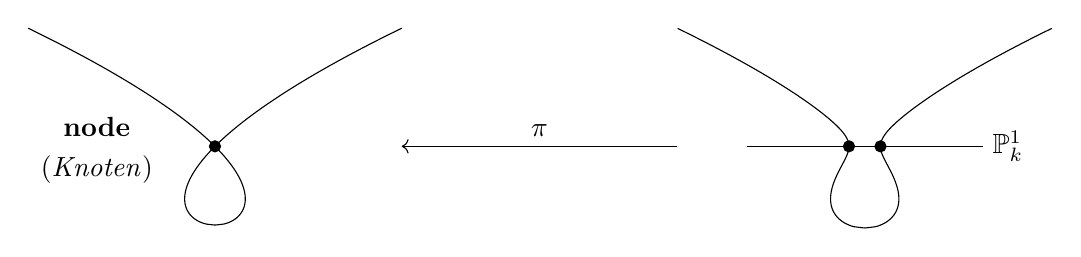
\begin{tikzpicture}
\newcommand{\ymax}{1.5}
\newcommand{\ymin}{-1.037184}
\newcommand{\linlen}{3}
\newcommand{\reg}{0.04}
\newcommand{\sep}{3.5}
\newcommand{\textsep}{1.5}
\newcommand{\ps}{2}

\newcommand{\cnode}{-sqrt((\ymax)^(2)+(\ymax)^(3))-\sep/2}
\newcommand{\cblup}{sqrt((\ymax)^(2)+(\ymax)^(3)+\reg)+\sep/2}
\draw [smooth,samples=75,domain=-1:0] plot({sqrt((\x)^(2)+(\x)^(3))+\cnode},\x);
\draw [smooth,domain=0:\ymax] plot({sqrt((\x)^(2)+(\x)^(3))+\cnode},\x);
\draw [smooth,samples=75,domain=-1:0] plot({-sqrt((\x)^(2)+(\x)^(3))+\cnode},\x);
\draw [smooth,domain=0:\ymax] plot({-sqrt((\x)^(2)+(\x)^(3))+\cnode},\x);
\draw [fill] ({\cnode},0) circle (\ps pt);
\draw [smooth,samples=150,domain=\ymin:\ymax] plot({sqrt((\x)^(2)+(\x)^(3)+\reg)+\cblup},\x);
\draw [smooth,samples=150,domain=\ymin:\ymax] plot({-sqrt((\x)^(2)+(\x)^(3)+\reg)+\cblup},\x);
\draw [fill] ({\cblup+sqrt(\reg)},0) circle (\ps pt);
\draw [fill] ({\cblup-sqrt(\reg)},0) circle (\ps pt);
\draw ({\cblup-\linlen/2},0) -- ({\cblup+\linlen/2},0);
\draw [right] ({\cblup+\linlen/2},0) node {$\mathbb{P}_k^1$};
\draw [->] (\sep/2,0) -- (-\sep/2,0);
\draw [above] (0,0) node {$\pi$};
\draw [above] ({\cnode-\textsep},0) node {\textbf{node}};
\draw [below] ({\cnode-\textsep},0) node {(\emph{Knoten})};
\end{tikzpicture}
\end{center}

\item $Z_2=\{y^2-x^3=0\}$.

\begin{center}
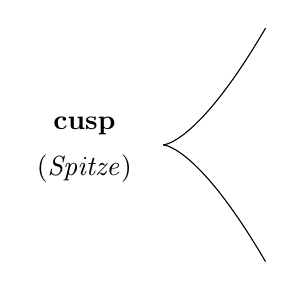
\begin{tikzpicture}
\newcommand{\xmax}{1.3}
\newcommand{\textsep}{1}

\draw [smooth,domain=0:\xmax] plot(\x,{sqrt(\x)^3});
\draw [smooth,domain=0:\xmax] plot(\x,{-sqrt(\x)^3});
\draw [above] (-\textsep,0) node {\textbf{cusp}};
\draw [below] (-\textsep,0) node {(\emph{Spitze})};
\end{tikzpicture}
\end{center}

\item $Z_3=\{y^2-x^5=0\}$.

\begin{center}
\begin{tikzpicture}
\newcommand{\xmax}{1.2}
\coordinate (text) at (-1,1);

\draw [smooth,domain=0:\xmax] plot(\x,{sqrt(\x)^5});
\draw [smooth,domain=0:\xmax] plot(\x,{-sqrt(\x)^5});
\draw (text) node {cusp};
\end{tikzpicture}
\end{center}
\end{enumerate}
\end{exercise}

\begin{comment}
From this, only the idea and the geometric intuition are expected, it doesn't need to be done rigorously. See Hartshorne \cite{hartshorne2013algebraic}.
\end{comment}

\begin{comment}
The key of this process is that, after being applied, although the singularity might not be solved, it becomes ``less singular'', so if we repeat the process, in the end we get a regular scheme.
\end{comment}

\begin{exercise}
$n=3$. $X_n=\{xy-z^n=0\}\subseteq\mathbb{A}_k^3$.

\begin{center}
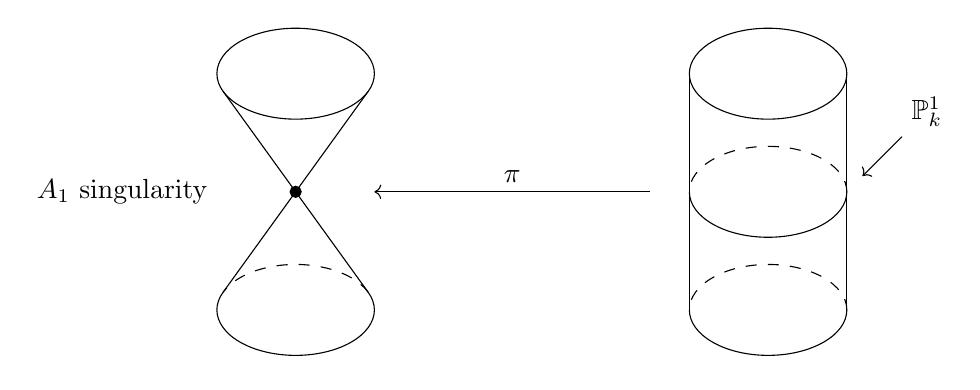
\begin{tikzpicture}
%ellipses: (x/a)^2+((y-h)/b)^2=1, (x/a)^2+((y+h)/b)^2=1
%tangency points: x=+-a*sqrt(1-(b/h)^2), y=+-((b/h)^2-h)
\newcommand{\hvar}{1.5}
\newcommand{\avar}{1}
\newcommand{\bvar}{sqrt(3)/3}
\newcommand{\sep}{3}
\newcommand{\pisep}{0.5}
\newcommand{\ps}{2}
\newcommand{\psep}{0.2}
\newcommand{\xlep}{0.5}

\newcommand{\xtan}{\avar*sqrt(1-(\bvar/\hvar)^2)}
\newcommand{\ytan}{-(\bvar)^2/\hvar+\hvar}
\draw (-\sep,\hvar) ellipse ({\avar} and {\bvar});
\draw [dash pattern=on 4pt off 4pt] ({\xtan-\sep},{-(\ytan)}) arc (acos((\xtan)/\avar):180-acos((\xtan)/\avar):{\avar} and {\bvar});
\draw ({-(\xtan)-\sep},{-(\ytan)}) arc (180-acos((\xtan)/\avar):360+acos((\xtan)/\avar):{\avar} and {\bvar});
\draw ({-(\xtan)-\sep},{\ytan}) -- ({\xtan-\sep},{-(\ytan)});
\draw ({\xtan-\sep},{\ytan}) -- ({-(\xtan)-\sep},{-(\ytan)});
\draw [fill] (-\sep,0) circle (\ps pt);
\draw (\sep,\hvar) ellipse ({\avar} and {\bvar});
\draw [dash pattern=on 4pt off 4pt] (\avar+\sep,-\hvar) arc (0:180:{\avar} and {\bvar});
\draw (-\avar+\sep,-\hvar) arc (180:360:{\avar} and {\bvar});
\draw [dash pattern=on 4pt off 4pt] (\avar+\sep,0) arc (0:180:{\avar} and {\bvar});
\draw (-\avar+\sep,0) arc (180:360:{\avar} and {\bvar});
\draw (-\avar+\sep,\hvar) -- (-\avar+\sep,-\hvar);
\draw (\avar+\sep,\hvar) -- (\avar+\sep,-\hvar);
\draw [->] (-\avar+\sep-\pisep,0) -- (\avar-\sep,0);
\draw [above] (-\pisep/2,0) node {$\pi$};
\draw [->] (\avar+\sep+\psep+\xlep,\psep+\xlep) -- (\avar+\sep+\psep,\psep);
\draw [above right] (\avar+\sep+\psep+\xlep,\psep+\xlep) node {$\mathbb{P}_k^1$};
\draw [left] (-\avar-\sep,0) node {$A_1$ singularity};
\end{tikzpicture}
\end{center}
\end{exercise}

Extra-reading (examples): Hartshorne \cite{hartshorne2013algebraic}, Chapter 1, \S 4.

\begin{definition}
$f:X\rightarrow Y$ morphism of schemes, $\mathcal{I}\subseteq\mathcal{O}_Y$ sheaf of ideals, $f^{-1}\mathcal{I}$ inverse image (as an abelian sheaf), have $f^{\sharp}:f^{-1}\mathcal{O}_Y\rightarrow\mathcal{O}_X$,
\[\alpha:f^{-1}\mathcal{I}\longrightarrow f^{-1}\mathcal{O}_Y\longrightarrow\mathcal{O}_X.\]
$f^{-1}\mathcal{I}\cdot\mathcal{O}_X$ or $\mathcal{I}\cdot\mathcal{O}_X$ is defined to be the ideal sheaf of $\mathcal{O}_X$ generated by the image of $\alpha$, the \textbf{inverse image ideal sheaf}.
\end{definition}

\begin{warning}
Do not confuse $f^{-1}\mathcal{I}\cdot\mathcal{O}_X$ with
\[f^*\mathcal{I}=f^{-1}\mathcal{I}\otimes_{f^{-1}\mathcal{O}_Y}\mathcal{O}_X.\]

There is a natural map
\[f^*\mathcal{I}\longrightarrow\mathcal{O}_X.\]
Its image is $f^{-1}\mathcal{I}\cdot\mathcal{O}_X$.
\end{warning}

\begin{proposition}
$X$ Noetherian scheme, $\mathcal{I}\subseteq\mathcal{O}_X$ coherent sheaf of ideals, $\pi:\widetilde{X}\rightarrow X$ blow-up of $\mathcal{I}$. Then:
\begin{enumerate}[label=\arabic*)]
\item $\pi^{-1}\mathcal{I}\cdot\mathcal{O}_{\widetilde{X}}=\widetilde{\mathcal{I}}$ is an invertible sheaf of $\widetilde{X}$;
\item if $Y$ is the closed subscheme of $X$ corresponding to $\mathcal{I}$ and $U\coloneqq X-Y$, then $\pi^{-1}(U)\rightarrow U$ is an isomorphism.
\end{enumerate}
\end{proposition}

\begin{proof}
\begin{enumerate}[label=\arabic*)]
\item $\widetilde{X}=\relProj\mathcal{S}\rightarrow X$, where $\mathcal{S}=\bigoplus_{d\geq0}\mathcal{I}^d$. If $U\subseteq X$ open affine,
\[\pi^{-1}(U)=\Proj\underbrace{\mathcal{S}(U)}_{\mathclap{\bigoplus\mathcal{I}(U)^d}}\longrightarrow\underbrace{\Spec R}_U.\]
\[\mathcal{O}(1)|_{\pi^{-1}(U)}=\widetilde{\bigoplus_{d\geq0}\mathcal{I}(U)^{d+1}}.\]
Check:
\[\mathcal{I}_U\cdot\mathcal{O}_{\pi^{-1}(U)}=\bigoplus_{d\geq0}\mathcal{I}_U^{d+1}=\mathcal{O}_{\pi^{-1}(U)}(1).\]
\[\mathcal{I}_U\cdot\mathcal{O}_{\pi^{-1}(U)}\cong\mathcal{O}_{\pi^{-1}(U)}(1),\]
the isomorphism is canonical.
\[\mathcal{I}\cdot\mathcal{O}_{\widetilde{X}}=\mathcal{O}_{\widetilde{X}}(1),\]
which is an invertible $\mathcal{O}_{\widetilde{X}}$-module.

\item If $U=X-Y$ is as above, then $\mathcal{I}|_U=\mathcal{O}_U$.
\[\pi^{-1}(U)=\relProj\bigoplus_{d\geq0}\mathcal{O}_U^{\oplus d}=\relProj\mathcal{O}_U[T]\overset{\cong}{\longrightarrow}U.\]
\end{enumerate}
\end{proof}

\begin{proposition}
\emph{\textbf{(Universal property of blow-up)}} Let $X$ Noetherian scheme, let $\mathcal{I}\subseteq\mathcal{O}_X$ coherent sheaf of ideals, let $\pi:\widetilde{X}\rightarrow X$ blow-up of $\mathcal{I}$. If $f:Z\rightarrow X$ is a morphism of schemes such that $f^{-1}\mathcal{I}\cdot\mathcal{O}_Z$ is an invertible sheaf of ideals on $Z$, then there exists a unique morphism $g:Z\rightarrow\widetilde{X}$ such that
\[
\begin{tikzcd}
Z\arrow[r,dashed,"\exists_{1\text{-}1}g"]\arrow[rd,"f",swap]&\widetilde{X}\arrow[d,"\pi"]\\
&X.
\end{tikzcd}
\]
\end{proposition}

\begin{proof}
W.l.o.g. $X$ is affine, say $X=\Spec R$ (by uniqueness this will glue to the general case). $R$ Noetherian ring, so $\mathcal{I}\subseteq\mathcal{O}_X$ transforms into $I\subseteq R$ a finitely generated ideal.
\[\widetilde{X}=\Proj\underset{\mathclap{\substack{\\||\\\bigoplus_{d\geq0}I^d}}}{S}\longrightarrow\Spec R=X.\]

Choose generators $I=(a_0,\ldots,a_n)$.
\begin{align*}
\varphi:R[y_0,\ldots,y_n]&\longrightarrow S=\bigoplus S_d\\
R\ni r&\longmapsto r\in S_0=R\\
y_i&\longmapsto a_i\in S_1=I
\end{align*}
is a surjective homomorphism of graded $R$-algebras.

This gives rise to
\[
\begin{tikzcd}
\widetilde{X}\arrow[rr,hook,"\text{closed immersion}"]\arrow[rd]&&\mathbb{P}_R^n\arrow[ld]\\
&X=\Spec R.
\end{tikzcd}
\]

$\ker\varphi$ is a homogeneous ideal generated by homogeneous polynomials $F\in R[x_0,\ldots,x_n]$ such that $F(a_0,\ldots,a_n)=0$.

Let $f:Z\rightarrow X$ be such that $\mathcal{L}\coloneqq f^{-1}\mathcal{I}\cdot\mathcal{O}_Z$ is an invertible $\mathcal{O}_Z$-module.

Have $I=(a_0,\ldots,a_n)$, $a_i\in\Gamma(X,\mathcal{I})=I$. Get global sections $f^{-1}a_i\eqqcolon s_i\in\Gamma(Z,\mathcal{L})$.

Check: they generate $\mathcal{L}$ globally.
\[
\begin{tikzcd}
Z\arrow[rr,"g"]\arrow[rd]&&\mathbb{P}_R^n\arrow[r,symbol={=}]\arrow[ld]&[-0.8cm]\Proj R[x_0,\ldots,x_n]\\
&\Spec R=X
\end{tikzcd}
\]

$g^*\mathcal{O}_{\mathbb{P}_R^n}(1)=\mathcal{L}$, $g^*x_i=s_i$.

\begin{claim}
%Claim/exc
$g$ factors through
\[
\begin{tikzcd}
\widetilde{X}\arrow[r,symbol=\subseteq]\arrow[rd,"\pi",swap]&[-1cm]\mathbb{P}_R^n\arrow[d]\\
&\Spec R.
\end{tikzcd}
\]
\end{claim}

Hint: ($\ker\varphi$ homogeneous of degree $d$) $F\in\ker\varphi\Leftrightarrow F(a_0,\ldots,a_n)=0\Rightarrow F(s_0,\ldots,s_n)=0$ in $\Gamma(Z,\mathcal{L}^{\otimes d})$.

\[
\begin{tikzcd}
g:Z\arrow[r]\arrow[rd]&\widetilde{X}\arrow[r,symbol=\subseteq]\arrow[d]&[-0.8cm]\mathbb{P}_R^n\\
&X
\end{tikzcd}
\]
\end{proof}

\begin{corollary}
$f:Y\rightarrow X$ morphism of Noetherian schemes, $\mathcal{I}\subseteq\mathcal{O}_X$ coherent sheaf of ideals, $\pi:\widetilde{X}=\Bl_{\mathcal{I}}(X)\rightarrow X$ blow-up of $\mathcal{I}$, $\widetilde{Y}\rightarrow Y$ blow-up of $f^{-1}\mathcal{I}\cdot\mathcal{O}_Y$. Then there exists a unique morphism $\tilde{f}:\widetilde{Y}\rightarrow\widetilde{X}$ such that
\[
\begin{tikzcd}
\widetilde{Y}\arrow[r,dashed,"\exists_{1\text{-}1}\tilde{f}"]\arrow[d]&\widetilde{X}\arrow[d]\\
Y\arrow[r,"f"]&X.
\end{tikzcd}
\]
Moreover, if $f$ is a closed immersion, then $\tilde{f}$ is a closed immersion.
\end{corollary}

\begin{proof}
Existence and uniqueness of $\tilde{f}$ follow from previous proposition.

\begin{exercise}
If $f$ is a closed immersion, then so is $\tilde{f}$.
\end{exercise}
\end{proof}

\begin{definition}
If $Y\subseteq X$ is a closed subscheme ($f$ is a closed immersion), then $\widetilde{Y}\subseteq\widetilde{X}$ is called the \textbf{strict transform} of the blow-up $\pi:\widetilde{X}\rightarrow X$.
\end{definition}

\section{Birational geometry}
%Section 16
\begin{definition}
$k$ algebraically closed field.
\begin{itemize}
\item A \textbf{variety over $\boldsymbol{k}$} is an integral, separated scheme of finite type over $k$,
\item a \textbf{complete variety} is a variety and proper over $k$,
\item a \textbf{projective variety} is a variety and projective over $k$,
\item a \textbf{quasi-projective variety} is an open subscheme of a projective variety.
\end{itemize}
\end{definition}

\begin{definition}
(Sloppy) A \textbf{rational map} between two varieties $f:X\dashrightarrow Y$ is a morphism $U\rightarrow Y$, where $U\subseteq X$ is open and dense.
\end{definition}

\begin{definition}
(More precise) A \textbf{rational map} of varieties $f:X\dashrightarrow Y$ is an equivalence class of pairs $\langle U,f_U\rangle$ where $U\subseteq X$ open dense, $f_U:U\rightarrow Y$. Equivalence relation:
\[\langle U,f_U\rangle\sim\langle V,f_V\rangle\Longleftrightarrow f_U|_{U\cap V}=f_V|_{U\cap V}.\]
A rational map is called \textbf{dominant} if $f_U(U)\subseteq Y$ is dense for some representative $\langle U,f_U\rangle$.
\end{definition}

\begin{definition}
A \textbf{birational map} $f:X\dashrightarrow Y$ is a rational map that admits an inverse $g:Y\dashrightarrow X$, $f\circ g\sim\id_Y$, $g\circ f\sim\id_X$.

$X,Y$ are said to be \textbf{birationally equivalent} if $\exists f:X\dashrightarrow Y$ birational.
\end{definition}

\begin{exercise}
This is equivalent to $\exists U\subseteq X$ open dense, $\exists V\subseteq Y$ open dense such that $U\cong V$.
\end{exercise}

\begin{definition}
A variety is called \textbf{rational} if it is birationally equivalent to $\mathbb{A}_k^n$ for some $n$ (equivalent to $\mathbb{P}_k^n$ for some $n$).
\end{definition}

%21/12
%online
\begin{theorem}
$k$ algebraically closed field, $X,Y$ varieties over $k$. There exists a bijection
\[\{f:X\dashrightarrow Y\text{ dominant rational maps}\}\longleftrightarrow\{k\text{-algebra homomorphisms }k(X)\leftarrow k(Y)\}.\]
\end{theorem}

\begin{proof}
``$\rightarrow$'' Given $f:X\dashrightarrow Y$, have
\begin{align*}
f_U:U&\longrightarrow Y,\\
\eta_X&\longmapsto\eta_Y
\end{align*}
\[f^{\sharp}:\underset{\substack{\\||\\\mathcal{O}_{U,\eta_X}\\\\||\\\\k(X)}}{\mathcal{O}_{X,\eta_X}}\longleftarrow\underset{\substack{\\||\\\\k(Y)}}{\mathcal{O}_{Y,\eta_Y}}.\]

``$\leftarrow$'' Given
\[
\begin{tikzcd}
k(Y)\arrow[r,"\varphi"]\arrow[d,symbol={=}]&k(X)\arrow[d,symbol={=}]\\[-0.4cm]
\mathcal{O}_{Y,\eta_Y}&\mathcal{O}_{X,\eta_X}
\end{tikzcd}
\]
$\exists U\subseteq X,V\subseteq Y$ open dense, $f:U\rightarrow V$ inducing $\varphi$.
\[f:X\dashrightarrow Y.\]
\end{proof}

\begin{corollary}
$X,Y$ varieties over algebraically closed $k$. TFAE:
\begin{enumerate}[label=\arabic*)]
\item $X$ and $Y$ are birationally equivalent;
\item $\exists U\subseteq X$, $\exists V\subseteq Y$ open dense with $U\cong V$;
\item $k(X)\cong k(Y)$ as $k$-algebras.
\end{enumerate}
\end{corollary}

\begin{proof}
Exercise (see notes).
\end{proof}

\begin{proposition}
$X$ algebraic variety over algebraically closed $k$, $\dim X=n$. Then $\exists Y\subseteq\mathbb{P}_k^{n+1}$ hypersurface that is birationally equivalent to $X$.
\end{proposition}

\begin{warning}
In general, one cannot choose $Y$ to be smooth over $k$.
\end{warning}

\begin{proof}
(Sketch) $k(X)$ is finitely generated over $k$. $k$ algebraically closed; in particular, $k$ perfect.
\[\exists k\underbrace{\lhook\joinrel\longrightarrow}_{\mathclap{\text{purely transcendental}}}k(x_1,\ldots,x_n)\underbrace{\lhook\joinrel\longrightarrow}_{\mathclap{\text{finite \& separable}}}k(X),\]

By theorem of primitive element, $k(X)=k(x_1,\ldots,x_n)(\alpha)$ for some $\alpha\in k(X)$. $\exists f_1\in k(x_1,\ldots,x_n)[y]$ irreducible polynomial, $f_1\neq0$, with $f_1(\alpha)=0$. Clear denominators, $\exists f\in k[x_1,\ldots,x_n,y]$ irreducible polynomial, $f(\alpha)=0$.

$Y_1\coloneqq\{f=0\}\subseteq\mathbb{A}_k^{n+1}$. $k(Y_1)=k(x_1,\ldots,x_n)(\alpha)=k(X)$. Hence, $X$ birationally equivalent to $Y_1$.
\[Y_1\lhook\joinrel\longrightarrow\mathbb{A}_k^{n+1}\lhook\joinrel\longrightarrow\mathbb{P}_k^{n+1}.\]
$Y\coloneqq\overline{Y_1}$ closure in $\mathbb{P}_k^{n+1}$, $k(Y_1)\cong k(Y)$, $Y_1$ and $Y$ birational.
\end{proof}

Back to blow-ups.

\begin{proposition}
$X$ algebraic variety over algebraically closed $k$, $\mathcal{I}\subseteq\mathcal{O}_X$ sheaf of ideals, $\mathcal{I}\neq0$, $\pi:\widetilde{X}\coloneqq\Bl_{\mathcal{I}}X\rightarrow X$ blow-up of $\mathcal{I}$. Then:
\begin{enumerate}[label=\arabic*)]
\item $\widetilde{X}$ is also a variety over $k$;
\item $\pi$ is a proper, birational, surjective morphism;
\item if $X$ is (quasi-)projective, then $\widetilde{X}$ is (quasi-)projective and $\pi$ is a projective morphism.
\end{enumerate}
\end{proposition}

\begin{proof}
\begin{enumerate}[label=\arabic*)]
\item $X$ is integral, $\mathcal{S}=\bigoplus_{d\geq0}\mathcal{I}^d$ is a sheaf of integral domains on $X$. Then $\widetilde{X}=\relProj\mathcal{S}$ is an integral scheme. $\pi$ is a proper morphism, so it is separated and of finite type.
\[
\begin{tikzcd}
\widetilde{X}\arrow[r,"\text{f.t.}","\text{sep.}"']\arrow[rr,bend right,"\text{f.t.}","\text{sep.}"']&X\arrow[r,"\text{f.t.}","\text{sep.}"']&\Spec k.
\end{tikzcd}
\]
Hence, $\widetilde{X}$ is a variety over algebraically closed $k$.

\item $\pi$ is proper, so it is a closed morphism. $\pi(\widetilde{X})\subseteq X$ is a closed subset. $Y$ be a closed subscheme corresponding to $\mathcal{I}$. Since $\mathcal{I}\neq0$, $Y\neq X$.

$U\coloneqq X-Y$ is open and dense. $\pi^{-1}(U)\rightarrow U$ is an isomorphism. Hence, $\pi$ is birational.

\[\emptyset\neq U\underset{\mathclap{\text{open}}}{\subseteq}\pi(\widetilde{X})\underset{\mathclap{\text{closed}}}{\subseteq}X.\]
Thus, $\pi(\widetilde{X})=X$, meaning that $\pi$ is surjective.

\item Exercise.
\end{enumerate}
\end{proof}

\begin{theorem}
Let $X$ quasi-projective variety over algebraically closed $k$, let $Z$ variety over $k$, let $f:Z\rightarrow X$ birational, projective morphism. Then $\exists\mathcal{I}\subseteq\mathcal{O}_X$ coherent sheaf of ideals such that
\[
\begin{tikzcd}
&[-0.8cm]Z\arrow[r]\arrow[d,-,double equal sign distance,double,"\cong"]&X\\[-0.1cm]
\widetilde{X}\arrow[r,symbol={=}]&\Bl_{\mathcal{I}}X.\arrow[ru]
\end{tikzcd}
\]
\end{theorem}

\begin{proof}
Hard. Hartshorne \cite{hartshorne2013algebraic} Chapter II, Theorem 7.17.
\end{proof}

\begin{example}
%Example/Application
$X\rightarrow\Spec R$ Noetherian scheme, $\mathcal{L}$ invertible $\mathcal{O}_X$-module, $s_0,\ldots,s_n\in\Gamma(X,\mathcal{L})$, $U$ the open set of $X$ where the $s_i$ generate $\mathcal{L}\subseteq X$.
\[\exists\varphi_U:U\longrightarrow\mathbb{P}_R^n.\]

\begin{construction}
$\mathcal{F}\subseteq\mathcal{L}$ be the coherent subsheaf generated by the $\{s_i\}$ if $V\subseteq X$ is open with $\mathcal{L}|_V\cong\mathcal{O}_V$. Let $\psi:\mathcal{L}|_V\xrightarrow{\cong}\mathcal{O}_V$, $\mathcal{I}|_V\coloneqq\psi(\mathcal{F}|_V)\subseteq\mathcal{O}_V$. Get an ideal sheaf on $X$ $\mathcal{I}\subseteq\mathcal{O}_X$ such that $\mathcal{I}_x=\mathcal{O}_{X,x}\Leftrightarrow x\in U$.

Let $Y\subseteq X$ be the closed subscheme defined by $\mathcal{I}$, $\supp Y=X-U$. Consider the blow-up $\widetilde{X}=\Bl_{\mathcal{I}}X\rightarrow X$ note $\pi^{-1}\mathcal{I}\cdot\mathcal{O}_{\widetilde{X}}$ is invertible $\mathcal{O}_{\widetilde{X}}$-module. $\pi^*s_i$ give global sections of $\pi^*\mathcal{L}$.

\[
\begin{tikzcd}
\widetilde{X}\arrow[r,symbol=\supseteq]\arrow[d,"\pi",swap]\arrow[rrd,bend left=60,"\varphi"]&[-0.6cm]\pi^{-1}(U)\arrow[d,"\cong",swap]\\
X&U\arrow[l,hook']\arrow[r,"\varphi_U",swap]&\mathbb{P}_R^n
\end{tikzcd}
\]

Get a morphism $\varphi:\widetilde{X}\rightarrow\mathbb{P}_R^n$. $\varphi|_{\pi^{-1}(U)}=\varphi_U$ \textbf{resolution of indeterminacy}.
\end{construction}
\end{example}

\begin{example}
(Cremona transformation)
\begin{align*}
\varphi:\mathbb{P}_k^2&\dashrightarrow\mathbb{P}_k^2,\\
[x:y:z]&\longmapsto\left[\frac{1}{x}:\frac{1}{y}:\frac{1}{z}\right]=\left[\frac{xyz}{x}:\frac{xyz}{y}:\frac{xyz}{z}\right]=[yz:xz:xy]
\end{align*}
\textbf{quadratic transformation}. Birational self-map not defined at $[1:0:0],[0:1:0],[0:0:1]$. Blow-up:
\[
\begin{tikzcd}
&S\arrow[ld,"\pi",swap]\arrow[rd,"\tilde{\varphi}"]\\
\mathbb{P}_k^2\arrow[rr,dashed,"\varphi"]&&\mathbb{P}_k^2.
\end{tikzcd}
\]

Hartshorne \cite{hartshorne2013algebraic} Chapter V, Example 4.2.3.

$\varphi\in\Bir(\mathbb{P}_k^2)=\Cr_2(k)\supseteq\Aut(\mathbb{P}_k^2)$ the Cremona group.
\end{example}

\begin{theorem}
\emph{\textbf{(Castelnuovo, M. Noether, $\boldsymbol{+\epsilon}$)}} $\varphi$ and $\Aut(\mathbb{P}_k^2)$ generate $\Cr_2(k)$.
\end{theorem}

\subsection*{Resolution of singularities}
$X$ a (quasi-projective) variety over algebraically closed $k$.

\begin{recall}
$X=\bigcup U_{\alpha}$, $U_{\alpha}=\Spec R_{\alpha}$, $R_{\alpha}\subseteq\widetilde{R}_{\alpha}\subseteq\Quot(R_{\alpha})$, $\widetilde{R}_{\alpha}$ the integral closure.

$\Spec R_{\alpha}\leftarrow\Spec\widetilde{R}_{\alpha}$ glues $\nu:X^{\nu}\rightarrow X$, \textbf{normalisation}.

$X^{\nu}$ is a normal variety over algebraically closed $k$.
\end{recall}

\begin{fact}
$X_{\text{sm}}$ open dense subscheme where $X$ is smooth.

If $X$ is normal, then $X_{\text{sing}}\coloneqq X-X_{\text{sm}}$ has $\codim\geq2$.

If $X$ is a curve, $\nu:X^{\nu}\rightarrow X$ will be smooth.
\end{fact}

\begin{question}\label{question_resolution}
Let $X$ be a variety over algebraically closed $k$. Does there exist $\pi:Y\rightarrow X$ proper and birational with $Y$ smooth over $k$ (``\textbf{resolution of singularities}'')?
\end{question}

\begin{question}\label{question_isomorphism}
In Question \ref{question_resolution}, does there exist $\pi$ such that $\pi^{-1}(X_{\text{sm}})\rightarrow X_{\text{sm}}$ is an isomorphism?
\end{question}

\begin{question}\label{question_log-resolution}
In Question \ref{question_isomorphism}, does there even exist $\pi$ such that
\begin{enumerate}[label=\roman*)]
\item $\pi^{-1}(X_{\text{sm}})\rightarrow X_{\text{sm}}$ an isomorphism;
\item $\pi^{-1}(X\setminus X_{\text{sm}})$ is a divisor with normal crossings?

\begin{center}
\begin{tikzpicture}
\newcommand{\xpar}{2}
\newcommand{\para}{0.1}
\newcommand{\yhyp}{1}
\newcommand{\xnode}{0.5}
\newcommand{\xstar}{0.75}
\newcommand{\ybar}{1.5}
\newcommand{\sep}{1.5}

\draw [smooth,domain=-\yhyp:\yhyp] plot({sqrt((\x)^2+1)-\sep-\xpar},\x);
\draw [smooth,domain=-\yhyp:\yhyp] plot({-sqrt((\x)^2+1)-\sep-\xpar},\x);
\draw [smooth,domain=-\xpar:\xpar] plot(\x-\sep-\xpar,{\para*(\x)^2});
\draw (0,-\ybar) -- (0,\ybar);
\draw [samples=75,smooth,domain=-1:0] plot(\x+\sep+1,{sqrt((\x)^2+(\x)^3)});
\draw [smooth,domain=0:\xnode] plot(\x+\sep+1,{sqrt((\x)^2+(\x)^3)});
\draw [samples=75,smooth,domain=-1:0] plot(\x+\sep+1,{-sqrt((\x)^2+(\x)^3)});
\draw [smooth,domain=0:\xnode] plot(\x+\sep+1,{-sqrt((\x)^2+(\x)^3)});
\draw (2*\sep+1+\xnode,0) -- (2*\xstar+2*\sep+1+\xnode,0);
\draw (\xstar+2*\sep+1+\xnode,\xstar) -- (\xstar+2*\sep+1+\xnode,-\xstar);
\draw (2*\sep+1+\xnode,\xstar) -- (2*\xstar+2*\sep+1+\xnode,-\xstar);
\draw (2*\sep+1+\xnode,-\xstar) -- (2*\xstar+2*\sep+1+\xnode,\xstar);
\draw (3*\sep/2+1+\xnode,\ybar) node {not};
\end{tikzpicture}
\end{center}

(``\textbf{log-resolution}'')
\end{enumerate}
\end{question}

\textbf{State of the art} (what is known?)

\textbf{dim 1}: yes for Q\ref{question_resolution}-Q\ref{question_log-resolution}.

\textbf{dim 2}: yes for Q\ref{question_resolution}-Q\ref{question_log-resolution}.
\begin{itemize}[label=$-$]
\item Italian school 19\textsuperscript{th} century.
\item Walker (1930) $\chara k=0$.
\item Abhyankar (1956) $\chara k\neq0$.
\end{itemize}

$\boldsymbol{\chara k=0}$: yes for Q\ref{question_resolution}-Q\ref{question_log-resolution}. Hironaka (1964).

\textbf{dim 3}: $\chara k\geq7$ yes for Q\ref{question_resolution}-Q\ref{question_log-resolution}. Abhyankar (1966).

\begin{definition}
$X$ algebraic variety over $k$. An \textbf{alteration} of $X$ is a $\pi:Y\rightarrow X$ such that $Y$ is smooth over $k$, $\pi$ is surjective and generically finite, i.e., $\exists U\subseteq X$ open dense such that $\pi^{-1}(U)\rightarrow U$ is a finite morphism.
\end{definition}

\begin{theorem}
\emph{\textbf{(de Jong, 1996)}} Alterations exist.
\end{theorem}

%09/01/2023
%online
\stepcounter{section}
\section{Cohomology}
%Section 18
Given $(X,\mathcal{O}_X)$ scheme, a short exact sequence of $\mathcal{O}_X$-modules
\[0\longrightarrow\mathcal{F}'\longrightarrow\mathcal{F}\longrightarrow\mathcal{F}''\longrightarrow0,\]
consider global sections
\[
\begin{tikzcd}
0\arrow[r]&\underset{\substack{||\\\Gamma(X,\mathcal{F}')\\||\\H^0(X,\mathcal{F}')}}{\mathcal{F}'(X)}\arrow[r]&\mathcal{F}(X)\arrow[r]&\mathcal{F}''(X)\arrow[out=0,in=180,looseness=2,overlay,lld]\\
&H^1(X,\mathcal{F}')\arrow[r]&H^1(X,\mathcal{F})\arrow[r]&H^1(X,\mathcal{F}'')\arrow[out=0,in=180, looseness=2,overlay,lld]\\
&H^2(X,\mathcal{F}')\arrow[r]&\cdots
\end{tikzcd}
\]
Want: long exact sequence.

Objectives:
\begin{itemize}[label=$-$]
\item $H^i(X,\mathcal{F})$ should exist ``natural, functorial, minimal'';
\item ideally:
\begin{itemize}[label=$-$]
\item finiteness results,
\item vanishing results,
\item computable.
\end{itemize}
\end{itemize}

Let $(X,\mathcal{O}_X)$ be a scheme.

\begin{definition}
An \textbf{injective sheaf} (of abelian groups or $\mathcal{O}_X$-modules) is a sheaf $\mathcal{I}$ on $X$ such that for all sheaves $\mathcal{F},\mathcal{G}$ and all morphisms
\[
\begin{tikzcd}
\mathcal{F}\arrow[rr,"f\text{ injective}"]\arrow[d,"g",swap]&&\mathcal{G}\arrow[lld,dashed,"\exists h"]\\
\mathcal{I}
\end{tikzcd}
\]
this commutes; in other words, the functor $\Hom(-,\mathcal{I})$ is exact (small exercise).
\end{definition}

\begin{example}
$\mathbb{Q}/\mathbb{Z}$ is an injective $\mathbb{Z}$-module.
\end{example}

\begin{definition}
An \textbf{injective resolution} of a sheaf $\mathcal{F}$ on $X$ is an exact sequence
\[0\longrightarrow\mathcal{F}\overset{\epsilon}{\longrightarrow}I^0\longrightarrow I^1\longrightarrow\cdots\]
where the $I^i$ are injective sheaves on $X$.
\end{definition}

\begin{theorem}
The categories of abelian sheaves and of $\mathcal{O}_X$-modules on a scheme $X$ have \textbf{enough injectives}, that is, for every sheaf $\mathcal{F}$ on $X$, there exists an injective sheaf $I$ and an injection $\mathcal{F}\rightarrow I$.
\end{theorem}

\begin{corollary}
Let $\mathcal{F}$ be a sheaf on $X$. Then, there exists an injective resolution of $\mathcal{F}$.
\end{corollary}

\begin{proof}
By theorem, there exists
\[0\longrightarrow\mathcal{F}\overset{\epsilon}{\longrightarrow}I^0\]
for some $I^0$ injective. Get
\[0\longrightarrow\mathcal{F}\longrightarrow I^0\longrightarrow I^0/\mathcal{F}\longrightarrow0.\]
$\exists I^1$ injective sheaf and
\[0\longrightarrow I^0/\mathcal{F}\longrightarrow I^1\longrightarrow I^1/(I^0/\mathcal{F})\longrightarrow0.\]
$\exists I^2$ injecitve sheaf and
\[0\longrightarrow I^1/(I^0/\mathcal{F})\longrightarrow I^2\]
\[\cdots\]
Continue this to
\[
\begin{tikzcd}
0\arrow[r]&\mathcal{F}\arrow[r,"\epsilon"]&I^0\arrow[r]\arrow[rd]&I^0/\mathcal{F}\arrow[r]\arrow[d,hook']&0\\
&&&I^1
\end{tikzcd}
\]
\[
\begin{tikzcd}
0\arrow[r]&\mathcal{F}\arrow[r]&I^0\arrow[r]&I^1,
\end{tikzcd}
\]
etc.
\end{proof}

\begin{recall}
A sheaf $\mathcal{F}$ on $X$ is called \textbf{flasque} if $\forall V\subseteq U\subseteq X$ (inclusions of open sets) the restriction map
\[\mathcal{F}(U)\longrightarrow\mathcal{F}(V)\]
is surjective.
\end{recall}

\begin{lemma}
Injective sheaves are flasque.
\end{lemma}

\begin{proof}
(Sketch) Let $U\subseteq X$ be open. Consider $j:U\rightarrow X$ inclusion map and $j_!(\mathcal{O}_X|_U)$. Now, let $\mathcal{I}$ be an injective $\mathcal{O}_X$-module. Let $V\subseteq U\subseteq X$ be an inclusion of open sets. Get an exact sequence (check!)
\[0\longrightarrow j_!(\mathcal{O}_X|_V)\longrightarrow j_!(\mathcal{O}_X|_U).\]
Since $\mathcal{I}$ is injective,
\[\Hom\big(j_!(\mathcal{O}_X|_U),\mathcal{I}\big)\longrightarrow\Hom\big(j_!(\mathcal{O}_X|_V),\mathcal{I}\big)\]
is surjective, which corresponds to
\[\mathcal{I}(U)\xrightarrow[\text{restriction}]{}\mathcal{I}(V),\]
which is onto.
\end{proof}

\begin{recall}
\[0\longrightarrow\mathcal{F}'\longrightarrow\mathcal{F}\longrightarrow\mathcal{F}''\longrightarrow0\]
an exact sequence of $\mathcal{O}_X$-modules, then
\[0\longrightarrow\mathcal{F}'(X)\longrightarrow\mathcal{F}(X)\longrightarrow\mathcal{F}''(X)\]
is exact and if $\mathcal{F}'$ is flasque, then
\[\mathcal{F}(X)\longrightarrow\mathcal{F}''(X)\longrightarrow0\]
is exact.
\end{recall}

\begin{definition}
For a sheaf $\mathcal{F}$ on $X$, choose an injective resolution
\[0\longrightarrow\mathcal{F}\overset{\epsilon}{\longrightarrow}I^0\longrightarrow I^1\longrightarrow\cdots\]
Take global sections
\[0\longrightarrow\mathcal{F}(X)\overset{\epsilon}{\longrightarrow}I^0(X)\overset{d_0}{\longrightarrow}I^1(X)\overset{d_1}{\longrightarrow}\cdots\]
This is a complex and take cohomology of this complex
\[H^*(X,\mathcal{F}),\]
where
\[H^i(X,\mathcal{F})=\frac{\ker d_i}{\im d_{i-1}}.\]
\end{definition}

\begin{exercise}
$H^0(X,\mathcal{F})=\mathcal{F}(X)$.
\end{exercise}

\begin{fact}
\begin{itemize}[label=$-$]
\item This is well-defined and does not depend on the choice of injective resolution.
\item If
\[0\longrightarrow\mathcal{F}'\longrightarrow\mathcal{F}\longrightarrow\mathcal{F}''\longrightarrow0\]
is a short exact sequence of $\mathcal{O}_X$-modules, then you get a long exact sequence
\[
\begin{tikzcd}
0\arrow[r]&\overbrace{H^0(X,\mathcal{F}')}^{\mathcal{F}'(X)}\arrow[r]&\overbrace{H^0(X,\mathcal{F})}^{\mathcal{F}(X)}\arrow[r]&\overbrace{H^0(X,\mathcal{F}'')}^{\mathcal{F}''(X)}\arrow[out=0,in=180,looseness=2,overlay,lld,"\delta",swap]\\
&H^1(X,\mathcal{F}')\arrow[r]&H^1(X,\mathcal{F})\arrow[r]&\cdots
\end{tikzcd}
\]
\item If $\mathcal{I}$ is a flasque, then $H^i(X,\mathcal{I})=0$ $\forall i\geq1$.
\end{itemize}
\end{fact}

\begin{upshot}
$H^i(X,\mathcal{F})$ exist, natural, functorial, well-defined, long exact sequence.
\end{upshot}

\subsection*{Cohomology of affine schemes}
\begin{theorem}
Let $R$ be a Noetherian ring, let $X=\Spec R$, let $\mathcal{F}$ be a quasi-coherent $\mathcal{O}_X$-module. Then,
\[H^i(X,\mathcal{F})=0\ \ \forall i\geq1.\]
\end{theorem}

$H^i(X,\underline{\mathbb{Z}})$ (de Rham, Poincar\'{e}, Grothendieck), but $\underline{\mathbb{Z}}$ (constant sheaf) is not quasi-coherent $\mathcal{O}_X$-module (Serre).

\begin{proof}
(Sketch) By definition, we have $\mathcal{F}=\widetilde{M}$ for some $R$-module $M$. Choose an injective resolution of $M$ as an $R$-module
\[0\longrightarrow M\longrightarrow I^0\longrightarrow I^1\longrightarrow\cdots\]
Note: $\widetilde{}$\; is an exact functor.
\[0\longrightarrow\widetilde{M}\longrightarrow\widetilde{I}^0\longrightarrow\widetilde{I}^1\longrightarrow\cdots\]
is an exact sequence of $\mathcal{O}_X$-modules, where $\widetilde{M}=\mathcal{F}$ and (check!) $\widetilde{I}^i$ is injective.
\[0\longrightarrow\mathcal{F}\longrightarrow\widetilde{I}^0\longrightarrow\widetilde{I}^1\longrightarrow\cdots\]
is an injective resolution. Take global sections:
\[
\begin{tikzcd}
0\arrow[r]&\mathcal{F}(X)\arrow[r]\arrow[d,symbol={=}]&\widetilde{I}^0(X)\arrow[r]\arrow[d,symbol={=}]&\widetilde{I}^1(X)\arrow[r]\arrow[d,symbol={=}]&\cdots\\[-0.2cm]
0\arrow[r]&M\arrow[r]&I^0\arrow[r]&I^1,
\end{tikzcd}
\]
but this is the injective resolution of $M$ we started with. In particular, this complex is exact, so it has no higher non-zero cohomology. But this is the cohomology of $\mathcal{F}$. Hence,
\[H^i(X,\mathcal{F})=0\ \ \forall i\geq1.\]
\end{proof}

\begin{theorem}
\emph{\textbf{(Serre)}} Let $X$ be a Noetherian scheme. TFAE:
\begin{enumerate}[label=\arabic*)]
\item $X$ is affine;
\item for all quasi-coherent $\mathcal{O}_X$-modules $\mathcal{F}$, we have $H^i(X,\mathcal{F})=0$ $\forall i\geq1$;
\item for all quasi-coherent sheaves of ideals $\mathcal{I}\subseteq\mathcal{O}_X$, $H^1(X,\mathcal{I})=0$.
\end{enumerate}
\end{theorem}

\subsection*{\v{C}ech cohomology}
$X$ a scheme (or topological space), $\{U_i\}$ open cover (usually and in the sequel open and affine), $\mathcal{F}$ a sheaf of abelian groups (or $\mathcal{O}_X$-modules) on $X$. Also assume $U_i$ $i\in I$, $I\subseteq\mathbb{N}$ and finite. Define \textbf{\v{C}ech complex}
\[C^p\coloneqq\prod_{\substack{i_0<\cdots<i_p\\i_i\in I}}\mathcal{F}(U_{i_0}\cap\cdots\cap U_{i_p}).\]
\[C^p=0\left\{\begin{array}{ll}\text{if}&p<0,\\\text{if}&p\geq|I|.\end{array}\right.\]
\textbf{Differential} $C^p\rightarrow C^{p+1}$.

If $\alpha\in C^p$, we have $\alpha_{i_0,\ldots,i_p}\in\mathcal{F}(U_{i_0}\cap\cdots\cap U_{i_p})$ for $i_0<\cdots<i_p$. Define $d\alpha\in C^{p+1}$ via
\[(d\alpha)_{i_0,\ldots,i_{p+1}}\coloneqq\sum_{k=0}^{p+1}(-1)^k\alpha_{i_0,\ldots,\widehat{i_k},\ldots,i_{p+1}},\ \ i_0<\cdots<i_{p+1}.\]
Check:
\[C^p\overset{d}{\longrightarrow}C^{p+1}\overset{d}{\longrightarrow}C^{p+2},\]
$d\circ d=0$, i.e., $(C^p,d)$ is a complex of abelian groups.

\begin{definition}
$\check H^p(\{U_i\},\mathcal{F})\coloneqq h^p(C^*)$ the cohomology of the complex $(C^p,d)$. \textbf{\v{C}eck cohomology} of $\mathcal{F}$ w.r.t. the cover $\{U_i\}$.
\end{definition}

\begin{example}
$k$ a field, $X=\mathbb{P}_k^1$ projective line, $\Omega_{X/k}=\mathcal{O}_X(-2)$ sheaf of K\"{a}hler differentials.
\[
\begin{tikzcd}
U=\Spec k[x]\arrow[r,symbol=\subseteq]&[-0.6cm]X\\
V=\Spec k[y]\arrow[ru,hook,"y=\frac{1}{x}",swap]
\end{tikzcd}
\]
standard affine cover.
\[C^0=\Omega(U)\times\Omega(V),\]
\[C^1=\Omega(U\cap V).\]
\[\Omega(U)=k[x]\cdot dx,\]
\[\Omega(V)=k[y]\cdot dy,\]
\[\Omega(U\cap V)=k\left[x,\frac{1}{x}\right]\cdot dx.\]
Differentials:
\begin{align*}
d:C^0&\longrightarrow C^1.\\
x&\longmapsto x\\
y&\longmapsto\frac{1}{x}\\
dy&\longmapsto d\left(\frac{1}{x}\right)=-\frac{1}{x^2}\,dx
\end{align*}
\[\ker\big(d:\underbrace{C^0\longrightarrow C^1}_{\mathclap{\substack{\Omega(U)\times\Omega(V)\longrightarrow\Omega(U\cap V)\\(k[x]\,dx)\oplus(k[y]\,dy)\longrightarrow k[x,\frac{1}{x}]\,dx}}}\big)=\left\{\big(f(x)\,dx,g(y)\,dy\big)\,\left|\,f(x)=-\frac{1}{x^2}g\left(\frac{1}{x}\right)\right.\right\}\]

\begin{exercise}
This can happen only if $f=g=0$.
\end{exercise}

Hence, $\ker d=0$.
\[\check H^0\big(\{U,V\},\Omega\big)=0.\]
Next,
\[\im d=\left\{\left(f(x)+\frac{1}{x^2}g\left(\frac{1}{x}\right)\right)dx\right\}\subseteq k\left[x,\frac{1}{x}\right]\,dx.\]
$\im d$ is the $k$-subvector space of $k[x,\frac{1}{x}]$ generated by $x^n\,dx$ with $n\in\mathbb{Z}$ but $n\neq-1$. Thus,
\[\check H^1\big(\{U,V\},\Omega\big)=\frac{k\left[x,\frac{1}{x}\right]dx}{\im d}\]
is $1$-dimensional and generated by $\frac{1}{x}\,dx$.
\end{example}

%11/12
\begin{lemma}
%Lemma/Exercise
$X$ topological space, $\{U_i\}$ open cover of $X$, $\mathcal{F}$ sheaf of abelian groups. Then,
\[\check H^0(\{U_i\},\mathcal{F})=\mathcal{F}(X).\]
\end{lemma}

\begin{proof}
(Sketch)
\[\check H^0=\ker(d:C^0\rightarrow C^1).\]
$\alpha\in C^0$, then $(\alpha_i)_{i\in I}$, $\alpha_i\in\mathcal{F}(U_i)$.
\[d\alpha=0\Longleftrightarrow\forall i\neq j\ \alpha_i-\alpha_j=0\text{ on }U_i\cap U_j\Longleftrightarrow\alpha_i|_{U_i\cap U_j}=\alpha_j|_{U_i\cap U_j}.\]
By sheaf axiom, these glue to some $\alpha\in\mathcal{F}(X)$ with $\alpha|_{U_i}=\alpha_i$.
\end{proof}

\begin{theorem}
Let $(X,\mathcal{O}_X)$ be a separated and Noetherian scheme. Let $\{U_i\}_{i\in I\subsetneqq\mathbb{N}}$ open affine cover of $X$. Let $\mathcal{F}$ be a quasi-coherent $\mathcal{O}_X$-module. Then there exists a natural isomorphism $\forall i\geq0$
\[\check H^i(\{U_i\},\mathcal{F})\longrightarrow H^i(X,\mathcal{F}).\]
\end{theorem}

(``\v{C}ech cohomology computes coherent cohomology.'')

Very generally,
\begin{itemize}
\item you can define $\mathcal{H}^j(\mathcal{F})$ cohomology sheaves
\[U\longmapsto H^j(U,\mathcal{F}|_U)\]
and sheafify.

$\check H^p(\{U_i\},\mathcal{H}^q(\mathcal{F}))$ leads by spectral sequence (Jean Leray 1910) to $H^{p+q}(X,\mathcal{F})$.

\item $\mathcal{H}^q(\mathcal{F})=0$ if $q\geq1$.

\item $H^p(U_{i_0}\cap\cdots\cap U_{i_p},\mathcal{F}|_{\cdots})=0$ $\forall p\geq1$, since the intersection of affines is affine in separated $X$.
\end{itemize}

\begin{example}
$k$ a field.
\[H^i\big(\mathbb{P}_k^1,\Omega_{\mathbb{P}_k^1}^1\big)=\left\{\begin{array}{ll}0&i\neq1,\\k&i=1.\end{array}\right.\]
\end{example}

\begin{remark}
$\mathcal{F}$ quasi-coherent $\mathcal{O}_X$-module on $X=\mathbb{P}_k^n$. There exists an open affine cover by $(n+1)$ sets. So,
\[H^i(\mathbb{P}_k^n,\mathcal{F})=0\ \ \forall i\geq n+1.\]
\end{remark}

\begin{theorem}
\emph{\textbf{(Grothendieck)}} Let $(X,\mathcal{O}_X)$ be a Noetherian scheme of dimension $d$, let $\mathcal{F}$ be a sheaf of abelian groups on $X$. Then
\[H^i(X,\mathcal{F})=0\ \ \forall i>d.\]
\end{theorem}

\begin{exercise}

Let $\mathbb{S}^1$ be the circle (in its usual topology), let $\mathbb{Z}$ be the constant sheaf $\mathbb{Z}$ and $U_1, U_2$ two connected open semi-circles that cover the circle and which overlap at each end, so that $U\cap V$ consists of two small intervals.

Calculate the cohomology groups and check that they are the following:
\[\check H^i(\{U_i\},\mathbb{Z})=\left\{\begin{array}{lll}\mathbb{Z}&\text{if}&i=1,2;\\0;\end{array}\right.\]
whith the differential map being
\begin{align*}
d:\mathbb{Z}\oplus\mathbb{Z}&\longrightarrow\mathbb{Z}^2\\
(x,y)&\longmapsto(x-y,y-x)
\end{align*}
\end{exercise}

Mayer-Vietoris is a special case of \v{C}ech cohomology.
%Example 4.0.4 from Hartshorne

\subsection*{Cohomology of $\boldsymbol{\mathbb{P}_k^n}$}
Use \v{C}ech cohomology to compute $H^i(\mathbb{P}_k^d,\mathcal{O}(n))$.

Idea: use standard cover $X=\mathbb{P}_R^d=\Proj R[x_0,\ldots,x_d]$, $U_i=D_+(x_i)$ standard open affine cover, $R$ Noetherian ring.

\begin{theorem}
Let $R$ be a Noetherian ring. Let $S=R[x_0,\ldots,x_d]$, $X=\mathbb{P}_R^d=\Proj S$.

\begin{enumerate}[label=\arabic*)]
\item The natural map
\[S\longrightarrow\Gamma_*(\mathcal{O}_X)\coloneqq\bigoplus_{n\in\mathbb{Z}}H^0\big(X,\mathcal{O}_X(n)\big)\]
is an isomorphism of $R$-algebras.

$\mathcal{L}$ on $X$, $\Gamma_*(\mathcal{F})=\bigoplus H^0(X,\mathcal{F}\otimes\mathcal{L}^{\otimes n})$.

\item $H^i(X,\mathcal{O}(n))=0$ $\forall n\in\mathbb{Z}$, $\forall i\notin\{0,d\}$.

\item $H^d(X,\underbrace{\mathcal{O}_X(-d-1)}_{\omega_X})\cong R$.

\item \emph{\textbf{(Serre duality)}} There is a natural pairing
\[H^0\big(X,\mathcal{O}_X(n)\big)\times H^d(X,\mathcal{O}_X(-n-d-1)\big)\longrightarrow H^d\big(X,\mathcal{O}_X(-d-1)\big)\cong R,\]
which is a perfect pairing of finitely generated free $R$-modules $\forall n\in Z$.

If $R$ is a field $k$,
\[H^d\big(X,\mathcal{O}_X(-n-d-1)\big)\cong\big(H^0\big(X,\mathcal{O}_X(n)\big)\big)^{\vee}.\]
\end{enumerate}
\end{theorem}

\begin{comment}
A pairing is just a bilinear map and ``perfect'' means that it is non-degenerate. Poincar\'{e} duality is a special case of Serre duality.
\end{comment}

\begin{theorem}
\emph{\textbf{(Serre)}} Let $R$ be a Noetherian ring, let $X\rightarrow\Spec R$ be a projective scheme, let $\mathcal{L}$ be a very ample invertible $\mathcal{O}_X$-module, let $\mathcal{F}$ be a coherent $\mathcal{O}_X$-module.

\begin{enumerate}[label=\arabic*)]
\item $\forall i\geq0$ $H^i(X,\mathcal{F})$ is a finitely generated $R$-module.

\item $\exists n_0=n_0(\mathcal{F})$ integer such that $\forall i\geq1$ $\forall n\geq n_0$
\[H^i(X,\mathcal{F}\otimes\mathcal{L}^{\otimes n})=0.\]
\end{enumerate}
\end{theorem}

\begin{comment}
This theorem is proven with the \emph{d\'{e}vissage} technique. It is reduced to the case that $X$ is the projective space, $\mathcal{L}$ is $\mathcal{O}(n)$ with $n>0$, and $\mathcal{F}$ is a quotient of direct sums of $\mathcal{L}$.
\end{comment}

\begin{proposition}
$R$ Noetherian ring, $X\rightarrow\Spec R$ proper scheme over $R$, $\mathcal{L}$ invertible $\mathcal{O}_X$-module. TFAE:
\begin{enumerate}[label=\arabic*)]
\item $\mathcal{L}$ is ample;
\item $\forall \mathcal{F}$ coherent $\mathcal{O}_X$-module $\exists n_0=n_0(\mathcal{F})$ such that
\[H^i(X,\mathcal{L}^{\otimes n}\otimes\mathcal{F})=0,\ \ i\geq1,n\geq n_0;\]
\end{enumerate}
\end{proposition}

\begin{definition}
$X\rightarrow\Spec k$ projective scheme over a field $k$, $\mathcal{F}$ coherent $\mathcal{O}_X$-module.
\[\chi(\mathcal{F})\coloneqq\sum_{i\in\mathbb{Z}}(-1)^i\dim_kH^i(X,\mathcal{F})\]
is called the \textbf{Euler (-Poincar\'{e}) characteristic} of $\mathcal{F}$.
\end{definition}

\begin{exercise}
If
\[0\longrightarrow\mathcal{F}'\longrightarrow\mathcal{F}\longrightarrow\mathcal{F}''\longrightarrow0\]
is an exact sequence of coherent $\mathcal{O}_X$-modules, then
\[\chi(\mathcal{F})=\chi(\mathcal{F}')+\chi(\mathcal{F}'').\]
\end{exercise}

\begin{definition}
$X\rightarrow\Spec k$ projective scheme over a field $k$.
\[p_a(X)\coloneqq(-1)^{\dim X}\big(\chi(\mathcal{O}_X)-1\big)\]
is called the \textbf{arithmetic genus} of $X$.
\end{definition}

\begin{exercise}
If $X$ is a curve (integral, projective, 1-dimensional) and $k$ algebraically closed, then
\[p_a(X)=\dim_kH^1(X,\mathcal{O}_X).\]
\end{exercise}

\begin{definition}
The \textbf{geometric genus} of $X$ is defined to be
\[p_g(X)=\dim_kH^0\big(X,\Omega_{X/k}^{\dim X}\big)\]
and
\[P_n(X)\coloneqq\dim_kH^0(X,(\Omega_{X/k}^{\dim X})^{\otimes n}\big)\]
the $\boldsymbol{n}$\textbf{-th plurigenus}.
\end{definition}

\begin{comment}
Hodge theory gives the relation between the arithmetic genus -- that we just defined -- and the topological genus -- the usual one.
\end{comment}

%16/01
\begin{comment}
There are just finitely many varieties modulo birationality and deformation for each genus. All existing genera are the already known.
\end{comment}

\begin{proposition}
$k$ a field, $X\rightarrow\Spec k$ a projective scheme, $\mathcal{L}$ a very ample invertible $\mathcal{O}_X$-module, $\mathcal{F}$ coherent $\mathcal{O}_X$-module. Then, there exists a polynomial $P(z)\in\mathbb{Q}[z]$ such that
\[\chi(\mathcal{F}\otimes\mathcal{L}^{\otimes n})=P(n)\ \ \forall n\in\mathbb{Z}.\]
\end{proposition}

\begin{definition}
$P(z)$ is called the \textbf{Hilbert polynomial} of $\mathcal{F}$.
\end{definition}

\begin{corollary}
If $n\gg0$, then
\[P(n)=\chi(\mathcal{F}\otimes\mathcal{L}^{\otimes n})=h^0(\mathcal{F}\otimes\mathcal{L}^{\otimes n}).\]
\end{corollary}

\subsection*{Ext groups and sheaves}
\begin{definition}
%Prop/Def'n
$(X,\mathcal{O}_X)$ a scheme, $\mathcal{F}$ an $\mathcal{O}_X$-module.

\begin{enumerate}[label=\arabic*)]
\item The right derived functors of $\Hom(\mathcal{F},-)$ exist and are called $\Ext^i(\mathcal{F},-)$.

\item Similarly, the right derived functors of $\shHom(\mathcal{F},-)$ exist, $\shExt^i(\mathcal{F},-)$.
\end{enumerate}
\end{definition}

\begin{lemma}
$U\subseteq X$ open, $\mathcal{I}$ an injective $\mathcal{O}_X$-module, then $\mathcal{I}|_U$ is an injective $\mathcal{O}_U$-module.
\end{lemma}

\begin{proposition}
\[\shExt^i(\mathcal{F},\mathcal{G})|_U\cong\shExt_U^i(\mathcal{F}|_U,\mathcal{G}|_U).\]
\end{proposition}

\begin{proposition}
\begin{enumerate}[label=\arabic*)]
\item $\shExt^0(\mathcal{O}_X,\mathcal{G})=\shHom(\mathcal{O}_X,\mathcal{G})=\mathcal{G}$.

\item $\shExt^i(\mathcal{O}_X,\mathcal{G})=0$ $\forall i\geq1$.

\item $\Ext^i(\mathcal{O}_X,\mathcal{G})\cong H^i(X,\mathcal{G})$ $\forall i\geq0$.
\end{enumerate}
\end{proposition}

\begin{proposition}
Let
\[0\longrightarrow\mathcal{F}'\longrightarrow\mathcal{F}\longrightarrow\mathcal{F}''\longrightarrow0\]
be an exact sequence of $\mathcal{O}_X$-modules, $\mathcal{G}$ an $\mathcal{O}_X$-module.
\[0\longrightarrow\Hom(\mathcal{F}'',\mathcal{G})\longrightarrow\Hom(\mathcal{F},\mathcal{G})\longrightarrow\Hom(\mathcal{F}',\mathcal{G})\longrightarrow\Ext^1(\mathcal{F}'',\mathcal{G})\longrightarrow\cdots\]
\end{proposition}

\begin{proposition}
Let $\mathcal{E}$ be a locally free $\mathcal{O}_X$-module of finite rank, let $\mathcal{E}^{\vee}\coloneqq\shHom(\mathcal{E},\mathcal{O}_X)$ be its \textbf{dual}.

\begin{enumerate}[label=\arabic*)]
\item $\Ext^i(\mathcal{F}\otimes\mathcal{E},\mathcal{G})\cong\Ext^i(\mathcal{F},\mathcal{E}^{\vee}\otimes\mathcal{G})$.

\item $\shExt^i(\mathcal{F}\otimes\mathcal{E},\mathcal{G})\cong\shExt^i(\mathcal{F},\mathcal{E}^{\vee}\otimes\mathcal{G})\cong\shExt^i(\mathcal{F},\mathcal{G})\otimes\mathcal{E}^{\vee}$.
\end{enumerate}
\end{proposition}

\begin{proposition}
$X$ Noetherian scheme, $\mathcal{F}$ coherent $\mathcal{O}_X$-module, $\mathcal{G}$ an $\mathcal{O}_X$-module, $x\in X$ a point.
\[\shExt^i(\mathcal{F},\mathcal{G})_x=\Ext_{\mathcal{O}_{X,x}}^i(\mathcal{F}_x,\mathcal{G}_x).\]
\end{proposition}

\begin{comment}
The right hand side is (theoretically) already known from Algebra 2, and this tells us what the left hand side is. All this exists thanks to the fact that there exist enough invariants. These formulae don't need to be memorised.
\end{comment}

\begin{proposition}
$X\rightarrow\Spec R$ projective scheme over Noetherian ring $R$, $\mathcal{L}$ very ample invertible sheaf, $\mathcal{F},\mathcal{G}$ coherent $\mathcal{O}_X$-modules. Then $\exists n_0=n_0(\mathcal{F},\mathcal{G},i)$ such that $\forall n\geq n_0$
\[\Ext^i(\mathcal{F},\mathcal{G}\otimes\mathcal{L}^{\otimes n})\cong\Gamma\big(X,\shExt^i(\mathcal{F},\mathcal{G}\otimes\mathcal{L}^{\otimes n})\big).\]
\end{proposition}

\section{Serre duality}
%Section 19
Let $k$ be a field, let $X=\mathbb{P}_k^d$, $\omega_X=\bigwedge^d\Omega_{X/k}\cong\mathcal{O}_{\mathbb{P}_k^d}(-d-1)$ canonical sheaf.

\begin{theorem}
$X=\mathbb{P}_k^d$.

\begin{enumerate}[label=\arabic*)]
\item $H^d(X,\omega_X)\cong k$.

\item\label{perfect_pairing_Ext} $\forall\mathcal{F}$ coherent $\mathcal{O}_X$-module there is a natural pairing
\[\Hom(\mathcal{F},\omega_X)\times\underbrace{H^d(X,\mathcal{F})}_{\Ext^d(\mathcal{O}_X,\mathcal{F})}\longrightarrow\underbrace{H^d(X,\omega_X)}_{\Ext^d(\mathcal{O}_X,\omega_X)}\cong k,\]
which is a perfect pairing of finite dimensional $k$-vector spaces.

\item $\forall i\geq0$ there exists a natural functorial isomorphism
\[\Ext^i(\mathcal{F},\omega_X)\overset{\cong}{\longrightarrow}\big(H^{d-i}(X,\mathcal{F})\big)^{\vee},\]
which coincides with \ref{perfect_pairing_Ext} if $i=0$.
\end{enumerate}
\end{theorem}

\begin{comment}
Yoneda's description of the Ext (extension) groups gives the modules that fit into the exact sequence $\Ext^1(\mathcal{O}_X,\mathcal{F})$:
\[0\longrightarrow\mathcal{F}\longrightarrow\,?\longrightarrow\mathcal{O}_X\longrightarrow0;\]
$\Ext^2(\mathcal{O}_X,\mathcal{F})$:
\[0\longrightarrow\mathcal{F}\longrightarrow\,?\longrightarrow\,??\longrightarrow\mathcal{O}_X\longrightarrow0.\]
\end{comment}

\begin{definition}
Let $X$ be a proper scheme of dimension $d$ over a field $k$. A \textbf{dualising sheaf} for $X$ is a coherent $\mathcal{O}_X$-module $\omega_X^{\circ}$ together with a \textbf{trace morphism} $t:H^d(X,\omega_X^{\circ})\rightarrow k$ such that for all coherent $\mathcal{O}_X$-modules $\mathcal{F}$, the natural pairing
\[\Hom(\mathcal{F},\omega_X^{\circ})\times H^d(X,\mathcal{F})\longrightarrow H^d(X,\omega_X^{\circ})\overset{t}{\longrightarrow}k\]
induces an isomorphism
\[\Hom(\mathcal{F},\omega_X^{\circ})\overset{\simeq}{\longrightarrow}\big(H^d(X,\mathcal{F})\big)^{\vee}.\]
\end{definition}

\begin{proposition}
Let $X\rightarrow\Spec k$ be proper over a field. If $(\omega_X^{\circ},t)$, $(\omega'_X,t')$ are two dualising sheaves, then $\exists_{1\text{-}1}\varphi:\omega_x^{\circ}\rightarrow\omega'_X$ isomorphism such that $t=t'\circ H^d(\varphi)$.
\end{proposition}

\begin{theorem}
If $X\rightarrow\Spec k$ is projective over a field $k$, then $(\omega_X^{\circ},t)$ exists.
\end{theorem}

\begin{proof}
(Idea)
\begin{enumerate}[label=\arabic*)]
\item If $X=\mathbb{P}_k^d$, then $\omega_X=\bigwedge^d\Omega_{X/k}\cong\mathcal{O}(-d-1)$ does the job.

\item If $X\hookrightarrow\mathbb{P}_k^d$ closed embedding, $r\coloneqq\codim(X,\mathbb{P}_k^d)=d-\dim X$, then $\shExt_{\mathbb{P}_k^d}^r(\mathcal{O}_X,\omega_{\mathbb{P}_k^d})$ the \textbf{adjunction} is a dualising sheaf for $X$.
\end{enumerate}
\end{proof}

\begin{theorem}
$X\rightarrow\Spec k$ projective scheme over a field $k$ of dimension $d$, $\omega_X^{\circ}$ a dualising sheaf, $\mathcal{L}$ a very ample invertible $\mathcal{O}_X$-module.

\begin{enumerate}[label=\arabic*)]
\item $\forall i\geq0$ $\forall\mathcal{F}$ coherent $\mathcal{O}_X$-modules there exist natural functorial maps
\[\theta^i:\Ext^i(\mathcal{F},\omega_X^{\circ})\longrightarrow\big(H^{d-i}(X,\mathcal{F})\big)^{\vee},\]
$\theta^0$ is from definition of $\omega_X^{\circ}$.

\item TFAE:
\begin{enumerate}[label=\roman*)]
\item $X$ is equidimensional and Cohen-Macaulay;
\item for all locally free $\mathcal{O}_X$-modules, we have
\[H^i\big(X,\mathcal{F}\otimes\mathcal{L}^{\otimes(-q)}\big)=0\]
$\forall i<d$ $\forall q\gg0$;
\item the maps $\theta^i$ are isomorphisms $\forall i\geq0$ $\forall\mathcal{F}$ coherent $\mathcal{O}_X$-module.
\end{enumerate}
\end{enumerate}
\end{theorem}

\begin{comment}
The height of an ideal is the dimension of the ring minus the dimension of the quotient. It's a measure of the codimension of the variety it generates. ``Equidimensional'' means that all irreducible components have the same dimension. Cohen-Macaulay is a technical condition that is not too relevant and guarantees that dimensions behave as expected.
\end{comment}

%18/01
\begin{corollary}
$X\rightarrow\Spec k$ as before, $\mathcal{F}$ locally free $\mathcal{O}_X$-module. Then
\[H^i(X,\mathcal{F})\cong\big(H^{d-i}(X,\mathcal{F}^{\vee}\otimes\omega_X^{\circ})\big)^{\vee}.\]
\end{corollary}

\begin{comment}
This holds because $\Ext^i(\mathcal{F},\omega_X^{\circ})=H^i(X,\mathcal{F}^{\vee}\otimes\omega_X^{\circ})$.
\end{comment}

\begin{corollary}
\emph{\textbf{(Lemma of Enriques-Severi-Zariski)}} $X$ normal, projective scheme of $\dim X\geq2$; $\mathcal{F}$ locally free $\mathcal{O}_X$-module; $\mathcal{L}$ very ample.
\[H^1\big(X,\mathcal{F}\otimes\mathcal{L}^{\otimes(-q)}\big)=0\text{ if }q\gg0.\]
\end{corollary}

\begin{comment}
They didn't have the language of schemes. They realised that they had a short exact sequence, where the space of functions gave conditions on the middle variety, and the quotient on the third position didn't have the dimension corresponding to the difference. In our terminology, we say that taking global sections is not exact and we need cohomology. The exact sequence they had
\[0\longrightarrow\mathcal{F}\otimes\mathcal{L}^{-q}\longrightarrow\cdots\otimes\mathcal{L}^{-q}\longrightarrow\cdots\otimes\mathcal{L}^{-q}\longrightarrow0\]
corresponds to the current
\[0\longrightarrow H^0(\mathcal{F})\longrightarrow H^0(\cdots)\longrightarrow H^0(\cdots)\longrightarrow\]
\end{comment}

Definition of a \textbf{Cohen-Macaulay ring}.
\[\text{regular}\subseteq\text{normal}\subseteq\text{integral domain}\subseteq\text{reduced}.\]

$R$ ideal, $R\ni x_1,\ldots,x_n$ \textbf{regular sequence}: $\forall i$ $x_i$ is not a zero-divisor in $R/(x_1,\ldots,x_{i-1})$.

If $\mathfrak{p}\in\Spec R$, $\dim R=d$, $\height(\mathfrak{p})=i$, $\{\mathfrak{p}_0\subsetneqq\cdots\subsetneqq\mathfrak{p}\}$ (``codimension''),
\[\depth(\mathfrak{p})=\text{maximal length of a regular sequence in }\mathfrak{p}.\]

Cohen-Macaulay: $\forall\mathfrak{p}$ these are the same.
\[
\begin{tikzcd}
\text{regular}\arrow[r,Rightarrow]&\text{CM}\\
\text{normal \& dim}\leq2\arrow[ru,Rightarrow]&\text{local complete intersection}\arrow[u,Rightarrow]
\end{tikzcd}
\]

\begin{theorem}
Let $X\hookrightarrow\mathbb{P}_k^n$ be a closed irreducible subscheme, $k$ algebraically closed, local complete intersection, $r\coloneqq\codim(X,\mathbb{P}_k^n)$, let $\mathcal{I}\subseteq\mathcal{O}_{\mathbb{P}_k^n}$ be the ideal sheaf of $X$. Then
\[\omega_X^{\circ}\cong\omega_{\mathbb{P}_k^n}\otimes{\bigwedge}^r(\mathcal{I}/\mathcal{I}^2)^{\vee}.\]
In particular, $\omega_X^{\circ}$ is an invertible $\mathcal{O}_X$-module
\end{theorem}

\begin{comment}
``Local complete intersection'' means that $X$ can be given locally by $r$ equations. Being of codimension $r$ means just that at least $r$ equations are needed. With this assumption, every point has an open neighbourhood where $r$ equations are enough.
\end{comment}

\begin{proof}
(Idea)
\[\omega_X^{\circ}=\shExt_{\mathbb{P}_k^n}^r(\mathcal{O}_X,\omega_{\mathbb{P}_k^n}^{\circ}).\]
\end{proof}

\begin{corollary}
Let $X\rightarrow\Spec k$ be smooth and projective over algebraically closed $k$. Then
\[\omega_X^{\circ}\cong\omega_X={\bigwedge}^{\dim X}\Omega_{X/k}.\]
The dualising sheaf coincides with the canonical sheaf.
\end{corollary}

Other approaches to Serre duality.
\[H^d(X,\omega_X^{\circ})\overset{\tr}{\longrightarrow}k.\]
$X=\mathbb{P}_k^1$:
\begin{align*}
H^1(\mathbb{P}_k^1,\Omega_X)&\overset{\cong}{\longrightarrow}k.\\
\frac{dx}{x}&\longmapsto1
\end{align*}
\[\oint\frac{dz}{z^n}=\left\{\begin{array}{ll}0&n\neq1,\\2\pi i&n=1,\end{array}\right.\]
residue theorem.
\begin{align*}
H^d(\mathbb{P}_k^d,\omega)&\longrightarrow k.\\
\frac{dx_1\wedge\cdots\wedge dx_d}{x_1\cdots x_d}&\longmapsto1
\end{align*}
Griffiths-Harris \cite{griffiths2014principles} explains complex algebraic geometry.

\begin{example}
%Examples/Remarks
\begin{enumerate}[label=\arabic*)]
\item $X$ smooth and projective curve over algebraically closed $k$.
\[p_a(X)=(-1)^1\big(\chi(\mathcal{O}_X)-1\big)=h^1(X,\mathcal{O}_X),\]
\[p_g(X)=h^0(X,\omega_X).\]
$h=\dim H$.

Serre duality:
\[H^1(X,\mathcal{O}_X)\simeq H^0(X,\omega_X)^{\vee},\]
\[p_a(X)=p_g(X),\]
called $g$ ``the'' genus.

\item $X$ a smooth and projective surface over algebraically closed $k$.
\[p_g(X)=h^0(X,\omega_X)\underset{\substack{\text{Serre}\\\text{duality}}}{=}h^2(X,\mathcal{O}_X),\]
\[p_a(X)=(-1)^2\big(\chi(\mathcal{O}_X)-1\big)=h^2(X,\mathcal{O}_X)-h^1(X,\mathcal{O}_X)=p_g(X)-h^1(X,\mathcal{O}_X),\]
$q\coloneqq h^1(X,\mathcal{O}_X)$ called ``\textbf{irregularity}''.

\begin{comment}
Some time ago it was called ``irregularity'', because it was thought that it should be $0$, but recently it was discovered that the cases where it is $0$ are actually very few, so now it is known that this value does not need to be $0$. However, it keeps being called ``irregularity''.
\end{comment}
\end{enumerate}
\end{example}

\begin{corollary}
$X$ smooth projective over algebraically closed $k$, $\Omega_{X/k}^p\coloneqq{\bigwedge}^p\Omega_{X/k}$ (sheaf of differential $p$-forms). $\forall p,q$
\[H^q(X,\Omega_X^p)\cong\big(H^{\dim X-q}(X,\Omega_X^{\dim X-p})\big)^{\vee}.\]
\end{corollary}

\begin{proof}
(Idea)
\[\Omega_X^{\dim X-p}\cong(\Omega^p)^{\vee}\otimes\omega_X.\]
\end{proof}

\begin{definition}
$h^{p,q}(X)\coloneqq\dim_kH^q(X,\Omega_X^p)$ \textbf{Hodge number}.
\end{definition}

The corollary implies that $h^{p,q}=h^{d-p,d-q}$ if $d=\dim X$.

\begin{remark}
If $\chara k=0$, then $h^{p,q}=h^{q,p}$.
\end{remark}

Clearly:
\begin{itemize}
\item $h^{p,q}=0$ if $p>\dim X$ or $q>\dim X$,
\item $h^{0,0}=h^0(\mathcal{O}_X)=1$,
\item $h^{d,d}=h^d(\omega_X)=1$ (trace map).
\end{itemize}
Hodge diamond:
\[
\begin{tikzcd}[column sep = tiny,row sep = small]
&&h^{d,d}\\
&h^{d-1,d}&&h^{d,d-1}\\
h^{d-2,d}&&h^{d-1,d-1}&&h^{d,d-2}\\
\cdots&\cdots&\cdots&\cdots&\cdots\\
&h^{0,1}&&h^{1,0}\\
&&h^{0,0}
\end{tikzcd}
\]

$\dim X=1$:
\[
\begin{tikzcd}[column sep = tiny,row sep = small]
&&1\\
&&h^{1,1}\arrow[u,symbol={=}]\\
h^1(\mathcal{O}_X)\arrow[r,symbol={=}]&h^{0,1}&&h^{1,0}\arrow[r,symbol={=}]&h^0(\omega_X)\\
&&h^{0,0}\arrow[d,symbol={=}]\\
&&1
\end{tikzcd}
\]

Then,
\[
\begin{tikzcd}[column sep = tiny,row sep = small]
&1\\
g&&g\\
&1
\end{tikzcd}
\]

$\dim X=2$:
\[
\begin{tikzcd}[column sep = tiny,row sep = small]
&&h^{2,2}=1\\
&h^{1,2}&&h^{2,1}\\
p_g=h^{0,2}\arrow[<->,rrrr,bend left=10]&&h^{1,1}&&h^{2,0}\\
&q=h^{0,1}\arrow[<->,rruu,bend left]&&h^{1,0}\\
&&h^{0,0}=1
\end{tikzcd}
\]

$\mathbb{C}$:
\[
\begin{tikzcd}[column sep = tiny,row sep = small]
&&1\\
&q&&q\\
p_g&&h^{1,1}&&p_g\\
&q&&q\\
&&1
\end{tikzcd}
\]

$\dim X=3$. $X$ smooth projective, $\dim X=3$. Assume that $X$ is Calabi-Yau over $\mathbb{C}$. Say $\omega_X\cong\mathcal{O}_X$, $h^1(\mathcal{O}_X)=0$. Hodge diamond:
\[
\begin{tikzcd}[column sep = tiny,row sep = small]
&&&1\\
&&h^{2,3}&&h^{3,2}\\
&h^{1,3}&&h^{2,2}&&h^{3,1}\\
h^{0,3}&&h^{1,2}&&h^{2,1}&&h^{3,0}\\
&h^{0,2}&&h^{1,1}&&h^{2,0}\\
&&h^{0,1}&&h^{1,0}\\
&&&1
\end{tikzcd}
\]

\[h^1(\mathcal{O}_X)=0\Rightarrow h^{0,1}=h^{1,0}=h^{2,3}=h^{3,2}=0,\]
\[\omega_X\cong\mathcal{O}_X\Rightarrow h^0(\omega_X)=1\Rightarrow h^{3,0}=h^{0,3}=1.\]

\[
\begin{tikzcd}[column sep = tiny,row sep = small]
&&&1\\
&&0&&0\\
&h^{1,3}\arrow[dd,-,double equal sign distance,double]&&h^{2,2}\arrow[dd,-,double equal sign distance,double]&&h^{3,1}\arrow[dd,-,double equal sign distance,double]\\
1&&h^{1,2}\arrow[rr,-,double equal sign distance,double]&&h^{2,1}&&1\\
&h^{0,2}\arrow[rrrr,-,double equal sign distance,double,bend right=10]&&h^{1,1}&&h^{2,0}\\
&&0&&0\\
&&&1
\end{tikzcd}
\]

Some people want $h^{0,2}=0$ as well:
\[
\begin{tikzcd}[column sep = tiny,row sep = small]
&&&1\\
&&0&&0\\
&0&&h^{1,1}&&0\\
1&&h^{1,2}&&h^{1,2}&&1\\
&0&&h^{1,1}&&0\\
&&0&&0\\
&&&1
\end{tikzcd}
\]
Prototype: $X_5\subseteq\mathbb{P}_{\mathbb{C}}^4$.

%23/01
\section{Curves}
%Section 20
\subsection*{Riemann-Roch}
$k$ an algebraically closed field

\begin{definition}
A \textbf{curve} is a smooth and projective scheme of dimension $1$, irreducible $X\rightarrow\Spec k$ of finite type over $k$ (variety over $k$).
\end{definition}

Have already seen
\[p_a(X)=(-1)^{\dim X}\big(\chi(\mathcal{O}_X)-1\big)=h^1(X,\mathcal{O}_X)\underset{\text{SD}}{=}h^0(X,\omega_X)=p_g(X).\]

\begin{definition}
Let $X$ be a curve. Then $g(X)\coloneqq p_g(X)=p_a(X)$ is simply called \textbf{the genus of $\boldsymbol{X}$}.
\end{definition}

\begin{recall}
$X$ curve, \textbf{Weil divisor}:
\[\sum^{\text{finite}}n_i\cdot P_i=D,\]
$n_i\in\mathbb{Z}$, $P_i$ closed points;
\[\deg D=\sum n_i\in\mathbb{Z}.\]
$X$ smooth: Cartier=Weil, one only talks about \textbf{divisors}.

$D$ divisor, then $\mathcal{L}(D)$ invertible $\mathcal{O}_X$-module.
\[
\begin{tikzcd}
\WDiv(X)=\Ca\Div(X)\arrow[r]\arrow[dd,shift right=8.5]&\Cl(X)\arrow[r,symbol=\cong]&[-0.8cm]\Pic(X)\\[-0.4cm]
\hspace{1cm}D\arrow[r,|->]\arrow[u,symbol=\in,shift right=5]\arrow[d,|->,shift left=5]&\mathcal{L}(D)\arrow[ru,symbol=\in]\arrow[ld,dashed]\\
\mathbb{Z}\,\ni\,\deg D
\end{tikzcd}
\]
\[
\begin{tikzcd}
\Div(X)\arrow[r]\arrow[rr,bend right,"\deg",swap]&\Pic(X)\arrow[r,"\deg"]&\mathbb{Z}
\end{tikzcd}
\]
\end{recall}

\begin{remark}
If $X=\mathbb{P}_k^1$, $\Pic(X)\xrightarrow[\deg]{\cong}\mathbb{Z}$.
\end{remark}

$D=\sum n_iP_i$ divisor effective if $n_i\geq0$ $\forall i$.
\[|D|=\{\text{effective divisors }E\text{ on }X\text{ with }E\sim D\}=\frac{H^0\big(X,\mathcal{L}(D)\big)-\{0\}}{k^{\times}}=\mathbb{P}\big(H^0(X,\mathcal{L}(D))\big).\]
\[l(D)=h^0\big(X,\mathcal{L}(D)\big),\]
\[\dim|D|=l(D)-1.\]

\begin{lemma}
Let $D$ be a divisor on a curve $X$.

\begin{enumerate}[label=\arabic*)]
\item If $l(D)\neq0$, then $\deg D\geq0$.

\item If $l(D)\neq0$ and $\deg D=0$, then $D\sim0$, $\mathcal{L}(D)\cong\mathcal{O}_X$.
\end{enumerate}
\end{lemma}

\begin{comment}
This tells that if we want to have a rational function over a curve, we need to admit poles, because otherwise we only have the constant function.
\end{comment}

\begin{proof}
\begin{enumerate}[label=\arabic*)]
\item If $l(D)\neq0$, then $|D|\neq\emptyset$, so $\exists F$ divisor such that $D\sim F$, $F$ effective. Hence, $\deg D=\deg F\geq0$.

\item If $l(D)\neq0$, $\deg D=0$, then $D\sim F$, where $\deg F=0$ and $F$ effective. Hence, $F=0$.
\end{enumerate}
\end{proof}

\begin{remark}
$X$ a curve.
\[\underset{\mathclap{\substack{\text{dualising}\\\text{sheaf}}}}{\omega_X^{\circ}}\overset{\text{smooth}}{\cong}\underset{\mathclap{\substack{\text{canonical}\\\text{sheaf}}}}{\omega_X}\overset{\dim=1}{\cong}\underset{\mathclap{\substack{\text{K\"{a}hler}\\\text{differentials}}}}{\Omega_{X/k}}.\]
\end{remark}

\begin{definition}
A divisor $K$ on $X$ such that $\mathcal{L}(K)\cong\omega_X$ is called a \textbf{canonical divisor}.
\end{definition}

\begin{theorem}
\emph{\textbf{(Riemann-Roch)}} Let $X$ be a curve of genus $g$, let $D$ be a divisor on $X$. Then
\[l(D)-l(K-D)=\deg D+1-g.\]
\end{theorem}

\begin{proof}
Note
\[\mathcal{L}(K-D)\cong\omega_X\otimes\mathcal{L}(D)^{\vee}.\]
Serre duality:
\[H^0\big(X,\omega_X\otimes\mathcal{L}(D)^{\vee}\big)\cong\big(H^1(X,\mathcal{L}(D))\big)^{\vee}.\]
Hence,
\[l(D)-l(K-D)=\chi\big(\mathcal{L}(D)\big).\]
\begin{claim}
$\chi(\mathcal{L}(D))=\deg D+1-g$.
\end{claim}
\begin{proof}
1\textsuperscript{st} case. $D=0$,
\[\chi\big(\mathcal{L}(D)\big)=\chi(\mathcal{O}_X)=h^0(\mathcal{O}_X)-h^1(\mathcal{O}_X)=1-g=\deg D+1-g.\]
\begin{claim}
Let $P\in X$ be a closed point. Then
\[\text{ Riemann-Roch holds for }D\Longleftrightarrow\text{Riemann-Roch holds for }D+P.\]
\end{claim}
\begin{note}
From this, the theorem follows.
\end{note}
\begin{proof}
Have a short exact sequence
\[0\longrightarrow\underbrace{\mathcal{O}_X(-P)}_{\mathcal{L}(-P)}\longrightarrow\mathcal{O}_X\longrightarrow\mathcal{O}_P\longrightarrow0,\]
where $\mathcal{O}_P$ is the skyscraper sheaf supported at $P$. Get a short exact sequence (tensor with $\mathcal{L}(D+P)$, which is exact):
\[0\longrightarrow\mathcal{L}(D)\longrightarrow\mathcal{L}(D+P)\longrightarrow\underbrace{\mathcal{O}_P}_k\longrightarrow0.\]
Hence,
\[\chi\big(\mathcal{L}(D+P)\big)=\chi\big(\mathcal{L}(D)\big)+\chi(\mathcal{O}_P)=\chi\big(\mathcal{L}(D)\big)+1.\]
\[\deg D+P=\deg D+1.\]
\end{proof}
\end{proof}
\end{proof}

\begin{comment}
Although the previous proof is apparently simple, we need to be aware of the complexity lying in the used machinery; this is, Serre duality.
\end{comment}

\begin{corollary}
$D$ a divisor on $X$.

\begin{enumerate}[label=\arabic*)]
\item If $\deg D<0$, then $\dim|nD|=-1$, $l(nD)=0$ $\forall n\geq1$.

\item If $\deg D=0$, then $\dim|nD|=0$ or $-1$, $\dim|nD|=0\Leftrightarrow nD\sim0$.

\item If $\deg D>0$ and $n\gg0$, $\dim|nD|=n\deg D-g$ (in fact if $n\deg D>\deg K$).
\end{enumerate}
\end{corollary}

\begin{proof}
\begin{enumerate}[label=\arabic*)]
\item \checkmark

\item \checkmark

\item
\[\dim|nD|=l(nD)-1=\deg nD+1-g-1+l(K-nD)=\deg nD-g+\underbrace{l(K-nD)}_{=0}\]
if $\deg K-nD<0$.
\end{enumerate}
\end{proof}

\begin{remark}
$P\in X$ a point, if $n\gg0$,
\[\left\{\begin{array}{l}\dim|nP|=n-g,\\l(nP)=n-g+1.\end{array}\right.\]
\end{remark}

If $X=\mathbb{P}_k^1=\mathbb{A}_k^1\cup\mathbb{A}_k^1$, then $g(X)=0$, $l(nP)=n+1$. $k\hookrightarrow k(X)$, $\{\frac{f(x)}{x^n},\deg f(xd)\leq n\}$.

\begin{comment}
The genus does not depend on the particular choice of the point. Riemann-Roch theorem tells that there are less regular functions than we could expect: not in all curves there are functions with each number of poles.
\end{comment}

\begin{corollary}
$X$ a curve.
\[\deg K=2g-2.\]
\end{corollary}

\begin{proof}
$l(K)=p_g=g$, $l(K-K)=l(0)=1$.
\[\underbrace{l(K)}_{=g}+\underbrace{l(K-K)}_{=1}\underset{\text{RR}}{=}\deg K+1-g.\]
\end{proof}

\begin{definition}
A divisor $D$ on $X$ is called \textbf{special} if $l(K-D)\neq0$.
\end{definition}

\begin{remark}
If $\deg D>\deg K=2g-2$, then $l(K-D)=0$, so $D$ is nonspecial.
\end{remark}

\section{Some examples}
%Section 21
\begin{recall}
Let $X\hookrightarrow\mathbb{P}_k^2$ be a smooth curve of degree $d$. Then
\begin{equation}\tag{genus formula}
g(X)=\frac{1}{2}(d-1)(d-2)
\end{equation}
\end{recall}

\begin{table}
\centering
\begin{tabular}{c|c}
d&g\\\hline
1&0\\
2&0\\
3&1\\
4&3\\
5&6
\end{tabular}
\end{table}

\begin{comment}
There exist curves of arbitrary genus, but -- as seen in the table -- not necessarily in the projective plane. Every curve can be embedded in the three-dimensional projective space, but the embedding does not have good enough properties.
\end{comment}

%25/01
\begin{proposition}
Let $X$ be a curve. TFAE:
\begin{enumerate}[label=\arabic*)]
\item\label{genus_line} $X\cong\mathbb{P}_k^1$,
\item\label{g=0} $g=0$.
\end{enumerate}
\end{proposition}

\begin{proof}
\ref{genus_line} $\Rightarrow$ \ref{g=0} \checkmark

\ref{g=0} $\Rightarrow$ \ref{genus_line} Let $K$ be a canonical divisor. $\deg K=2g-2=-2<0$.

If $D$ is a divisor of degree $\geq-1$, $\deg K-D<0$, then $l(K-D)=0$. By Riemann-Roch, $l(D)=\deg D+1$.

Let $P\in X$ be a closed point. $D\coloneqq P$ (effective divisor of degree $1$), $l(D)=2$.

If $Q\in X$ is a closed point, $l(D-Q)=1$.

\begin{exercise}
$|D|$ is base point free.
\end{exercise}

Then, there exists a morphism $|D|:X\xrightarrow{\varphi}\mathbb{P}_k^1$.

Check: $\varphi$ is a finite morphism of degree $1$, meaning that $[k(X):k(\mathbb{P}_k^1)]=1$ (the field extension has degree $1$). Thus, an isomorphism.
\end{proof}

\begin{definition}
A curve of genus $1$ is called \textbf{elliptic curve}.
\end{definition}

\begin{exercise}
%Exc/Rmk
$X$ elliptic curve, $P\in X$ closed point. Then
\[|2P|:X\overset{\varphi}{\longrightarrow}\mathbb{P}_k^1,\]
where $\varphi$ is a finite morphism of degree $2$ ($\varphi_*\mathcal{O}_X$ is locally free of rank $2$);
\[|3P|:X\lhook\joinrel\longrightarrow\mathbb{P}_k^2,\]
where the image is a curve of degree $3$.

Conversely, every smooth curve of degree $3$ in $\mathbb{P}_k^2$ has $g=1$, i.e., is elliptic.
\end{exercise}

\begin{definition}
A curve X (of genus $g\geq2$) is called \textbf{hyperelliptic} if
\[\exists X\longrightarrow\mathbb{P}_k^1\]
a finite morphism of degree $2$.
\end{definition}

\begin{example}
\[k[x,y]\left/\left(y^2-\prod_{i=1}^{2g+2}(x-\alpha_i)\right)\right..\]
\end{example}

\begin{proposition}
Let $X$ be a curve of genus $g=2$. Then:
\begin{enumerate}[label=\arabic*)]
\item $l(K)=2$ and $|K|$ is base-point free;
\item $|K|$ defines a morphism $X\rightarrow\mathbb{P}_k^1$ which is finite of degree $2$.
\end{enumerate}
In particular, $X$ is hyperelliptic.
\end{proposition}

\begin{proof}
Exercise.
\end{proof}

\begin{remark}
For all $g$ there exists a parameter space $\mathcal{M}_g$ (\textbf{moduli space}) for curves of genus $g$ (Deligne-Mumford $\sim$1960's).
\[\dim\mathcal{M}_g=\left\{\begin{array}{ll}0,&g=0;\\1,&g=1;\\3g-3,&g\geq2.\end{array}\right.\]

If $g\geq3$,
\[{\vphantom{\mathcal{M}_g^{\text{hyp}}}}\underset{\mathclap{\substack{\text{hyperelliptic curves}\\\dim2g-1}}}{\mathcal{M}_g^{\text{hyp}}}\lhook\joinrel\xrightarrow{\hspace{7mm}}\underset{\mathclap{\substack{\vphantom{hyplt}\\\dim3g-3}}}{\mathcal{M}_g}.\]
\end{remark}

\section{Hurwitz's theorem}
%Section 22
\begin{definition}
Let $f:X\rightarrow Y$ be a finite morphism of curves.

\begin{enumerate}[label=\arabic*)]
\item $\deg f\coloneqq[k(X):k(Y)]$ is called the \textbf{degree} of $f$.

\item If $P\in X$ is a closed point, $Q\coloneqq f(P)\in Y$, $\mathcal{O}_{Y,Q}$ local ring of $Y$ at $Q$ DVR, let $t\in\mathcal{O}_{Y,Q}$ be a \textbf{local parameter} (\textbf{uniformiser}) (i.e., $(t)=\mathfrak{m}\subseteq\mathcal{O}_{Y,Q}$). Consider $f^{\sharp}:\mathcal{O}_{Y,Q}\rightarrow\mathcal{O}_{X,P}$. Let $e_P\coloneqq v_P(f^{\sharp}(t))$ (valuation of $\mathcal{O}_{X,P})$ be the \textbf{ramification index}.
\end{enumerate}
\end{definition}

$(R,\mathfrak{m})$ local DVR, $t\in \mathfrak{m}$ uniformiser. $x\in R$, then $x=(\text{unit})\cdot t^e$, $e\geq0$, $e=v(x)$ valuation. The valuation is uniquely characterised by the need to send the uniformisers to $1$.

\begin{terminology}
Check $e_P\geq1$.

$e_P=1$: $f$ is \textbf{unramified} at $P$.

$e_P\geq2$: $f$ is \textbf{ramified} at $P$.

$\chara k\mid e_P$: \textbf{wildly ramified}.

$\chara k\nmid e_P$: \textbf{tamely ramified}.
\end{terminology}

%30/01
\begin{comment}
$\mathcal{O}_{Y_f(P)}$ is a DVR because we are in a curve, where prime divisors are the closed points.
\end{comment}

\begin{definition}
$f^*:\Div Y\longrightarrow\Div X$ defined for $Q\in Y$ closed point as
\[f^*Q\coloneqq\sum_{\mathclap{\substack{P\in X\\f(P)=Q}}}e_P\cdot P.\]
This extends to $f^*:\Div Y\rightarrow\Div X$.
\end{definition}

\begin{exercise}
$f^*(\mathcal{L}(D))=\mathcal{L}(f^*D)$.
\end{exercise}

\begin{definition}
$f$ is said to be \textbf{separable} if $k(Y)\hookrightarrow k(X)$ is a separable field extension.
\end{definition}

\begin{proposition}
$f:X\rightarrow Y$ finite and separable morphism between curves. Then, there exists a short exact sequence
\[0\longrightarrow f^*\Omega_{Y/k}\longrightarrow\Omega_{X/k}\longrightarrow\Omega_{X/Y}\rightarrow0.\]
\end{proposition}

\begin{proof}
Quite generally, we have
\[f^*\Omega_{Y/k}\longrightarrow\Omega_{X/k}\longrightarrow\Omega_{X/Y}\longrightarrow0.\]
$f^*\Omega_{Y/k},\Omega_{X/k}$ are invertible $\mathcal{O}_X$-modules. It suffices to show that
\[(f^*\Omega_{Y/k})_{\eta}\longrightarrow(\Omega_{X/k})_{\eta}\]
is non-zero. This is a homomorphism of one-dimensional vector spaces over $k(X)$, so it is either zero or an isomorphism. If it is non-zero, then it is an isomorphism, which implies that $\exists V\subseteq X$ open dense such that $(f^*\Omega_{Y/k})|_V\rightarrow(\Omega_{X/k})|_V$ is an isomorphism.

$\varphi:f^*\Omega_Y\rightarrow\Omega_X$ is an isomorphism over $V\subseteq X$. $\ker\varphi\subseteq f^*\Omega_Y$ subsheaf, $\ker\varphi|_V=0$, $\ker\varphi$ is a torsion sheaf. It must be zero since a locally free sheaf on a curve cannot contain non-zero torsion sheaves.

$x\in X$ closed, $R=\mathcal{O}_{X,x}$ DVR, $\varphi:(f^*\Omega_Y)_x\rightarrow(\Omega_X)_x$. $R=\mathcal{O}_{Y,y}$ DVR. $\varphi:R\rightarrow R$ homomorphism of $R$-modules. $\varphi=0$.
\[\ker\varphi=R^N\oplus\bigoplus R/a_i,\]
$a_i\in\mathfrak{m}$. Here, $N=0$, $R/a_i\rightarrow R\xrightarrow{\varphi}R$, $R/a_i\rightarrow R$ must be zero, then $\ker\varphi=0$. In a DVR, every module can be written as free plus torsion and a torsion cannot be contained in free.

Upshot: if $(f^*\Omega_Y)_{\eta}\rightarrow(\Omega_{X/k})_{\eta}$ is injective, so $f^*\Omega_Y\rightarrow\Omega_{X/k}$ is injective.
\[\underbrace{\Omega_{k(Y)/k}}_{\substack{1\text{-dim'l }\\k(X)\text{ v.s.}}}\xrightarrow{\otimes_kk(X)}\underbrace{\Omega_{k(X)/k}}_{\substack{1\text{-dim'l }\\k(X)\text{ v.s.}}}\longrightarrow\overset{\mathclap{\text{finite field ext'n}}}{\underbrace{\Omega_{k(X)/k(Y)}}_{\mathclap{\substack{=0\\\text{b/c }k(Y)\subseteq k(X)\\\text{is separable}}}}}\longrightarrow0.\]
\[0\longrightarrow f^*\Omega_Y\longrightarrow\Omega_X\longrightarrow\underbrace{\Omega_{X/Y}}\longrightarrow0.\]
\end{proof}

\begin{definition}
%Def/Notation
$f:X\rightarrow Y$ finite and separable, $P\in X$, $Q\coloneqq f(P)\in Y$. Choose uniformisers $u\in\mathcal{O}_{X,P}$, $t\in\mathcal{O}_{Y,Q}$. $du$ is a local generator at $P$ of $\Omega_X$. Similarly, $dt$ is a local generator of $\Omega_{Y,Q}$. Hence, $\exists g\in\mathcal{O}_{X,P}$ such that $f^*dt-g\cdot du$. Notation:
\[g\eqqcolon\frac{dt}{du}.\]
\end{definition}

\begin{proposition}
$f:X\rightarrow Y$ finite and separable morphism of curves.

\begin{enumerate}[label=\arabic*)]
\item $\Omega_{X/Y}$ is a torsion sheaf on $X$ whose support is equal to the set of ramification points. In particular, there is only a finite number of ramification points.

\item $\forall P\in X$ the stalk $(\Omega_{X/Y})_P$ is a principal $\mathcal{O}_{X,P}$-module of length $v_P(\frac{dt}{du})$.

\item We have
\[\length(\Omega_{X/Y})_P\left\{\begin{array}{ll}=e_P-1&\text{ if the ramification is tame,}\\>e_P-1&\text{if it is wild}.\end{array}\right.\]
\end{enumerate}
\end{proposition}

\begin{proof}
\begin{enumerate}[label=\arabic*)]
\item $(\Omega_{X/Y})_{\eta}=0$. We have $P\in X$,
\[(\Omega_{X/Y})_P=0\Longleftrightarrow f^*dt\text{ generates }\Omega_{X,P}\overset{\text{exc.}}{\vphantom{a}\Longleftrightarrow}t\text{ local generator of }\mathcal{O}_{X,P}\Longleftrightarrow f\text{ unramified at }P.\]

\item
\[0\longrightarrow f^*\Omega_Y\longrightarrow\Omega_X\longrightarrow\Omega_{X/Y}\longrightarrow0.\]
$P\in X$,
\[(\Omega_{X/Y})_P=\Omega_{X,P}/f^*\Omega_{Y,Q}\underset{\substack{\text{as }\mathcal{O}_{X,P}\text{-}\\\text{modules}}}{\cong}\mathcal{O}_{X,P}/(g)=\mathcal{O}_{X,P}/(dt/du).\]
Hence,
\[\length(\Omega_{X/Y})_P=v_P\left(\frac{dt}{du}\right).\]

\item Let $e=e_P$ be the ramification index. $t=a\cdot u^e$, $a\in\mathcal{O}_{X,P}^{\times}$.
\[dt=a\cdot e\cdot u^{e-1}\,du+u^e\,da.\]
If $\chara k\nmid e$, then
\[v_P\left(\frac{dt}{du}\right)=e-1.\]
If $\chara k\mid e$, then
\[v_P\left(\frac{dt}{du}\right)\geq e.\]
\end{enumerate}
\end{proof}

\begin{definition}
$f:X\rightarrow Y$ finite separable morphism of curves.
\[R\coloneqq\sum_{P\in X}\length(\Omega_{X/Y})_P\cdot P\]
the \textbf{ramification divisor}.
\end{definition}

\begin{proposition}
$f:X\rightarrow Y$ finite separable morphism of curves. Let $K_X,K_Y$ be cannonical divisors on $X,Y$ respectively. Then
\[K_X\sim f^*K_Y+R.\]
\end{proposition}

\begin{proof}
Let $R\subseteq X$ be the closed subscheme corresponding to the previous definition.
\begin{enumerate}[label=\arabic*)]
\item\label{ses_diff} $0\longrightarrow f^*\Omega_Y\longrightarrow\Omega_X\longrightarrow\Omega_{X/Y}\longrightarrow0$.
\item $\mathcal{O}_R\cong\Omega_{X/Y}$.
\end{enumerate}

Tensor \ref{ses_diff} with $(\Omega_X)^{-1}$:
\[0\longrightarrow\underbrace{(f^*\Omega_Y)\otimes\Omega_X^{-1}}_{\cong\mathcal{L}(-R)}\longrightarrow\mathcal{O}_X\longrightarrow\mathcal{O}_R\longrightarrow0.\]
Then,
\[f^*\Omega_Y\cong\Omega_X\otimes\mathcal{L}(-R).\]
\end{proof}

\begin{corollary}
\emph{\textbf{(Hurwitz)}} $f:X\rightarrow Y$ finite and separable morphism of curves, $n=\deg f$.
\[2g(X)-2=n\big(2g(Y)-2\big)+\deg R.\]
If $f$ has only tame ramification, then
\[\deg R=\sum_{P\in X}e_P-1.\]
\end{corollary}

\begin{comment}
It seems an infinite sum, but for all but finitely many points $e_P=1$.
\end{comment}

\begin{proof}
\[\deg K_X=\deg f^*K_Y+\deg R\]
$\deg K_X=2g(X)-2$.

$\deg f^*K_Y=n\cdot\deg K_Y=n\cdot(2g(Y)-2)$.

$\deg R=\sum(e_P-1)$ if all ramification is tame.
\end{proof}

%01/02
%copied from Moodle
\begin{definition}
Let $X$ be a scheme, all of whose rings are of characteristic $p>0$ (i.e., contain $\mathbb{Z}/p\mathbb{Z}=\mathbb{F}_p$). We define the \textbf{Frobenius} morphism
\[F:X\longrightarrow X,\]
to be the identity on topological spaces and
\begin{align*}\tag{$p$-th power map}
F^{\sharp}:\mathcal{O}_X&\longrightarrow\mathcal{O}_X.\\
x&\longmapsto x^p.
\end{align*}
\end{definition}

Check. This is a morphism of schemes.

\begin{definition}
%Rmk/Def'n
$\pi:X\rightarrow\Spec k$, $k$ a field of characteristic $p>0$. Then, we have a commutative diagramme
\[
\begin{tikzcd}
X\arrow[r,"F"]\arrow[d,swap,"\pi"]&X\arrow[d]\\
\Spec k\arrow[r,"F"]&\Spec k.
\end{tikzcd}
\]

In particular,
\[F:X\rightarrow X\text{ is }k\text{-linear}\Longleftrightarrow F\text{ is the identity on }k\Longleftrightarrow k=\mathbb{F}_p.\]

If one defines $X_p\coloneqq X$,
\[\pi'_p:X_p\longrightarrow\Spec k\overset{F}{\longrightarrow}\Spec k,\]
then
\[F':X_p\longrightarrow X\]
is a $k$-linear morphism of schemes.
\end{definition}

\begin{example}
If $X=\mathbb{A}_k^1=\Spec k[t]$, $F:X\rightarrow X$ corresponds to
\begin{align*}
k[t]&\longleftarrow k[t]\\
r^p&\longleftarrow\!\shortmid r
\end{align*}
and $F':X_p\rightarrow X_p$ corresponds to
\begin{align*}
k[t]&\longleftarrow k[t],\\
t^p&\longleftarrow\!\shortmid t
\end{align*}
being the identity on $k$.
\end{example}

\begin{exercise}
Let $X$ be a curve over algebraically closed $k$, $\chara k=p>0$. Then $F':X_p\rightarrow X$ is a finite morphism of degree $p$. It corresponds to
\[k(X_p)=K^{1/p}\longleftarrow\joinrel\rhook K=k(X).\]
\end{exercise}

\begin{proposition}
Let $f:X\rightarrow Y$ be a finite morphism between curves such that $K(Y)\hookrightarrow K(X)$ is a purely inseparable field extension. Then, $X$ and $Y$ are isomorphic as abstract curves and $f$ is a composition of $k$-linear Frobenius morphisms. In particular, $g(X)=g(Y)$.
\end{proposition}

\begin{proof}
Let $\deg(f)=p^r$. Then $K(X)^{p^r}\subseteq K(Y)$, so $K(X)\subseteq K(Y)^{1/p^r}$.

Next, consider
\[f':Y_{p^r}\overset{F'}{\longrightarrow}Y_{p^r-1}\overset{F'}{\longrightarrow}\cdots\overset{F'}{\longrightarrow}Y_p\overset{F'}{\longrightarrow}Y.\]

Then, $f':Y_{p^r}\rightarrow Y$, $\deg(f')=p^r$. Have $K(X)\subseteq K(Y)^{1/p^r}$, $K(X)\subseteq K(Y_{p^r})$, both of degree $p^r$, both purely inseparable, $\trdeg K(X)=1$.

Hence, $K(Y)^{1/p^r}\cong K(Y_{p^r})$, so $X\cong Y_{p^r}$ and $f\cong f'$.

Thus, $X\cong Y$ as abstract schemes and $g(X)=g(Y)$.
\end{proof}

\begin{example}
%Remark/Example
Let
\[
\begin{tikzcd}
f\arrow[r,symbol=:]\arrow[d,symbol={=}]&[-1cm]X\arrow[r]\arrow[d,symbol={=}]&Y\\[-0.2cm]
F'\arrow[r,symbol=:]&Y_p\arrow[ru]
\end{tikzcd}
\]
be the $k$-linear Frobenius morphism. Then $f^{\sharp}:\mathcal{O}_Y\rightarrow\mathcal{O}_{Y_p}$ is the $p$-th power map.

Let $t\in\mathcal{O}_{Y_p,P}$ be a local parameter at $P$. Then $d(f^{\sharp}t)=dt^p=0$, so $f^*\Omega_Y\rightarrow\Omega_X$ is the zero map, which means
\[\Omega_X\cong\Omega_{X/Y}.\]

That is, $f$ is everywhere ramified with ramification index $p$.
\end{example}

\begin{proposition}
Let $f:X\rightarrow\mathbb{P}_k^1$ be a finite morphism of curves. Assume that $f$ is unramified. Then, $f$ is the identity.
\end{proposition}

\begin{proof}
Unramified implies separable and $R=0$. Thus,
\[2g(X)-2=n\big(2g(\mathbb{P}_k^1)-2\big)+\deg R=n(-2).\]
So $n=1$ and $g(X)=0$.
\end{proof}

\begin{proposition}
Let $f:X\rightarrow Y$ be a finite morphism of curves. Then $g(X)\geq g(Y)$. Moreover, if $f$ is separable and $g(Y)\geq1$,
\[g(X)=g(Y)\Longleftrightarrow\left\{\begin{array}{l}\deg f=1\text{ or}\\g(Y)=1\text{ and }f\text{ is unramified}.\end{array}\right.\]
\end{proposition}

\begin{proof}
We factor
\[k(X)\lhook\joinrel\xrightarrow[\text{separable}]{}L\lhook\joinrel\xrightarrow[\text{purely inseparable}]{}k(Y),\]
which corresponds to
\[X\longleftarrow Z\longleftarrow Y.\]

Have $g(Y)=g(Z)$ and may then assume $f$ to be separable.

\begin{enumerate}[label=\arabic*)]
\item If $g(Y)=0$, then it's done.

\item Else, $g(Y)\geq1$.
\[g(X)=g(Y)+\underbrace{(n-1)}_{\geq0}\underbrace{\big(g(Y)-1\big)}_{\geq0}+\frac{1}{2}\underbrace{\deg R}_{\geq0}.\]
\end{enumerate}
\end{proof}

\begin{corollary}
\emph{\textbf{(L\"{u}roth)}} If $f:\mathbb{P}_k^1\rightarrow X$ is a finite morphism of curves, then $X\cong\mathbb{P}_k^1$.

In particular, let $k$ be an algebraically closed field and
\[k\overset{\neq}{\lhook\joinrel\longrightarrow}L\lhook\joinrel\longrightarrow k(t).\]

Then, $L\cong k(u)$ for some $u\in L$.
\end{corollary}

\begin{theorem}
Let $k$ be an algebraically closed field of $\chara k\neq2$.

\begin{enumerate}[label=\arabic*)]
\item Let $X$ be a curve of genus $g(X)=2$. Then
\[|K_X|:X\longrightarrow\mathbb{P}_k^1\]
is a finite morphism of degree $2$, it is ramified at $6$ points on $X$, all of ramification index $2$. So get $6$ points on $\mathbb{P}_k^1$.

\item Given $\alpha_1,\ldots,\alpha_6\in k$, $\alpha_i\neq\alpha_j$ if $i\neq j$, get
\[k\lhook\joinrel\longrightarrow k(X)\lhook\joinrel\longrightarrow K\]
with
\[K=k(x)[z]\big/\big(z^2-(x-\alpha_1)\cdots(x-\alpha_6)\big).\]
Let $f:X\rightarrow\mathbb{P}_k^1$ be the corresponding morphism of curves. Then, $g(X)=2$, $f=|K_X|$ and the $\alpha_i$ correspond to the points over which $f$ is ramified.
\end{enumerate}
\end{theorem}

\begin{upshot}
To give a curve of genus $2$ (up to isomorphism) is the same as giving $6$ points on $\mathbb{P}_k^1$ (unordered, up to $\PGL_2$), and it is the same as giving $3$ points of $\mathbb{P}_k^1\setminus\{0,1,\infty\}$ up to $S_6$-action.
\end{upshot}

\begin{theorem}
\emph{\textbf{(Hurwitz)}} Let $X$ be a curve of genus $g(X)\geq2$ over algebraically closed $k$ with $\chara(k)=0$. Then $G\coloneqq\Aut(X)$ is a finite group of order
\[|G|\leq84(g-1).\]
\end{theorem}

\begin{proof}
(Sketch) Assume finiteness of $G$. Let
\[k(X)^G=\{x\in k(X)\,|\,\forall g\in G\ gx=x\}\subseteq k(X)\]
and
\[Y\overset{f}{\longleftarrow}X,\]
with $n=\deg f=|G|$ be the corresponding morphism.

\begin{claim}
If $P\in X$ is a ramification point $e_P=r$, then $f^{-1}f(P)$ consists of $n/r$ points, each of ramification index $r$.
\end{claim}

\begin{claim}
Let $P_1,\ldots,P_s\in X$ be a maximal set of ramification points of $X$ lying over distinct points of $Y$,
\[e_{P_i}=r_i.\]

Then
\[\frac{2g(X)-2}{n}=2g(Y)-2+\sum_{i=1}^s1-\frac{1}{r_i}.\]
\end{claim}

\begin{claim}
\begin{enumerate}[label=\roman*)]
\item $\text{LHS}>0$.

\item If $g(Y)\geq0$, $s\geq0$, $r_i\geq2$ and $\text{RHS}>0$, then
\[\text{RHS}\geq\frac{1}{42}.\]
\end{enumerate}
\end{claim}
\end{proof}

\begin{aside}
\textbf{(Weierstra\ss{} points)} $X$ a curve, $P\in X$ a point, $g$ the genus. Then, $l(nP)=n-g+1$ if $n\geq2g-1$.

What about small $n$'s? Assume $g\geq2$.

\textbf{Non-Weierstra\ss{} point}:
\[l(nP):1,1,\ldots,1,2,3,4,\ldots,\overset{\overset{n\geq2g-1}{\xmapsto{\hspace{18mm}}}}{g,g+1,\ldots}\]
This is the ``expected'' or ``generic'' behaviour.
\begin{fact}
\begin{itemize}[label=$-$]
\item There is only a finite number of Weierstra\ss{} points.

\item Gap sequences,
\item weights,
\item etc.
\end{itemize}

\[\Aut(X)\longrightarrow\Aut\{\text{Weierstra\ss{} points}\}=S_N\]
is injective
\end{fact}
\end{aside}

\section{Embeddings in projective space}
$X$ a curve over $k$, $D$ a divisor. We will say that $D$ is \textbf{(very) ample} if $\mathcal{L}(D)$ is \textbf{(very) ample}.

\begin{recall}
Complete linear system:
\[|D|\coloneqq\mathbb{P}\big(H^0(X,\mathcal{L}(D))\big).\]

$P$ is called a \textbf{base point} of $|D|$ if $\forall E\in|D|$ we have $P\in\supp(E)$.
\end{recall}

\begin{proposition}
Let $X$ be a curve, let $D$ be a divisor on $X$.

\begin{enumerate}[label=\arabic*)]
\item The complete linear system $|D|$ has no base points if and only if $\forall P\in X$
\[\dim|D-P|=\dim|D|-1.\]

\item\label{very_ample_dim} $D$ is very ample if and only if $\forall P,Q\in X$ ($P=Q$ allowed) we have
\[\dim|D-P-Q|=\dim|D|-2.\]
\end{enumerate}
\end{proposition}

\begin{proof}
\begin{enumerate}[label=\arabic*)]
\item Consider the short exact sequence
\[0\longrightarrow\mathcal{L}(D-P)\longrightarrow\mathcal{L}(D)\longrightarrow\kappa(P)\longrightarrow0,\]
get
\[0\longrightarrow H^0\big(X,\mathcal{L}(D-P)\big)\longrightarrow H^0\big(X,\mathcal{L}(D)\big)\longrightarrow k.\]

Hence, $\dim|D-P|=\dim|D|$ or $\dim|D-P|=\dim|D|-1$.

The linear map
\begin{align*}
\varphi:|D-P|&\longrightarrow|D|\\
E&\longmapsto E+P
\end{align*}
is injective.
\[\dim|D-P|=\dim|D|\Longleftrightarrow\varphi\text{ is surjective}\Longleftrightarrow P\text{ is a base point of }|D|.\]

\item
\begin{claim}
May assume that $|D|$ has no base points.
\end{claim}

\begin{proof}
If $D$ is very ample, $|D|$ has no base points. If \ref{very_ample_dim} holds, then clearly
\[\dim|D|-1=\dim|D-P|\ \ \forall P\in X.\]

Thus, $|D|$ has no base points.
\end{proof}

So we obtain a morphism
\[|D|:X\longrightarrow\mathbb{P}_k^n.\]

\[|D|\text{ is very ample}\Longleftrightarrow|D|\text{ separates points and tangent vectors}.\]

\begin{exercise}
Separates points:
\[\dim|D-P-Q|=\dim|D|-2,\ \ P\neq Q.\]

Separates tangent vectors:
\[\dim|D-2P|=\dim|D|-2.\]
\end{exercise}
\end{enumerate}
\end{proof}

%06/02
%copied from Moodle
\begin{corollary}
$D$ a divisor on a curve of genus $g$.

\begin{enumerate}[label=\arabic*)]
\item If $\deg|D|\geq2g$, then $|D|$ is base point free.

\item If $\deg D\geq2g+1$, then $|D|$ is very ample.
\end{enumerate}
\end{corollary}

\begin{proof}
If $\deg D\geq2g$, then $\forall P\in X$
\[l(D-P)=l(D)-1\]
by Riemann-Roch and $D-P,D$ non-special.

If $\deg D\geq2g+1$, then the proof is similar.
\end{proof}

\begin{corollary}
A divisor $D$ on a curve is ample if and only if $\deg D>0$.
\end{corollary}

\begin{proof}
$D$ ample implies $\exists n$ such that $nD$ is very ample. Then, $nD\sim H$, where
\[H=\varphi_{|nD|}(C)\cap L\subseteq\mathbb{P}.\]

Hence, $\deg nD>0$, i.e., $\deg D>0$.

Now, if $\deg D>0$, then $\deg nD\geq2g+1$ for $n\gg0$, so $nD$ is very ample, meaning that $D$ is ample.
\end{proof}

\begin{exercise}
If $X=\mathbb{P}_k^1$ (equivalently, if $g(X)=0$), then
\[D\text{ is ample}\Longleftrightarrow D\text{ is very ample}\Longleftrightarrow\deg D>0.\]
\end{exercise}

\begin{theorem}
Every curve can be embedded into $\mathbb{P}_k^3$
\end{theorem}

Hartshorne \cite{hartshorne2013algebraic} Chapter IV, Section 3.

\begin{proof}
(Idea) Pick a divisor $D$ on $X$ such that $\deg D\geq2g+1$. Then $X\hookrightarrow\mathbb{P}_k^N$ for some $N\geq1$.

If $N\leq3$, then it's done.

Else, $\exists P\in\mathbb{P}_k^N\setminus X$ such that
\begin{align*}\tag{Projection away from $P$}
\pi_P:\mathbb{P}_k^N&\dashrightarrow\mathbb{P}_k^{N-1}.\\
X&\overset{\cong}{\longrightarrow}\pi_P(X)
\end{align*}

To see this, one needs results on secant lines and tangent lines and dimension estimates.
\end{proof}

\begin{outlook}
\begin{itemize}[label=$-$]
\item Tangent varieties.
\item Secant varieties.
\end{itemize}

$X$ smooth projective variety of dimension $d$,
\[\exists X\lhook\joinrel\longrightarrow\mathbb{P}_k^{2d+1}.\]
\end{outlook}

\subsection*{Canonical embeddings of curves}
$X$ a curve of genus $g$.
\[\underbrace{K_X\text{ is ample}\Longleftrightarrow\deg K_X>0\Longleftrightarrow g\geq2}_{\text{``curve of general type''}}.\]

Thus, for $n\gg0$, we have the morphism
\[|nK_X|:X\lhook\joinrel\longrightarrow\mathbb{P}_k^N,\]
called the $\boldsymbol{n}$\textbf{-canonical embedding of }$\boldsymbol{X}$.

\begin{proposition}
$X$ a curve of genus $g\geq2$. Then, $|K_X|$ has no base points.
\end{proposition}

\begin{proof}
Let $P\in X$, then
\[\dim|K|=h^0(K_X)-1=g-1,\]
and $\dim|P|=0$ (since $X$ is not rational over $\mathbb{P}_k^1$).

Hence, $\dim|K-P|=g-2$, so $|K|$ is base point free.
\end{proof}

\begin{corollary}
$\forall n\geq1$ $|nK_X|$ is base point free.
\end{corollary}

\begin{proposition}
Let $X$ be a curve of genus $g\geq2$. TFAE:
\begin{enumerate}[label=\arabic*)]
\item $|K_X|$ is very ample;
\item $X$ is not hyperelliptic.
\end{enumerate}
\end{proposition}

\begin{proof}
Let $P,Q\in X$ be two points ($P=Q$ allowed). $\dim|K|=g-1$.

\[|K|\text{ is very ample}\Longleftrightarrow\dim|K-P-Q|=g-3\ \ \forall P,Q\in X.\]

Riemann-Roch:
\[\dim|K-P-Q|-\dim|P+Q|=2g-2-2+1-g=g-3.\]

If $X$ is hyperelliptic, $\exists f:X\rightarrow\mathbb{P}_k^1$ of degree $2$, so $f^*(\text{point})=P+Q$ on $X$ with $\dim|P+Q|=1$ and $|K|$ is not very ample.

If $|K_X|$ is not very ample, then $\exists P,Q\in X$ with $\dim|P+Q|\neq0$, so $\exists f:X\rightarrow\mathbb{P}_k^1$ of degree 2 and thus $X$ is hyperelliptic.
\end{proof}

\begin{definition}
If $X$ is a non-hyperelliptic curve of genus $g\geq2$, then
\[|K_X|:X\lhook\joinrel\longrightarrow\mathbb{P}_k^{g-1}\]
is called the \textbf{canonical embedding}.
\end{definition}

\begin{example}
If $g=3$, then $|K_X|:X\hookrightarrow\mathbb{P}_k^2$ as a curve of degree $4$.

Conversely, every degree $4$ curve in $\mathbb{P}_k^2$ is a canonical curve.
\end{example}

\begin{example}
(Not so easy, see Hartshorne \cite{hartshorne2013algebraic} Chapter IV.5)

If $X$ is a non-hyperelliptic curve of genus $g=4$, then $|K_X|:X\hookrightarrow\mathbb{P}_k^3$ as a curve of degree $6$.

$X=Q\cap F\subseteq\mathbb{P}_k^3$ where $Q$ is a quadric surface and $F$ is a cubic surface.
\end{example}

\begin{proposition}
Let $X$ be a hyperelliptic curve of genus $g\geq2$. Then there exists a unique morphism $f_0:X\rightarrow\mathbb{P}_k^1$ of degree $2$. Moreover, the canonical morphism factors
\[
\begin{tikzcd}
{|K_X|:X}\arrow[rr]\arrow[rd,"f_0"]&&\mathbb{P}_k^{g-1}\\
&\mathbb{P}_k^1\arrow[ru,hook,"\substack{\nu_{g-1}\\\\(g-1)\text{-Veronese}}",swap]
\end{tikzcd}
\]
\end{proposition}

\begin{proof}
See Hartshorne \cite{hartshorne2013algebraic} Chapter IV, Proposition 5.3.
\end{proof}

\section{Elliptic curves}
$X$ a curve (smooth and projective over algebraically closed $k$).

$g=0$: $X\cong\mathbb{P}_k^1$.

$g\geq2$: canonical embedding(s), hyperelliptic curves\ldots

\begin{definition}
An \textbf{elliptic curve} is a curve $X$ of genus $g=1$ (together with a choice of a closed point $P_0\in X$).
\end{definition}

\begin{recall}
\begin{enumerate}[label=\arabic*)]
\item $|2P_0|:X\rightarrow\mathbb{P}_k^1$ is a morphism of degree $2$.

\item $|3P_0|:X\hookrightarrow\mathbb{P}_k^2$ is a closed embedding, an isomorphism onto a curve of degree $3$.
\end{enumerate}
\end{recall}

For $(X,P_0)$ an elliptic curve, assume $\chara k\neq2$.
\[|2P_0|:X\overset{\varphi}{\longrightarrow}\mathbb{P}_k^1,\]
$\deg\varphi=2$, w.l.o.g. $\varphi(P_0)=\infty\in\mathbb{P}_k^1$. By Hurwitz,
\[\underbrace{2g-2}_0=\underbrace{2\big(2g(\mathbb{P}_k^1)-2\big)}_{-4}+\deg R.\]
There are $4$ ramification points on $X$ with $e_P=2$. $4$ branch points on $\mathbb{P}_k^1$, w.l.o.g. $\{a,b,c,\infty\}$. W.l.o.g. by applying an automorphism of $\mathbb{P}_k^1$,
\[x\longmapsto\frac{x-a}{b-a},\]
branch points are $\{0,1,\lambda,\infty\}\in\mathbb{P}_k^1$.

Get $\lambda\in k$, $\lambda\neq0,1$.
\[j\coloneqq2^8\frac{(\lambda^2-\lambda+1)^3}{\lambda^2(\lambda-1)^2}.\]

\begin{theorem}
$k$ algebraically closed field, $\chara k\neq2$.

\begin{enumerate}[label=\arabic*)]
\item If $X$ is an elliptic curve, then $j$ depends only on $X$.

\item Two elliptic curves $X,X'$ are isomorphic if and only if $j(X)=j(X')$.

\item $\forall x\in k$ there exists an elliptic curve $X$ over $k$ with $j(X)=x$.
\end{enumerate}
\begin{align*}
\{\text{elliptic curves over }k\}\big/\sim&\longrightarrow k\\
X&\longmapsto j(X)
\end{align*}
is a bijection of sets.
\end{theorem}

\begin{proposition}
$(X,P_0)$ an elliptic curve over algebraically closed $k$, $\chara k\neq2$. There exists a closed embedding
\[\varphi:X\lhook\joinrel\longrightarrow\mathbb{P}_k^2\]
such that its image can be written in the \textbf{Legendre normal form}:
\[\varphi(X)=\overline{\{y^2-x(x-1)(x-\lambda)\}}\subseteq\mathbb{P}_k^2,\]
and
\[\varphi(P_0)=[0:1:0]\in\mathbb{P}_k^2\]
and $\lambda$ is the same $\lambda$ as above.
\end{proposition}

Let $(X,P_0)$ be an elliptic curve, $P\in X$ closed point. Then, $\mathcal{L}(P-P_0)\in\Pic(X)$ is an invertible sheaf of degree $0$.

Conversely, if $\mathcal{L}\in\Pic(X)$ of degree $0$, then $h^0(\mathcal{L}(P_0))=1$ by Riemann-Roch, so $\mathcal{L}\cong\mathcal{O}(P-P_0)$ for a unique point $P\in X$.

Hence,
\[X(k)\longrightarrow\Pic^0(X)\]
is a bijection of sets and the right hand side carries a group structure.

More concretely, if $P,Q\in X(k)$ two closed points, then
\[P+Q\sim R+P_0\]
for a unique point $R\in X(k)$.
\[R\coloneqq\text{``}P\oplus Q\text{''}.\]

$(X,P_0)$ becomes a group scheme with neutral element $P_0\in X$.
\newpage

\begin{thebibliography}{9}
%AGI
\bibitem{eisenbud2006geometry} D. Eisenbud and J. Harris, \emph{The Geometry of Schemes}, vol. 197. Springer Science \& Business Media, 2006.

\bibitem{hartshorne2013algebraic} R. Hartshorne, \emph{Algebraic Geometry}, vol. 52. Springer Science \& Business Media, 2013.

\bibitem{dieudonne1971elements} J. Dieudonn\'{e} and A. Grothendieck, \emph{\'{E}l\'{e}ments de g\'{e}om\'{e}trie alg\'{e}brique}, vol. 166. Springer Berlin Heidelberg New York, 1971.

\bibitem{gortz2010algebraic} U. G\"{o}rtz and T. Wedhorn, \emph{Algebraic Geometry}. Springer, 2010.

\bibitem{kempf1993algebraic} G. Kempf, \emph{Algebraic Varieties}, vol. 172. Cambridge University Press, 1993.

\bibitem{vakil2006foundations} R. Vakil, ``Foundations of Algebraic Geometry,'' 2006.

\bibitem{lurie2017higher} J. Lurie, ``Higher Algebra,'' 2017.

\bibitem{lurie2009higher} J. Lurie, \emph{Higher Topos Theory}. Princeton University Press, 2009.

\bibitem{eisenbud2013commutative} D. Eisenbud, \emph{Commutative Algebra: with a View Toward Algebraic Geometry}, vol. 150. Springer Science \& Business Media, 2013.

%AGII
\bibitem{liu2002algebraic} Q. Liu et al. \emph{Algebraic Geometry and Arithmetic Curves}, volume 6. Oxford University Press on Demand, 2002.

\bibitem{griffiths2014principles} P. Griffiths and J. Harris, \emph{Principles of Algebraic Geometry}. John Wiley \& Sons, 2014.
\end{thebibliography}
\end{document}
